\documentclass[a4paper,14pt]{extarticle}
\usepackage[utf8]{inputenc}
\usepackage[english,russian]{babel}

\usepackage{amsthm}
\usepackage{graphicx}
\usepackage{amssymb}
\usepackage{amsmath}
\usepackage{graphicx}
\usepackage{subfig}
\usepackage{caption}
\usepackage{color}
\usepackage{bm}
\usepackage{tabularx}
\usepackage{url}
\usepackage{multirow}

\usepackage[toc,page]{appendix}

\usepackage{comment}
\usepackage{rotating}

\DeclareMathOperator*{\argmax}{arg\,max}
\DeclareMathOperator*{\argmin}{arg\,min}

\newtheorem{theorem}{Теорема}
\newtheorem{lemma}[theorem]{Лемма}
\newtheorem{definition}{Определение}[section]

\numberwithin{equation}{section}

\newcommand*{\No}{No.}

\usepackage{geometry}
\geometry{left=2.5cm}
\geometry{right=1.0cm}
\geometry{top=2.0cm}
\geometry{bottom=2.0cm}

\def\[#1\]{%
  {\small \begin{equation}#1\end{equation}}%
}

\begin{document}

% Титульный лист
%\begin{titlepage}
    	\begin{center}
        		Министерство науки и высшего образования Российской Федерации Федеральное государственное автономное образовательное учреждение высшего образования
       
		«Московский физико-технический институт (национальный исследовательский институт)»

        		Физтех школа прикладной математики и информатики\\
        		Кафедра <<Интеллектуальные системы>>\\
    	\end{center}

    	\vspace{2cm}

    	\begin{center}
       		\Large \bf Выбор структуры моделей глубокого обучения
    	\end{center}
    
    	\begin{center}
		~\\[-28pt]
		Реферат к вступительному испытанию\\
		(Аспирантура)
	\end{center}
	
	\vspace{0.1cm}
	    
    \begin{center}
    	\textbf{Направление подготовки:} 09.06.01 Информатика и вычислительная техника
    \end{center}

   \vspace{0.1cm}

	\begin{flushright}
		\begin{table}[!ht]
			\centering
			\begin{tabular}{l}
				~~~~~~~~~~~~~~~~~~~~~~~~~~~~~~~~~~~~~~~~~~~~~~~~~~ \textbf{Выполнил:}\\
				~~~~~~~~~~~~~~~~~~~~~~~~~~~~~~~~~~~~~~~~~~~~~~~~~~ студент группы М05-904а\\
				~~~~~~~~~~~~~~~~~~~~~~~~~~~~~~~~~~~~~~~~~~~~~~~~~~ Грабовой Андрей Валериевич\\
				~~~~~~~~~~~~~~~~~~~~~~~~~~~~~~~~~~~~~~~~~~~~~~~~~~\\
				~~~~~~~~~~~~~~~~~~~~~~~~~~~~~~~~~~~~~~~~~~~~~~~~~~ \textbf{Научный руководитель:}\\
				~~~~~~~~~~~~~~~~~~~~~~~~~~~~~~~~~~~~~~~~~~~~~~~~~~ Доктор физико-математических наук\\
				~~~~~~~~~~~~~~~~~~~~~~~~~~~~~~~~~~~~~~~~~~~~~~~~~~ Стрижов Вадим Викторович\\
				~~~~~~~~~~~~~~~~~~~~~~~~~~~~~~~~~~~~~~~~~~~~~~~~~~ \\
	    	\end{tabular}
	    \end{table}
	\end{flushright}


	\begin{center}
		Москва 2021
	\end{center}

\end{titlepage}




% Нумерация должна начинаться со второй страницы
\setcounter{page}{2}

% Оглавление
\newpage
\tableofcontents

% Обозначения и сокращения
% \input{./dict.tex}

% Анотация
\newpage


\begin{abstract}
Исследуется проблема понижения сложности аппроксимирующих моделей с целью повышения их интерпретируемости.
В рамках данного исследования рассматриваются методы, которые используют экспертную информацию о данных с целью получения простых, более интерпретируемых моделей.
Предлагаются методы, основанные на дистилляции моделей глубокого обучения, где модель учителя рассматривается в качестве эксперта.
Также предлагаются методы основанные на экспертном описании задачи, что позволяет строить специальные признаковые описания объектов.
Теоретические результаты анализируются в вычислительном эксперименте на синтетических выборках и реальных данных.
В качестве реальных данных рассматривается популярные выборки, такие как MNIST, FashionMNIST и Twitter Sentiment Analysis.


\smallskip
\textit{Ключевые слова}: выбор модели; байесовский вывод; дистилляция модели; локальные преобразования; преобразования вероятностных пространств; релевантноть параметров.
\end{abstract}



% Введение
\newpage


\section{Введение}
В силу высокой вычислительной сложности, время оптимизации нейронных сетей может занимать до нескольких дней~\cite{sutskever2014}.
Построение и выбор оптимальной структуры нейронной сети также является вычислительно сложной процедурой, которая значимо влияет на итоговое качество модели. 
При этом алгоритмы оптимизации сходится по большинству параметров сети уже после небольшого числа итераций~\cite{Chunyan2016}.
Своевременное определение начала сходимости параметров позволит существенно снизить вычислительные затраты на обучение моделей с большим числом параметров.
Примерами моделей, с большим число параметров, являются AlexNet~\cite{Krizhevsky2012}, VGGNet~\cite{Simonyan2014}, ResNet~\cite{Kaiming2015}, BERT~\cite{Devlin2018, Vaswani2017}, mT5~\cite{Linting2021}, GPT3\cite{Brown2020} и другие.

Рост числа параметров моделей глубокого обучения влечет снижение интерпретируемости ответов этих моделей.
Первые упоминания о данной проблемы рассмотрены А.\,Г. Ивахненко~\cite{Ivakhnenko1994}.
Проблема с неинтерпретируемыми моделями широко сейчас рассматривается в классе задач по adversarial attack~\cite{Zheng2020}.

Другой проблемой моделей с большим числом параметров является высокие требования к вычислителю в момент предсказания. Использование избыточно сложных моделей с избыточным числом неинформативных параметров является препятствием для использования глубоких сетей на мобильных устройствах в режиме реального времени.
Для снижения числа параметров в литературе рассматривается метод дистилляции модели на основе предсказаний модели учителя~\cite{Hinton2015, Vapnik2015, Lopez2016}.
Модель с большим числом параметров называется учитель. Модель учителя дистиллируется в модель с малым числом параметров, которая называется~ученик.
Основные идеи, которые описывают дистилляцию моделей глубокого обучения предложены в работах Дж.\,Е. Хинтона и В.\,Н. Вапником~\cite{Hinton2015, Vapnik2015, Lopez2016}.
Работы предлагают использовать предсказания модели учителя для повышения качестве модели ученика.
В работе~\cite{Vapnik2015} В.\,Н. Вапником вводится понятие привилегированной информации, которое позволяет использовать дополнительную информацию о данных в момент обучения модели.
Работа~\cite{Lopez2016} объединяет идеи дистилляции~\cite{Hinton2015} с идеями привилегированного обучения~\cite{Vapnik2015}, предложив метод дистилляции модели учителя с большим числом признаков в модель ученика с меньшим числом признаков.
В предложенном методе~\cite{Lopez2016} решается двухэтапная задача. На первом этапе строится модель учителя с расширенным признаковым описанием.
На втором этапе обучается модель ученика в исходном признаковом описании используя дистилляцию~\cite{Hinton2015}.
В работе Дж.\,Е. Хинтона~\cite{Hinton2015} поставлено множество экспериментов по дистилляции моделей глубокого обучения для задачи классификации.
Один из экспериментов проводился на выборке MNIST~\cite{mnist}, который показал, что предложенный дистилляции позволяет построить нейросетевую модель меньшей сложности на основе модели большей сложности.
Второй эксперимент показывал идею по дистилляции ансамбля моделей в одну нейросетевую модель для решения задачи распознания речи. В работе~\cite{Hinton2015} проводится сравнение дистилляции с моделью смеси экспертов.
Дальнейшие работы по дистилляции моделей глубокого обучения рассматривают возможность использования информации о значения параметров модели учителя для оптимизации параметров модели ученика. Работа~\cite{Zehao2017} предлагает метод neuron selectivity transfer, который минимизирует специальную функцию потерь. Данная функция основается на maximum mean discrepancy между выходами слоев модели учителя и модели ученика. В рамках вычислительного эксперимента сравнивалось качество базовой дистилляции с предложенным методов на примере выборок CIFAR~\cite{cifar10} и ImageNet~\cite{imagenet}.

Дистилляция моделей глубокого обучения работает в предположение, что архитектура модели ученика уже известная. Для выборка архитектуры модели ученика предлагается использовать методы прореживания нейросетевых моделей. Существует ряд подходов к построению оптимальной сети. В работах~\cite{maclarin2015, luketina2015} предлагается использовать модель градиентного спуска для оптимизации сети. В~\cite{molchanov2017} используются байесовские методы~\cite{neal1995} оптимизации параметров нейронных сетей. Другим методом поиска оптимальной структуры является прореживание избыточно сложной модели~\cite{cun1990, louizos2017, graves2011}. В работе~\cite{cun1990} предлагается удалять наименее релевантные параметры на основе значений первой и второй производных функции ошибки. В~\cite{grabovoy2019} предложен метод определения релевантности параметров аппроксимирующих моделей при помощи метода Белсли. Релевантность параметров в работе~\cite{grabovoy2019} определяется на основе ковариационной матрицы параметров модели.
Другим примером задания порядка на множестве параметров служит $l_1$-регуляризация~\cite{Tibshirani1996} и регуляризация ElasticNet~\cite{Hastie2005} для линейных моделей.
Порядок, заданный на множестве значений коэффициентов регуляризации, индуцирует порядок на множестве признаковых описаний и указывает на важность признаков.
В случае нейросетей для регуляризации параметров используется метод исключения параметров~\cite{srivastava2014, molchanov2017}.
Данный метод также задает порядок на множестве параметров модели.

Порядок на множестве параметров нейросети можно использовать не только для удаления неимение релевантных параметров, а и для фиксации параметров в процесе оптимизации параметров. Работе~\cite{grabovoy2020} посвящена оптимизации структуры нейронной сети, а также выбору параметров, которые можно зафиксировать после некоторой итерации градиентного метода.

% Основная часть
\newpage

\section{Априорные распределения для задачи смеси экспертов}
В статье исследуется проблема построения смеси экспертов.
Смесь экспертов - это мультимодель, которая состоит из множества локальных моделей, которые называются экспертами и шлюзовой функции.
Смест экспертов использует шлюзовую функцию для взвешивания прогнозов каждого эксперта.
Весовые коэффициенты шлюзовую функции зависят от объекта, для которого производится прогноз.
Примерами мультимоделей являются бэггинг,  градиентный бустинг \cite{Tianqi2016} и случайный лес \cite{Ishwaran2012}.
В статье \cite{Yuksel2012} предполагается, что вклад каждого эксперта в ответ зависит от объекта из набора данных.

Основной проблемой построения мультимоделей является то, что ансамбль зависит от начальной инициализации параметров. Для улучшения устойчивости мультимодели предлагается использовать вероятностную постановку задачи для поиска оптимальных параметров шлюзовой функции и параметров локальной модели. В данной работе задается априорное распределения на параметры локальных моделей, также, для повышения, предлагается учесть зависимость априорных распределений для разных моделей.

\begin{figure}[h!t]\center
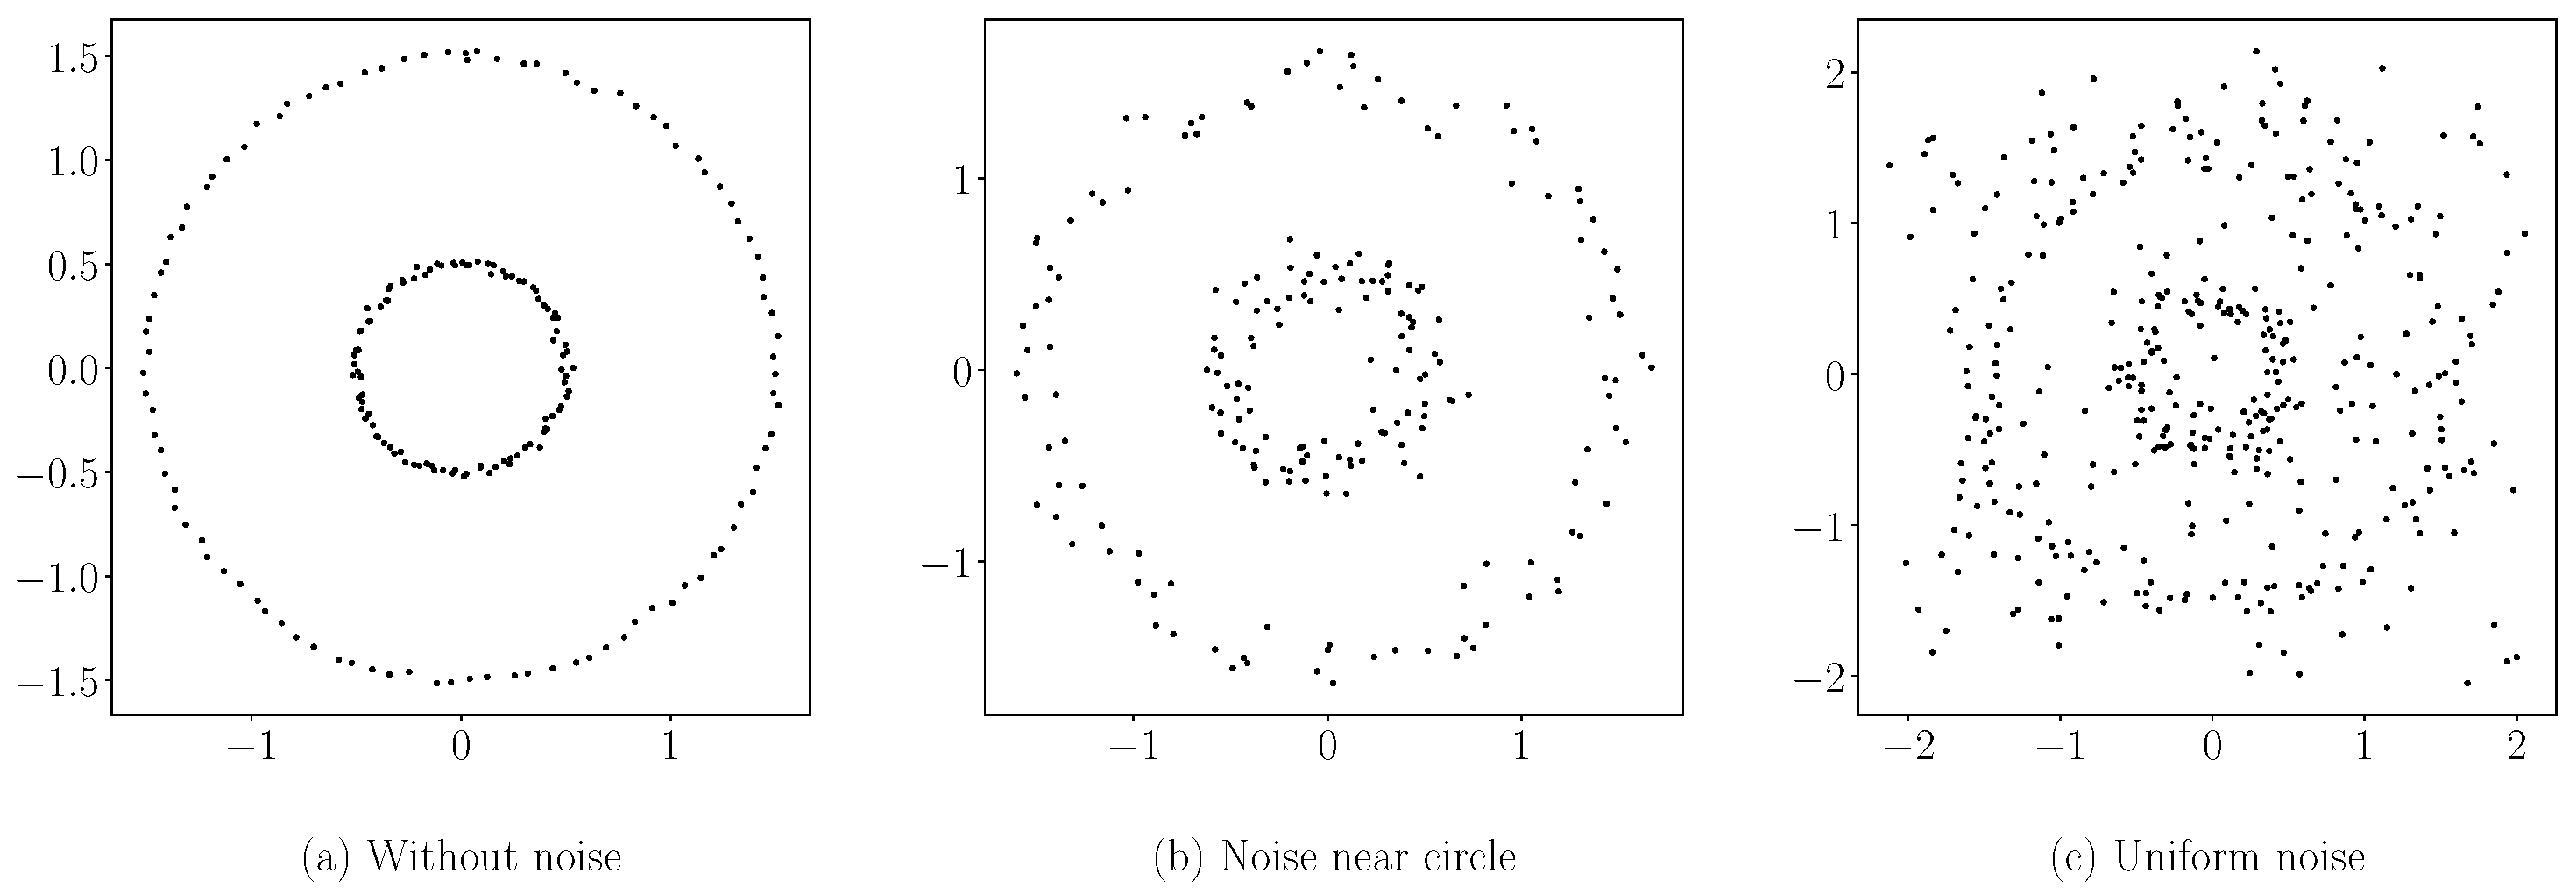
\includegraphics[width=1\textwidth]{results/priorexpert/statment}
\caption{Пример окружностей с разным уровнем шума: (a) окружности без шума; (b) окружности с зашумленным радиусом; (c) окружности с зашумленным радиусом, а также с равномерным шумом по всему изображению}
\label{example:1}
\end{figure}

В данной работе решается задача поиска окружностей на бинаризованном изображении. Предполагается, что радиусы окружностей различаются значимо, а также, что центры почти совпадают. Пример изображений показан на рис. \ref{example:1}. В данной работе в качестве экспертов рассматриваются линейные модели --- каждая модель аппроксимирует одну окружности. В качестве шлюзовой функции рассматривается двухслойная нейронная сеть.

Большое количество работ в области построения смеси экспертов посвящены выбору шлюзовой функции: используется softmax, процесс Дирихле \cite{Edward2002}, нейронная сеть \cite{Shazeer2017} с функцией softmax на последнем слое. Ряд работ посвящены выбору моделей в качестве отдельных экспертов. В работах \cite{Jordan1994, Jordan1991} в качестве модели эксперта рассматривается линейная модель. Работы \cite{Lima2007, Cao2003} рассматриваю модель SVM в качестве модели эксперта.
В работе \cite{Yuksel2012} представлен обзор методов и моделей в задачах смеси экспертов.

Смесь экспертов имеет множество приложений в прикладных задачах. Работы \cite{Yumlu2003, Cheung1995, Weigend2000} посвящены применению смеси экспертов в задачах прогнозирования временных рядов. 
В работе \cite{Ebrahimpour2009} предложен метод распознавания рукописных цифр. 
Метод распознания текстов при помощи смеси экспертов иследуется в работах \cite{Estabrooks2001}, распознание речи \cite{Mossavat2010, Peng1996, Tuerk2001}. 
В работе \cite{Sminchisescu2007} исследуется смесь экспертов для задачи распознавания трехмерных движений человека. 
В \cite{Bowyer2010} описаны работы по исследованию обнаружения радужки глаза на изображении. В работах \cite{Matveev2010, Matveev2014} в частности описаны методы выделения границ радужки и зрачка.

\subsection{Постановка задачи аппроксимации параметров окружности}
Задано бинарное изображение
\[
\label{eq:st:cr:1}
\begin{aligned}
\textbf{M} \in \{0,1\}^{m_1 \times m_2},
\end{aligned}
\]
где $1$ --- это черный пиксель, который принадлежит рассматриваемой фигуре на изображении, а $0$ --- белый пиксель, который является фоном изображения. 
Пример изображения показан на рис. \ref{example:1}.
Изображение $\textbf{M}$ отображается в множество координат \mbox{$\textbf{C}=\left\{x_i, y_i\right\}_{i=1}^{N}$}. Координата $(x_i, y_i)$ является координатой $i$-го черного пикселя на изображении $\textbf{M}$:
\[
\label{eq:st:cr:2}
\begin{aligned}
\textbf{C} \in  \mathbb{R}^{N \times 2},
\end{aligned}
\]
где $N$ --- число черных пикселей.

Обозначим точку $(x_0, y_0)$ центром окружности, а $r$ радиусом окружности.
Координаты $\left(x_i, y_i\right)\in\textbf{C}$ это геометрическое место точек, которое удовлетворяет системе уравнений:
\[
\label{eq:st:cr:3}
\begin{aligned}
\bigr(x_i - x_0\bigr)^{2}+\bigr(y_i-y_0\bigr)^2 = r^2 + \varepsilon_i, \qquad \forall i \in \{1, \cdots, N\},
\end{aligned}
\]
где $\varepsilon_i \in \mathcal{N}\bigr(0, \beta^{-1}\bigr)$ является невязкой $i$-го уравнения, которая является следствием шума на изображении.

Раскрыв скобки получаем:
\[
\label{eq:st:cr:4}
\begin{aligned}
\left(2x_0\right)\cdot x_i + \left(2y_0\right)\cdot y_i+\left(r^2-x_0^2-y_0^2\right)\cdot1 = x_{i}^2 + y_{i}^2 + \varepsilon_i.
\end{aligned}
\]
Выражение \eqref{eq:st:cr:4} переписывается в задачу линейной регрессии следующим образом:
\[
\label{eq:st:cr:5}
\begin{aligned}
\hat{\textbf{w}} = \arg\min_{\textbf{w}\in \mathbf{R}^{n}}||\textbf{X}\textbf{w} - \textbf{y}||,  \quad \textbf{X} = \left[\textbf{C}, \textbf{1}\right], \quad \textbf{y} = \left[x_1^2+y_1^2, x_2^2+y_2^2, \cdots, x_N^2+y_N^2\right]^{\mathsf{T}}.
\end{aligned}
\]
Используя вектор параметров $\hat{\textbf{w}} = \left[w_1, w_2, w_3\right]^{\mathsf{T}}$ получим параметры окружности $x_0, y_0, r$:
\[
\label{eq:st:cr:6}
\begin{aligned}
x_0 = \frac{w_1}{2}, \quad y_0 = \frac{w_2}{2}, \quad r = \sqrt[]{w_3+x_{0}^{2}+y_{0}^{2}}.
\end{aligned}
\]
Решение уравнения \eqref{eq:st:cr:5} находит параметры единственной окружности на изображении. В случае, когда на изображении несколько окружностей, предлагается использовать смесь экспертов, которая состоит из линейных модели --- экспертов. Каждый эксперт описывает одну окружность на изображении.

Обобщим подход аппроксимации одной окружности на изображении на случай, когда на изображении несколько окружностей. Пусть изображение состоит из $K$ окружностей, тогда множество черных пикселей $\textbf{C}$ представляется в виде:
\[
\label{eq:st:1}
\begin{aligned}
\textbf{C} = \sqcup_{k=1}^{K}\textbf{C}_{k}',
\end{aligned}
\]
где $\textbf{C}_{k}'$ множество точек принадлежащих $k$-й окружности. Множеству точек $\textbf{C}_{k}' \subset\textbf{C}$ соответсвует задача линейной регрессии для выборки $\textbf{X}_{k}' \subset \textbf{X}, \textbf{y}_{k}' \subset \textbf{y}$. Модель $\mathbf{g}_k$ аппроксимирующая выборку $\textbf{X}_{k}', \textbf{y}_{k}'$ является локальной моделью для выборки \textbf{X}, \textbf{y}.


\begin{definition}
\label{def:1}
Модель $\mathbf{g}$ называется локальной моделью для выборки $\textbf{U},$ если $\mathbf{g}$ аппроксимирует некоторое не пустое подмножество $\textbf{U}'\subset\textbf{U}$.
\end{definition}

\begin{definition}
\label{def:2}
Мультимодель $\mathbf{f}$ называется смесью экспертов, если:
\[
\label{eq:st:2}
\begin{aligned}
\mathbf{f} = \sum_{k=1}^{K}\pi_{k}\mathbf{g}_k\bigr(\mathbf{w}_k\bigr), \qquad \pi_{k}\bigr(\mathbf{x}, \mathbf{V}\bigr):\mathbb{R}^{n\times \left|\mathbf{V}\right|} \to [0, 1], \qquad \sum_{k=1}^{K}\pi_{k}\bigr(\mathbf{x}, \mathbf{V}\bigr) = 1,
\end{aligned}
\]
где $\mathbf{g}_k$ является $k$-й локальной моделью, $\pi_k$ --- шлюзовая функция, вектор $\mathbf{w}_k$ является параметрами $k$-й локальной моделью, а $\mathbf{V}$ --- параметры шлюзовой функции.
\end{definition}

В данной работе в качестве локальных моделей рассматриваются линейные модели. В качестве шлюзовой функции рассматривается двухслойный перцептрон:
\[
\label{eq:st:3}
\begin{aligned}
\mathbf{g}_k\bigr(\textbf{x}\bigr) = \textbf{w}_k^{\mathsf{T}}\textbf{x}, \quad
\bm{\pi}\bigr(\mathbf{x}, \mathbf{V}\bigr) = \text{softmax}\bigr(\mathbf{V}_{1}^{\mathsf{T}}\bm{\sigma}\bigr(\mathbf{V}_2^{\mathsf{T}}\mathbf{x}\bigr)\bigr),
\end{aligned}
\]
где $\mathbf{V} = \bigr\{\mathbf{V}_1, \mathbf{V}_2\bigr\}$ --- множество параметров шлюзовой функции.

В статье предлагается использовать вероятностный подход для описания смеси экспертов. Вводиться предположение, что $\textbf{y}$ является случайным вектором, который задается плотностью распределения $p\bigr(\textbf{y}|\textbf{X}\bigr)$. Предполагается, что плотность распределения $p\bigr(\textbf{y}|\textbf{X}, \textbf{f}\bigr)$ аппроксимирует истинную плотность распределения $p\bigr(\textbf{y}|\textbf{X}\bigr)$:
\[
\label{eq:st:new:1}
\begin{aligned}
p\bigr(\textbf{y}|\textbf{X}, \textbf{f}\bigr) = \prod_{i=1}^{N}\left(\sum_{k=1}^{K}\pi_kp_{k}\bigr(y_{i}|\textbf{g}_{k}\bigr(\mathbf{x}_{i}\bigr)\bigr)\right),
\end{aligned}
\]
где $\textbf{f}$ --- это смесь экспертов, а $\textbf{g}_k, \bm{\pi}$ определяются выражением \eqref{eq:st:3}.

Пусть $\textbf{w}_k$ является случайным вектором, который задается плотностью распределения $p^{k}\bigr(\mathbf{w}_k\bigr)$. Получим совместное распределения параметров локальных моделей и вектора ответов:
\[
\label{eq:st:4}
\begin{aligned}
p\bigr(\mathbf{y}, \mathbf{W}|\mathbf{X}, \mathbf{V}\bigr) = \prod_{k=1}^{K}p^{k}\bigr(\mathbf{w}_k\bigr)\prod_{i=1}^{N}\left(\sum_{k=1}^{K}\pi_{k}p_{k}\bigr(y_i|\mathbf{w}_k, \mathbf{x}_i\bigr)\right),
\end{aligned}
\]
где $\mathbf{W} = \bigr\{\mathbf{w}_1, \mathbf{w}_2, \cdots, \mathbf{w}_K\bigr\}.$
Оптимальные параметры находятся при помощи максимизации правдоподобия:
\[
\label{eq:st:5}
\begin{aligned}
\hat{\mathbf{V}}, \hat{ \mathbf{W}} = \arg\max_{\mathbf{V}, \mathbf{W}} p\bigr(\mathbf{y},  \mathbf{W}|\mathbf{X}, \mathbf{V}\bigr).
\end{aligned}
\]

\subsection{Вероятностная постановка задачи смеси экспертов}
Для построения смеси экспертов (\ref{eq:st:2},  \ref{eq:st:4}), введем следующие вероятностные предположения о данных \eqref{eq:st:cr:5}:

\begin{enumerate}
	\item[1)] правдоподобие $p_{k}\bigr(y_{i}|\mathbf{w}_{k}, \mathbf{x}_{i}\bigr) = \mathcal{N}\bigr(y_{i}|\mathbf{w}_{k}^{\mathsf{T}}\mathbf{x}_{i}, \beta^{-1}\bigr),$ где параметр $\beta$ является уровнем шума,
	\item[2)] априорное распределение параметров $p^{k}\bigr(\mathbf{w}_{k}\bigr) = \mathcal{N}\bigr(\mathbf{w}_{k}|\mathbf{w}^{0}_{k}, \mathbf{A}_{k}\bigr),$ где $\mathbf{w}^{0}_{k}$ --- вектор размерности $n\times1$, а  $\mathbf{A}_{k}$ --- ковариационная матрица размерности $n\times n$,
	\item[3)] регуляризация априорного распределения $p\bigr(\bm{\varepsilon}_{k,k'}|\bm{\Xi}\bigr) = \mathcal{N}\bigr(\bm{\varepsilon}_{k,k'}|\mathbf{0},  \bm{\Xi}\bigr),$ где $\bm{\Xi}$ --- ковариационная матрица, а $\bm{\varepsilon}_{k,k'} = \mathbf{w}_{k}^{0}-\mathbf{w}_{k'}^{0}.$
\end{enumerate}
Предположение 2) задает априорное предположения на вектора параметров локальных модели $\textbf{w}_k$. Априорное распределение  задает ограничения на локальную модель. Например, если $\textbf{w}_k^{0} = [0,0,1]$, то $k$-я локальная модель аппроксимирует окружность с параметрами $x_0=0, y_0=0, r=1$ с большей вероятностью.

Предположения 3) задает регулярицию априорных распределений. Данная регулярицая учитывает связь между априорными ограничениями разных локальных моделей. Например, если $\text{diag}\bigr(\bm{\Xi}\bigr)=[0.001, 0.001, 1]$, то  центры разных окружностей совпадают.

Используя предположения $1), 2), 3)$ и выражение \eqref{eq:st:4} получаем полное правдоподобие:
\[
\label{eq:em:1}
\begin{aligned}
p\bigr(\mathbf{y}, \mathbf{W}|\mathbf{X}, \mathbf{V}, \textbf{A}, \textbf{W}^{0}, \bm{\Xi}, \beta\bigr) = &\prod_{i=1}^{N}\left(\sum_{k=1}^{K}\pi_{k}\mathcal{N}\bigr(y_{i}|\mathbf{w}_{k}^{\mathsf{T}}\mathbf{x}_{i}, \beta^{-1}\bigr)\right)\cdot\\
&\cdot\prod_{k=1}^{K}\mathcal{N}\bigr(\mathbf{w}_{k}|\mathbf{w}^{0}_{k}, \mathbf{A}_{k}\bigr)\cdot\prod_{k,k'=1}^{K}\mathcal{N}\bigr(\bm{\varepsilon}_{k,k'}|\mathbf{0},  \bm{\Xi}\bigr),
\end{aligned}
\]

 где $\mathbf{A} = \left\{\mathbf{A}_1, \cdots, \mathbf{A}_K\right\}.$
 
Введем бинарную матрицу $\mathbf{Z}$. Элемент матрицы $z_{ik}$ равно $1$ тогда и только тогда, когда $i$-й объект аппроксимируется $k$-й локальной моделью.
Подставляя бинарную матрицу $\mathbf{Z}$ в выражении \eqref{eq:em:1}, а также взяв логарифм получаем:
\[
\label{eq:em:2}
\begin{aligned}
\log p\bigr(\mathbf{y}, \mathbf{Z}, \mathbf{W}&|\mathbf{X}, \mathbf{V}, \textbf{A}, \textbf{W}^{0},  \bm{\Xi}, \beta\bigr) =\\
&= \sum_{i=1}^{N}\sum_{k=1}^{K}z_{ik}\left[\log\pi_k\bigr(\textbf{x}_i, \textbf{V}\bigr) - \frac{\beta}{2}\left(y_{i} - \textbf{w}_{k}^{\mathsf{T}}\textbf{x}_{i}\right)^{2} + \frac{1}{2}\log\frac{\beta}{2\pi}\right] +\\
&+ \sum_{k=1}^{K}\left[-\frac{1}{2}\left(\textbf{w}_{k} - \textbf{w}_{k}^{0}\right)^{\mathsf{T}}\textbf{A}_{k}^{-1}\left(\textbf{w}_{k} - \textbf{w}_{k}^{0}\right) + \frac{1}{2}\log\det\textbf{A}^{-1}_{k} - \frac{n}{2}\log2\pi\right]+\\
&+ \sum_{k=1}^{K}\sum_{k'=1}^{K}\left[-\frac{1}{2}\left(\textbf{w}_{k}^{0}-\textbf{w}_{k'}^{0}\right)^{\mathsf{T}}\bm{\Xi}^{-1}\left(\textbf{w}_{k}^{0}-\textbf{w}_{k'}^{0}\right) +\frac{1}{2}\log\det \bm{\Xi} -\frac{n}{2}\log{2\pi}\right].
\end{aligned}
\]
Получаем новую задачу оптимизации обоснованности. Функция обоснованности получается при интегрировании выражения \eqref{eq:em:2} по параметрам $\textbf{W}, \textbf{Z}$:
\[
\label{eq:em:3}
\begin{aligned}
\mathbf{V}, \mathbf{W}^0, \textbf{A},  \beta = \arg\max_{\mathbf{V}, \mathbf{W}^0, \textbf{A}, \beta} \int_{\textbf{W}, \textbf{Z}}\log p\bigr(\mathbf{y}, \textbf{Z}, \textbf{W}|\mathbf{X}, \mathbf{V}, \textbf{A}, \textbf{W}^{0}, \bm{\Xi}, \beta\bigr)d\textbf{W}d\textbf{Z}.
\end{aligned}
\]
Рассмотрим вариационную плотность $q\bigr(\textbf{W}, \textbf{Z}\bigr)$ для параметров $\textbf{W}, \textbf{Z}$. Тогда функция обоснованности принимает следующий вид:
\[
\label{eq:em:new:1}
\begin{aligned}
\log p\bigr(\mathbf{y}|\mathbf{X}, \mathbf{V}, \textbf{A}, \textbf{W}^{0}, \bm{\Xi}, \beta\bigr) &= \int_{\textbf{W}, \textbf{Z}} q\bigr(\textbf{W}, \textbf{Z}\bigr) \log p\bigr(\mathbf{y}|\mathbf{X}, \mathbf{V}, \textbf{A}, \textbf{W}^{0}, \bm{\Xi}, \beta\bigr)d\textbf{W}d\textbf{Z} =\\
&= \int_{\textbf{W}, \textbf{Z}} q\bigr(\textbf{W}, \textbf{Z}\bigr)\log \frac{p\bigr(\mathbf{y}, \textbf{W}, \textbf{Z}|\mathbf{X}, \mathbf{V}, \textbf{A}, \textbf{W}^{0}, \bm{\Xi}, \beta\bigr)}{p\bigr(\textbf{W}, \textbf{Z}|\mathbf{y}, \mathbf{X}, \mathbf{V}, \textbf{A}, \textbf{W}^{0}, \bm{\Xi}, \beta\bigr)}d\textbf{W}d\textbf{Z}=\\
&= \int_{\textbf{W}, \textbf{Z}} q\bigr(\textbf{W}, \textbf{Z}\bigr)\log \frac{p\bigr(\mathbf{y}, \textbf{W}, \textbf{Z}|\mathbf{X}, \mathbf{V}, \textbf{A}, \textbf{W}^{0}, \bm{\Xi}, \beta\bigr)q\bigr(\textbf{W}, \textbf{Z}\bigr)}{p\bigr(\textbf{W}, \textbf{Z}|\mathbf{y}, \mathbf{X}, \mathbf{V}, \textbf{A}, \textbf{W}^{0}, \bm{\Xi}, \beta\bigr)q\bigr(\textbf{W}, \textbf{Z}\bigr)}d\textbf{W}d\textbf{Z}=\\
&= \int_{\textbf{W}, \textbf{Z}} q\bigr(\textbf{W}, \textbf{Z}\bigr)\frac{p\bigr(\mathbf{y}, \textbf{W}, \textbf{Z}|\mathbf{X}, \mathbf{V}, \textbf{A}, \textbf{W}^{0}, \bm{\Xi}, \beta\bigr)}{q\bigr(\textbf{W}, \textbf{Z}\bigr)}d\textbf{W}d\textbf{Z}+\\
&+\int_{\textbf{W}, \textbf{Z}} q\bigr(\textbf{W}, \textbf{Z}\bigr)\frac{q\bigr(\textbf{W}, \textbf{Z}\bigr)}{p\bigr(\textbf{W}, \textbf{Z}|\mathbf{y}, \mathbf{X}, \mathbf{V}, \textbf{A}, \textbf{W}^{0}, \bm{\Xi}, \beta\bigr)}d\textbf{W}d\textbf{Z}=\\
&=\mathcal{L}\bigr(q, \textbf{V}, \textbf{W}^{0}, \textbf{A}, \beta\bigr)+\mathsf{D}_{KL}\left(q\bigr(\textbf{W}, \textbf{Z}\bigr)||p\bigr(\textbf{W}, \textbf{Z}|\mathbf{y}, \mathbf{X}, \mathbf{V}, \textbf{A}, \textbf{W}^{0}, \bm{\Xi}, \beta\bigr)\right)
\end{aligned}
\]
Используя \eqref{eq:em:new:1} получаем нижнюю оценку обоснованости:
\[
\label{eq:em:new:2}
\begin{aligned}
\log p\bigr(\mathbf{y}|\mathbf{X}, \mathbf{V}, \textbf{A}, \textbf{W}^{0}, \bm{\Xi}, \beta\bigr)\geq \mathcal{L}\bigr(q, \textbf{V}, \textbf{W}^{0}, \textbf{A}, \beta\bigr),
\end{aligned}
\]
где $\mathcal{L}\bigr(q, \textbf{V}, \textbf{W}^{0}, \textbf{A}, \beta\bigr)$ называется нижней оценкой обоснованости.

Используем EM--алгоритм \cite{Dempster1977, bishop2006} для решения оптимизационной задачи \eqref{eq:em:3}. Заметим, что EM--алгоритм вместо оптимизации $\log p\bigr(\mathbf{y}|\mathbf{X}, \mathbf{V}, \textbf{A}, \textbf{W}^{0}, \bm{\Xi}, \beta\bigr)$ оптимизирует нижнюю оценку $\mathcal{L}\left(q, \textbf{V}, \textbf{W}^{0}, \textbf{A}, \beta\right)$.


\paragraph{E-шаг.} E-шаг решает следующую оптимизационую задачу:
\[
\label{eq:em:new:3}
\begin{aligned}
\mathcal{L}\bigr(q, \textbf{V}, \textbf{W}^{0}, \textbf{A}, \beta\bigr) \to \max_{q\bigr(\textbf{W}, \textbf{Z}\bigr)},
\end{aligned}
\]
где параметры $\textbf{V}, \textbf{W}^{0}, \textbf{A}, \beta$ являются зафиксированными.

Пусть совместное распределение $q\bigr(\mathbf{Z}, \mathbf{W}\bigr)$ удовлетворяет условию независимости $q\bigr(\mathbf{Z}, \mathbf{W}\bigr) = q\bigr(\mathbf{Z}\bigr)q\bigr(\mathbf{W}\bigr)$ \cite{bishop2006}. 
Далее символом $\propto$ обозначим то, что обе стороны выражения равны с точностью до аддитивной константы.
Сначала найдем распределение $q\bigr(\textbf{Z}\bigr)$:
\[
\label{eq:em:4}
\begin{aligned}
\log q\bigr(\textbf{Z}\bigr) &= \mathsf{E}_{q/\textbf{Z}} \log p\bigr(\mathbf{y}, \mathbf{Z}, \mathbf{W}|\mathbf{X}, \mathbf{V}, \textbf{A}, \textbf{W}^{0}, \bm{\Xi}, \beta\bigr)  \propto\\
&\propto \sum_{i+1}^{N}\sum_{k=1}^{K}z_{ik}\left[\log\pi_{k}\bigr(\textbf{x}_{i}, \textbf{V}\bigr) - \frac{\beta}{2}\left(y_{i}^{2} -\textbf{x}_{i}^{\mathsf{T}}\mathsf{E}\textbf{w}_{k} + \textbf{x}_{i}^{\mathsf{T}}\mathsf{E}\textbf{w}_{k}\textbf{w}_{k}^{\mathsf{T}}\textbf{x}_{i}\right) + \frac{1}{2}\log\frac{\beta}{2\pi}\right]\\
p\bigr(z_{ik} = 1\bigr) &= \frac{\exp\bigr(\log\pi_{k}\bigr(\textbf{x}_{i}, \textbf{V}\bigr) - \frac{\beta}{2}\left(\textbf{x}_{i}^{\mathsf{T}}\mathsf{E}\textbf{w}_{k}\textbf{w}_{k}^{\mathsf{T}}\textbf{x}_{i} - \textbf{x}_{i}^{\mathsf{T}}\mathsf{E}\textbf{w}_{k}\right)\bigr)}{\sum_{k'=1}^{K}\exp\bigr(\log\pi_{k'}\bigr(\textbf{x}_{i}, \textbf{V}\bigr) - \frac{\beta}{2}\left(\textbf{x}_{i}^{\mathsf{T}}\mathsf{E}\textbf{w}_{k'}\textbf{w}_{k'}^{\mathsf{T}}\textbf{x}_{i} - \textbf{x}_{i}^{\mathsf{T}}\mathsf{E}\textbf{w}_{k'}\right)\bigr)}.
\end{aligned}
\]
Используя выражения \eqref{eq:em:4} получаем, что распределение $q\bigr(z_{ik}\bigr)$ является бернулевским распределением с параметром $z_{ik},$ которое задается выражением \eqref{eq:em:4}.
Далее найдем распределение $q\bigr(\textbf{W}\bigr)$:
\[
\label{eq:em:5}
\begin{aligned}
\log q\bigr(\textbf{W}\bigr) &= \mathsf{E}_{q/\textbf{W}}\log p\bigr(\mathbf{y}, \mathbf{Z}, \mathbf{W}|\mathbf{X}, \mathbf{V}, \textbf{A}, \textbf{W}^{0}, \bm{\Xi}, \beta\bigr) \propto\\
&\propto \sum_{i=1}^{N}\sum_{k=1}^{K}\mathsf{E}z_{ik}\left[\log\pi_{k}\bigr(\textbf{x}_{i, \textbf{V}}\bigr) - \frac{\beta}{2}\left(y_{i} - \textbf{w}_{k}^{\mathsf{T}}\textbf{x}_{i}\right)^{2} + \frac{1}{2}\log\frac{\beta}{2\pi}\right] + \\
&+ \sum_{k=1}^{K}\left[-\frac{1}{2}\left(\textbf{w}_{k} - \textbf{w}_{k}^{0}\right)^{\mathsf{T}}\textbf{A}_{k}^{-1}\left(\textbf{w}_{k} - \textbf{w}_{k}^{0}\right) + \frac{1}{2}\log\det\textbf{A}^{-1}_{k} - \frac{n}{2}\log2\pi\right] \\
&\propto \sum_{k=1}^{K}\left[\textbf{w}_{k}^{\mathsf{T}}\left(\textbf{A}_{k}^{-1}\textbf{w}_{k}^{0}+\beta\sum_{i=1}^{N}\textbf{x}_{i}y_{i}\mathsf{E}z_{ik}\right)-\frac{1}{2}\textbf{w}_{k}^{\mathsf{T}}\left(\textbf{A}_{k}^{-1}+\beta\sum_{i=1}^{N}\textbf{x}_{i}\textbf{x}_{i}^{\mathsf{T}}\right)\textbf{w}_{k}\right].
\end{aligned}
\]
Используя выражение \eqref{eq:em:5} получаем, что  распределение $q\bigr(\mathbf{w}_{k}\bigr)$ является нормальным распределением со средним $\mathbf{m}_{k}$ и ковариационной матрицей $\mathbf{B}_k$:
\[
\label{eq:em:6}
\begin{aligned}
\mathbf{m}_{k} = \mathbf{B}_{k}\left(\mathbf{A}_{k}^{-1}\mathbf{w}_{k}^{0}+\beta\sum_{i=1}^{N}\mathbf{x}_{i}y_{i}\mathsf{E}z_{ik}\right), \qquad \mathbf{B}_{k} = \left(\mathbf{A}_{k}^{-1}+\beta\sum_{i=1}^{N}\mathbf{x}_{i}\mathbf{x}_{i}^{\mathsf{T}}\mathsf{E}z_{ik}\right)^{-1}.
\end{aligned}
\]

\paragraph{M-шаг.} M-шаг решает следующую оптимизационную задачу:
\[
\label{eq:em:new:3}
\begin{aligned}
\mathcal{L}\bigr(q, \textbf{V}, \textbf{W}^{0}, \textbf{A}, \beta\bigr) \to \max_{\textbf{V}, \textbf{W}^{0}, \textbf{A}, \beta},
\end{aligned}
\]
где $q\bigr(\textbf{W}, \textbf{Z}\bigr)$ является известной плотностью распределения.
Распределение $q\bigr(\mathbf{Z}, \mathbf{W}\bigr)$ является фиксированным, в то время как вариацонная нижняя оценка $\mathcal{L}\bigr(\textbf{V}, \textbf{W}^{0}, \textbf{A}, \beta\bigr)$ максимизируется по параметрам $\mathbf{V}, \mathbf{W}^0, \textbf{A},  \beta$:
\[
\label{eq:em:7}
\begin{aligned}
\mathcal{L}\bigr(\textbf{V}, \textbf{W}^{0}, \textbf{A}, \beta\bigr) &= \mathsf{E}_{q}\log p\bigr(\mathbf{y}, \mathbf{Z}, \mathbf{W}|\mathbf{X}, \mathbf{V}, \textbf{A}, \textbf{W}^{0}, \bm{\Xi}, \beta\bigr) =  \\
&= \sum_{i=1}^{N}\sum_{k=1}^{K}\mathsf{E}z_{ik}\left[\log\pi_k\bigr(\textbf{x}_i, \textbf{V}\bigr) - \frac{\beta}{2}\mathsf{E}\left(y_{i} - \textbf{w}_{k}^{\mathsf{T}}\textbf{x}_{i}\right)^{2} + \frac{1}{2}\log\frac{\beta}{2\pi}\right] +\\
&+ \sum_{k=1}^{K}\left[-\frac{1}{2}\mathsf{E}\left(\textbf{w}_{k} - \textbf{w}_{k}^{0}\right)^{\mathsf{T}}\textbf{A}_{k}^{-1}\left(\textbf{w}_{k} - \textbf{w}_{k}^{0}\right) + \frac{1}{2}\log\det\textbf{A}^{-1}_{k} - \frac{n}{2}\log2\pi\right] +\\
&+ \sum_{k=1}^{K}\sum_{k'=1}^{K}\left[-\frac{1}{2}\left(\textbf{w}_{k}^{0}-\textbf{w}_{k'}^{0}\right)^{\mathsf{T}}\bm{\Xi}^{-1}\left(\textbf{w}_{k}^{0}-\textbf{w}_{k'}^{0}\right) +\frac{1}{2}\log\det\bm{\Xi} -\frac{n}{2}\log{2\pi}\right].
\end{aligned}
\]
Во-первых, для нахождения оптимального параметра $\textbf{V}$ используется градиентный метод оптимизации, который сходится к некоторому локальному экстремуму.
Во вторых, используя выражения \eqref{eq:em:7} получаем оптимальное значения параметра $\textbf{A}_{k}$
\[
\label{eq:em:9}
\begin{aligned}
\frac{\partial \mathcal{L}\bigr(\textbf{V}, \textbf{W}^{0}, \textbf{A}, \beta\bigr)}{\partial \textbf{A}^{-1}_k} &=  \frac{1}{2}\textbf{A}_{k} - \frac{1}{2}\mathsf{E}\left(\textbf{w}_{k} - \textbf{w}_{k}^{0}\right)\left(\textbf{w}_{k} - \textbf{w}_{k}^{0}\right)^{\mathsf{T}} = 0,\\
\textbf{A}_{k} &= \mathsf{E}\textbf{w}_{k}\textbf{w}_{k}^{\mathsf{T}} - \textbf{w}_{k}^{0}\mathsf{E}\textbf{w}_{k}^{\mathsf{T}} - \mathsf{E}\textbf{w}_{k}\textbf{w}_{k}^{0\mathsf{T}} + \textbf{w}_{k}^{0}\textbf{w}_{k}^{0\mathsf{T}}.
\end{aligned}
\]
Аналогично получаем оптимальные значения для параметра $\beta$ и для параметров $\textbf{w}_{k}^{0}$
\[
\label{eq:em:10}
\begin{aligned}
\frac{\partial \mathcal{L}\bigr(\textbf{V}, \textbf{W}^{0}, \textbf{A}, \beta\bigr)}{\partial \beta} &= \sum_{k=1}^{K}\sum_{i=1}^{N}\left(\frac{1}{\beta}\mathsf{E}z_{ik}-\frac{1}{2}\mathsf{E}z_{ik}\left[y_{i}^{2}-2y_{i}\textbf{x}_{i}^{\mathsf{T}}\mathsf{E}\textbf{w}_{k}+\textbf{x}_{i}^{\mathsf{T}}\textbf{w}_{k}\textbf{w}_{k}^{\mathsf{T}}\textbf{x}_{i}\right]\right) = 0,\\
\frac{1}{\beta}&=\frac{1}{N}\sum_{i=1}^{N}\sum_{k=1}^{K}\left[y_{i}^{2}-2y_{i}\textbf{x}_{i}^{\mathsf{T}}\mathsf{E}\textbf{w}_{k} + \textbf{x}_{i}^{\mathsf{T}}\mathsf{E}\textbf{w}_{k}\textbf{w}_{k}^{\mathsf{T}}\textbf{x}_{i}\right]\mathsf{E}z_{ik}.
\end{aligned}
\]
\[
\label{eq:em:11}
\begin{aligned}
\frac{\partial \mathcal{L}\bigr(\textbf{V}, \textbf{W}^{0}, \textbf{A}, \beta\bigr)}{\partial \mathbf{w}_k^0} &= \mathbf{A}_k^{-1}\left(\mathsf{E}\mathbf{w}_k - \mathbf{w}_{k}^{0}\right) + \bm{\Xi}\sum_{k'=1}^{K}\bigr[\mathbf{w}_{k'}^{0} -\mathbf{w}_{k}^{0}\bigr] = 0,\\
\textbf{w}_{k}^{0} &=\left[\textbf{A}_{k}^{-1}+\left(K-1\right)\bm{\Xi}\right]^{-1}\left(\textbf{A}^{-1}_{k}\mathsf{E}\textbf{w}_{k}+\bm{\Xi}\sum_{k'=1, k'\not=k}^{K}\textbf{w}_{k'}^{0}\right).
\end{aligned}
\]
Выражения (\ref{eq:em:4}--\ref{eq:em:11}) задают итеративную процедуру, которая сходится к некоторому локальному максимуму оптимизационной задачи \eqref{eq:em:3}.

\subsection{Вычислительный эксперимент по анализу качества аппроксимации радужки глаза смесью экспертов}
Для анализа качества различных мультимоделей для аппроксимации окружности проводится вычислительный эксперимент.
В эксперимент рассматриваются следующие мультимодели: мультимодель $\textbf{f}_1$ без использования априорных распределений, мультимодель $\textbf{f}_2,$ которая использует априорные распределения \eqref{eq:ce:1} для параметров и мультимодель $\textbf{f}_3,$ которая использует регуляризацию априорных распределений.
Точность аппроксимации мультимодели $\textbf{f}_i$ задается следующим образом:
\[
\label{eq:ce:ex:0:1}
\begin{aligned}
\mathcal{S}_{\textbf{f}_i} = \sum_{k=1}^{K}\bigr(x^{k}_{0}-x^{k}_{\text{pr}}\bigr)^2+\bigr(y^{k}_{0}-y^{k}_{\text{pr}}\bigr)^2+\bigr(r^{k}-r^{k}_{\text{pr}}\bigr)^2,
\end{aligned}
\]
где $x^{k}_0, y^{k}_0, r^{k}$ является истинным центром и радиусом для $k$-й окружности, $x^{k}_{\text{pr}}, y^{k}_{\text{pr}}, r^{k}_{\text{pr}}$ является предсказанным центром и радиусом для $k$-й окружности.

Для сравнение модель с разными вероятностными предположениями используется правдоподобие  \eqref{eq:st:new:1}.
В вычислительном эксперименте используется следующее априорное распределение:
\[
\label{eq:ce:1}
\begin{aligned}
p^{1}\bigr(\textbf{w}_1\bigr)\sim\mathcal{N}\bigr(\textbf{w}^{0}_{1}, \textbf{I}\bigr), \quad p^{2}\bigr(\textbf{w}_2\bigr)\sim\mathcal{N}\bigr(\textbf{w}^{0}_{2}, \textbf{I}\bigr),
\end{aligned}
\]
где $\textbf{w}^{0}_1 = [0, 0, 0.1],\ \textbf{w}^{0}_2 = [0, 0, 2]$.

\paragraph{Синтетические данные с разным типом шума в изображении.}
\begin{figure}[h!t]\center
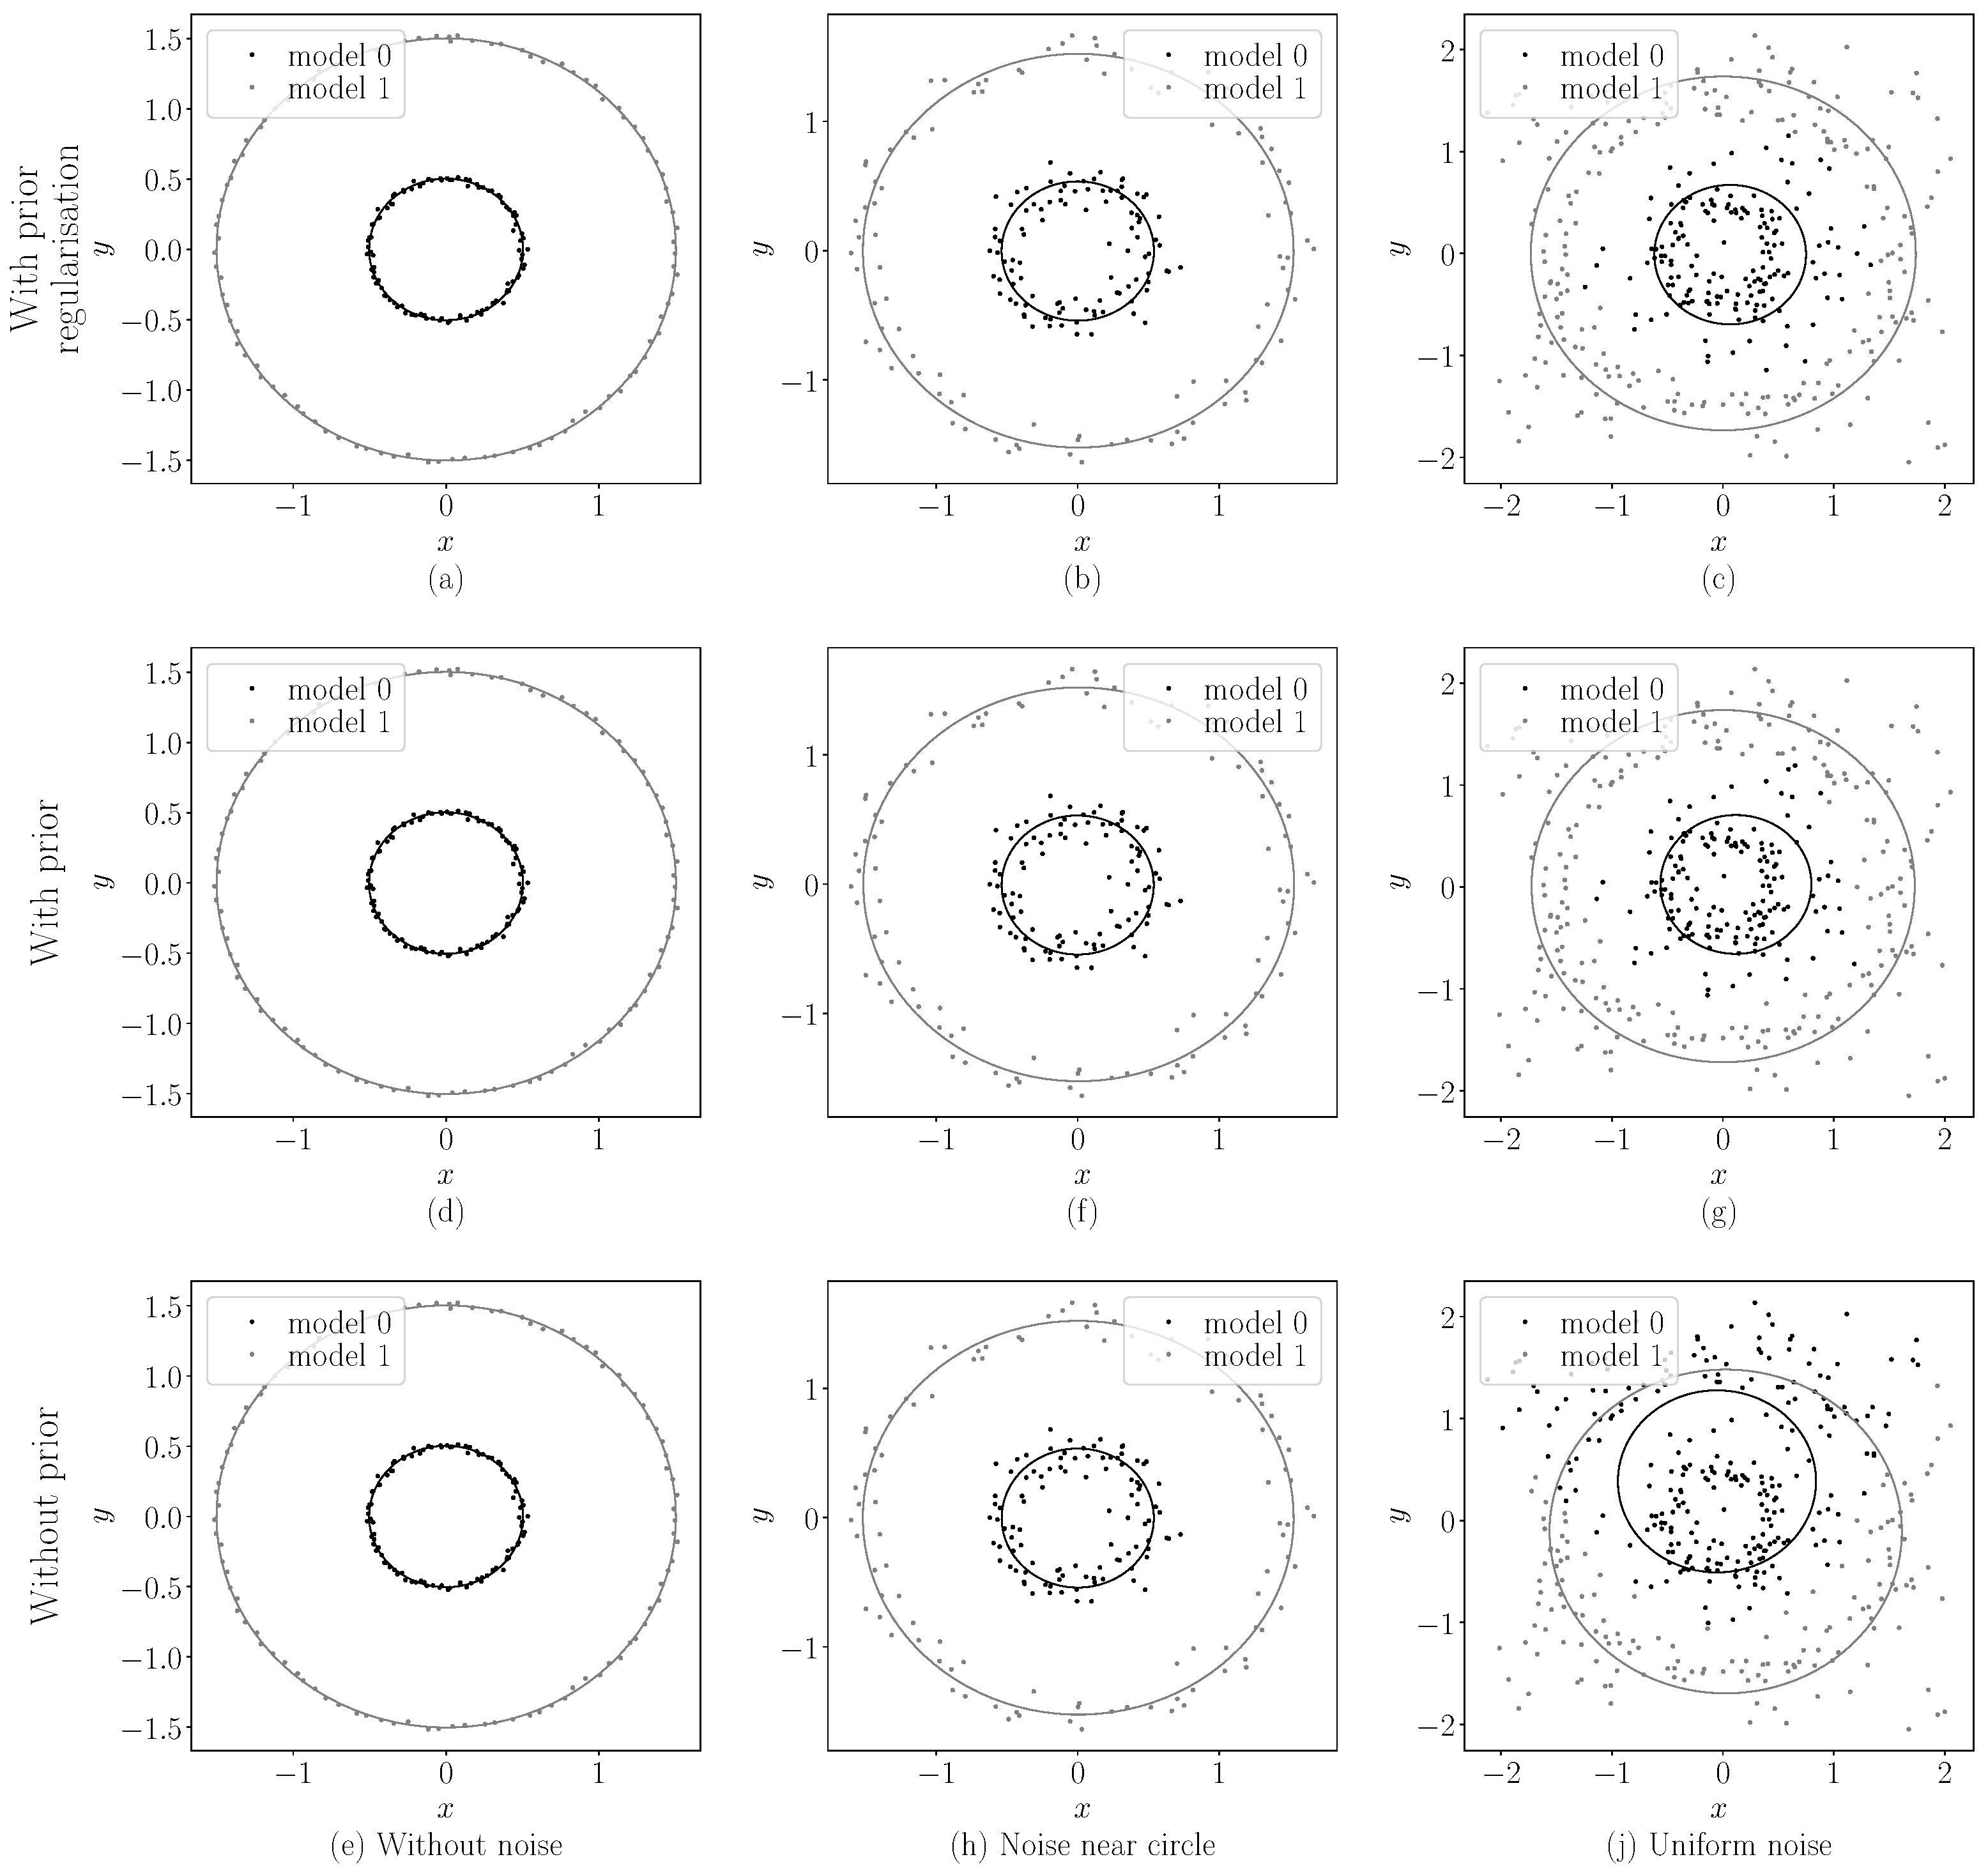
\includegraphics[width=1\textwidth]{results/priorexpert/experiment_synthetic}
\caption{Мультимодель в зависимости от разных априорных предположений и в зависимости от разного уровня шума: (a)--(с) модель с регуляризаций априорных распределений; (d)--(g) модель с заданными априорными распределениями на параметрах локальных моделей; (e)--(j) модель без заданных априорных предположений}
\label{experiment:1}
\end{figure}
В вычислительном эксперименте сравнивается качество следующих мультимоделей $\textbf{f}_1, \textbf{f}_2, \textbf{f}_3$ на синтетических данных.
Синтетические данные являются двумя концентрическими окружностями с разным уровнем шума.
Выборка Synthetic 1 является изображением без шума, выборка Synthetic 2 изображение с зачумлённым радиусом окружности, а выборка Synthetic 3 --- изображение с равномерным шумом.
На рис. \ref{experiment:1} показаны результаты для мельтимоделей $\textbf{f}_1, \textbf{f}_2, \textbf{f}_3$.
Все модели оптимизировались при помощи 50 итераций EM-алгоритма.
Мультимодели $\textbf{f}_2, \textbf{f}_3$ аппроксимируют окружности лучше чем мультимодель $\textbf{f}_1$. В табл. \ref{tb:ce:1} показано качество аппрроксимации \eqref{eq:ce:ex:0:1} для всех мультимоделей.

\begin{table}[h!t]
\begin{center}
\caption{Качество аппроксимации \eqref{eq:ce:ex:0:1} для всех мультимоделей}
\label{tb:ce:1}
\begin{tabular}{|c|c|c|c|}
\hline
	Выборка & $\mathcal{S}_{\textbf{f}_1}$ & $\mathcal{S}_{\textbf{f}_2} $& $\mathcal{S}_{\textbf{f}_3} $\\
	\hline
	\multicolumn{1}{|l|}{Synthetic 1}
	& $10^{-5}$& $10^{-5}$& $10^{-5}$\\
	\hline
	\multicolumn{1}{|l|}{Synthetic 2}
	& $0.6$& $10^{-3}$& $10^{-3}$\\
	\hline
	\multicolumn{1}{|l|}{Synthetic 3}
	& $0.6$& $10^{-3}$& $10^{-3}$\\
\hline
\end{tabular}
\end{center}
\end{table}

\paragraph{Анализ сходимости на синтетической выборке.}
\begin{figure}[h!t]\center
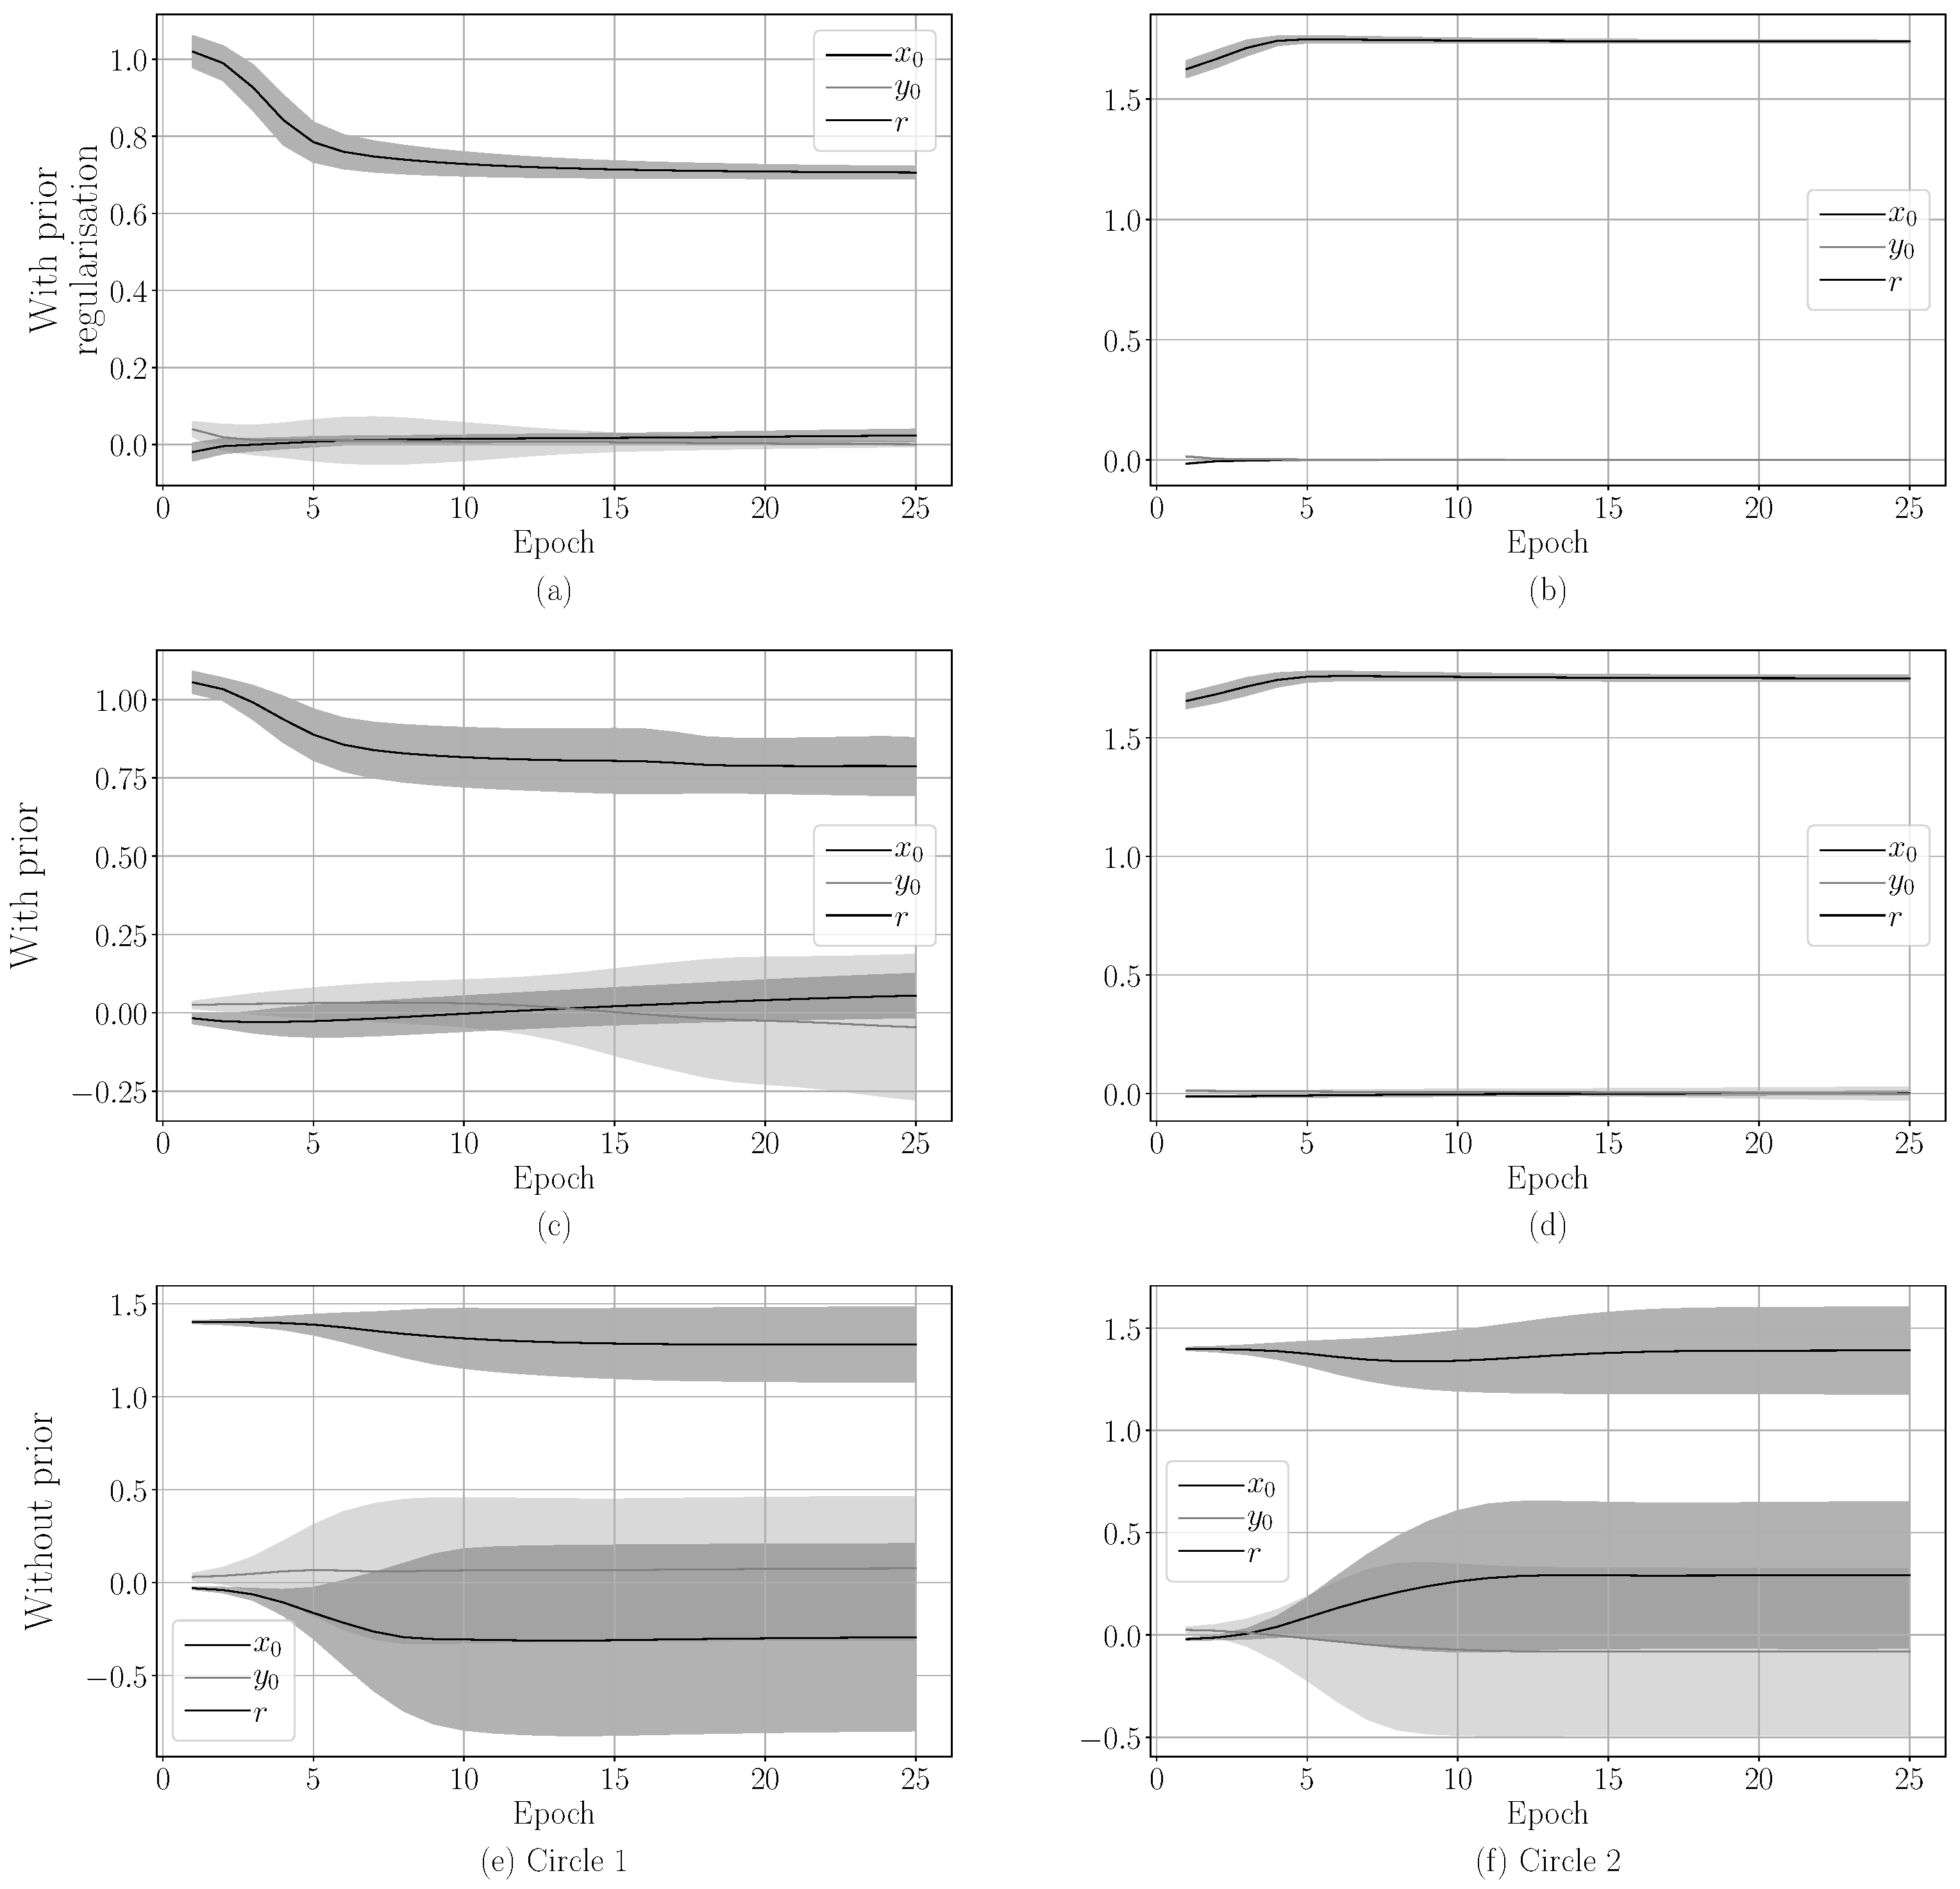
\includegraphics[width=1\textwidth]{results/priorexpert/experiment_synthetic_param_progress}
\caption{График зависимости центра и радиуса окружностей от номера итерации: (a)--(b) модель с регуляризацией априорных распределений; (c)--(d) модель с заданными априорными распределениями на параметры моделей; (e)--(f) модель без задания априорных распределений}
\label{experiment:st:2:1}
\end{figure}

\begin{figure}[h!t]\center
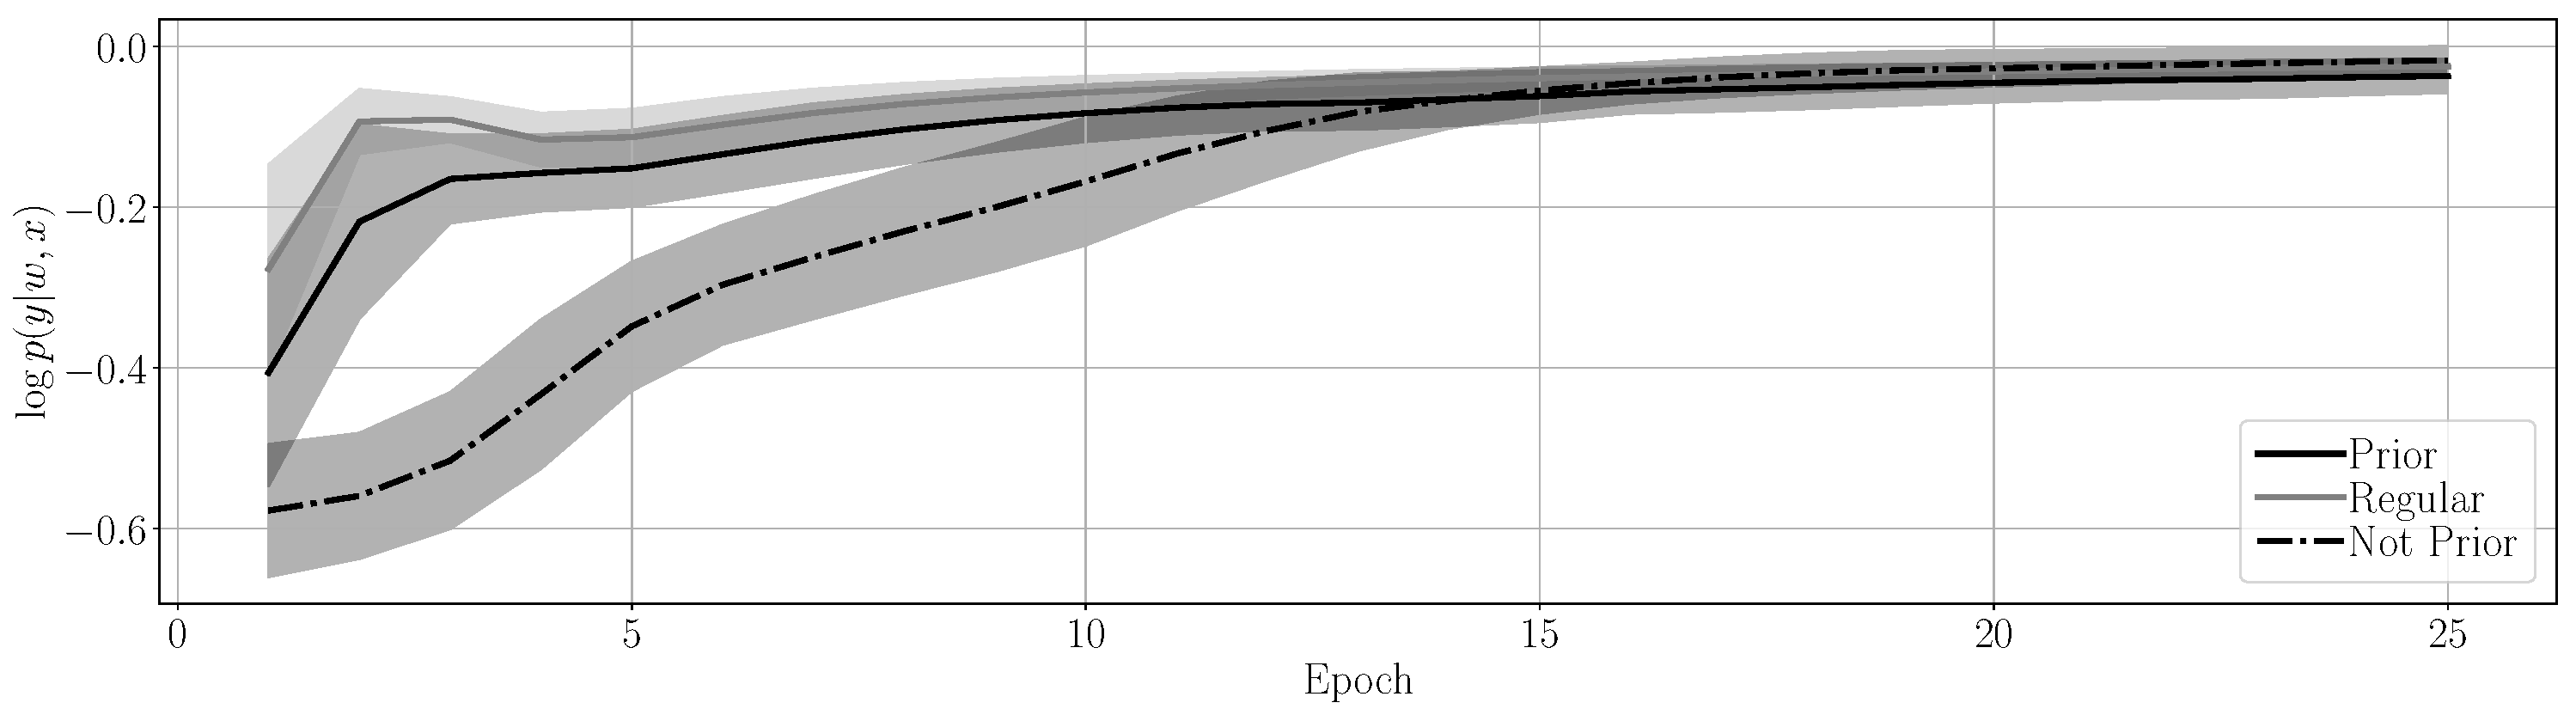
\includegraphics[width=1\textwidth]{results/priorexpert/experiment_synt_likelihood_progress}
\caption{График зависимости логарифма правдоподобия \eqref{eq:st:new:1} от номера итерации.}
\label{experiment:st:2:2}
\end{figure}

\begin{figure}[h!t]\center
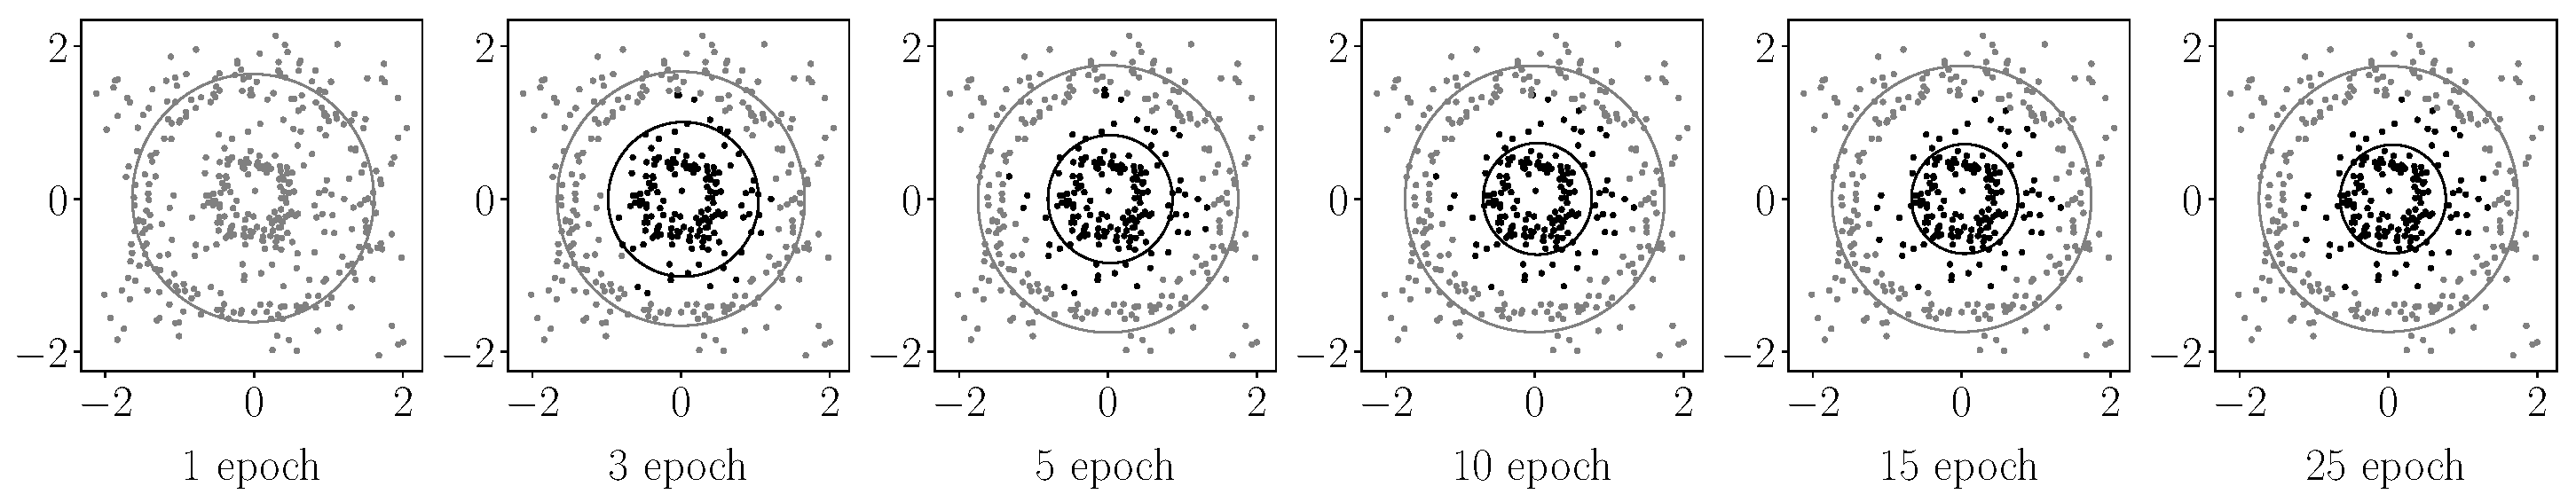
\includegraphics[width=1\textwidth]{results/priorexpert/experiment_synt_regular_progress}
\caption{Визуализации процесса сходимости мультимодели с использованием априорной регуляриции.}
\label{experiment:st:2:3}
\end{figure}

\begin{figure}[h!t]\center
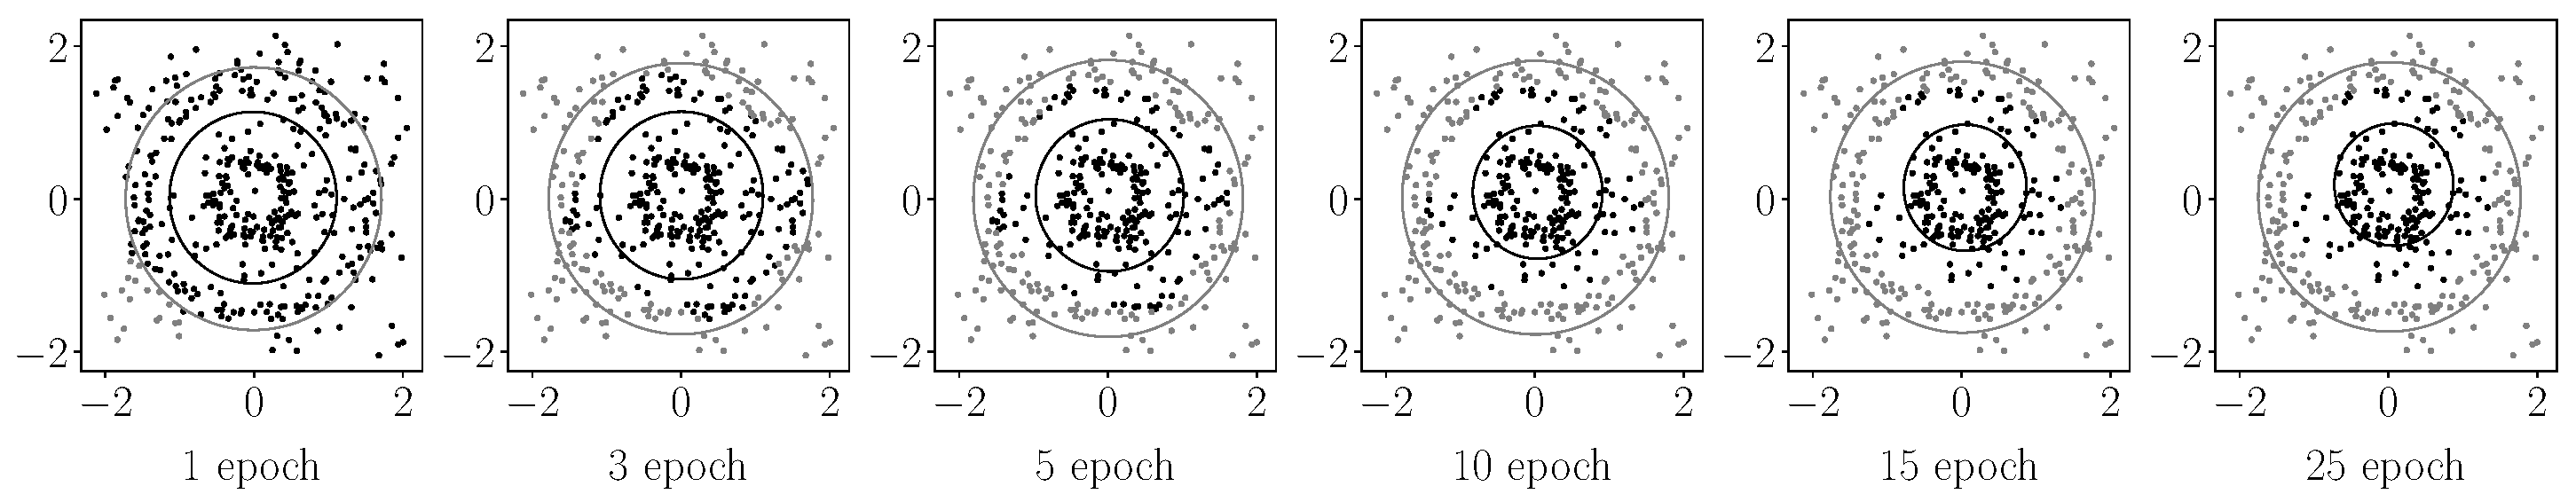
\includegraphics[width=1\textwidth]{results/priorexpert/experiment_synt_prior_progress}
\caption{Визуализации процесса сходимости мультимодели с использованием априорного распределением.}
\label{experiment:st:2:4}
\end{figure}

\begin{figure}[h!t]\center
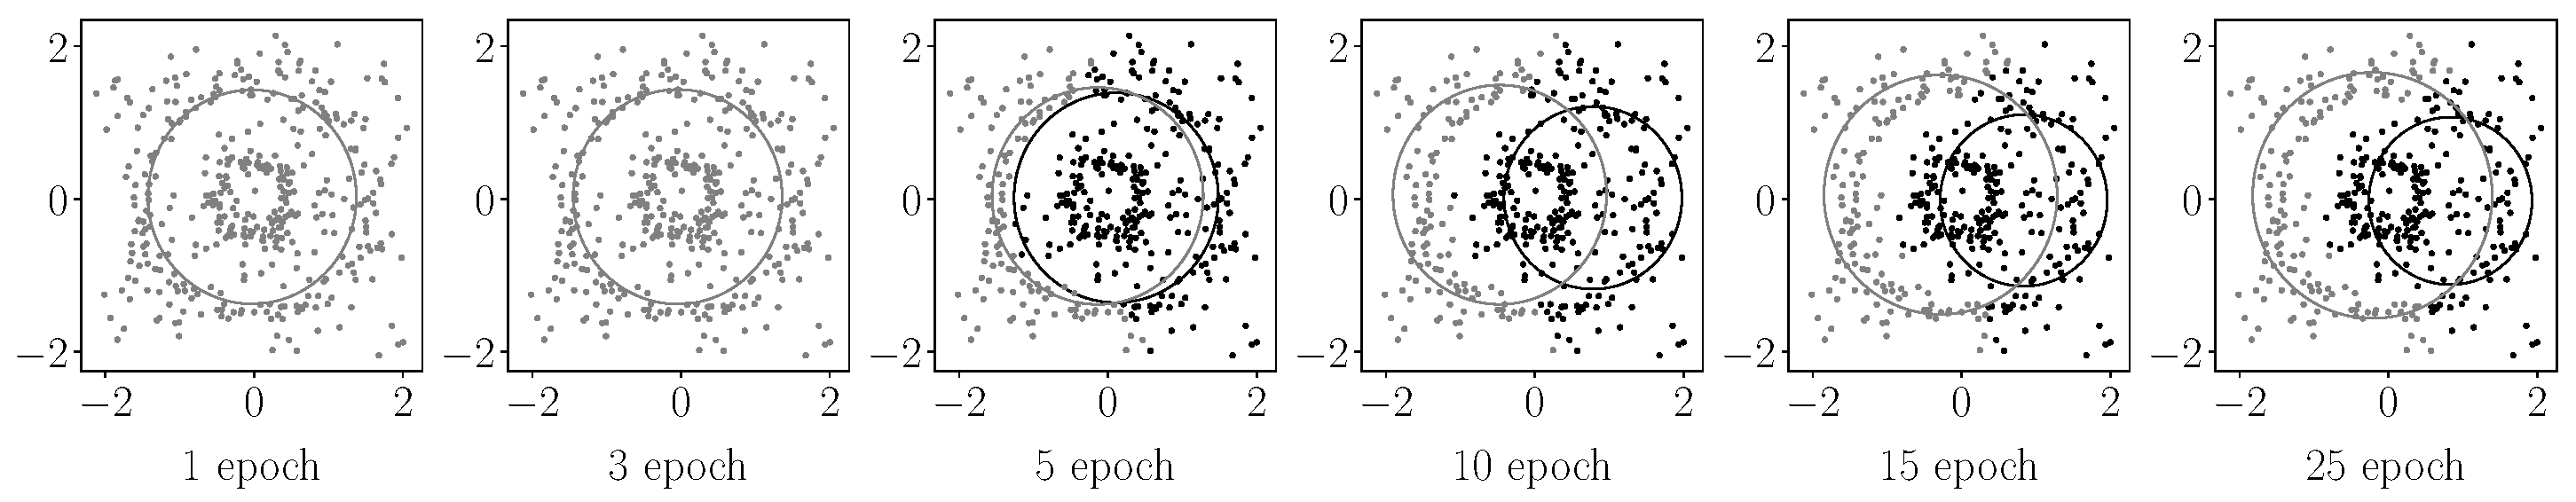
\includegraphics[width=1\textwidth]{results/priorexpert/experiment_synt_not_prior_progress}
\caption{Визуализации процесса сходимости мультимодели без использования априорного распределения.}
\label{experiment:st:2:5}
\end{figure}
Данная часть эксперимента анализирует качество сходимости ЕМ-алгоритма для разных мультимоделей $\textbf{f}_1, \textbf{f}_2, \textbf{f}_3$.
Анализ всех мультимоделей проводиться на выборке Synthetic 3.

На рис. \ref{experiment:st:2:1} показана зависимость предсказано центра и радуса в зависимости от номера итерации ЕМ-алгоритма.
Мультимодель $\textbf{f}_2,$ которая использует априорное распределение аппроксимирует окружность лучше мультимодели $\textbf{f}_1,$ которая не использует никакого априорного распределения.
Мультимодель $\textbf{f}_3,$ которая использует регуляризатор априорных распределений является более стабильной, чем мультимодель $\textbf{f}_2$.

На рис. \ref{experiment:st:2:2} показана зависимость логарифма правдоподобия \eqref{eq:st:new:1} от номера итерации EM-алгоритма.
Логарифм правдоподобия мультимодели $\textbf{f}_2, \textbf{f}_3$ растет быстрее чем логарифм правдоподобия мультимодели $\textbf{f}_1$.  После $20$-й итерации все мультимодели имеют одинаковое правдоподобие.

На рис. \ref{experiment:st:2:3}-\ref{experiment:st:2:5} показан процесс сходимости для разных мультимоделей $\textbf{f}_1, \textbf{f}_2, \textbf{f}_3$.
На рис. \ref{experiment:st:2:5} показана мультимодель $\textbf{f}_1$, которая аппроксимирует окружности не верно.
На рис. \ref{experiment:st:2:3}-\ref{experiment:st:2:4} показаны мультимодели $\textbf{f}_2, \textbf{f}_3$, которые аппроксимируют окружности верно.

Вычислительный эксперимент показывает, что мультимодели $\textbf{f}_2, \textbf{f}_3,$ которые используют априорные распределения на параметры экспертов аппроксимируют окружности лучше чем мультимодель $\textbf{f}_1,$ которая работает без априорных распределений.


\paragraph{Анализ мультимоделей в зависимости от уровня шума.} 
\begin{figure}[h!t]\center
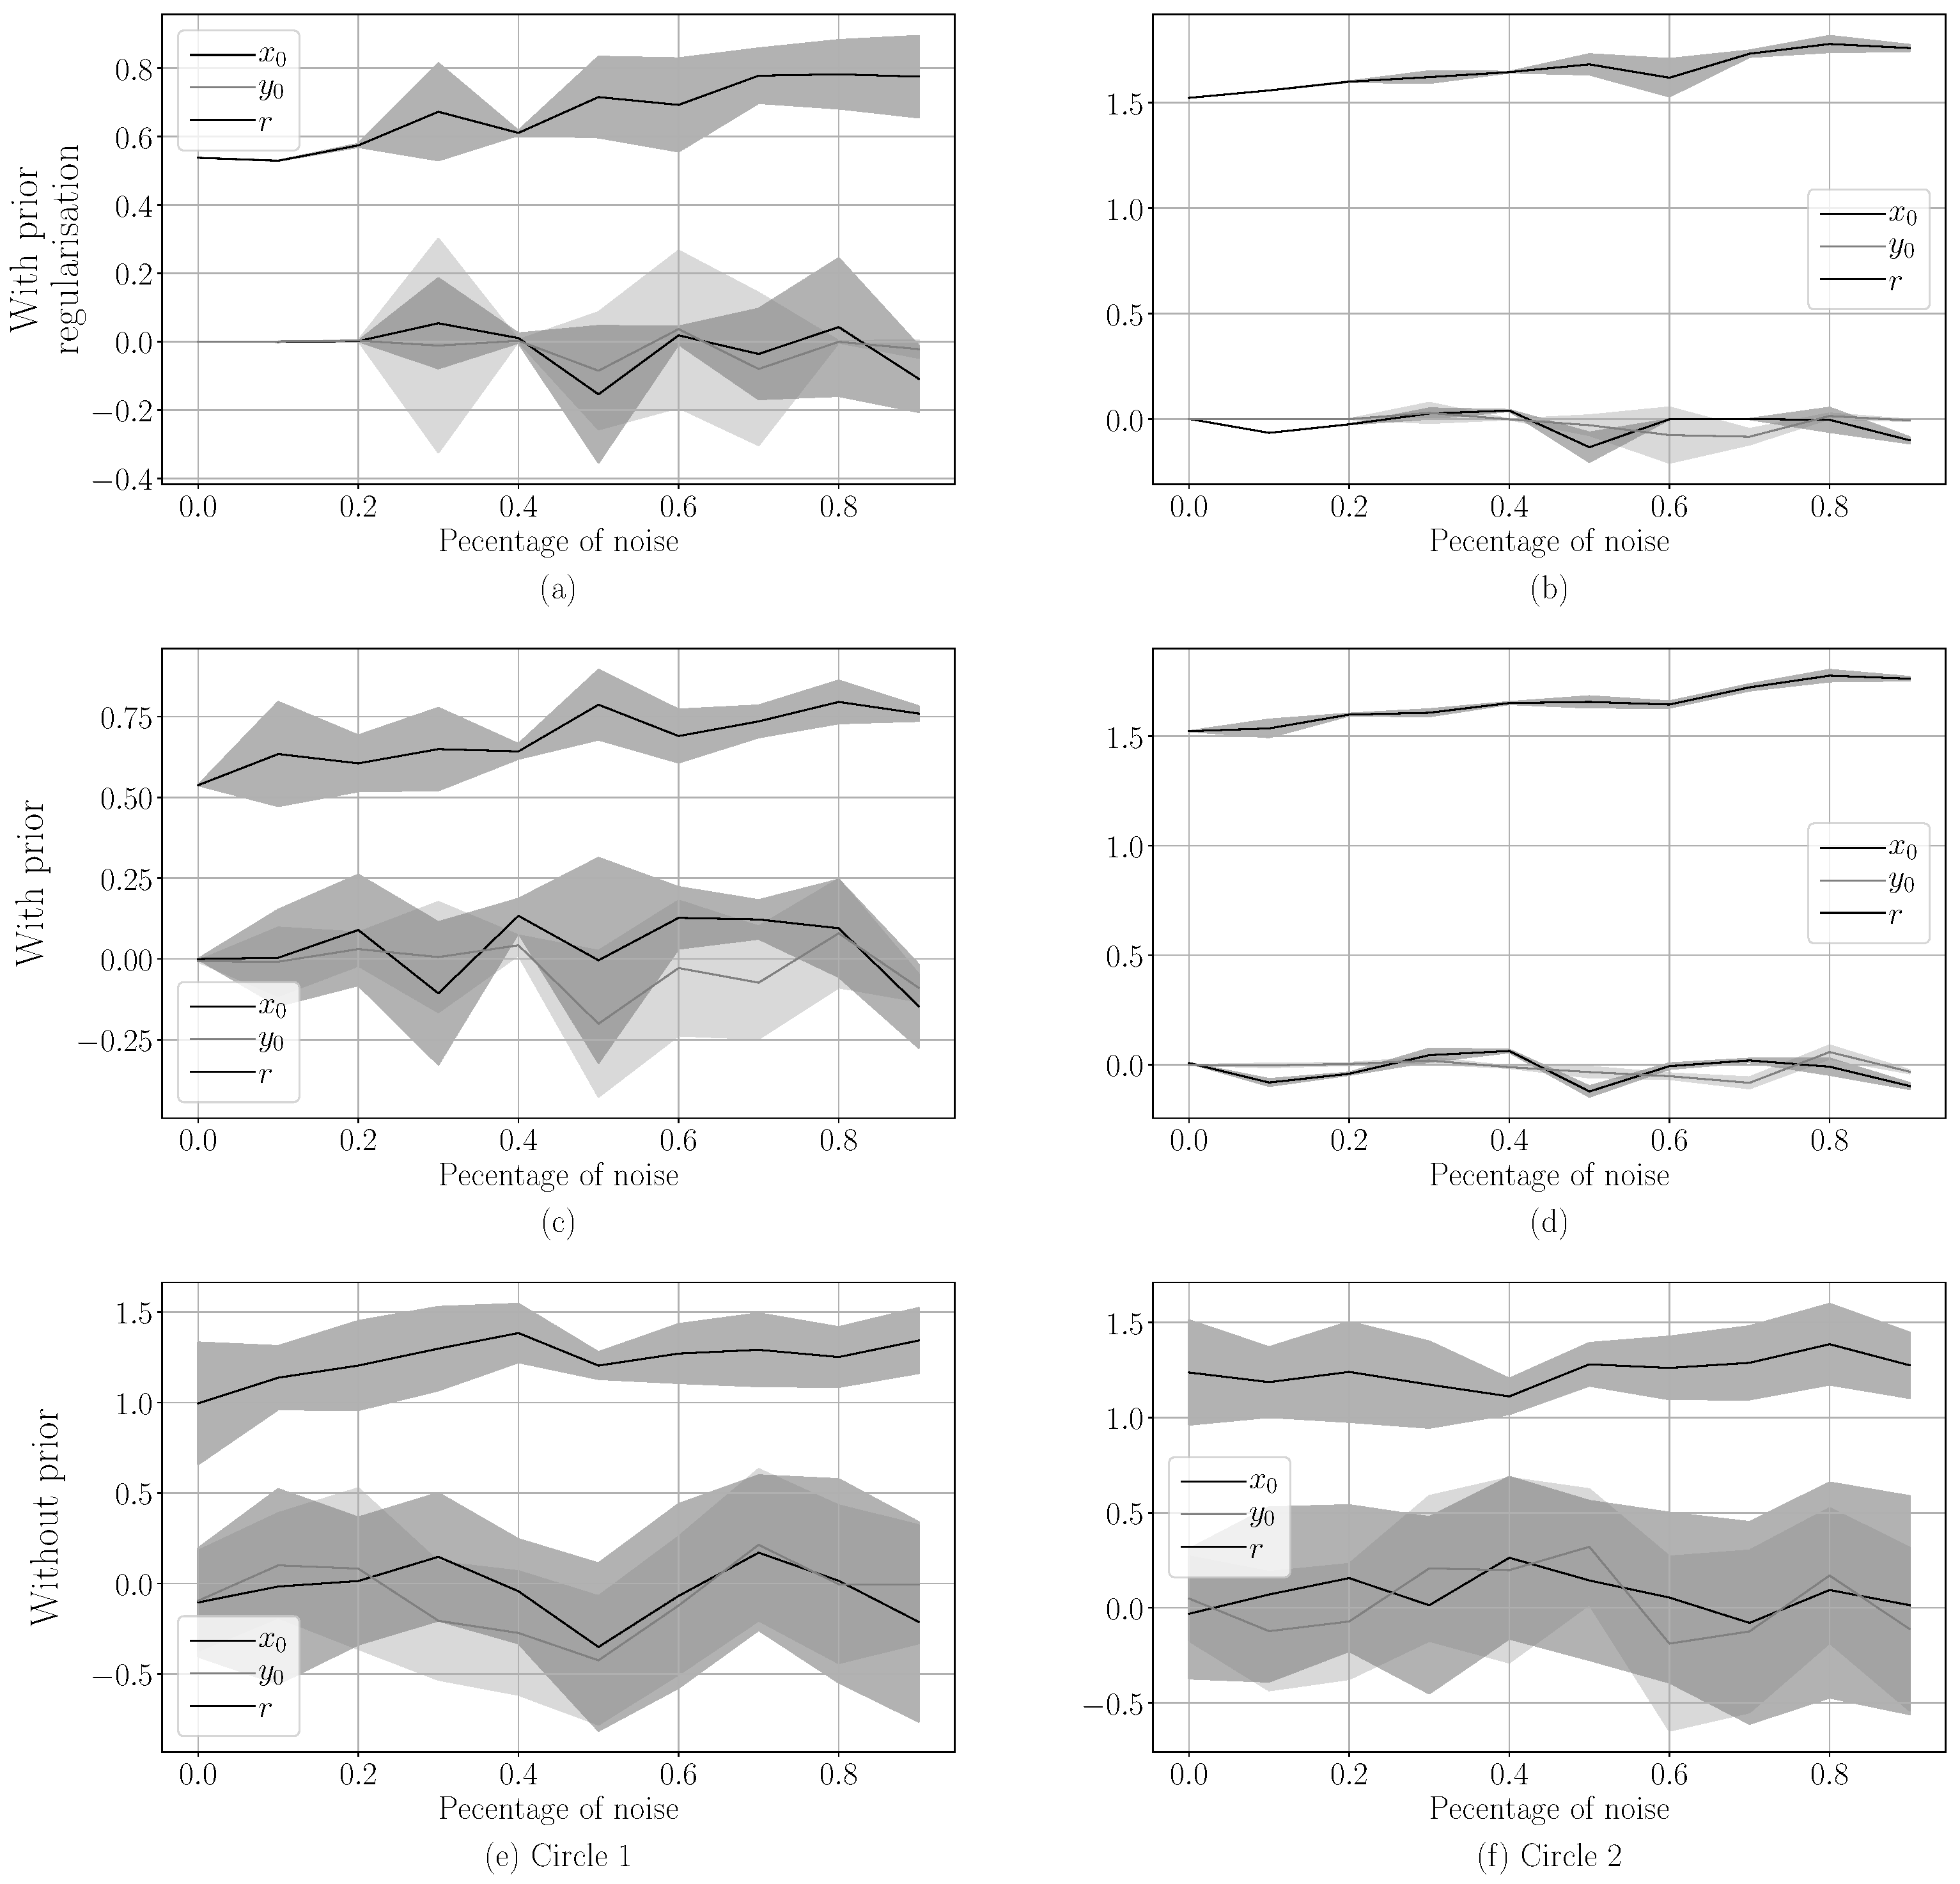
\includegraphics[width=1\textwidth]{results/priorexpert/experiment_synthetic_param_progress_noise}
\caption{рафик зависимости центра и радиуса окружностей от номера итерации: (a)--(b) модель с регуляризацией априорных распределений; (c)--(d) модель с заданными априорными распределениями на параметры моделей; (e)--(f) модель без задания априорных распределений}
\label{experiment:st:3:1}
\end{figure}

\begin{figure}[h!t]\center
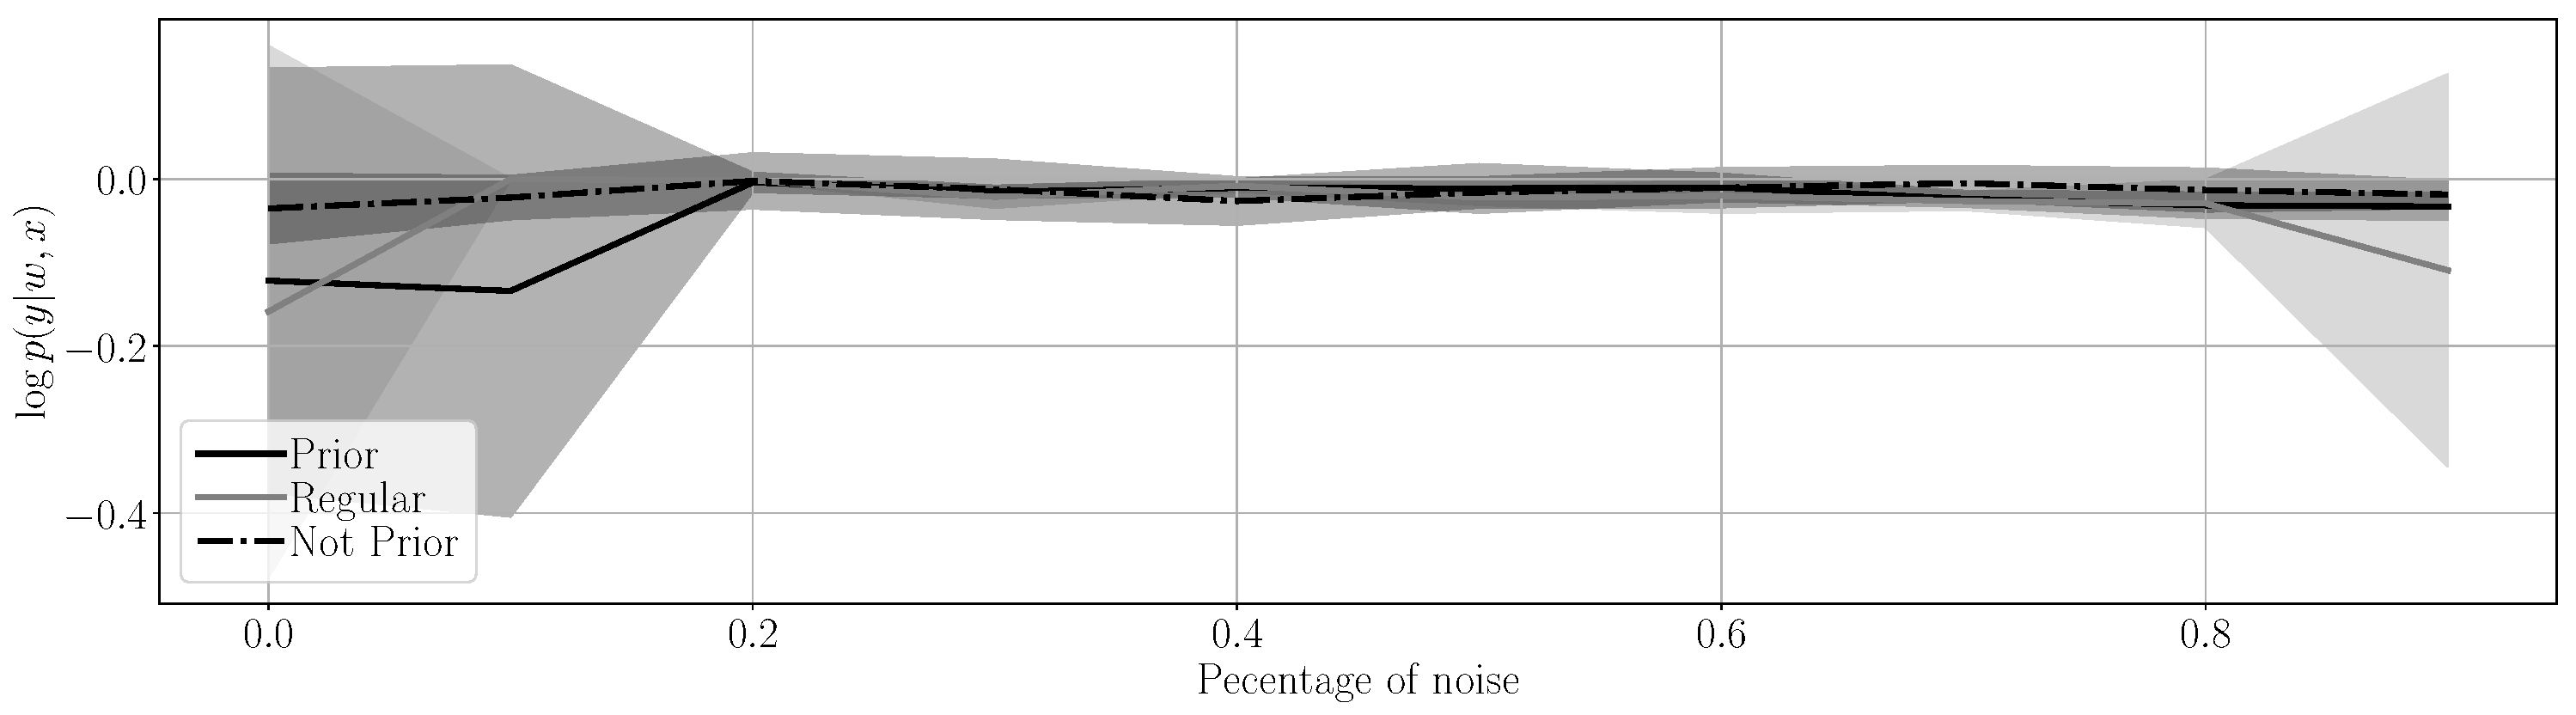
\includegraphics[width=1\textwidth]{results/priorexpert/experiment_synt_likelihood_progress_noise}
\caption{График зависимости логарифма правдоподобия \eqref{eq:st:new:1} от уровня шума.}
\label{experiment:st:3:2}
\end{figure}

Данная часть эксперимента анализирует зависимость разных мультимоделей $\textbf{f}_1, \textbf{f}_2, \textbf{f}_3$ от уровня шума. 
Анализ всех мультимоделей проводиться на выборке Synthetic 1, с добавлением разного уровня шума.
Минимальный уровень шума равен $0$, когда числа шумовых точек равно $0$. Максимальный уровень шума равен $1$, когда число шумовых точек равно числу точек на изображении.
На рис. \ref{experiment:st:3:1} показан график зависимости центра окружности и ее радиус в зависимости от уровня шума. Из графика видно, что радиус окружности увеличивается при увеличении уровня шума. 
Мультимодели $\textbf{f}_2, \textbf{f}_3$ аппроксимируют центр окружности верно, но мультимодель $\textbf{f}_3$ более устойчива к шуму .
На рис. \ref{experiment:st:3:2} показана зависимость логарифма правдоподобия \eqref{eq:st:new:1} от уровня шума. 
Из графика видно, что логарифм правдоподобия \eqref{eq:st:new:1} эквивалентный для всех мультимоделей, но на рис. \ref{experiment:st:3:1} видно, что качество аппроксимации \eqref{eq:ce:ex:0:1} зависит от мультимодели.
Данная часть вычислительного эксперимента показывает, что мультимодель $\textbf{f}_3$ с регуляризацией априорного распределения является более устойчива к шуму, чем остальные.

\paragraph{Реальные данные.}
\begin{figure}[h!t]\center
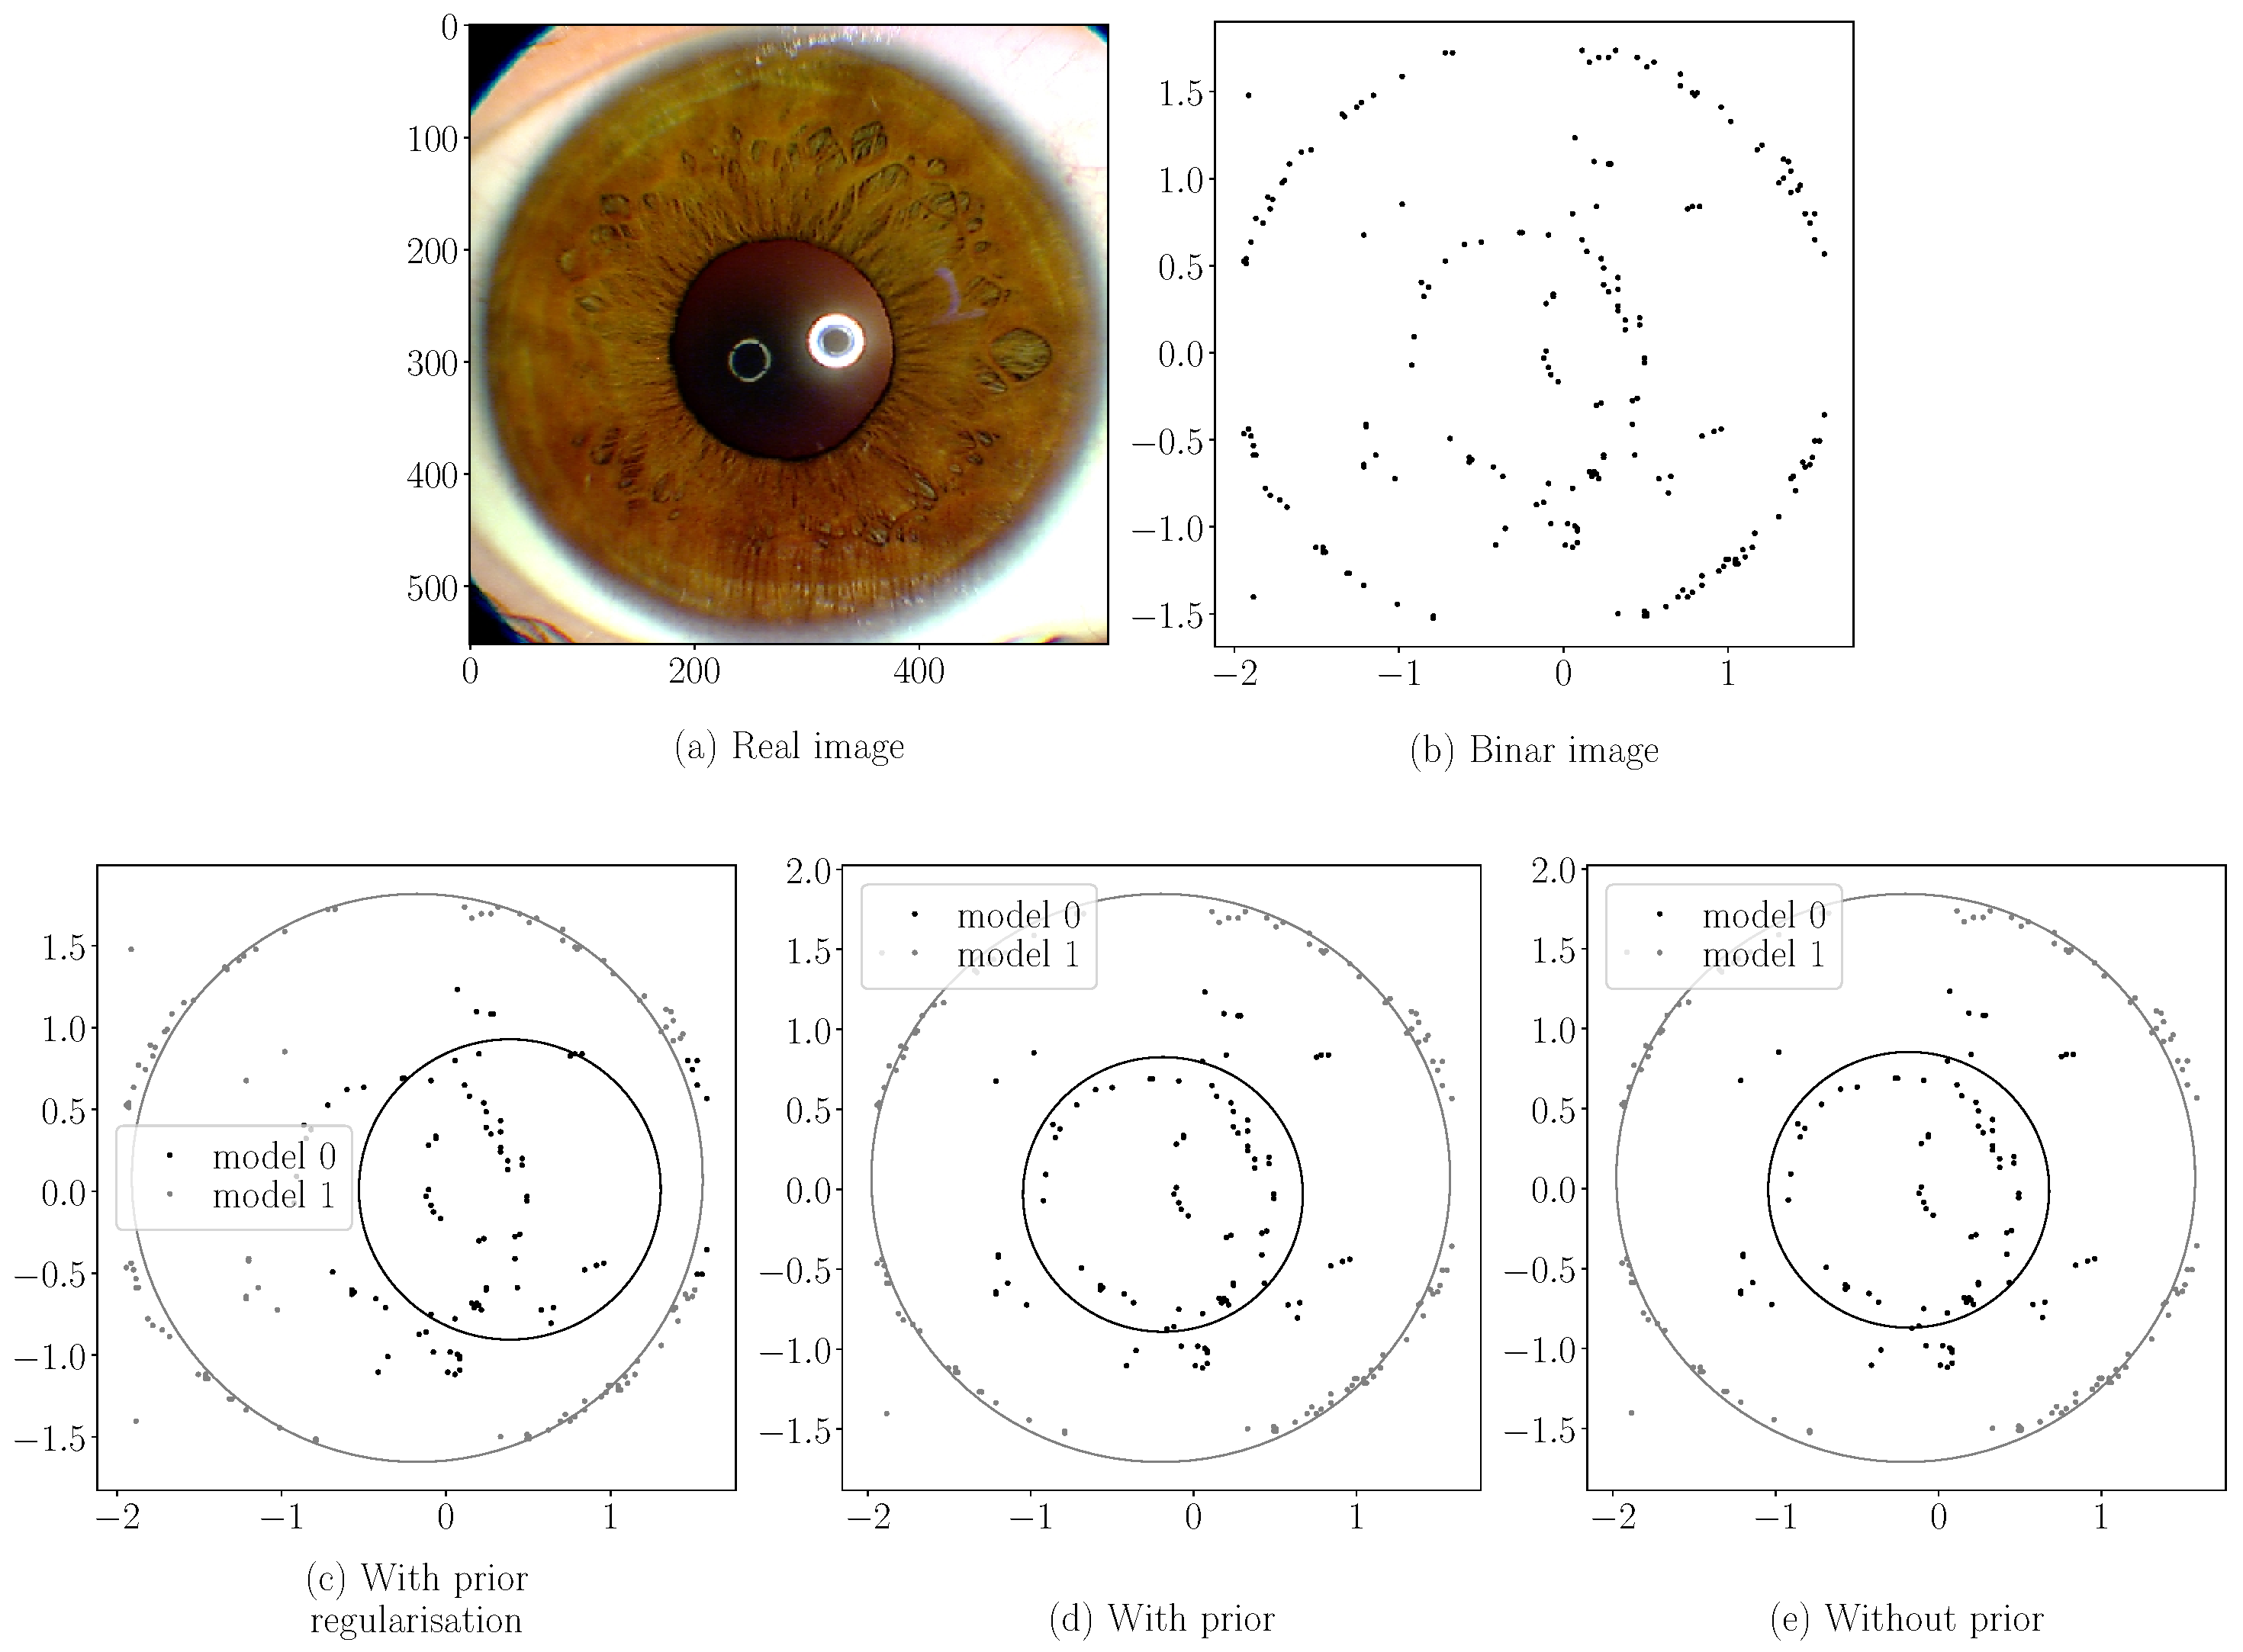
\includegraphics[width=0.9\textwidth]{results/priorexpert/experiment_real_compare}
\caption{Мультимодель в зависимости от разных априорных предположений на реальном изображении: (a) исходное изображение; (b) бинаризованое изображение; (c) мультимодель без априорных предположений; (d) мультимодель с априорными распределениями на параметрах локальных моделей; (e) мультимодель с регуляризаций на априорных распределениях параметров локальных моделей.}
\label{experiment:2}
\end{figure}

Данная часть эксперимента анализирует разные мультимодели $\textbf{f}_1, \textbf{f}_2, \textbf{f}_3$ на реальной выборке.
На рис. \ref{experiment:2} показан результат работы разных мультимоделей.
Мультимодель $\textbf{f}_1$  не верно аппроксимирует меньшую окружность.
Мультимодели $\textbf{f}_2, \textbf{f}_3$ аппроксимируют обе окружности верно.

\begin{figure}[h!t]\center
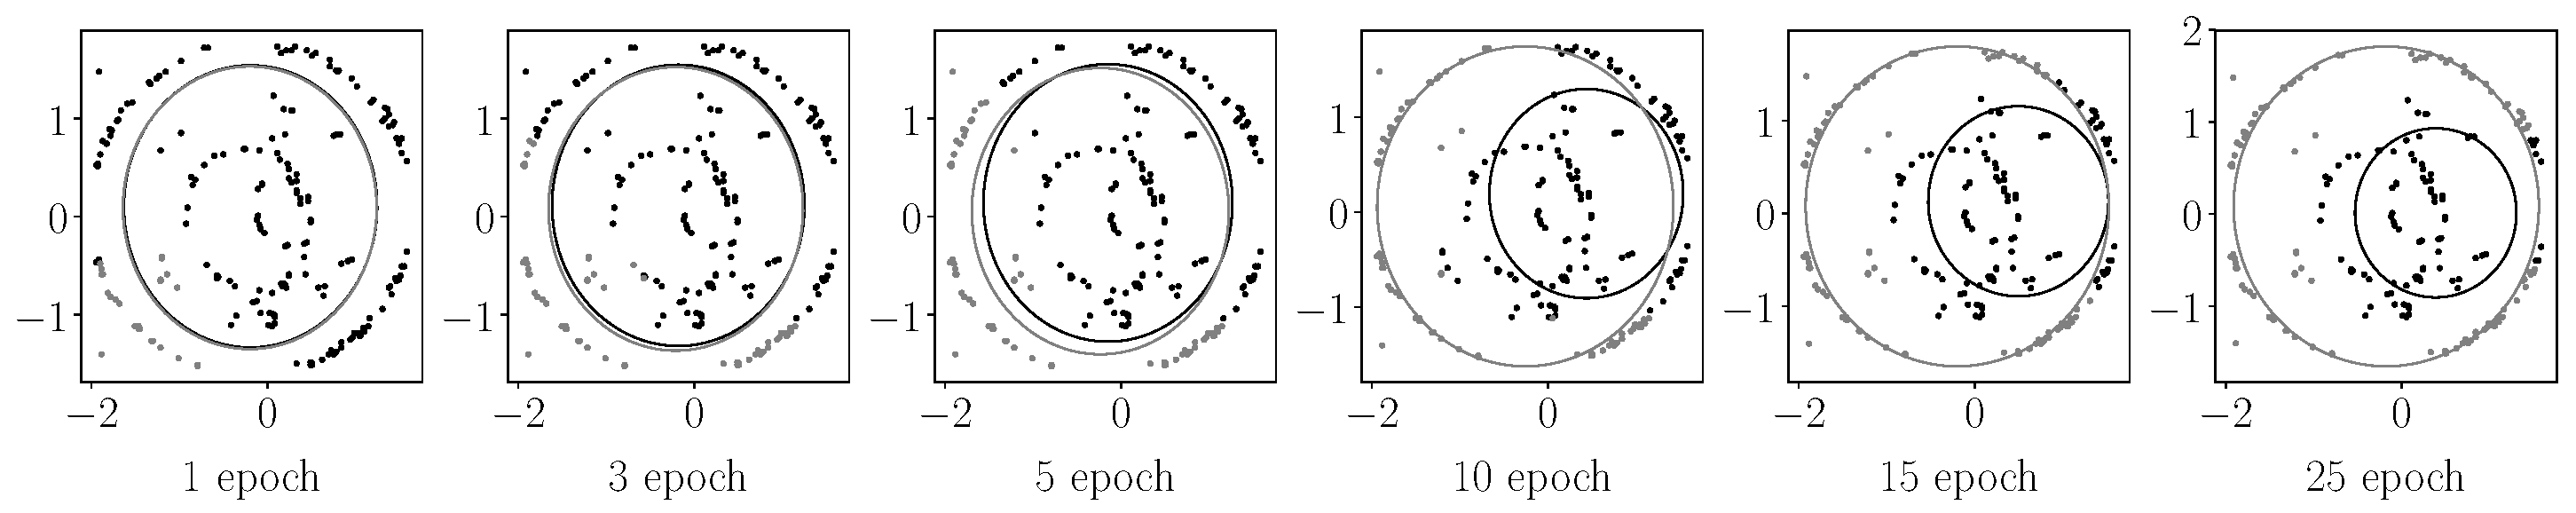
\includegraphics[width=1\textwidth]{results/priorexpert/experiment_real_not_prior}
\caption{Визуализации процесса сходимости мультимодели без использования априорного распределения.}
\label{experiment:3}
\end{figure}

\begin{figure}[h!t]\center
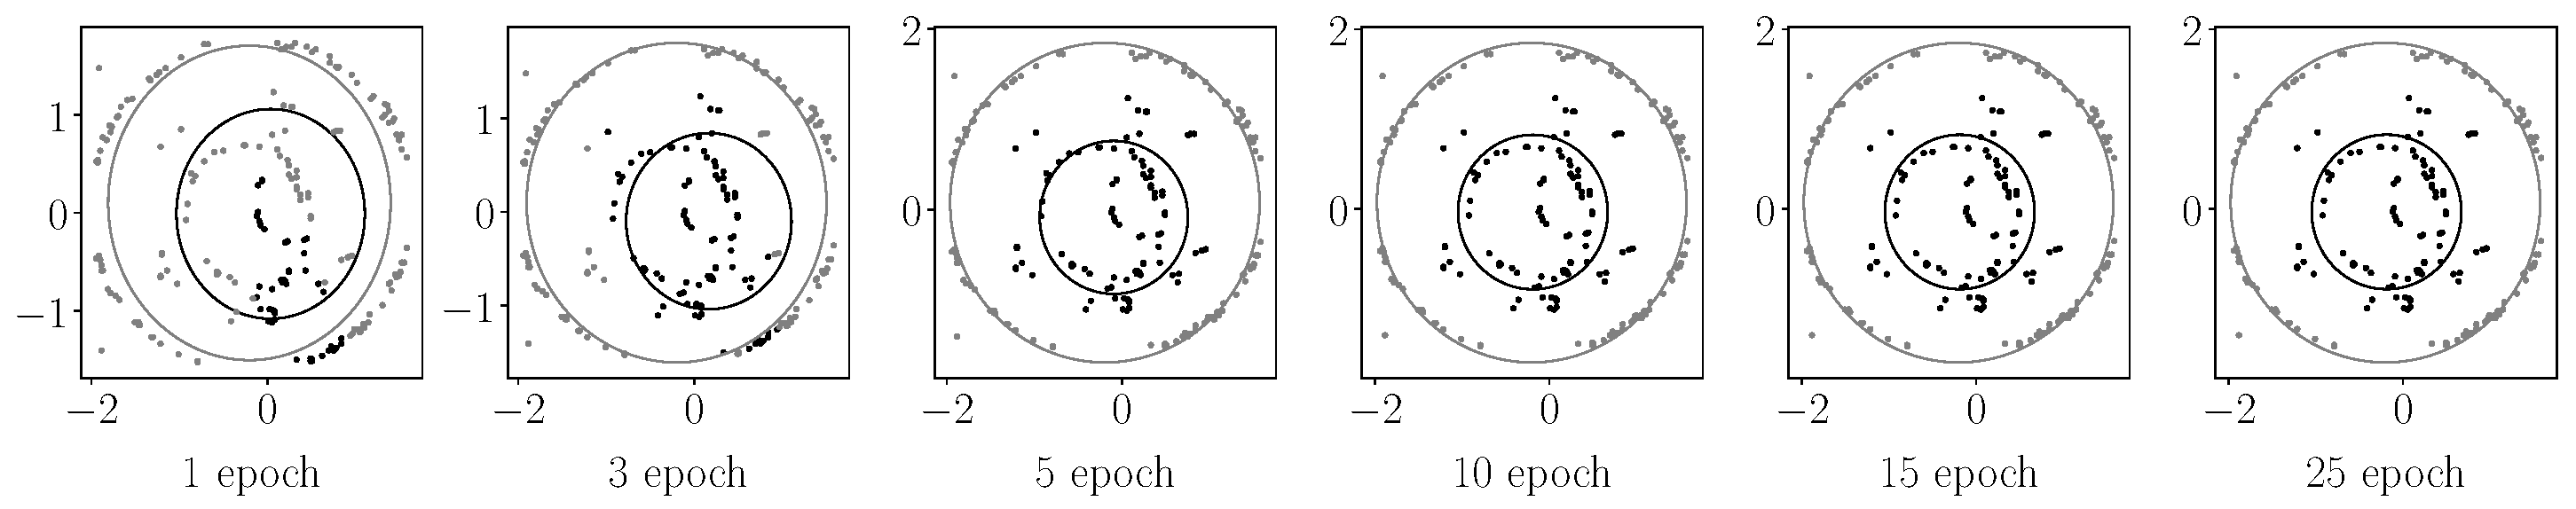
\includegraphics[width=1\textwidth]{results/priorexpert/experiment_real_prior}
\caption{Визуализации процесса сходимости мультимодели с использованием априорного распределением.}
\label{experiment:4}
\end{figure}

\begin{figure}[h!t]\center
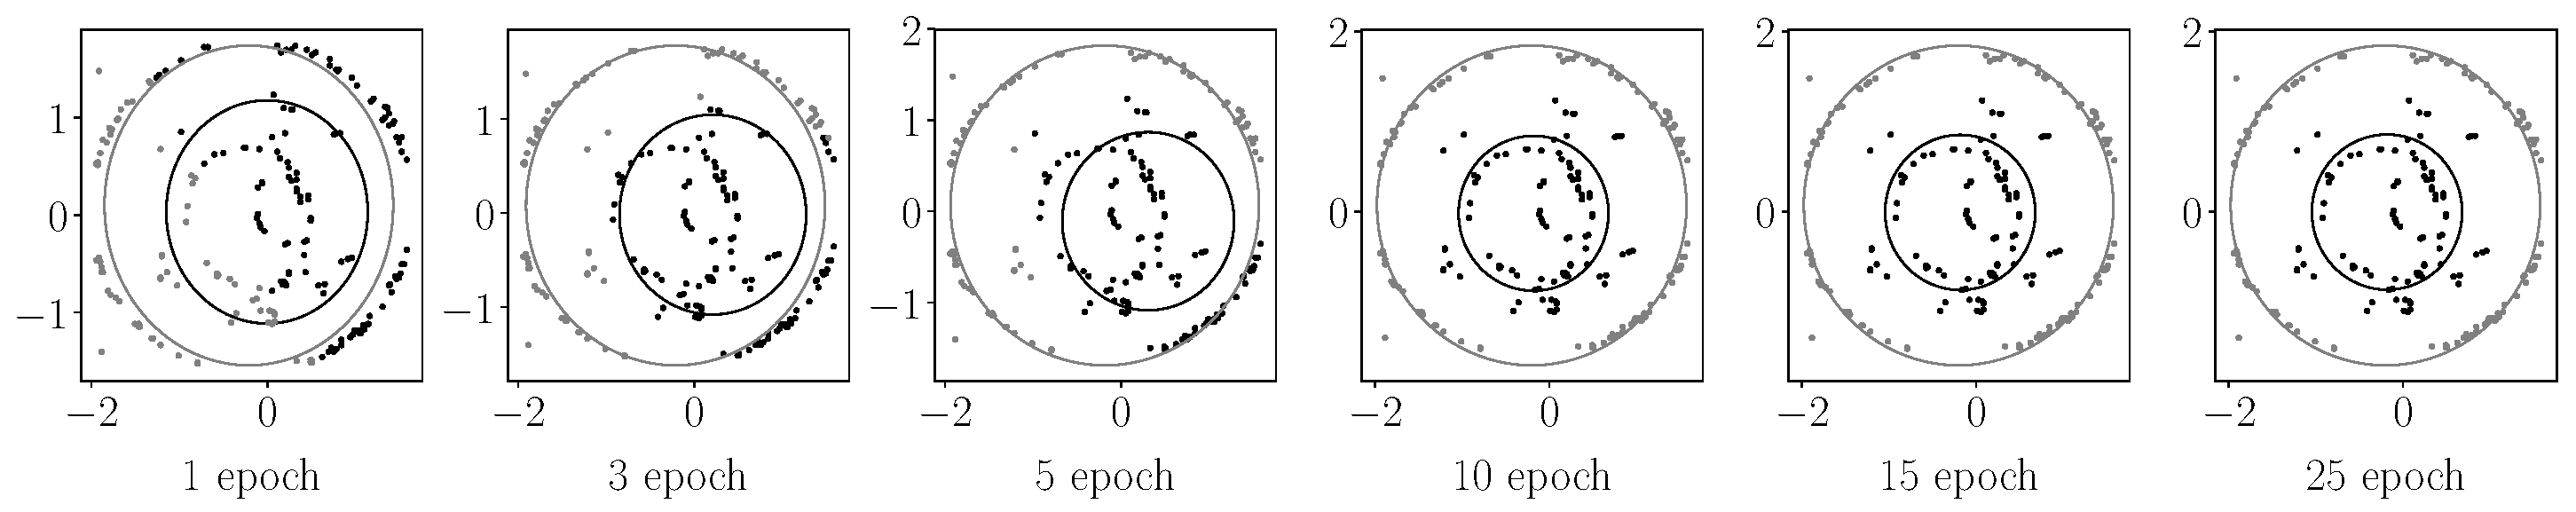
\includegraphics[width=1\textwidth]{results/priorexpert/experiment_real_regular}
\caption{Визуализации процесса сходимости мультимодели с использованием априорной регуляриции.}
\label{experiment:5}
\end{figure}

На рис. \ref{experiment:3}-\ref{experiment:5} показан процесс аппроксимации для разных мультимоделей $\textbf{f}_1, \textbf{f}_2, \textbf{f}_3$.

Данная часть эксперимента показывает, что мультимодели $\textbf{f}_2, \textbf{f}_3$ аппроксимируют окружности на реальных изображениях лучше, чем мультимодель $\textbf{f}_1$.
\newpage


\section{Модели привилегированного обучения и дистиляции}
Повышение точности аппроксимации в задачах машинного обучения влечет за собой повышение сложности моделей и как следствие снижает их интерпретируемость. Примером такого усложнения являются следующие модели: трансформеры \cite{Vaswani2017}, BERT \cite{Devlin2018}, ResNet \cite{Kaiming2015} а также ансамбли этих моделей. 

При построении модели машинного обучения используется два свойства: сложность модели и точность аппроксимации модели. Сложность влияет на время, которое модель требуется для принятия решения, а также на интерпретируемость модели, следовательно модель которая имеют меньшую сложность является более предпочтительной \cite{bachteev2018}. С другой стороны точность аппроксимации модели нужно максимизировать. В данной работе рассматривается метод \textit{дистилляции} модели. Данные метод позволяет строить новые модели на основе ранее обученых моделей.

\begin{definition}
Дистилляция модели --- уменьшение сложности модели путем выбора модели в множестве более простых моделей с использованием ответов более сложной модели.
\end{definition}

В работе \cite{Hinton2015} Дж.\,Е. Хинтоном рассматривается метод дистилляции моделей машинного обучения для задачи классификации. В работе проведен ряд экспериментов, в которых проводилась дистилляции моделей для разных задач машинного обучения. Эксперимент на выборке MNIST \cite{mnist}, в котором избыточно сложно нейросеть была дистиллирована в нейросеть меньшей сложности. Эксперимент по Speech Recognition, в котором ансамбль моделей был \textit{дистиллирован} в одну модель. Также в работе \cite{Hinton2015} был проведен эксперимент по обучению экспертных моделей на основе одной большой модели.

\begin{definition}
Привилегированная информация --- множество признаков, которые доступны только в момент выбора модели, но не в момент тестирования.
\end{definition}

В работе \cite{Vapnik2015} В.\,Н. Вапником введено понятия \textit{привилегированной информации}. В работе \cite{Lopez2016} метод дистилляции \cite{Hinton2015} используется вместе с привилегированным обучениям \cite{Vapnik2015}. В предложенном методе на первом этапе обучается модель \textit{учителя} в пространстве привилегированной информации, после чего обучается модель \textit{ученика} в исходном признаковом пространстве используя \textit{дистилляцию} \cite{Hinton2015}. Для обучения строится функция ошибки специального вида, анализируемая в данной работе. Эта функция состоит из нескольких слагаемых, включая ошибки учителя, ученика и регуляризирующие элементы.  Первые варианты подобной функции ошибки были предложены А.\,Г. Ивахненко \cite{Ivakhnenko1994}.

\begin{definition}
Учитель --- фиксируемая модель, ответы которой используются при выборе модели ученика.
\end{definition}

\begin{definition}
Ученик --- модель, которая выбирается согласно какого-либо критерия.
\end{definition}

В данной работе предлагается рассмотреть вероятностный подход к решению задачи дистилляции модели и задачи привилегированного обучения. Подход обобщается на случай, когда привилегированная информация доступна не для всех объектов из обучающей выборки. В рамках вероятностного подхода предлагается анализ и обобщение функции ошибки \cite{Hinton2015, Lopez2016}. Рассматриваются частные задачи классификации и регрессии \cite{Ivakhnenko1994}.


В рамках вычислительного эксперимента анализируются методы использующие и не использующие модель учителя при обучение модели ученика. Для анализа используются реальные выборки для задачи классификации изображений FashionMNIST \cite{fashionmnist} и для задачи классификации текстов Twitter Sentiment Analysis \cite{twiter2013}. Выборка FashionMNIST использовалась вместо общепринятой выборки MNIST, так как последняя имеет приемлемое качество аппроксимации даже для линейного классификатора. Вычислительный эксперимент использует модели разной сложности: линейная модель, полносвязная нейронная сеть, сверточная нейронная сеть \cite{LeCun1989}, модель Bi-LSTM \cite{Schmidhuber1997} и модель BERT \cite{Devlin2018}.

\subsection{Постановка задачи обучения с учителем: Хинтона и Вапника}
Задано множество объектов $\bm{\Omega}$ и множество целевых переменных $\mathbb{Y}$. Множество $\mathbb{Y}=\{1,\cdots,K\}$ для задачи классификации, где $K$ число классов, множество $\mathbb{Y}=\mathbb{R}$ для задачи регрессии.
Для каждого объекта из $\omega_i \in \bm{\Omega}$ задана целевая переменная $\mathbf{y}_i = \mathbf{y}\bigr(\omega_i\bigr)$. Множество целевых переменных для всех объектов обозначим $\mathbf{Y}$.
Для множества $\bm{\Omega}$ задано отображение в некоторое признаковое пространство $\mathbb{R}^{n}$:
\[
\label{eq:st:phi}
\begin{aligned}
\varphi:\bm{\Omega} \to \mathbb{R}^{n}, \quad \left|\bm{\Omega}\right| = m,
\end{aligned}
\]
где $n$ размерность признакового пространства, а $m$ количество объектов в множестве $\bm{\Omega}$. Отображение $\varphi$ отображает объект $\omega_i \in \bm{\Omega}$ в соответствующий ему вектор признаков $\mathbf{x}_i = \varphi(\omega_i)$.
Пусть для объектов $\bm{\Omega}^* \subset \bm{\Omega}$ задана привилегированная информация:
\[
\label{eq:st:phi*}
\begin{aligned}
\varphi^*:\bm{\Omega}^* \to \mathbb{R}^{n^*}, \quad \left|\bm{\Omega}^*\right| = m^*,
\end{aligned}
\]
где $m^* \leq m$ --- число объектов с привилегированной информацией, $n^*$ --- число признаков в пространстве привилегированной информации. Отображение $\varphi^*$ отображает объект $\omega_i \in \bm{\Omega^*}$ в соответствующий ему вектор признаков $\mathbf{x}^*_i = \varphi^*(\omega_i)$.

Множество индексов объектов, для которых известна привилегированная информация, обозначим $\mathcal{I}$:
\[
\label{eq:st:3}
\begin{aligned}
\mathcal{I} = \{1 \leq i \leq m | \text{для $i$-го объекта задана привилегированная информация}\},
\end{aligned}
\]
а множество индексов объектов, для которых не известна привилегированная информация, обозначим $\{1, \cdots, m\}\setminus \mathcal{I} = \bar{\mathcal{I}}$.

Пусть на множестве привилегированных признаков задана функция учителя $\mathbf{f}\bigr(\mathbf{x}^*\bigr)$:
\[
\label{eq:st:4}
\begin{aligned}
\mathbf{f}:\mathbb{R}^{n^*} \to \mathbb{Y}^*,
\end{aligned}
\]
где $\mathbb{Y}^*=\mathbb{Y}$ для задачи регрессии и $\mathbb{Y}^*$ является единичным симплексом $\mathcal{S}_K$ в пространстве размерности $K$ для задачи классификации. Модель учителя $\mathbf{f}$ ставит объекты $\mathbf{X}^*$ в соответствие объектам $\mathbf{S},$ то есть  $\mathbf{f}\bigr(\mathbf{x}^*_i\bigr)=\mathbf{s}_i$.

Требуется выбрать модель ученика $\mathbf{g}\bigr(\mathbf{x}\bigr)$ из множества:
\[
\label{eq:st:G}
\begin{aligned}
\mathfrak{G} = \left\{\mathbf{g}| \mathbf{g}:\mathbb{R}^{n} \to \mathbb{Y}^*\right\},
\end{aligned}
\]
например для задачи классификации множество $\mathfrak{G}$ может быть параметрическим семейством функций линейных моделей:
\[
\label{eq:st:G:lin:cl}
\begin{aligned}
\mathfrak{G}_\text{lin,cl} = \left\{\mathbf{g}\bigr(\mathbf{W}, \mathbf{x}\bigr)| \mathbf{g}\bigr(\mathbf{W}, \mathbf{x}\bigr) = \textbf{softmax}\bigr(\mathbf{W}\mathbf{x}\bigr), \quad \mathbf{W} \in \mathbb{R}^{n\times K}\right\}.
\end{aligned}
\]

Рассмотрим описание метода предложеного в работах \cite{Hinton2015, Lopez2016}. В рамках данных работ предполагается, что для всех данных доступна привилегированная информация $\mathcal{I} = \{1, 2, \cdots, m\}$. В работе \cite{Hinton2015} решается задача классификации вида:
\[
    \mathfrak{D} = \{\left(\mathbf{x}_i, y_i\right)\}_{i=1}^{m}, \qquad \mathbf{x}_i \in \mathbb{R}^{n}, \quad y_i \in \mathbb{Y}=\{1, \cdots, K\},
\]
где $y_i$ --- это класс объекта, также будем обозначать $\mathbf{y}_i$ вектором вероятности для класса $y_i$.

В постановке Хинтона рассматривается параметрическое семейство функций:
\[
\label{eq:G:set:cl}
\mathfrak{G}_{\text{cl}} = \left\{\mathbf{g}| \mathbf{g} = \text{softmax}\bigr(\mathbf{z}\bigr(\mathbf{x}\bigr)/T\bigr), \quad \mathbf{z}: \mathbb{R}^n \to \mathbb{R}^K \right\},
\]
где $\mathbf{z}$ --- это дифференцируемая параметрическая функция заданной структуры, $T$ --- параметр температуры. В качестве модели учителя $\mathbf{f}$ рассматривается функция из множества $\mathfrak{F}_{\text{cl}}$:
\[
\label{eq:F:set:cl}
\mathfrak{F}_{\text{cl}} = \left\{\mathbf{f}| \mathbf{f} = \text{softmax}\bigr(\mathbf{v}\bigr(\mathbf{x}\bigr)/T\bigr), \quad \mathbf{v}: \mathbb{R}^n \to \mathbb{R}^K \right\},
\]
где $\mathbf{v}$ --- это дифференцируемая параметрическая функция заданной структуры, $T$ --- параметр температуры.
Параметр температуры $T$ имеет следующие свойства:
\begin{enumerate}
    \item при $T\to 0$ получаем вектор, в котором один из классов имеет единичную вероятность;
    \item при $T\to \infty$ получаем равновероятные классы.
\end{enumerate}

Функция потерь $\mathcal{L}$ в которой учитывается перенос информации от модели учителя $\mathbf{f}$ к модели ученика $\mathbf{g}$ имеет следующий вид:
\[
\label{eq:hinton:1}
\begin{aligned}
   \mathcal{L}_{st}\bigr(\mathbf{g}\bigr) = &-\sum_{i=1}^{m}\underbrace{{\sum_{k=1}^{K}y^k_i\log\mathbf{g}\bigr(\mathbf{x}_i\bigr)\bigr|_{T=1}}}_{\text{исходная функция потерь}}\\
   &-\sum_{i=1}^{m}\underbrace{{\sum_{k=1}^{K}\mathbf{f}\bigr(\mathbf{x}_i\bigr)\bigr|_{T=T_0}\log\mathbf{g}\bigr(\mathbf{x}_i\bigr)\bigr|_{T=T_0}}}_{\text{слагаемое дистилляция}},
\end{aligned}
\]
где $\cdot\bigr|_{T=t}$ обозначает, что параметр температуры $T$ в предыдущей функции равняется $t$.

Получаем оптимизационную задачу:
\[
\label{eq:hinton:opt}
\begin{aligned}
   \hat{\mathbf{g}} = \arg\min_{\mathbf{g} \in \mathfrak{G}_{\text{cl}}} \mathcal{L}_{st}\bigr(\mathbf{g}\bigr).
\end{aligned}
\]

Работа \cite{Lopez2016} обобщает метод предложенный в работе \cite{Hinton2015}. Решение задачи оптимизации \eqref{eq:hinton:opt} зависит только от вектора ответов модели учителя $\mathbf{f}$. Следовательно признаковые пространства учителя и ученика могут различаться. В этом случае получаем следующую постановку задачи:
\[
    \mathcal{D} = \left\{\left(\mathbf{x}_i, \mathbf{x}^*_i, y_i\right)\right\}_{i=1}^{m}, \qquad \mathbf{x}_i \in \mathbb{R}^{n}, \quad \mathbf{x}^*_i \in \mathbb{R}^{n^*}, \quad y_i \in \{1, \cdots, K\},
\]
где $\mathbf{x}_i$ это информация доступна на этапах обучения и контроля, а $\mathbf{x}^*_i$ это информация доступна только на этапе обучения. Модель учителя принадлежит множеству моделей $\mathfrak{F}_{cl}^*$:
\[
\label{eq:F:set:cl:priv}
\mathfrak{F}_{\text{cl}}^* = \left\{\mathbf{f}| \mathbf{f} = \text{softmax}\bigr(\mathbf{v}^*\bigr(\mathbf{x}^*\bigr)/T\bigr), \quad \mathbf{v}^*: \mathbb{R}^{n^*} \to \mathbb{R}^K \right\},
\]
где $\mathbf{v}^*$ --- это дифференцируемая параметрическая функция заданной структуры, $T$ --- параметр температуры. Множество моделей $\mathfrak{F}_{cl}^*$ отличается от множества моделей $\mathfrak{F}_{cl}$ из выражения \eqref{eq:F:set:cl}. В множестве $\mathfrak{F}_{cl}$ модели используют пространство исходных признаков, а в множестве $\mathfrak{F}_{cl}^*$ модели используют пространство привилегированных признаков. Функция потерь \eqref{eq:hinton:1} в случае модели учителя $\mathbf{f} \in \mathfrak{F}_{cl}^*$ переписывается в следующем виде:
\[
\label{eq:hinton:L:new}
\begin{aligned}
   \mathcal{L}_{st}\bigr(\mathbf{g}\bigr) = &-\sum_{i=1}^{m}{\sum_{k=1}^{K}y^k_i\log\mathbf{g}\bigr(\mathbf{x}_i\bigr)\bigr|_{T=1}}-\sum_{i=1}^{m}{\sum_{k=1}^{K}\mathbf{f}\bigr(\mathbf{x}^*_i\bigr)\bigr|_{T=T_0}\log\mathbf{g}\bigr(\mathbf{x}_i\bigr)\bigr|_{T=T_0}},
\end{aligned}
\]
где $\cdot\bigr|_{T=t}$ обозначает, что параметр температуры $T$ в предыдущей функции равняется $t$.

Требуется построить модель, которая использует привилегированную информацию $\mathbf{x}^*_i$ при обучении. Для этого рассмотрим двухэтапную модель обучения предложенную в работе \cite{Lopez2016}:
\begin{enumerate}
    \item выбираем оптимальную модель учителя $\mathbf{f} \in \mathfrak{F}_{\text{cl}}^*$;
    \item выбираем оптимальную модель ученика $\mathbf{g} \in \mathfrak{G}_{\text{cl}}$ используя дистилляцию \cite{Hinton2015}. 
\end{enumerate}

Модель ученика --- это функция, которая минимизирует \eqref{eq:hinton:L:new}. Модель учителя --- это функция, которая минимизирует кросс--энтропийную функции ошибки:
\[
\label{eq:hinton.2}
\begin{aligned}
   \mathcal{L}_{th}\bigr(\mathbf{f}\bigr) = &-\sum_{i=1}^{m}{{\sum_{k=1}^{K}y^k_i\log\mathbf{f}\bigr(\mathbf{x}^*_i\bigr)}}.
   \end{aligned}
\]

\subsection{Обобщенная вероятностная постановка задачи дистилляции}

Задано распределения целевой переменной $p\bigr(\mathbf{y}_i|\mathbf{x}_i, \mathbf{g}\bigr)$.
Для поиска $\hat{\mathbf{g}}$ воспользуемся методом максимального правдоподобия. В качестве $\hat{\mathbf{g}}$ выбирается функция, которая максимизирует правдоподобие модели:
\[
\label{eq:st:7}
\begin{aligned}
\hat{\mathbf{g}} = \arg\max_{\mathbf{g}\in \mathfrak{G}} \prod_{i=1}^{N}p\bigr(\mathbf{y}_{i}|\mathbf{x}_i, \mathbf{g}\bigr),
\end{aligned}
\]
где множество $\mathfrak{G}$ задается \eqref{eq:st:G}.
Рассмотрим вероятностную постановку, в которой должны быть выполнены ограничения:
\begin{enumerate}
	\item задано распределение целевой переменной $p\bigr(\mathbf{y}_i|\mathbf{x}_i, \mathbf{g}\bigr)$;
	\item задано совместное распределение целевой переменной и ответов модели учителя $p\bigr(\mathbf{y}_i, \mathbf{s}_i|\mathbf{x}_i, \mathbf{g}\bigr)$;
	\item для всех $\omega \in \bm{\Omega}^*$ элементы $\mathbf{y}(\omega)$ и $\mathbf{s}(\omega)$ являются зависимыми величинами, так как ответы учителя должны коррелировать с истинными ответами;
	\item если $|\bm{\Omega}^*|=0$ то решение должно соответствовать решению \eqref{eq:st:7}.
\end{enumerate}

Рассмотрим совместное правдоподобие истинных меток и меток учителя:
\[
\label{eq:st:8}
\begin{aligned}
p\bigr(\mathbf{Y}, \mathbf{S}|\mathbf{X}, \mathbf{g}, \mathcal{I}\bigr)=\prod_{i\not\in \mathcal{I}}p\bigr(\mathbf{y}_i|\mathbf{x}_i, \mathbf{g}\bigr)\prod_{i\in \mathcal{I}}p\bigr(\mathbf{y}_i, \mathbf{s}_i|\mathbf{x}_i, \mathbf{g}\bigr).
\end{aligned}
\]
Расспишем $p\bigr(\mathbf{y}_i, \mathbf{s}_i|\mathbf{x}_i, \mathbf{g}\bigr)$ по формуле условной вероятности:
\[
\label{eq:st:bernuli}
\begin{aligned}
p\bigr(\mathbf{y}_i, \mathbf{s}_i|\mathbf{x}_i, \mathbf{g}\bigr) = p\bigr(\mathbf{y}_i|\mathbf{x}_i, \mathbf{g}\bigr)p\bigr(\mathbf{s}_i|\mathbf{y}_i, \mathbf{x}_i, \mathbf{g}\bigr)
\end{aligned}
\]
Подставляя выражения \eqref{eq:st:bernuli} в \eqref{eq:st:8} получаем.
\[
\label{eq:st:9}
\begin{aligned}
p\bigr(\mathbf{Y}, \mathbf{S}|\mathbf{X}, \mathbf{g}, \mathcal{I}\bigr)=\prod_{i\not\in \mathcal{I}}p\bigr(\mathbf{y}_i|\mathbf{x}_i, \mathbf{g}\bigr)\prod_{i\in \mathcal{I}}p\bigr(\mathbf{y}_i|\mathbf{x}_i, \mathbf{g}\bigr)\prod_{i\in \mathcal{I}}p\bigr(\mathbf{s}_i|\mathbf{y}_i, \mathbf{x}_i, \mathbf{g}\bigr).
\end{aligned}
\]
Заметим, что $\mathbf{y}_i$ и $\mathbf{s}_i$ зависимы только через переменную $\mathbf{x}_i$, тогда $p\bigr(\mathbf{s}_i|\mathbf{y}_i, \mathbf{x}_i, \mathbf{g}\bigr)=p\bigr(\mathbf{s}_i|\mathbf{x}_i, \mathbf{g}\bigr)$. Получаем совместное правдоподобие:
\[
\label{eq:st:10}
\begin{aligned}
p\bigr(\mathbf{Y}, \mathbf{S}|\mathbf{X}, \mathbf{g}, \mathcal{I}\bigr)=\prod_{i\not\in \mathcal{I}}p\bigr(\mathbf{y}_i|\mathbf{x}_i, \mathbf{g}\bigr)\prod_{i\in \mathcal{I}}p\bigr(\mathbf{y}_i|\mathbf{x}_i, \mathbf{g}\bigr)\prod_{i\in \mathcal{I}}p\bigr(\mathbf{s}_i|\mathbf{x}_i, \mathbf{g}\bigr).
\end{aligned}
\]
Используя \eqref{eq:st:10} получаем следующую оптимизационную задачу для поиска $\hat{\mathbf{g}}$
\[
\label{eq:st:11}
\begin{aligned}
\hat{\mathbf{g}} = \arg\max_{\mathbf{g}\in \mathcal{G}} \prod_{i\not\in \mathcal{I}}p\bigr(\mathbf{y}_i|\mathbf{x}_i, \mathbf{g}\bigr)\prod_{i\in \mathcal{I}}p\bigr(\mathbf{y}_i|\mathbf{x}_i, \mathbf{g}\bigr)\prod_{i\in \mathcal{I}}p\bigr(\mathbf{s}_i|\mathbf{x}_i, \mathbf{g}\bigr).
\end{aligned}
\]
Для удобства, будем минимизировать логарифм, тогда из \eqref{eq:st:11} получаем:
\[
\label{eq:st:12}
\begin{aligned}
\hat{\mathbf{g}} = \arg\max_{\mathbf{g}\in \mathcal{G}} \sum_{i\not\in \mathcal{I}}\log p\bigr(\mathbf{y}_i|\mathbf{x}_i, \mathbf{g}\bigr) + \left(1-\lambda\right)\sum_{i\in \mathcal{I}}\log p\bigr(\mathbf{y}_i|\mathbf{x}_i, \mathbf{g}\bigr) + \lambda\sum_{i\in \mathcal{I}}\log p\bigr(\mathbf{s}_i|\mathbf{x}_i, \mathbf{g}\bigr),
\end{aligned}
\]
где параметр $\lambda \in [0,1]$ введен для взвешивания ошибок на истинных ответах и ошибок относительно ответов учителя.

\begin{figure}[h!t]\center
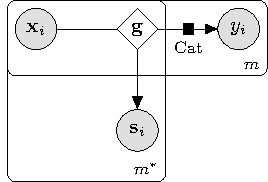
\includegraphics[width=0.35\textwidth]{results/privlearn/general_model}
\caption{Вероятностная модель в формате плоских нотаций.}
\label{fg:st:plate}
\end{figure}

На рис. \ref{fg:st:plate} показан вид вероятностной модели в графовой нотации, для произвольной функции $\mathbf{g}$. Для каждой реализации $\mathbf{g}$ соответсвующий блок требует уточнение. На рис \ref{fg:ex:synt:plate} показана более подробная реализация в случае, когда модель $\mathbf{g}$ это линейная модель.

Для задачи многоклассовой классификации рассматриваются следующие вероятностные предположения:
\begin{enumerate}
\label{st:class:1}
	\item рассматривается функция учителя $\mathbf{f}\in\mathfrak{F}_{\text{cl}}^{*}$ \eqref{eq:F:set:cl:priv};
	\item рассматривается функция ученика следующего вида $\mathbf{g}\in\mathfrak{G}_{\text{cl}}$ \eqref{eq:G:set:cl};
	\item для истинных меток рассматривается категориальное распределение $p\bigr(y|\mathbf{x}, \mathbf{g}\bigr) = \text{Cat}\bigr(\mathbf{g}\bigr(\mathbf{x}\bigr)\bigr)$, где $\mathbf{g}\bigr(\mathbf{x}\bigr)$ задает вероятность каждого класса;
	\item для меток учителя введем плотность распределения
\[
\label{reg:dist}
\begin{aligned}
	p\bigr(\mathbf{s}|\mathbf{x}, \mathbf{g}\bigr) = C\prod_{k=1}^{K}g_k\bigr(\mathbf{x}\bigr)^{s^k},
\end{aligned}
\]
где $g^k$ обозначает вероятность класса $k$, которую предсказывает модель ученика, а $s^k$ --- вероятность класса $k$, которую предсказывает модель учителя.
\end{enumerate}
\begin{theorem}
\label{theorem:st:dist}
Пусть вероятнось каждого класса отделима от нуля и единицы, то есть для всех $k$ выполняется $1 > 1- \varepsilon > g_k\bigr(\mathbf{x}\bigr) > \varepsilon > 0,$ тогда при
\[
C=\left(-1\right)^{K}\frac{K^{K/2}}{2^{K(K-1)/2}}\prod_{k=1}^{K}g_k\bigr(\mathbf{x}\bigr)\log g_k\bigr(\mathbf{x}\bigr)
\]
функция $p\bigr(\mathbf{s}|\mathbf{x}, \mathbf{g}\bigr)$ определенная в \eqref{reg:dist} является плотностью распределения.
\end{theorem}
\begin{proof}
	Во-первых покажем, что для произвольного вектора ответов $\mathbf{s} \in \mathcal{S}_K$ выполняется $p\bigr(\mathbf{s}|\mathbf{x}, \mathbf{g}\bigr) \geq 0$. Заметим, что для всех $k$ выполняется, что $\log g_k\bigr(\mathbf{x}\bigr) < 0,$ тогда
\[
\begin{aligned}
	C=\underbrace{\frac{K^{K/2}}{2^{K(K-1)/2}}}_{>0}\prod_{k=1}^{K}\underbrace{g_k\bigr(\mathbf{x}\bigr)}_{>\varepsilon}\underbrace{\left(-\log g_k\bigr(\mathbf{x}\bigr)\right)}_{>0} > 0,
\end{aligned}
\]
тогда с учетом того, что $g_k\bigr(\mathbf{x}\bigr) >0$ и $C>0$ получаем, что $p\bigr(\mathbf{s}|\mathbf{x}, \mathbf{g}\bigr) \geq 0$.
	Во-вторых покажем, что интеграл по всему пространству ответов $\mathcal{S}_K$ является конечным:
	\[
	\label{theorem:st:dist:eq:1}
	\begin{aligned}
		\int_{\mathcal{S}_K}p\bigr(\mathbf{s}|\mathbf{x}, \mathbf{g}\bigr)ds &= \int_{\mathcal{S}_K}\prod_{k=1}^{K}g_k\bigr(\mathbf{x}\bigr)^{s^k}ds = \prod_{k=1}^{K}\int_{\mathcal{S}_K}g_k\bigr(\mathbf{x}\bigr)^{s^k}ds\\ 
		& = \prod_{k=1}^{K}\int_{0}^{1}\frac{r^{K-1}\sqrt{K}}{\left(K-1\right)!\sqrt{2^{K-1}}}g_k\bigr(\mathbf{x}\bigr)^{r}dr = \prod_{k=1}^{K}\underbrace{\frac{\sqrt{K}}{\left(K-1\right)!\sqrt{2^{K-1}}}}_{D}\int_{0}^{1}r^{K-1}g_k\bigr(\mathbf{x}\bigr)^{r}dr \\
		& = D^K\prod_{k=1}^{K} \int_{0}^{1}r^{K-1}\exp\bigr(r\log g_k\bigr(\mathbf{x}\bigr)\bigr)dr \\
		& = \left(-D\right)^K\prod_{k=1}^{K}\log g_k\bigr(\mathbf{x}\bigr)\left(\Gamma\bigr(K\bigr) - \Gamma\bigr(K, -\log g_k\bigr(\mathbf{x}\bigr)\bigr)\right) \\
		& = \left(-D\right)^K\left(K-1\right)!^K\prod_{k=1}^{K}\log g_k\bigr(\mathbf{x}\bigr)\left(1 -g_k\bigr(\mathbf{x}\bigr) \exp_{K-1}\bigr(-\log g_k\bigr(\mathbf{x}\bigr)\bigr)+g_k\bigr(\mathbf{x}\bigr)\right) \\
		& = \frac{\left(-\sqrt{K}\right)^K}{2^{K(K-1)/2}}\prod_{k=1}^{K}\log g_k\bigr(\mathbf{x}\bigr)\left(1 -g_k\bigr(\mathbf{x}\bigr) \exp_{K-1}\bigr(-\log g_k\bigr(\mathbf{x}\bigr)\bigr)+g_k\bigr(\mathbf{x}\bigr)\right) < \infty,
	\end{aligned}
	\]
где $\Gamma\bigr(K\bigr)$ является гамма функцией, $\Gamma\bigr(K, -\log g_k\bigr(\mathbf{x}\bigr)\bigr)$ является неполной гамма функцией, $\exp_{n}\bigr(x\bigr)$ является суммой Тейлора из первых $n$ слагаемых. В рамках приближенных расчетов будем считать, что $\exp_{n}\bigr(x\bigr)\approx\exp\bigr(x\bigr),$ тогда с учетом \eqref{theorem:st:dist:eq:1} получаем:
	\[
	\label{theorem:st:dist:eq:2}
	\begin{aligned}
		C\bigr(\mathbf{g}, \mathbf{x}\bigr) = \int_{\mathcal{S}_K}p\bigr(\mathbf{s}|\mathbf{x}, \mathbf{g}\bigr)ds \approx \left(-1\right)^{K}\frac{K^{K/2}}{2^{K(K-1)/2}}\prod_{k=1}^{K}g_k\bigr(\mathbf{x}\bigr)\log g_k\bigr(\mathbf{x}\bigr)
	\end{aligned}
	\]
	
Полученное выражение \eqref{theorem:st:dist:eq:2} заканчивает доказательство теоремы.
\end{proof}

Из теоремы \ref{theorem:st:dist} следует, что плотность введенная для меток учителя является плотностью распределения, следовательно можно воспользоваться выражением \eqref{eq:st:12}.
Используя предположения 1)--4) и подставляя в \eqref{eq:st:12} получаем следующую оптимизационную задачу:
\[
\label{eq:st:class:1}
\begin{aligned}
\hat{\mathbf{g}} = \arg\max_{\mathbf{g}\in \mathcal{G}} & \sum_{i\not\in \mathcal{I}}\sum_{k=1}^{K}y_i^k\log g_k\bigr(\mathbf{x}_i\bigr)\bigr|_{T=1} \\
&+ \left(1-\lambda\right)\sum_{i\in \mathcal{I}}\sum_{k=1}^{K}y_i^k\log g_k\bigr(\mathbf{x}_i\bigr)\bigr|_{T=1} + \lambda\sum_{i\in \mathcal{I}}\sum_{k=1}^{K}s_{i,k}\log g_k\bigr(\mathbf{x}_i\bigr)\bigr|_{T=T_0} \\
&+ \lambda \sum_{i\in \mathcal{I}}\sum_{k=1}^{K}\left(\log g_k\bigr(\mathbf{x}_i\bigr)\bigr|_{T=T_0} + \log\log\frac{1}{g_k\bigr(\mathbf{x}_i\bigr)}\bigr|_{T=T_0}\right),
\end{aligned}
\]
где выражение $\cdot\bigr|_{T=t}$ обозначает, что в предыдущую функцию $\text{softmax}$ требуется подставить значение температуры $T$ равное некоторому значению $t$.

Проанализировав выражение \eqref{eq:st:class:1} получаем, что первые три слагаемые совпадают со слагаемыми в выражении \eqref{eq:hinton:1} при $\mathcal{I} = \{1, \cdots, m\},$ и $\lambda=\frac{1}{2}$, а третье слагаемое является некоторым регуляризатором, который получен из вида распределения.

Анализируя первые три слагаемых в выражении \eqref{eq:st:class:1} получаем, что при $T_0 = 1$ получаем сумму кросс энтропий между двумя распределениями для каждого объекта:
\begin{enumerate}
	\item первое распределение это выпуклая комбинация с весом $1-\lambda$ и $\lambda$: распределения задаваемое метками объектов $\text{Cat}\bigr(\mathbf{y}\bigr)$ и распределения задаваемого моделью учителя $\text{Cat}\bigr(\mathbf{s}\bigr)$
	\item второе распределение это распределение задаваемое плотностью распределения ответов ученика $\text{Cat}\bigr(\mathbf{g}\bigr(\mathbf{x}\bigr)\bigr)$.
\end{enumerate}
Получаем, что модель ученика восстанавливает плотность не исходных меток, а новую плотность, которая является выпуклой комбинаций плотности исходных меток и меток учителя.
Для задачи регрессии рассматриваются следующие вероятностные предположения:
\begin{enumerate}
	\item рассматривается функция учителя $\mathbf{f}\in\mathfrak{F}_{\text{rg}}^{*}$:
	\[
	\label{eq:F:set:priv}
	\begin{aligned}
	\mathfrak{F}_{\text{rg}}^* = \left\{\mathbf{f}| \mathbf{f} = \mathbf{v}^*\bigr(\mathbf{x}^*\bigr), \quad \mathbf{v}^*: \mathbb{R}^{n^*} \to \mathbb{R} \right\},
	\end{aligned}
	\]
	где $\mathbf{v}^*$ --- это дифференцируемая параметрическая функция;
	\item рассматривается функция ученика $\mathbf{g}\in\mathfrak{G}_{\text{rg}}$:
\[
\label{eq:G:set:rg}
\mathfrak{G}_{\text{rg}} = \left\{\mathbf{g}| \mathbf{g} = \mathbf{z}\bigr(\mathbf{x}\bigr), \quad \mathbf{z}: \mathbb{R}^n \to \mathbb{R}^K \right\},
\]
где $\mathbf{z}$ --- это дифференцируемая параметрическая функция;
	\item истинные метки имеют нормальное распределение
	\[
		p\bigr(y|\mathbf{x}, \mathbf{g}\bigr) = \mathcal{N}\bigr(y|\mathbf{g}\bigr(\mathbf{x}\bigr), \sigma\bigr);
	\]
	\item метки учителя распределены
	\[
		p\bigr(s| \mathbf{x}, \mathbf{g}\bigr) = \mathcal{N}\bigr(s|\mathbf{g}\bigr(\mathbf{x}\bigr), \sigma_s\bigr);
	\]
\end{enumerate}

Используя предположения 1)--4) и подставляя в \eqref{eq:st:12} получаем следующую оптимизационную задачу:
\[
\label{eq:st:reg:1}
\begin{aligned}
\hat{g} = \arg\min_{g\in \mathcal{G}} & \sum_{i\not\in \mathcal{I}}\sigma^2\left(y_i-\mathbf{g}\bigr(\mathbf{x}_i\bigr)\right)^2 \\
&+ \left(1-\lambda\right)\sum_{i\in \mathcal{I}}\sigma^2\left(y_i-\mathbf{g}\bigr(\mathbf{x}_i\bigr)\right)^2 + \lambda\sum_{i\in \mathcal{I}}\sigma_s^2\left(s_i-\mathbf{g}\bigr(\mathbf{x}_i\bigr)\right)^2.
\end{aligned}
\]
Выражение \eqref{eq:st:reg:1} записано с точностью до аддитивной константы относительно $\mathbf{g}$. 

\begin{theorem}
\label{theorem:st:reg}
Пусть множество $\mathcal{G}$ описывает класс линейных функций вида $\mathbf{g}\bigr(\mathbf{x}\bigr) = \mathbf{w}^{\mathsf{T}}\mathbf{x}.$ Тогда решение оптимизационной задачи \eqref{eq:st:reg:1} эквивалентно решению следующей задачи линейной регрессии:
\[
\label{eq:st:reg:th:st:1}
\begin{aligned}
\mathbf{y''} = \mathbf{X}\mathbf{w} + \bm{\varepsilon}, \bm{\varepsilon} \sim \mathcal{N}\bigr(\mathbf{0}, \bm{\Sigma}\bigr),
\end{aligned}
\]
где $\bm{\Sigma}^{-1}=\text{diag}\bigr(\bm{\sigma'}\bigr)$ и $\mathbf{y''}$ имеют следующий вид:
\[
\label{eq:st:reg:th:st:2}
\begin{aligned}
\sigma'_{i} &= \begin{cases}
\sigma^2, \text{если} i \not \in \mathcal{I}\\
\left(1-\lambda\right)\sigma^2+\lambda\sigma_s^2, \text{иначе}\\
\end{cases}, \\
\mathbf{y''} &= \bm{\Sigma}\mathbf{y'},\\
y'_i &= \begin{cases}
\sigma^2y_i, \text{если} i \not \in \mathcal{I}\\
\left(1-\lambda\right)\sigma^2y_i+\lambda\sigma_s^2s_i, \text{иначе}\\
\end{cases}.
\end{aligned}
\]
\end{theorem}
\begin{proof}
Обозначеним $\mathbf{a}_{\mathcal{J}} = [a_i| i \in \mathcal{J}]^{\mathsf{T}},$ где $\mathbf{a}$ произвольный вектор, а $\mathcal{J}$ произвольное не пустое индексное множество. Подвектор вектора ответов $\mathbf{y}$, для элементов которого доступна привилегированная информация обозначим $\mathbf{y}_{\mathcal{I}} = [y_i| i \in \mathcal{I}]^{\mathsf{T}}$. Аналогично обозначим матрицу $\mathbf{X}_\mathcal{I}=[\mathbf{x}_{i}| i \in \mathcal{I}]^{\mathsf{T}}$.

В случае линейной модели $\mathbf{g}\bigr(\mathbf{x}\bigr) = \mathbf{w}^{\mathsf{T}}\mathbf{x}$ выражение \eqref{eq:st:reg:1} принимает вид:
\[
\label{eq:st:reg:2}
\begin{aligned}
\hat{\mathbf{w}} = \arg\min_{\mathbf{w}\in \mathcal{W}} &  \sigma^2\left(\mathbf{y}_{\bar{\mathcal{I}}}-\mathbf{X}_{\bar{\mathcal{I}}}\mathbf{w}\right)^{\mathsf{T}}\left(\mathbf{y}_{\bar{\mathcal{I}}}-\mathbf{X}_{\bar{\mathcal{I}}}\mathbf{w}\right) \\
&+ \sigma^2\left(1-\lambda\right)\left(\mathbf{y}_{\mathcal{I}}-\mathbf{X}_{\mathcal{I}}\mathbf{w}\right)^{\mathsf{T}}\left(\mathbf{y}_{\mathcal{I}}-\mathbf{X}_{\mathcal{I}}\mathbf{w}\right) + \sigma^2_s\lambda\left(\mathbf{s}_{\mathcal{I}}-\mathbf{X}_{\mathcal{I}}\mathbf{w}\right)^{\mathsf{T}}\left(\mathbf{s}_{\mathcal{I}}-\mathbf{X}_{\mathcal{I}}\mathbf{w}\right).
\end{aligned}
\]

Раскроем скобки и сгруппируем:
\[
\label{eq:st:reg:3}
\begin{aligned}
\hat{\mathbf{w}} = \arg\min_{\mathbf{w}\in \mathcal{W}} &  \sigma^2\left(\mathbf{w}^{\mathsf{T}}\mathbf{X}^{\mathsf{T}}_{\bar{\mathcal{I}}}\mathbf{X}_{\bar{\mathcal{I}}}\mathbf{w} - 2\mathbf{y}^{\mathsf{T}}_{\bar{\mathcal{I}}}\mathbf{X}_{\bar{\mathcal{I}}}\mathbf{w}\right) \\
&+ \left(1-\lambda\right)\sigma^2\left(\mathbf{w}^{\mathsf{T}}\mathbf{X}^{\mathsf{T}}_{\mathcal{I}}\mathbf{X}_{\mathcal{I}}\mathbf{w}- 2\mathbf{y}^{\mathsf{T}}_{\mathcal{I}}\mathbf{X}_{\mathcal{I}}\mathbf{w}\right) + \lambda\sigma^2_s\left(\mathbf{w}^{\mathsf{T}}\mathbf{X}^{\mathsf{T}}_{\mathcal{I}}\mathbf{X}_{\mathcal{I}}\mathbf{w}- 2\mathbf{s}^{\mathsf{T}}_{\mathcal{I}}\mathbf{X}_{\mathcal{I}}\mathbf{w}\right)
\end{aligned}
\]
Продифференцируем выражение, приравняем к нулю и сгруппируем элементы:
\[
\label{eq:st:reg:4}
\begin{aligned}
\left(\sigma^{2}\mathbf{X}^{\mathsf{T}}_{\bar{\mathcal{I}}}\mathbf{X}_{\bar{\mathcal{I}}} + \left(1-\lambda\right)\sigma^2\mathbf{X}^{\mathsf{T}}_{\mathcal{I}}\mathbf{X}_{\mathcal{I}} + \lambda\sigma^{2}_s\mathbf{X}^{\mathsf{T}}_{\mathcal{I}}\mathbf{X}_{\mathcal{I}}\right) \mathbf{w} =& 2\sigma^2\mathbf{X}^{\mathsf{T}}_{\bar{\mathcal{I}}}\mathbf{y}_{\bar{\mathcal{I}}} \\
&+ 2\left(1-\lambda\right)\sigma^2\mathbf{X}^{\mathsf{T}}_{\mathcal{I}}\mathbf{y}_{\mathcal{I}} + 2\lambda\sigma_s^2\mathbf{X}^{\mathsf{T}}_{\mathcal{I}}\mathbf{s}_{\mathcal{I}}.
\end{aligned}
\]
Воспользуемся следующими равенствами:
\[
\label{eq:st:reg:simp}
\begin{aligned}
\sigma^{2}\mathbf{X}^{\mathsf{T}}_{\bar{\mathcal{I}}}\mathbf{X}_{\bar{\mathcal{I}}} + \left(1-\lambda\right)\sigma^2\mathbf{X}^{\mathsf{T}}_{\mathcal{I}}\mathbf{X}_{\mathcal{I}} + \lambda\sigma^{2}_s\mathbf{X}^{\mathsf{T}}_{\mathcal{I}}\mathbf{X}_{\mathcal{I}} &= \mathbf{X}^{\mathsf{T}}\bm{\Sigma}^{-1}\mathbf{X},\\
2\sigma^2\mathbf{X}^{\mathsf{T}}_{\bar{\mathcal{I}}}\mathbf{y}_{\bar{\mathcal{I}}} + 2\left(1-\lambda\right)\sigma^2\mathbf{X}^{\mathsf{T}}_{\mathcal{I}}\mathbf{y}_{\mathcal{I}} + 2\lambda\sigma_s^2\mathbf{X}^{\mathsf{T}}_{\mathcal{I}}\mathbf{s}_{\mathcal{I}} &= 2\mathbf{X}\mathbf{y'},
\end{aligned}
\]
где $\bm{\Sigma}$ и $\mathbf{y'}$ из условия задачи \eqref{eq:st:reg:th:st:2}.

Подставляя \eqref{eq:st:reg:simp} в \eqref{eq:st:reg:4} получаем:
\[
\label{eq:st:reg:5}
\begin{aligned}
\mathbf{w} = 2\left(\mathbf{X}^{\mathsf{T}}\bm{\Sigma}^{-1}\mathbf{X}\right)^{-1}\mathbf{X}\bm{\Sigma}^{-1}\mathbf{y''},
\end{aligned}
\]
что соответсвует решению задачи \eqref{eq:st:reg:th:st:1}.
\end{proof}

Теорема \ref{theorem:st:reg} показывает, что обучения с учителем для задачи регрессии можно свести к классической задачи оптимизации для задачи линейной регрессии.

\subsection{Анализ вероятностного подхода к дистилляции моделей линейных моделей}
Проводится вычислительный эксперимент для анализа качества моделей, которые получены путем дистилляции модели учителя в модель ученика. Как показано в теореме \ref{theorem:st:reg} задачу регрессии с учителем можно свести к задачи регрессии без учителя, поэтому в эксперименте более подробно рассматривается случай классификации. Во всех частях вычислительного эксперимента для поиска оптимальных параметров нейросетей использовался градиентный метод оптимизации Адам \cite{kingma2014}.

В данной части проводится эксперимент для задачи классификации для выборки FashionMNIST \cite{fashionmnist}. В качестве модели учителя $\mathbf{f}$ рассматривается модель нейросети с двумя сверточными слоями и с тремя полносвязными слоями, в качестве функции активации рассматривается ReLu. Модель учителя содержит $ 30$ тысяч обучаемых параметров. В качестве модели ученика рассматривается модель логистической регрессии для многоклассовой классификации. Модель ученика содержит $7850$ обучаемых параметров.

\begin{figure}[h!t]\center
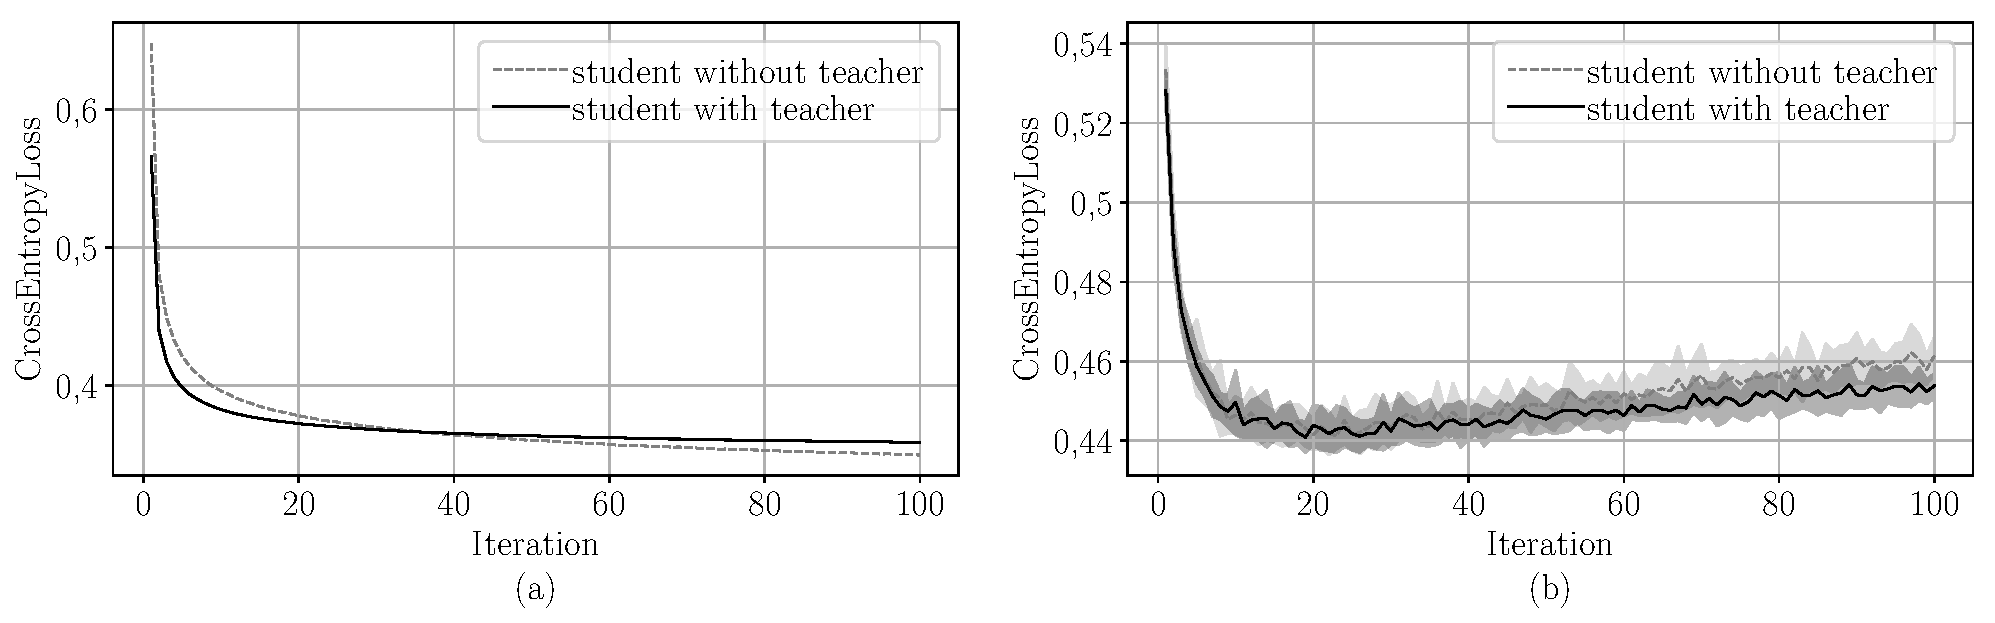
\includegraphics[width=1\textwidth]{results/privlearn/mnist_loss}
\caption{Зависимость кросс--этропии между истинными метками и предсказанными учеников вероятностями классов: a) на обучающей выборке; b) на тестовой выборке.}
\label{fg:ex:fashionmnist:loss}
\end{figure}

На рис. \ref{fg:ex:fashionmnist:loss} показан график зависимости кросс--энтропии между истинными метками объектов и вероятностями, которые предсказывает модель ученика. На графике сравнивается моделя, которая обучалась без учителя (в задаче оптимизации \eqref{eq:st:class:1} присутствует только первое слагаемое) с моделью, которая была получена путем дистилляции модели нейросети в линейную модель. На графике видно, что обе модели начинают переобучатся после 30-й итерации, но модель, которая получена путем дистилляции переобувается не так быстро, что следует из того, что ошибка на тестовой выборке растет медленней, а на обучающей выборке падает также медленней.


Проанализируем модель на синтетической выборке. Выборка построенная следующим образом:
\[
\begin{aligned}
\mathbf{W} &= \left[\mathcal{N}\bigr(w_{jk}|0, 1\bigr)\right]_{n\times K}, \quad &\mathbf{X} &= \left[\mathcal{N}\bigr(x_{ij}|0, 1\bigr)\right]_{m\times n}, \\
 \mathbf{S} &= \text{softmax}\left(\mathbf{XW}\right), \quad &\mathbf{y} &= \left[\text{Cat}\bigr(y_i| \mathbf{s}_i\bigr)\right],
\end{aligned}
\]
где функция $\text{softmax}$ берется построчно. Строки матрицы $\mathbf{S}$ будем рассматривать как предсказание учителя, то есть учитель знает истинные вероятности каждого класса. На рис. \ref{fg:ex:synt:plate} показана вероятностная модель в графовой нотации. В эксперименте число признаков $n=10$, число классов $K=3$, для обучения было сгенерировано $m_{\text{train}}=1000$ и $m_{\text{test}}=100$ объектов.

На рис. \ref{fg:ex:synt:distr:real} показано распределение по классам для каждого объекта обучающей выборки. Видно, что все классы являются равновероятными.

Построим в качестве ученика простую линейную модель, которая минимизирует крос--энтропийную (первое слагаемое в формуле \eqref{eq:st:class:1}). Представление данной модели в виде графовой модели показано на рис. \ref{fg:ex:synt:plate}.

\begin{figure}[h!t]\center
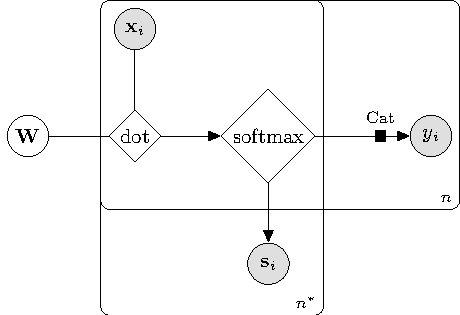
\includegraphics[width=0.35\textwidth]{results/privlearn/linear_model}
\caption{Вероятностная модель используемая в синтетическом эксперименте.}
\label{fg:ex:synt:plate}
\end{figure}

\begin{figure}[h!t]\center
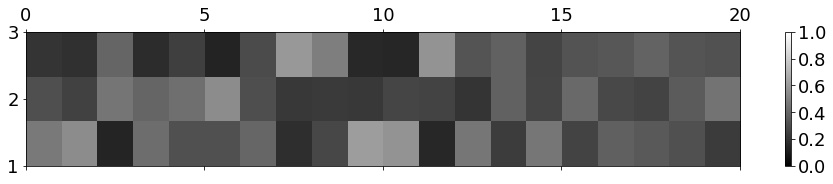
\includegraphics[width=1\textwidth]{results/privlearn/syn_real_distr}
\caption{Истинное распределение  объектов по классам.}
\label{fg:ex:synt:distr:real}
\end{figure}


На рис. \ref{fg:ex:synt:distr:without} показано распределение вероятностей классов, которое предсказала модель. Видно, что данное распределение является не соответствует истинному, так как модель сосредотачивает всю вероятность в одном классе.

\begin{figure}[h!t]\center
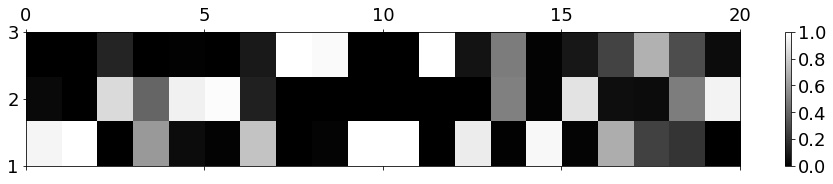
\includegraphics[width=1\textwidth]{results/privlearn/syn_without_teacher_distr}
\caption{Распределение предсказанное моделью без использования информации об истинном распределение на классах.}
\label{fg:ex:synt:distr:without}
\end{figure}

\begin{figure}[h!t]\center
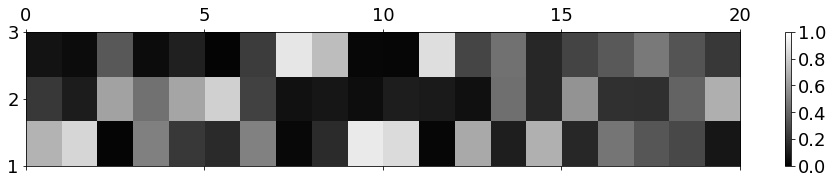
\includegraphics[width=1\textwidth]{results/privlearn/syn_with_teacher_distr}
\caption{Распределение предсказанное моделью c использования информации об истинном распределение на классах.}
\label{fg:ex:synt:distr:with}
\end{figure}

\begin{figure}[h!t]\center
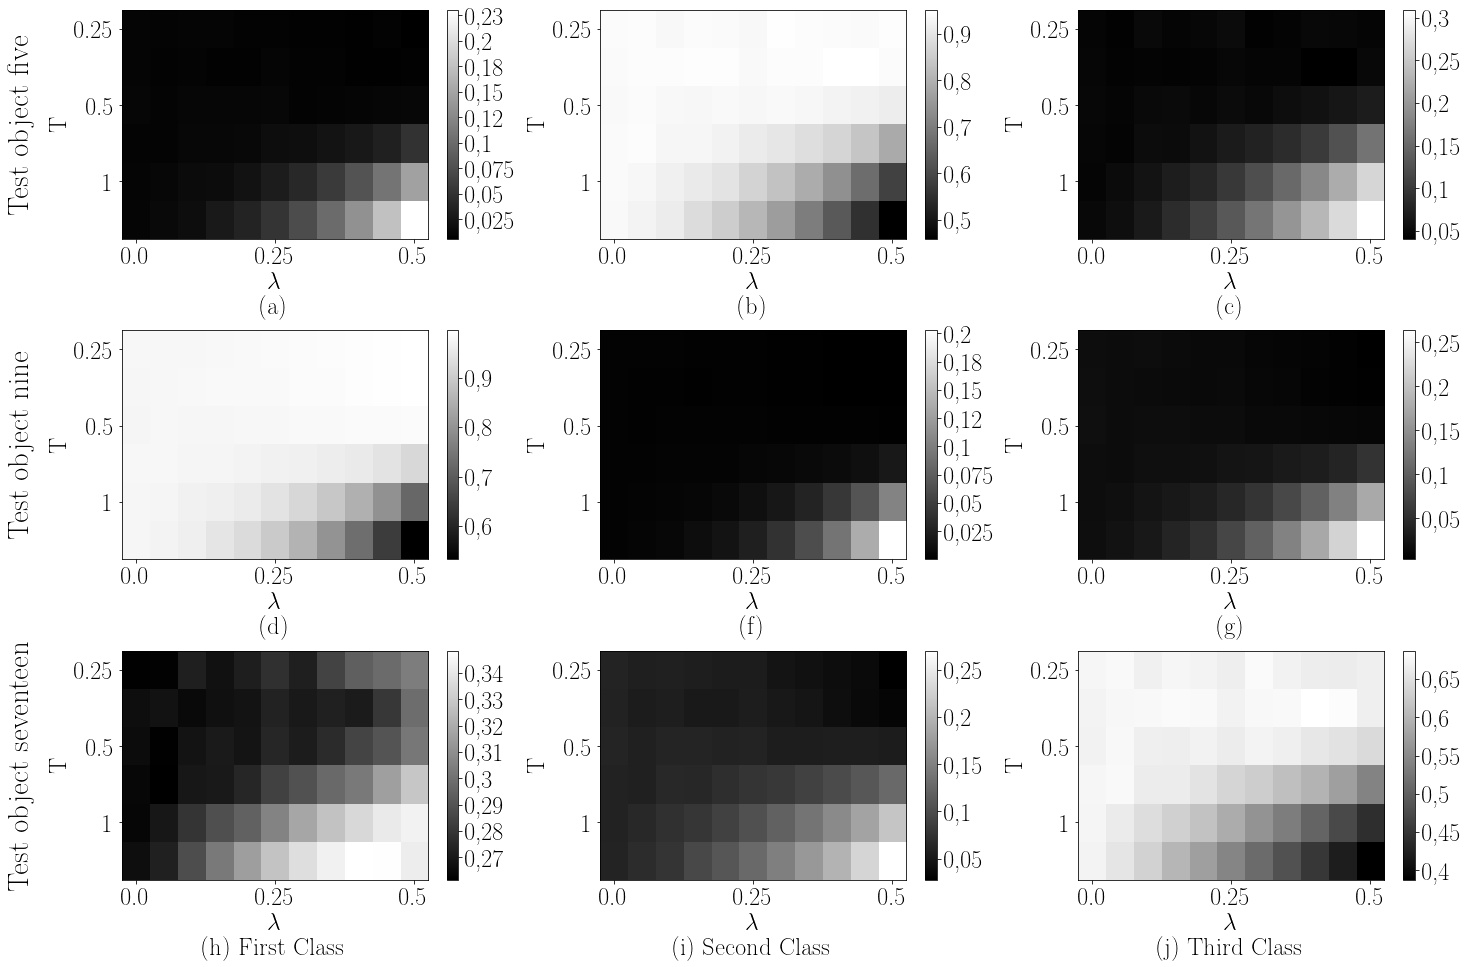
\includegraphics[width=1\textwidth]{results/privlearn/syn_T_lambda}
\caption{Вероятности классов для разных объектов.}
\label{fg:ex:synt:distr:lambda_T}
\end{figure}

Рассмотрим модель, которая учитывает информацию о истинных распределениях на классах для каждого объекта. Для этого будем минимизировать первые три слагаемых в формуле \eqref{eq:st:class:1}, при $T_0=1$ и $\lambda=0{,}75$. В качестве меток учителя $s_{i,k}$ использовались истинные вероятности для каждого класса для данного объекта. На рис \ref{fg:ex:synt:distr:with} показано распределение, которое дала модель в данном случае, видно, что распределения являются сглаженными и концентрации всей вероятности в одном классе не наблюдается.

Заметим, что в данном примере предполагается, что модель учителя учитывает не только метки классов, а и распределение на метках классов, в то время как в выборке $\mathcal{D} = \{\mathbf{X}, \mathbf{y}\},$ имеются только точечные оценки в виде меткок. 

В данном примере используются истинные распределения в качестве предсказаний учителя, но их можно заменить предсказаниями модели учителя, которая предсказывает не только сами меток, а и их распределение для каждого объекта.

На рис. \ref{fg:ex:synt:distr:lambda_T} показана зависимость вероятности верного класса от температуры $T$ и параметра доверия $\lambda$ для одного из объекта из тестовой выборке. Видно, что при увеличении темпертуры распределение на классас становится более равномерным.

В данной части проводится эксперимент на выборке Twitter Sentiment Analysis. Данная выборка содержит короткие сообщения, для которых нужно предсказать эмоциональный окрас: содержит твит позитивный окрас или негативный. Выборка разделена на $1{,}18$ миллиона твитов для обучения и $0{,}35$ миллиона твитов для тестирования. В твитах была выполнена следующая предобработка:
\begin{itemize}
	\item все твиты были переведены в нижний регистр;
	\item все никнеймы вида ``@andrey'' были заменены на токен ``name'';
	\item все цифры были заменены на токен ``number''.
\end{itemize}
Результаты данной части эксперимента показаны в табл. \ref{tb:ce:1}. В качестве модели учителя использовалась модель Bi-LSTM с $170$ тысячами параметров для обучения. В качестве эмбедингов обучалась матрица из $30$ миллионов параметров в единой процедуре с моделью BI-LSTM. Обученная модель предсказывает с точностью $0{,}835$. В качестве модели ученика рассматривается модель с $1538$ параметрами, но в качестве эмбедингов рассматривается переобученная модель BERT.

\begin{table}[]
\caption{Сводная таблица результатов вычислительного эксперимента.}
\label{tb:ce:1}
\begin{center}
\begin{tabular}{|l|l|c|c|c|}
\hline
\multicolumn{1}{|c|}{Dataset} & \multicolumn{1}{c|}{Model} & CrossEntropyLoss      & Accuracy    &   StudentSize   \\ \hline
\multirow{2}{*}{FashionMnist} & without teacher    &  $0{,}461 \pm 0{,}005$ & $0{,}841\pm 0{,}002$ & 7850 \\ \cline{2-5} 
                              & with teacher       & $0{,}453 \pm 0{,}003$ & $0{,}842 \pm 0{,}002$ & 7850\\ \hline
\multirow{2}{*}{Synthetic}    & without teacher    & $0{,}225 \pm 0{,}002$ & $0{,}831\pm 0{,}002$ & 33 \\ \cline{2-5} 
                              &  with teacher       & $0{,}452 \pm 0{,}001$   & $0{,}828\pm 0{,}001$ & 33 \\ \hline
\multirow{2}{*}{Twitter }    & without teacher    & $0{,}501 \pm 0{,}006$ & $0{,}747\pm 0{,}005$ & $1538$  \\ \cline{2-5} 
                              &with teacher       & $0{,}489 \pm 0{,}003$   & $0{,}764\pm 0{,}004$ & $1538$ \\ \hline
\end{tabular}
\end{center}
\end{table}

\newpage


\section{Байесовская дистилляция моделей глыбокого обучения}
\subsection{Описание задачи}
Исследуется проблема снижения числа обучаемых параметров моделей машинного обучения. Примерами таких моделей, с избыточным число параметров, являются AlexNet~\cite{Krizhevsky2012}, VGGNet~\cite{Simonyan2014}, ResNet~\cite{Kaiming2015}, BERT~\cite{Devlin2018, Vaswani2017}, mT5~\cite{Linting2021}, GPT3\cite{Brown2020} и другие.
\begin{table}[h!]
\caption{Число параметров в моделях машинного обучения.}
\label{tb:intro:1}
\begin{center}
\resizebox{\textwidth}{!}{
\begin{tabular}{|l|l|l|l|l|l|l|}
\hline
Название               & AlexNet     & VGGNet      & ResNet      & BERT     & mT5   & GPT3  \\ \hline
Год                          & 2012        & 2014        & 2015        & 2018     & 2020  & 2020  \\ \hline
Тип данных             & изображение & изображение & изображение & текст    & текст & текст \\ \hline
Число параметров, млрд & $0{,}06$    & $0{,}13$    & $0{,}06$    & $0{,}34$ & $13$  & $175$ \\ \hline
\end{tabular}
}
\end{center}
\end{table}
Табл.~\ref{tb:intro:1} описывает глубокие модели машинного обучения.
Число параметров моделей машинного обучения с годами растет.
Это влечет снижение интерпретируемости моделей.
Данная проблема рассматривается в специальном классе задач по состязательным атакам (англ. adversarial attack)~\cite{Zheng2020}.
Большое число параметров требует больших вычислительных ресурсов.
Из-за этого данные модели не могут быть использованы в мобильных устройствах.
Для снижения числа параметров предложен метод дистилляции модели~\cite{Hinton2015, Vapnik2015, Lopez2016}.
Дистиллируемая модель с большим числом параметров называется~\textit{учитель}, а модель получаемая путем дистилляции называется~\textit{ученик}.
При оптимизации параметров модели ученика используется модель учителя с фиксированными параметрами.
\begin{definition}
Дистилляция модели~--- снижение сложности модели путем выбора модели в множестве более простых моделей на основе параметров и ответов более сложной фиксированной модели.
\end{definition}

Идея дистилляции предложена в работах Дж.\,Е. Хинтона и В.\,Н. Вапником~\cite{Hinton2015, Vapnik2015, Lopez2016}. В этих работах предлагается использовать ответы учителя в качестве целевой переменной для обучения модели ученика.
Поставлен ряд экспериментов, в которых проводилась дистилляция моделей для задачи классификации машинного обучения.
Базовый эксперимент на выборке MNIST~\cite{mnist} показал применимость метода для дистилляции избыточно сложной нейросетевой модели в нейросетевую модель меньшей сложности.
Эксперимент по дистилляции ансамбля моделей в одну модель для решения задачи распознания речи. Также в работе~\cite{Hinton2015} был проведен эксперимент по обучению экспертных моделей на основе одной модели с большим числом параметров при помощи предложенного метода дистилляции на ответах учителя.

В работе~\cite{Zehao2017} предложен метод передачи селективности нейронов (англ. neuron selectivity transfer) основаный на минимизации специальной функции потерь основаной на максимальном среднем отклонении (англ. maximum mean discrepancy) между выходами всех слоев модели учителя и ученика. Вычислительный эксперимент показал эффективность данного метода для задачи классификации изображений на примере выборок CIFAR~\cite{cifar10} и ImageNet~\cite{imagenet}.

В данной работе предлагается метод,ы основанный на байесовском выводе.
В качестве априорного распределения параметров модели ученика предлагается использовать апостериорное распределение параметров модели учителя.
Решается задача сопоставления пространства параметров модели учителя и модели ученика.
Авторы предлагают подход, основаный на последовательном сопоставлении пространств параметров модели ученика и учителя. 
\begin{definition}
\label{def:structure}
Структура модели~--- множество структурных параметров модели, которые задают вид суперпозиции.
\end{definition}
\begin{definition}
\label{def:sopos}
Сопоставление параметрических моделей~--- изменение структуры модели (одной или нескольких моделей) в результате которого векторы параметров различных моделей лежат в одном пространстве.
\end{definition}
В результате сопоставления, параметры модели учителя и модели ученика лежат в одном пространстве.
Как следствие, в качестве априорного распределения параметров модели ученика выбирается апостериорное распределение параметров модели учителя.
В данной работе в качестве параметрических моделей рассматривается полносвязная нейронная сеть.
В качестве структурных параметров модели выбраны число слоев, а также размер каждого скрытого слоя.

В рамках предложенного метода сопоставления параметрических моделей не оговорен выбор порядка на множестве параметров модели учителя.
Для этого предлагается упорядочивать параметры модели учителя на основе их значимости.
Первый нейрон является наиболее значимым, а последний нейрон наименее значимым.
Порядок задается на основе отношения плотности распределения упорядочивваемого параметра к плотности распределения параметра в нуле~\cite{graves2011} или на основе метода Белсли~\cite{grabovoy2019}.
В рамках данной работы порядок на параметрах в рамках одного слоя задается случайный образом.

В рамках вычислительного эксперимента проводится теоретический анализ. Предложенный метод дистилляции анализируется на примере синтетической выборки, а также на реальной выборке FashionMnist~\cite{fashionmnist}.

\subsection{Постановка задачи дистилляции}
Задана выборка
\begin{gather}
\label{eq:st:1}
\begin{aligned}
\mathfrak{D} = \left\{\left(\mathbf{x}_i, y_i\right)\right\}_{i=1}^{m}, \qquad \mathbf{x}_i \in \mathbb{R}^{n}, \quad y_i \in \mathbb{Y},
\end{aligned}
\end{gather}
где~$\mathbf{x}_i, y_i$~--- признаковое описание и целевая переменная~$i$-го объекта, число объектов в обучающей выборке обозначается~$m$. Размер признакового описания объектов обозначается~$n$. Множество~$\mathbb{Y}=\{1,\cdots,K\}$ для задачи классификации, где~$K$ число классов, множество $\mathbb{Y}=\mathbb{R}$ для задачи регрессии.

Задана модель учителя в виде суперпозиций линейных и нелинейных преобразований:
\begin{gather}
\label{eq:st:2}
\begin{aligned}
f = \bm{\sigma} \circ \mathbf{U}_T \bm{\sigma} \circ \mathbf{U}_{T-1}\circ \cdots  \mathbf{U}_2\bm{\sigma} \circ \mathbf{U}_1,
\end{aligned}
\end{gather}
где~$T$~--- число слоев модели учителя, $\bm{\sigma}$~--- функция активации, а $\mathbf{U}_t$ обозначает матрицу линейного преобразования. Матрицы~$\mathbf{U}$ соединяются в вектор параметров~$\mathbf{u}$ модели учителя~$f$:
\begin{gather}
\label{eq:st:2.1}
\begin{aligned}
\mathbf{u} = \text{vec}\bigr(\left[\mathbf{U}_T, \mathbf{U}_{T-1}, \cdots \mathbf{U}_1\right]\bigr),
\end{aligned}
\end{gather}
где~$\text{vec}$ операция векторизации соединенных матриц.
Каждая матрица~$\mathbf{U}_t$ имеет размер~$n_t\times n_{t-1},$ где $n_0=n,$ а  $n_T={1}$ для задачи регрессии и $n_T=K$ для задачи классификации на $K$ классов. Число параметров~$N_{\text{tr}}$ учителя~$f$
\begin{gather}
\label{eq:st:2.2}
\begin{aligned}
N_{\text{tr}} = \sum_{t=1}^{T}n_tn_{t-1}.
\end{aligned}
\end{gather}
Для построения вектора параметров~$\mathbf{u}$ задается полный порядок на элементов матриц~$\mathbf{U}_t$. Для полносвязнной нейронной сети вводится естественный порядок, индуцированный номером слоя~$t$, номером нейрона, и номером элемента вектора параметров нейрона: выбирается матрица~$\mathbf{U}_t$, строка этой матрицы и элемент строки.

Например, для модели учителя в задаче регрессии:
\begin{gather}
\label{eq:st:3}
\begin{aligned}
f\bigr(\mathbf{x}\bigr) = \bm{\sigma} \circ \mathbf{U}_3 \bm{\sigma} \circ \mathbf{U}_2\bm{\sigma}\circ \mathbf{U}_1\mathbf{x},
\end{aligned}
\end{gather}
вектор параметров~$\mathbf{u}$ принимает ви
\begin{gather}
\label{eq:st:4}
\begin{aligned}
\mathbf{u} = \bigr[u_1^{1,1}, \cdots, u_1^{1,n},
                                               \cdots, 
                             u_1^{n_1,1}, \cdots, u_1^{n_1,n},  
                             u_2^{1, 1}, \cdots, u_2^{1, n_1}, 
                                                \cdots, 
                            u_2^{n_2, 1}, \cdots, u_2^{n_2, n_1},
                            u_3^{1, 1}, \cdots, u_3^{1, n_2}\bigr].
\end{aligned}
\end{gather}
Пусть для вектора параметров учителя~$f$ известно апостериорное распределение параметров~$p\bigr(\mathbf{u}|\mathfrak{D}\bigr)$. 
На основе выборки~$\mathfrak{D}$ и апостериорного распределения параметров учителя~$f$ требуется выбрать модель ученика из параметрического семейства функций:
\begin{gather}
\label{eq:st:5}
\begin{aligned}
g = \bm{\sigma} \circ \mathbf{W}_L\bm{\sigma}  \circ \cdots \circ \mathbf{W}_1, \quad \mathbf{W}_l \in \mathbb{R}^{n_l \times n_{l-1}},
\end{aligned}
\end{gather}
где~$L$ число слоев модели ученика.
Число параметров~$N_{\text{st}}$ модели ученика~$g$ вычисляется аналогично выражению~\eqref{eq:st:2.2}.
Вектор параметров модели ученика~$\mathbf{w}$ строится аналогичным образом~\eqref{eq:st:2.1}.
Модель~$g$ задается своим вектором параметров~$\mathbf{w}$.
Следовательно, задача выбора модели~$g$ эквивалентна задаче оптимизации вектора параметров~$\mathbf{w}\in\mathbb{R}^{N_{\text{st}}}$.

Параметры~$\hat{\mathbf{w}} \in \mathbb{R}^{N_{\text{st}}}$ оптимизируются при помощи вариационного вывода на основе совместного правдоподобия модели и данных:
\begin{gather}
\label{eq:st:6}
\begin{aligned}
\mathcal{L}\bigr(\mathfrak{D}, \mathbf{A}\bigr) = \log p\bigr(\mathfrak{D}|\mathbf{A}\bigr) = \log \int_{\mathbf{w} \in \mathbb{R}^{N_{\text{st}}}}p\bigr(\mathfrak{D}|\mathbf{w}\bigr)p\bigr(\mathbf{w}|\mathbf{A}\bigr)d\mathbf{w},
\end{aligned}
\end{gather}
где~$p\bigr(\mathbf{w}| \mathbf{A}\bigr)$~--- априорное распределение вектора параметров модели ученика.
Так как взятие интеграла~\eqref{eq:st:6} является вычислительно сложной задачей, используется вариационный подход~\cite{graves2011, grabovoy2019}. Для этого задается вариационное распределение параметров модели ученика~$q\bigr(\mathbf{w}|\bm{\mu}, \bm{\Sigma}\bigr),$ которое аппроксимирует неизвестное апостериорное распределение~$p\bigr(\mathbf{w}|\mathfrak{D}\bigr)$
\begin{gather}
\label{eq:st:new:1}
\begin{aligned}
q\bigr(\mathbf{w}|\bm{\mu}, \bm{\Sigma}\bigr) \approx  p\bigr(\mathbf{w}|\mathfrak{D}\bigr).
\end{aligned}
\end{gather}
Далее распределение $q\bigr(\mathbf{w}|\bm{\mu}, \bm{\Sigma}\bigr)$ обозначается просто~$q\bigr(\mathbf{w}\bigr).$ Оптимизация параметров~$\mathbf{w}$ сводится к решению  задачи:
\begin{gather}
\label{eq:st:7}
\begin{aligned}
\hat{\mathbf{w}} = \arg \min_{\bm{\mu}, \bm{\Sigma}, \mathbf{w}} \text{D}_{\text{KL}}\bigr(q\bigr(\mathbf{w}|\bm{\mu}, \bm{\Sigma}\bigr)||p\bigr(\mathbf{w}|\mathbf{A}\bigr)\bigr) - \log p\bigr(\mathbf{y}|\mathbf{X}, \mathbf{w}\bigr).
\end{aligned}
\end{gather}
Выражение~\eqref{eq:st:7} не учитывает параметры учителя~$f$. Для использования информации о распределении параметов учителя предлагается рассмотреть параметры априорного распределения~$p\bigr(\mathbf{w}|\mathbf{A}\bigr)$ как функцию от апостериорного распределения учителя~$p\bigr(\mathbf{u}|\mathfrak{D}\bigr)$.

\subsection{Построение априорного распределения ученика}
Апостериорное распределение параметров модели учителя предполагается нормальным:
\begin{gather}
\label{eq:ap:1}
\begin{aligned}
p\bigr(\mathbf{u}|\mathfrak{D}\bigr) = \mathcal{N}\bigr(\mathbf{m}, \bm{\Sigma}\bigr),
\end{aligned}
\end{gather}
где~$\mathbf{m}$ и~$\bm{\Sigma}$ параметры этого распределения. На основе параметров~$\mathbf{m}$ и~$\bm{\Sigma}$ требуется задать параметры~$\mathbf{A}$ априорного распределения~$p\bigr(\mathbf{w}|\mathbf{A}\bigr).$
В случае, когда структура моделей учителя и ученика задаются числом слоев и размером этих слоев, то возможны следующие варианты: 1) число слоев и размер каждого слоя совпадает; 2) число слоев совпадает, а размеры различаются; 3) не совпадает число слоев.

\paragraph{Учитель и ученик принадлежат одному семейству.}
\label{section:one:space}
Рассмотрим следующие условия:
\begin{enumerate}
    \item число слоев модели учителя равняется числу слоев модели ученика $L=T$;
    \item размеры соответствующих слоев совпадают, другими словами, для всех $t, l$ таких, что $t=l$ выполняется $n_l = n_t,$ где $n_t$ обозначает размер $t$-го слоя учителя, а $n_l$ размер $l$-го слоя ученика.
\end{enumerate}
В случае выполнения этих условий, априорное распределение параметров модели ученика приравнивается к апостериорному распределения параметров учителя $p\bigr(\mathbf{w}|\mathbf{A}\bigr) = p\bigr(\mathbf{u}|\mathfrak{D}\bigr)$.

\paragraph{Удаление нейрона в слое учителя.}
Проведем согласование модели учителя и модели ученика, согласно определению~\ref{def:sopos} при помощи последовательных преобразований параметров~$\mathbf{u}$. Рассмотрим преобразование:
\begin{gather}
\label{eq:ap:2}
\begin{aligned}
\phi\bigr(t, \mathbf{u}\bigr) : \mathbb{R}^{N_{\text{tr}}} \to \mathbb{R}^{N_{\text{tr}}-2n_t}
\end{aligned}
\end{gather}
вектора~$\mathbf{u},$ которое описывает удаление одного нейрона из~$t$-го слоя учителя.
%Другими словами, преобразование~$\phi\bigr(t\bigr)$ зануляет одну из строк матрицы~$\mathbf{U}_t$. Заметим, что данное зануление влечет зануление соответствующего столбца матрицы~$\mathbf{U}_{t+1}$.
Обозначим новый вектор параметров~$\bm{\upsilon} =  \phi\bigr(t, \mathbf{u}\bigr),$ а элементы вектора, которые были удалены как~$\bar{\bm{\upsilon}}.$ Заметим, что векторы~$\bm{\upsilon}$ и $\bar{\bm{\upsilon}}$ являются случайными величинами. 
%Введем следующие обозначения:
%\begin{gather}
%\label{eq:ap:def:1}
%\begin{aligned}
%\bm{\upsilon} _{0} = \mathsf{E}\bm{\upsilon} , \quad \bar{\bm{\upsilon}}_0 = \mathsf{E}\bar{\bm{\upsilon}}, \quad  \bm{\Sigma}_{\bm{\upsilon},\bm{\upsilon}} = \text{cov}\bigr(\bm{\upsilon},\bm{\upsilon}\bigr), \quad  \bm{\Sigma}_{\bm{\upsilon},\bar{\bm{\upsilon}}} = \text{cov}\bigr(\bm{\upsilon},\bar{\bm{\upsilon}}\bigr), \quad  \bm{\Sigma}_{\bar{\bm{\upsilon}},\bar{\bm{\upsilon}}} = \text{cov}\bigr(\bar{\bm{\upsilon}},\bar{\bm{\upsilon}}\bigr),\\
%\end{aligned}
%\end{gather}
%где~$ \text{cov}\bigr(\bm{\upsilon},\bm{\upsilon}\bigr)$ обозначает ковариационную матрицу.
\begin{theorem}
\label{theorem:ap:neural}
Пусть выполняются следующие условия:
\begin{enumerate}
\item апостериорное распределение~$p\bigr(\mathbf{u}|\mathfrak{D}\bigr)$ параметров модели учителя является нормальным распределением~\eqref{eq:ap:1};
\item число слоев модели учителя равняется числу слоев модели ученика $L=T$;
\item размеры соответствующих слоев не совпадают, другими словами, для всех $t, l$ таких, что $t=l$ выполняется $n_t \leq n_l,$.
\end{enumerate}
Тогда апостериорное распределения параметров модели учителя~$p\bigr(\bm{\upsilon}|\mathfrak{D}\bigr)$ также является нормальным распределением.
%\begin{gather}
%\label{eq:ap:3}
%\begin{aligned}
%p\bigr(\bm{\upsilon}|\mathfrak{D}\bigr) = \mathcal{N}\bigr(\bm{\upsilon}_{0}+\bm{\Sigma}_{\bm{\upsilon},\bar{\bm{\upsilon}}}\bm{\Sigma}_{\bar{\bm{\upsilon}},\bar{\bm{\upsilon}}}^{-1}\left(\mathbf{0} - \bar{\bm{\upsilon}}\right), \bm{\Sigma}_{\bm{\upsilon},\bar{\bm{\upsilon}}}\bm{\Sigma}_{\bar{\bm{\upsilon}},\bar{\bm{\upsilon}}}^{-1}\bm{\Sigma}_{\bm{\upsilon},\bar{\bm{\upsilon}}}\bigr).
%\end{aligned}
%\end{gather}
\end{theorem}
\begin{proof}
Не уменьшая общности, пусть~$\phi\bigr(t, \mathbf{u}\bigr)$ удаляет $j$-й нейрон в $t$-м слое, что является удалением $j$-й строки матрицы $\mathbf{U}_t$. Заметим, что удаление $j$-й строки матрицы $\mathbf{U}_t$ влечет удаление $j$-й компоненты вектора $z_{t+1}$, где
\begin{gather}
\label{eq:ap:tr:neural:1}
\begin{aligned}
\mathbf{z}_{t} = \bm{\sigma} \circ \mathbf{U}_{t-1} \bm{\sigma} \circ \cdots  \mathbf{U}_2\bm{\sigma} \circ \mathbf{U}_1\mathbf{x}.
\end{aligned}
\end{gather}

Удаление $j$-й компоненты вектора $\mathbf{z}_{t+1}$ эквивалентно занулению~$j$-го столбца матрицы~$\mathbf{U}_{t+1}.$ Заметим, что тогда предсказание модели не зависит от параметров~$j$-й строки матрицы~$\mathbf{U}_t,$ а следовательно донными параметрами также можно пренебречь.

Найдем распределение вектора~$\bm{\upsilon}.$ Для поиска распределения вектора параметров после зануления~$j$-го столбца матрицы~$\mathbf{U}_{t+1}$ воспользуемся формулой условной вероятности~$p\bigr(\bar{\bm{\nu}}_1|\mathfrak{D}, \bm{\nu}_1=\mathbf{0}\bigr)$, а для удаления~$j$-й строки матрицы~$\mathbf{U}_{t}$ воспользуемся маргинализацией распределения~$p\bigr(\bar{\bm{\nu}}_1|\mathfrak{D}, \bm{\nu}_1=\mathbf{0}\bigr)$. Обозначим зануляемые параметры модели как~$\bm{\nu}_1,$ а удаляемые параметры как~$\bm{\nu}_2.$ Также обозначим все параметры, которые не были занулены как~$\bar{\bm{\nu}}_1 = [\bm{\upsilon}^{\mathsf{T}}, \bm{\nu}_2^{\mathsf{T}}].$ Итоговое распределение параметров принимает  вид:
\begin{gather}
\label{eq:ap:tr:1:1}
\begin{aligned}
p\bigr(\bm{\upsilon}|\mathfrak{D}\bigr)  = \int_{\bm{\nu}_2}p\bigr(\bar{\bm{\nu}}_1|\mathfrak{D}, \bm{\nu}_1=\mathbf{0}\bigr) d\bm{\nu}_2.
\end{aligned}
\end{gather}

Из свойств нормального распределения следует, что распределение
\begin{gather}
\label{eq:ap:tr:neural:2}
\begin{aligned}
p\bigr(\bar{\bm{\nu}}_1|\mathfrak{D}, \bm{\nu}_1=\mathbf{0}\bigr)
\end{aligned}
\end{gather}
также является нормальным распределением с параметрами $\bm{\mu}, \bm{\Xi}$:
\begin{gather}
\label{eq:ap:tr:1:1}
\begin{aligned}
\bm{\mu} &= \mathbf{m}_{\bar{\bm{\nu}}_1}+\bm{\Sigma}_{\bar{\bm{\nu}}_1,\bm{\nu}_1} \bm{\Sigma}_{\bm{\nu}_1,\bm{\nu}_1}^{-1} \left(\mathbf{0} - \mathbf{m}_{\bm{\nu}_1}\right), \\
 \bm{\Xi} &= \bm{\Sigma}_{\bar{\bm{\nu}}_1,\bar{\bm{\nu}}_1} - \bm{\Sigma}_{\bar{\bm{\nu}}_1,\bm{\nu}_1} \bm{\Sigma}_{\bm{\nu}_1,\bm{\nu}_1}^{-1} \bm{\Sigma}_{\bar{\bm{\nu}}_1,\bm{\nu}_1},
\end{aligned}
\end{gather}
где введены обозначения~$\mathbf{m}_{\bar{\bm{\nu}}_1}, \mathbf{m}_{\bm{\nu}_1}$ соответствует подвектору вектора~$\mathbf{m},$ который относится к параметрам~$\bar{\bm{\nu}}_1$ и $\bm{\nu}_1$ соответсвенно. Ковариационная матрица~$\bm{\Sigma}_{\bar{\bm{\nu}}_1,\bm{\nu}_1}$ обозначает подматрицу матрицы~$\bm{\Sigma},$ которая соответсвует ковариационной матрицей между параметрами~$\bar{\bm{\nu}}_1$ и $\bm{\nu}_1.$

Распределение~$p\bigr(\bm{\upsilon}|\mathfrak{D}\bigr)$ найдем при помощи маргинализации распределения \eqref{eq:ap:tr:neural:2} по параметрам~$\bm{\nu}_2.$ Используя свойства нормального распределения получаем распределения:
\begin{gather}
\label{eq:ap:3}
\begin{aligned}
p\bigr(\bm{\upsilon}|\mathfrak{D}\bigr) = \mathcal{N}\bigr(\bm{\mu}_{\bm{\upsilon}},  \bm{\Xi}_{\bm{\upsilon}, \bm{\upsilon}}\bigr),
\end{aligned}
\end{gather}
где~$\bm{\mu}_{\bm{\upsilon}}$ обозначает подвектор вектора~$\bm{\mu},$ который относится к параметру~$\bm{\upsilon}$, а матрица~$\bm{\Xi}_{\bm{\upsilon}, \bm{\upsilon}}$ является подматрицей матрицы~$\bm{\Xi}$, которая относится к вектору параметрамов~$\bm{\upsilon}.$
\end{proof}

Теорема~\ref{theorem:ap:neural} задает апостериорное распределение параметров~\eqref{eq:ap:3} после зануления нейронов в модели нейросети --- учителя. Заметим, что аналогичным образом можно удалить сразу подмножество нейронов в рамках одного слоя. В случае, если число нейронов отличается в нескольких слоях модели нейросети учителя, то выполняется последовательно применения отображения~$\phi\bigr(t, \mathbf{u}\bigr)$ для каждого $t$-го слоя.

\paragraph{Удаление слоя учителя.}
%Пусть в модели учителя требуется убрать $t$-й слой. Рассмотрим следующие условия:
%\begin{enumerate}
 %   \item соответствующие размеры слоев совпадают, $n_t=n_{t-1}$;
  %  \item функция активации удовлетворяет следующему свойству $\bm{\sigma} \circ \bm{\sigma} = \bm{\sigma}$.
%\end{enumerate}
Проведем согласование модели учителя и модели ученика, согласно определению~\ref{def:sopos} при помощи последовательных преобразований вектора параметров~$\mathbf{u}$. Рассмотрим преобразование:
\begin{gather}
\label{eq:ap:4}
\begin{aligned}
\psi\bigr(t, \mathbf{u}\bigr) : \mathbb{R}^{N_{\text{tr}}} \to \mathbb{R}^{N_{\text{tr}}-n_tn_{t-1}}
\end{aligned}
\end{gather}
вектора~$\mathbf{u}$ которое описывает удаление одного~$t$-го слоя.
Обозначим новый вектор параметров~$\bm{\upsilon} = \psi\bigr(t, \mathbf{u}\bigr),$ а элементы вектора, которые были удалены как~$\bar{\bm{\upsilon}}.$ 
%Другими словами, преобразования~$\psi\bigr(t\bigr)$ превращает матрицу~$\mathbf{U}_t$ в единичную матрицу~$\mathbf{I}$. 
%Для отображения~$\psi\bigr(t\bigr)$ введем аналогичные~\eqref{eq:ap:def:1} обозначения~$\bm{\upsilon}_{0}, \bar{\bm{\upsilon}}_0, \bm{\Sigma}_{\bm{\upsilon},\bm{\upsilon}}, \bm{\Sigma}_{\bm{\upsilon},\bar{\bm{\upsilon}}}, \bm{\Sigma}_{\bar{\bm{\upsilon}},\bar{\bm{\upsilon}}}.$

\begin{theorem}
\label{theorem:ap:layer}
Пусть выполняются следующие условия:
\begin{enumerate}
\item апостериорное распределение параметров~$p\bigr(\mathbf{u}|\mathfrak{D}\bigr)$ модели учителя является нормальным распределением~\eqref{eq:ap:1};
\item соответствующие размеры слоев совпадают, $n_t=n_{t-1},$ то есть матрица~$\mathbf{U}_t$ является квадратной;
\item функция активации удовлетворяет свойству идемпотентности $\bm{\sigma} \circ \bm{\sigma} = \bm{\sigma}$.
\end{enumerate}
Тогда апостериорное распределения также описывается нормальным распределением со следующей плотностью распределения:
\begin{gather}
\label{eq:ap:5}
\begin{aligned}
p\bigr(\bm{\upsilon}|\mathfrak{D}\bigr) = \mathcal{N}\bigr(\mathbf{m}_{\bm{\upsilon}}+\bm{\Sigma}_{\bm{\upsilon},\bar{\bm{\upsilon}}} \bm{\Sigma}_{\bar{\bm{\upsilon}},\bar{\bm{\upsilon}}}^{-1} \left(\mathbf{i} - \bar{\bm{\upsilon}}\right), \bm{\Sigma}_{\bm{\upsilon},\bm{\upsilon}} - \bm{\Sigma}_{\bm{\upsilon},\bar{\bm{\upsilon}}}\bm{\Sigma}_{\bar{\bm{\upsilon}},\bar{\bm{\upsilon}}}^{-1}\bm{\Sigma}_{\bm{\upsilon},\bar{\bm{\upsilon}}}\bigr),
\end{aligned}
\end{gather}
где вектор~$\mathbf{i}$ задается следующим образом:
\[
\mathbf{i}=[\underbrace{1, 0, \cdots, 0}_{n_t}, \underbrace{0, 1, \cdots, 0}_{n_t}, \underbrace{0, 0, 1, \cdots, 0}_{n_t}, \underbrace{0, \cdots, 1}_{n_t}]^{\mathsf{T}}.
\]
\end{theorem}
\begin{proof}
Рассмотрим структуру нейронной сети с $T$ слоями и $T+1$ слоем. Не уменьшая общности для удаления рассматривается $t$-й слой, для которого выполняются условия этой теоремы. Заметим, что если $t$-й слой нейронной сети с $T+1$ слоем приравнять к единичной матрице, то он будет эквивалентным архитектуре с $T$ слоями:
\begin{gather}
\label{eq:ap:tr:2:1}
\begin{aligned}
f &= \bm{\sigma} \circ \mathbf{U}_{T+1}\bm{\sigma} \circ \mathbf{U}_T \cdots \bm{\sigma} \circ \mathbf{U}_t\bm{\sigma} \circ \cdots  \mathbf{U}_2\bm{\sigma} \circ \mathbf{U}_1 =\\
&=  \bm{\sigma} \circ \mathbf{U}_{T+1}\bm{\sigma} \circ \mathbf{U}_T \cdots \bm{\sigma} \circ \mathbf{I}\bm{\sigma} \circ \cdots  \mathbf{U}_2\bm{\sigma} \circ \mathbf{U}_1 =\\
&=  \bm{\sigma} \circ \mathbf{U}_{T+1}\bm{\sigma} \circ \mathbf{U}_T \cdots \bm{\sigma} \circ \bm{\sigma} \circ \cdots  \mathbf{U}_2\bm{\sigma} \circ \mathbf{U}_1 =^{1}\\
&=^{1}  \bm{\sigma} \circ \mathbf{U}_{T+1}\bm{\sigma} \circ \mathbf{U}_T \cdots \bm{\sigma} \circ \cdots  \mathbf{U}_2\bm{\sigma} \circ \mathbf{U}_1.
\end{aligned}
\end{gather}
\footnotetext[1]{Выполняется в силу условия теоремы об идемпотентности функции активации.}
Получаем, что удаление~$t$-го слоя нейросети эквивалентно приравнивают матрицы параметров~$t$-го слоя к единичной матрице. Распределение параметров после приравнивая к единичной матрице вычисляется при помощи условного распределения. В силу общих свойств нормального распределения условное распределения также является нормальным распределением с параметрами~$\bm{\mu}, \bm{\Xi}:$
\begin{gather}
\label{eq:ap:tr:2:2}
\begin{aligned}
\bm{\mu} &= \mathbf{m}_{\bm{\upsilon}}+\bm{\Sigma}_{\bm{\upsilon},\bar{\bm{\upsilon}}} \bm{\Sigma}_{\bar{\bm{\upsilon}},\bar{\bm{\upsilon}}}^{-1} \left(\mathbf{i} - \bar{\bm{\upsilon}}\right), \\
\bm{\Xi} &= \bm{\Sigma}_{\bm{\upsilon},\bm{\upsilon}} - \bm{\Sigma}_{\bm{\upsilon},\bar{\bm{\upsilon}}}\bm{\Sigma}_{\bar{\bm{\upsilon}},\bar{\bm{\upsilon}}}^{-1}\bm{\Sigma}_{\bm{\upsilon},\bar{\bm{\upsilon}}}\bigr),
\end{aligned}
\end{gather}
где вектор~$\mathbf{m}_{\bm{\upsilon}}$ является подвектором вектора~$\mathbf{m}$ соответсвующий параметрам~$\bm{\upsilon},$ а матрица~$\bm{\Sigma}_{\bm{\upsilon},\bar{\bm{\upsilon}}}$ является подматрицей ковариационной матрицы~$\bm{\Sigma}$ соответсвующий векторам параметров~$\bm{\upsilon}$ и~$\bar{\bm{\upsilon}}.$
\end{proof}

Теорема~\ref{theorem:ap:layer} задает апостериорное распределение~\eqref{eq:ap:5} параметров после удаления слоя нейросети. Полученное распределение $p\bigr(\bm{\upsilon}|\mathfrak{D}\bigr) $ является оценкой апостериорного распределения модели без одного слоя.

\paragraph{Выполнение последовательных преобразований.}
Преобразования $\phi, \psi$ согласовывают пространства параметров учителя~$f$ и ученика~$g$. После сопоставления параметрических моделей получаем, что параметры модели учителя и модели учителя принадлежат одному семейству~\ref{section:one:space}.
%После сопоставления параметров в качестве априорного распределения параметров ученика~$p\bigr(\mathbf{w}|\mathfrak{D}\bigr)$ рассматривается полученное апостериорное распределение параметров учителя~$p\bigr(\mathbf{u}'|\mathfrak{D}\bigr)$. Получаем, следующее приближение априорного распределения:
%\begin{gather}
%\label{eq:ap:6}
%\begin{aligned}
%p_g\bigr(\mathbf{w}|\mathfrak{D}\bigr) = p_{f'}\bigr(\mathbf{w}|\mathfrak{D}\bigr),
%\end{aligned}
%\end{gather}
%где данное априорное распределение используется для поиска оптимальных параметров модели ученика~$\hat{\mathbf{w}}$ с помощью~\eqref{eq:st:7}.

\subsection{Вычислительный эксперимент}
Проводится вычислительный эксперимент для анализа предложенного метода дистилляции на основе апостериорного распределения параметров модели учителя.

Проанализируем модель на синтетической выборке. Выборка построенная следующим образом:
\begin{gather}
\label{eq:ex:1}
\begin{aligned}
\mathbf{w} &= \left[w_j: w_{j}\sim \mathcal{N}\bigr(0, 1\bigr)\right]_{n\times 1}, \quad \mathbf{X} &= \left[x_{ij}: x_{ij}\sim\mathcal{N}\bigr(0, 1\bigr)\right]_{m\times n}, \\
 \mathbf{y} &= \left[y_i: y_i \sim \mathcal{N}\bigr(\mathbf{x}_i^{\mathsf{T}}\mathbf{w}, \beta\bigr)\right]_{m \times 1},
\end{aligned}
\end{gather} 
где~$\beta=0{,}1$~--- уровень шума в данных. В эксперименте число признаков~$n=10$, для обучения и тестирования было сгенерировано~$m_{\text{train}}=900$ и~$m_{\text{test}}=124$ объекта.

В качестве модели учителя рассматривалась модель~--- многослойный перцептрон с двумя скрытыми слоями \eqref{eq:st:3}. Матрицы линейных преобразований имеют размер:
\begin{gather}
\label{eq:ex:2}
\begin{aligned}
\mathbf{U}_{1} \in \mathbb{R}^{100 \times 10}, \quad \mathbf{U}_{2} \in \mathbb{R}^{50 \times 100}, \quad \mathbf{U}_{3} \in \mathbb{R}^{1 \times 50}.
\end{aligned}
\end{gather}
В качестве функции активации была выбрана функция активации $\text{ReLu}$.
Модель учителя предварительно обучена на основе вариационного вывода \eqref{eq:st:7}, где в качестве априорного распределения параметров выбрано стандартное нормальное распределение.

В качестве модели ученика были выбраны две конфигурации. Первая конфигурация получается путем удаления нейронов в модели учителя:
\begin{gather}
\label{eq:ex:3}
\begin{aligned}
g = \bm{\sigma} \circ \mathbf{W}_3\bm{\sigma} \circ \mathbf{W}_2\bm{\sigma} \circ \mathbf{W}_1,
\end{aligned}
\end{gather}
где~$\bm{\sigma}$ является нелинейной функцией активации, а матрицы линейных преобразований имеют размер:
\begin{gather}
\label{eq:ex:4}
\begin{aligned}
\mathbf{W}_{1} \in \mathbb{R}^{10 \times 10}, \quad \mathbf{W}_{2} \in \mathbb{R}^{10 \times 10},  \quad \mathbf{W}_{3} \in \mathbb{R}^{1 \times 10}.
\end{aligned}
\end{gather}
В качестве функции активации была выбрана функция активации $\text{ReLu}$.

\begin{figure}[h!]
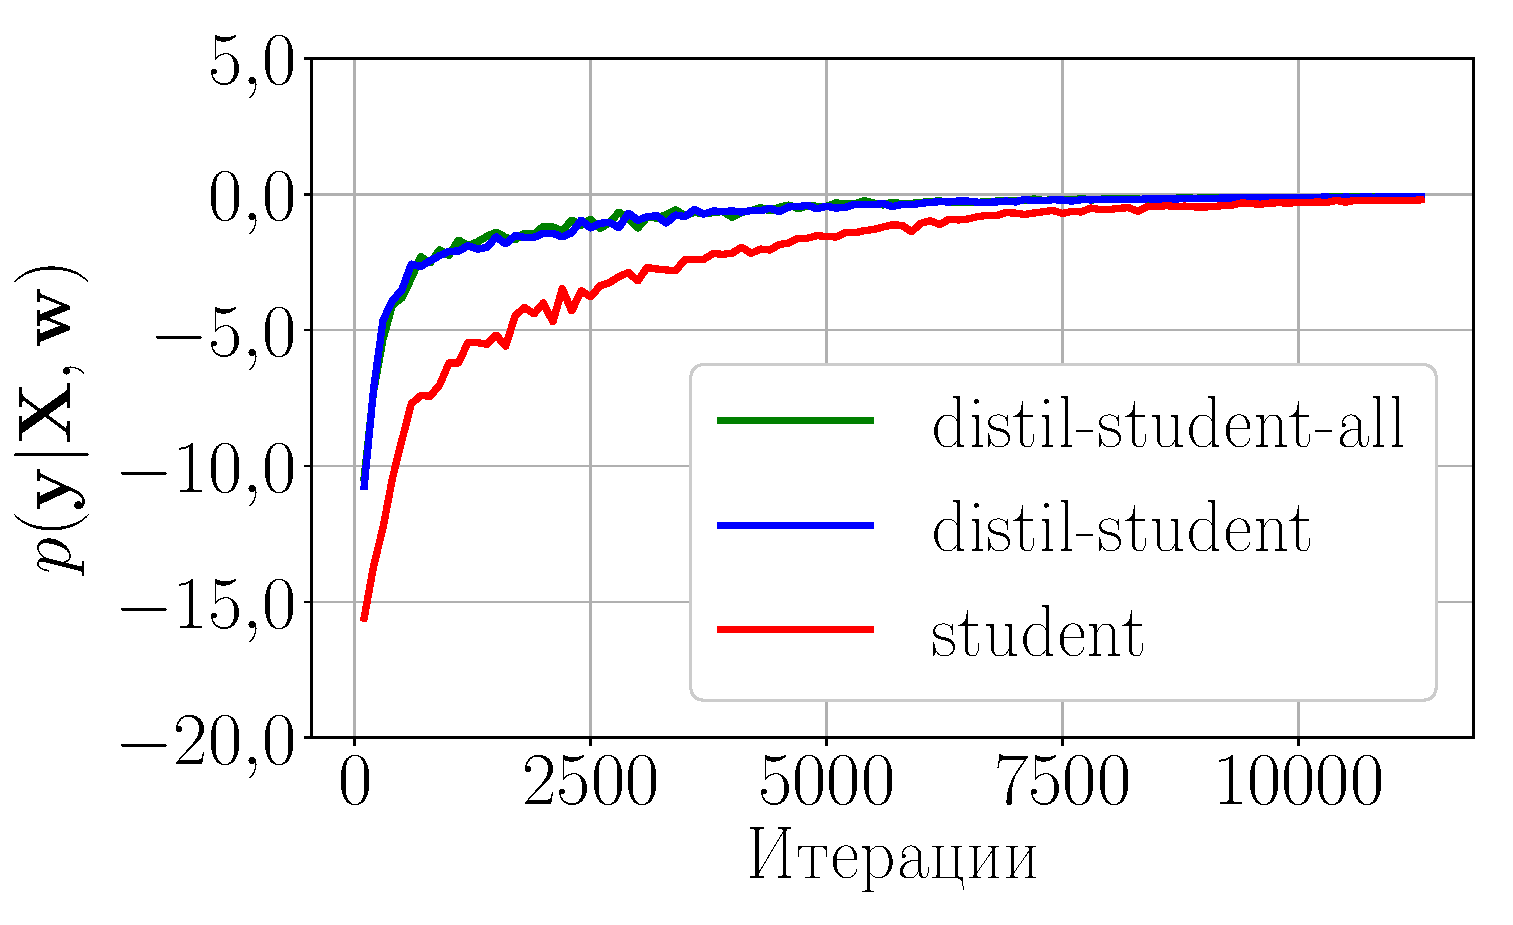
\includegraphics[width=0.5\textwidth]{results/bayesdistil/synthetic_likelihood_3_layers.eps}
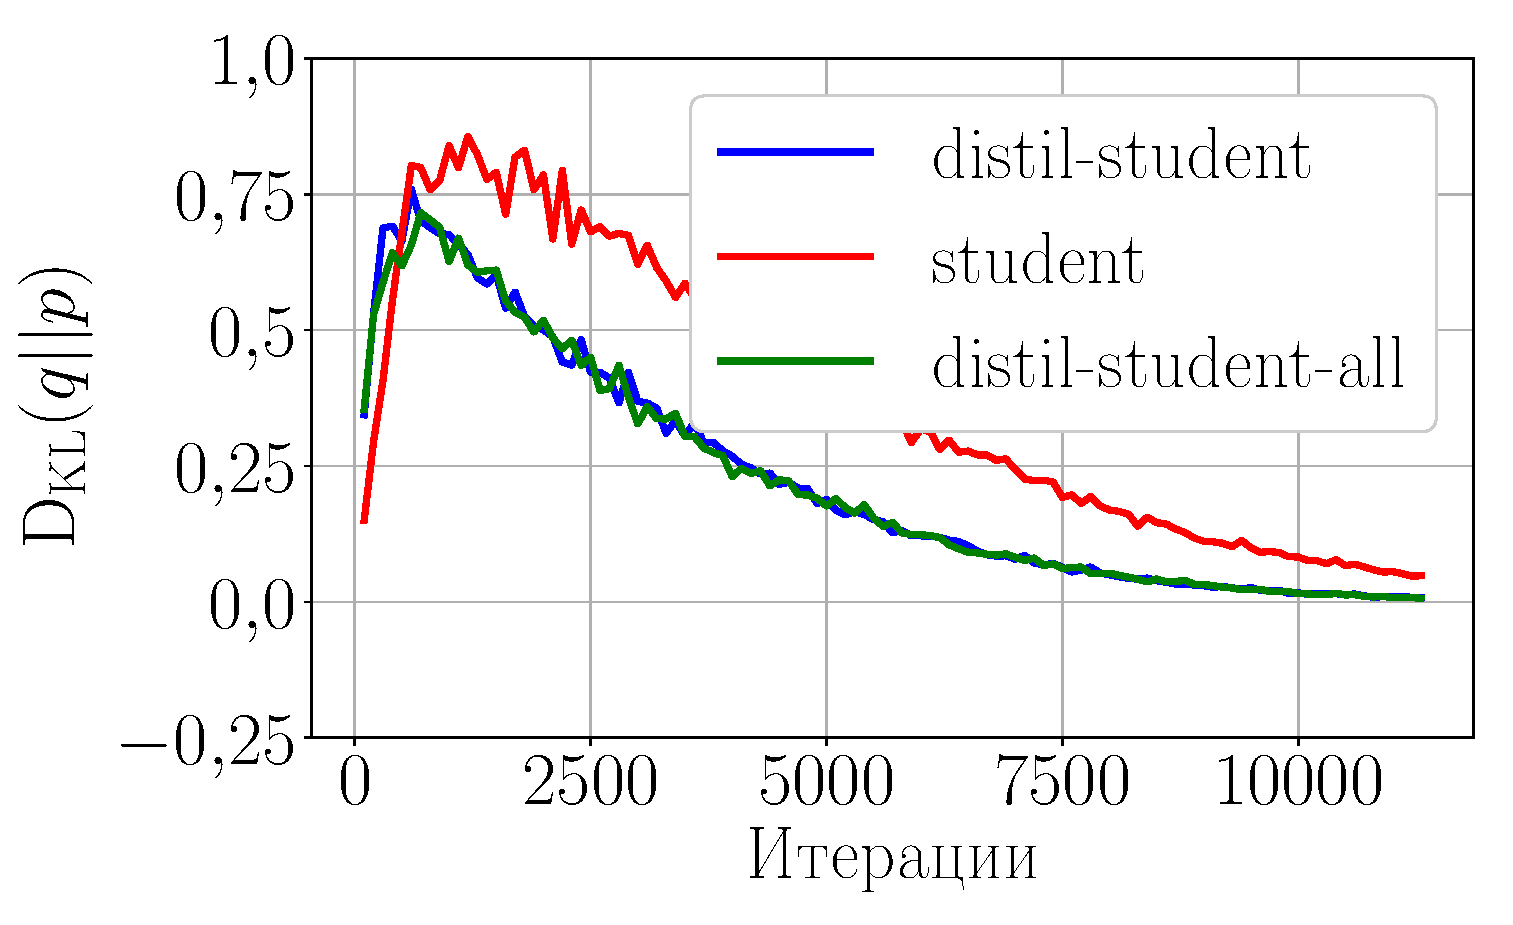
\includegraphics[width=0.5\textwidth]{results/bayesdistil/synthetic_D_KL_3_layers.eps}
\caption{Структура~\eqref{eq:ex:3} модели ученика $g$. Слева: правдоподобие выборки в зависимости от номера итерации при обучении. Справа: KL--дивергенция между вариационным и априорным распределениями параметров модели.}
\label{exp:fig1}
\end{figure}

Рис.~\ref{exp:fig1} сравнивает модели ученика, со структурой~\eqref{eq:ex:3}. Представлено сравнение разных моделей: модель без дистилляции, где в качестве априорного распределения выбирается стандартное нормальное распределение (на легенде обозначается student); модель с частичной дистилляцией, где в качестве среднего значения параметров выбираются параметры согласно выражения~\eqref{eq:ap:3}, а ковариационная матрица была приравнена к единичной матрицы (на легенде обозначается distil-student); модель с полной дистилляцией согласно выражения~\eqref{eq:ap:3} (на легенде обозначается distil-student-all). Видно, что модели ученика, где в качестве априорного распределения выбраны распределения, основанные на апостериорном распределение учителя имеют большее правдоподобие, чем модель где в качестве априорного распределения выбрано стандартное нормальное. Также заметим, что использования параметра среднего из апостериорного распределения дает основной вклад при дистилляции, так как качество моделей distil-student и distil-student-all совпадает.

Вторая конфигурация получается путем удаления слоя модели учителя:
\begin{gather}
\label{eq:ex:5}
\begin{aligned}
g = \bm{\sigma} \circ \mathbf{W}_2\bm{\sigma} \circ \mathbf{W}_1,
\end{aligned}
\end{gather}
где~$\bm{\sigma}$ является нелинейной функцией активации, а матрицы линейных преобразований имеют размер:
\begin{gather}
\label{eq:ex:6}
\begin{aligned}
\mathbf{W}_{1} \in \mathbb{R}^{1 \times 50}, \quad \mathbf{W}_{2} \in \mathbb{R}^{50 \times 10}.
\end{aligned}
\end{gather}
 В качестве функции активации была выбрана функция активации $\text{ReLu}$.

\begin{figure}[h!]
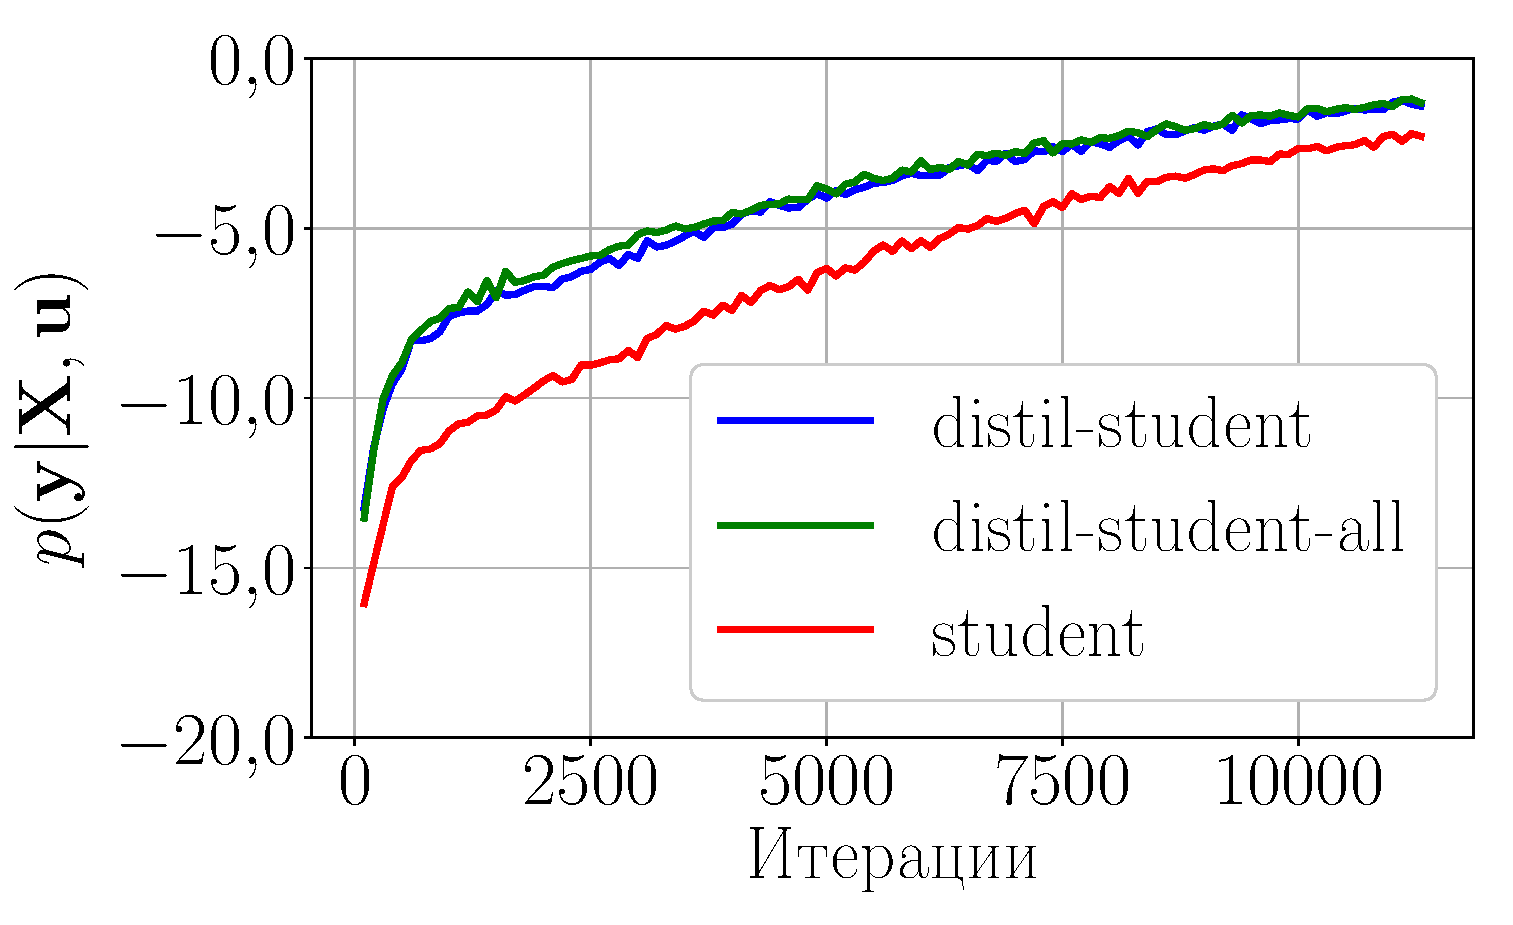
\includegraphics[width=0.5\textwidth]{results/bayesdistil/synthetic_likelihood_2_layers.eps}
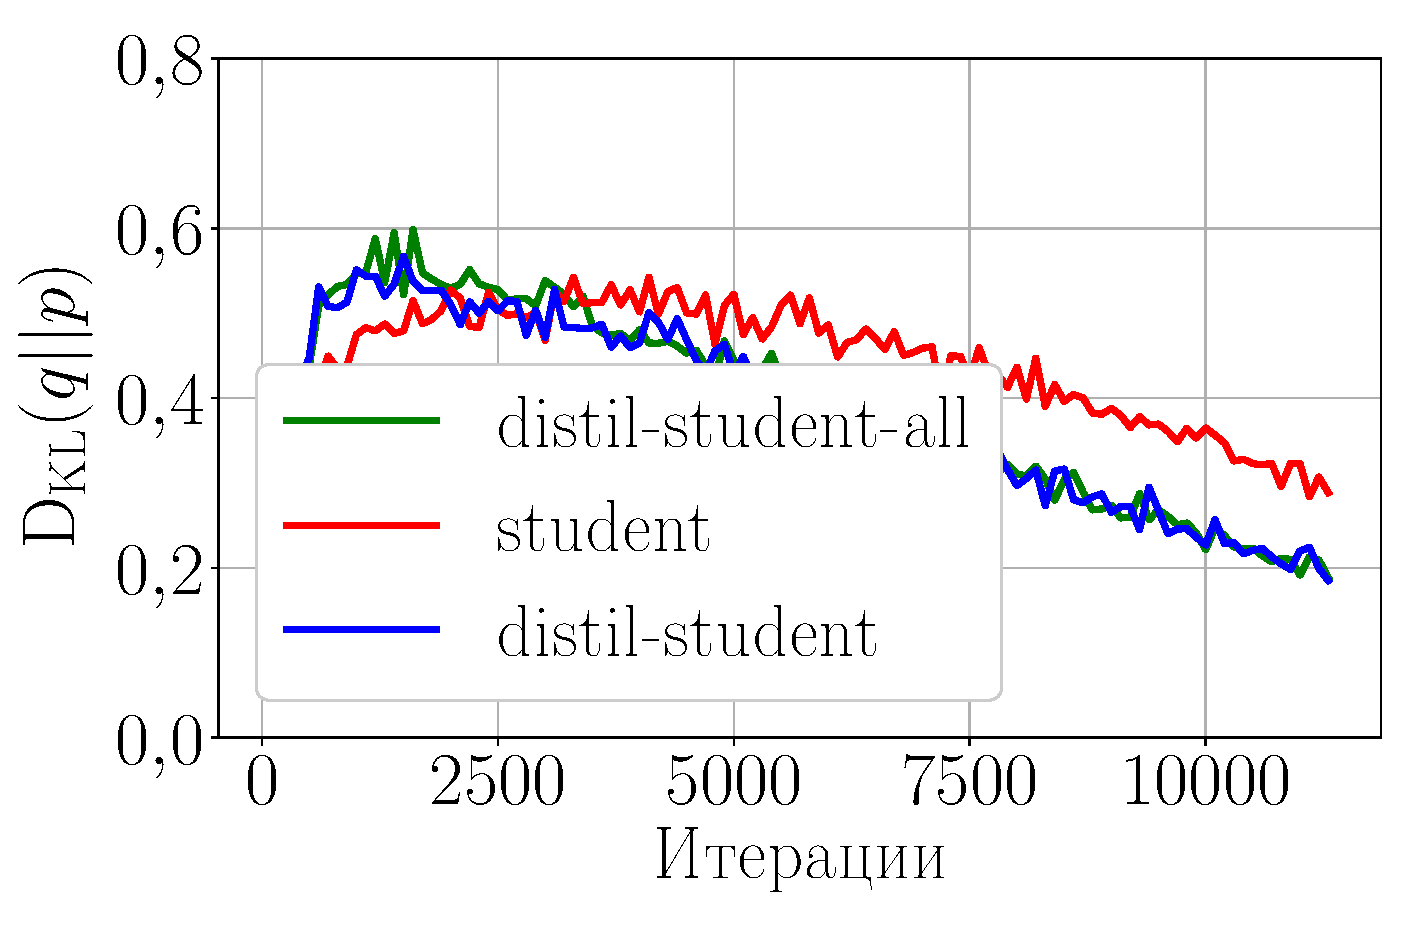
\includegraphics[width=0.5\textwidth]{results/bayesdistil/synthetic_D_KL_2_layers.eps}
\caption{Структура~\eqref{eq:ex:5} модели ученика~$g$. Слева: правдоподобие выборки в зависимости от номера итерации при обучении. Справа: KL--дивергенция между вариационным и априорным распределениями параметров модели.}
\label{exp:fig2}
\end{figure}

Рис.~\ref{exp:fig2} сравнивает модели ученика со структурой~\eqref{eq:ex:5}. Аналогично рис.~\ref{exp:fig1}, на рис.~\ref{exp:fig2} представлено сравнение модели без дистилляции (student), модели с дистилляцией параметра среднего значение (distil-student) и модели с полной дистилляцией (distil-student-all). В рамках данного эксперимента, по дистилляции модели учителя в модель ученика с меньшим числом параметров получены результаты, которые подтверждают, что задание априорного распределения параметров ученика позволяет улучшить число итераций при выборе оптимальных параметров модели ученика.

В рамках данного эксперимента проводился анализ байесовского подхода к дистилляции на реальных данных.  В качестве реальных данных выбрана выборка FashionMnist~\cite{fashionmnist} которая является задачей классификации изображений на 10 классов.

В качестве модели учителя рассматривалась модель многослойный перцептрон с двумя скрытыми слоями \eqref{eq:st:3}. Матрицы линейных преобразований имеют размер:
\begin{gather}
\label{eq:ex:7}
\begin{aligned}
\mathbf{U}_{1} \in \mathbb{R}^{800 \times 784}, \quad \mathbf{U}_{2} \in \mathbb{R}^{50 \times 800}, \quad \mathbf{U}_{3} \in \mathbb{R}^{10 \times 50},
\end{aligned}
\end{gather}
В качестве функции активации была выбрана функция активации $\text{ReLu}$.
Модель учителя предварительно обучена на основе вариационного вывода \eqref{eq:st:7}, где в качестве априорного распределения параметров выбрано стандартное нормальное распределение.

В качестве модели ученика были выбрана конфигурация с одним скрытым слоем~\eqref{eq:ex:5}, где матрицы линейных преобразований имеют размер:
\begin{gather}
\label{eq:ex:7}
\begin{aligned}
\mathbf{W}_{1} \in \mathbb{R}^{50 \times 784}, \quad \mathbf{W}_{2} \in \mathbb{R}^{50 \times 10}.
\end{aligned}
\end{gather}
В качестве функции активации была выбрана функция активации $\text{ReLu}$.

\begin{figure}[h!]
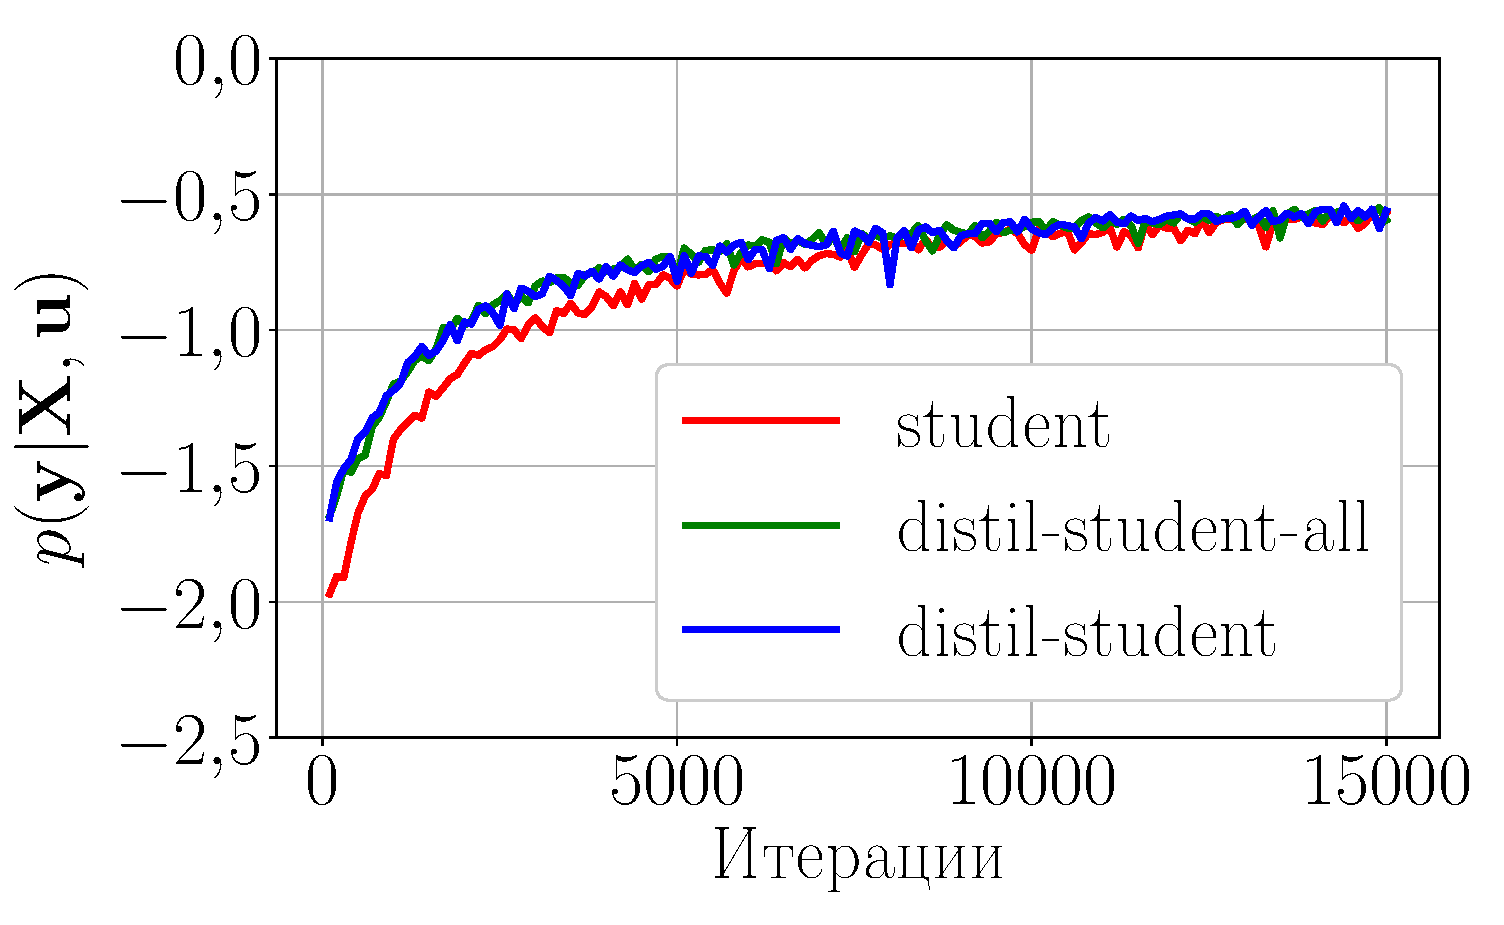
\includegraphics[width=0.5\textwidth]{results/bayesdistil/fashionmnist_likelihood_2_layers.eps}
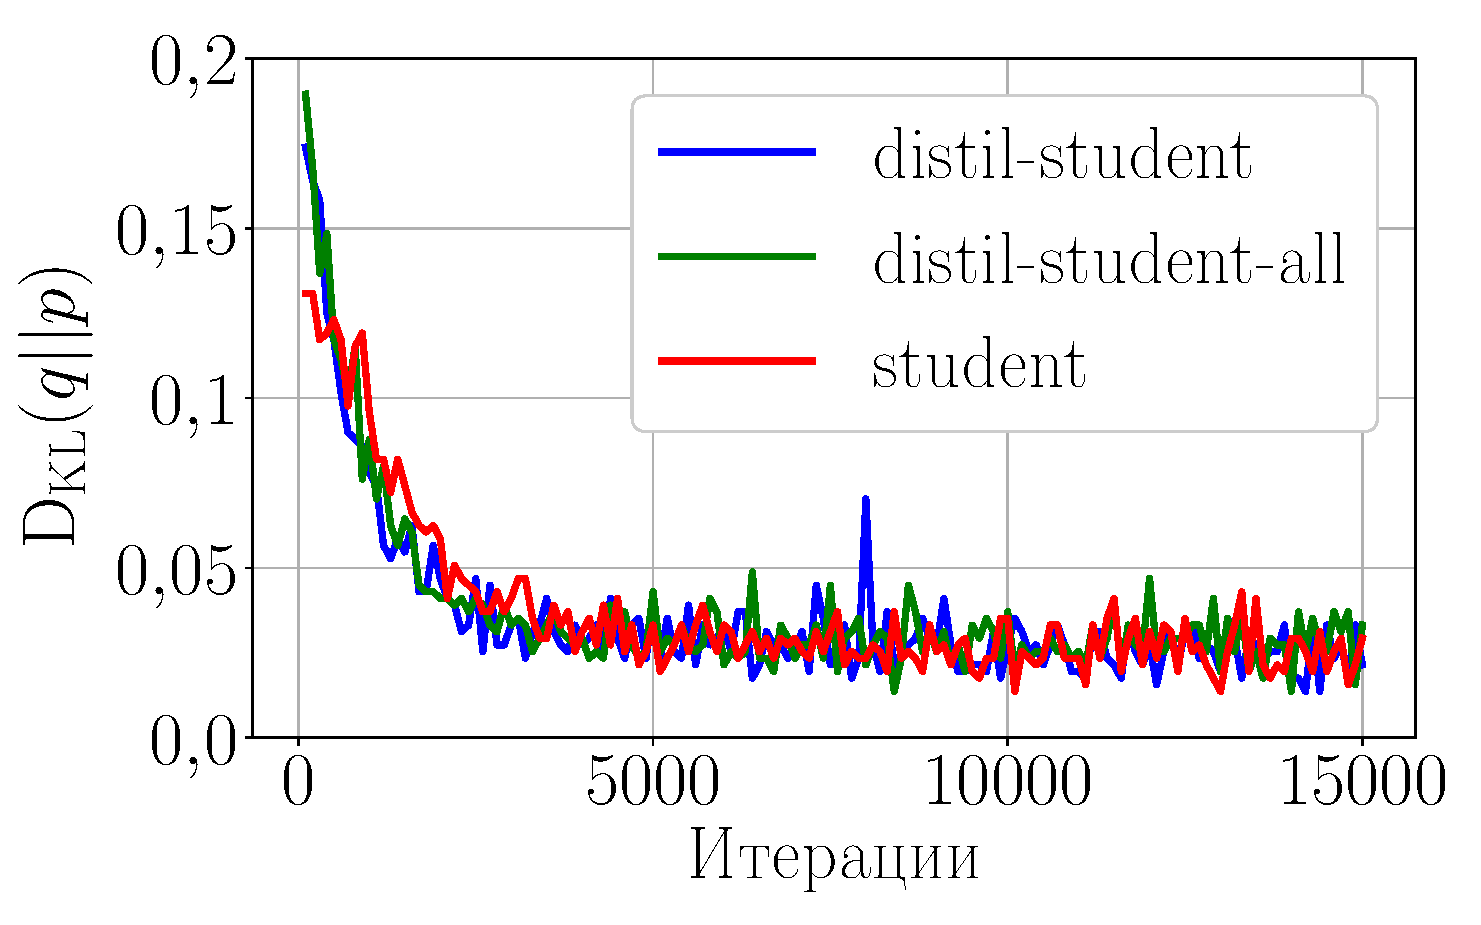
\includegraphics[width=0.5\textwidth]{results/bayesdistil/fashionmnist_D_KL_2_layers.eps}
\caption{Слева: правдоподобие выборки в зависимости от номера итерации при обучении. Справа: KL--дивергенция между вариационным и априорным распределениями параметров модели.}
\label{exp:fig3}
\end{figure}

Рис.~\ref{exp:fig3} сравнивает модели ученика с разными априорными распределениями параметров.
Аналогично синтетическому эксперименту, модель, где в качестве априорного распределения использовалось стандартное нормальное распределение, сравнивалась с моделью, где параметры распределения определялись на основе формулы~\eqref{eq:ap:5}. Видно, что у моделей с заданием априорного распределения на основе апостериорного распределения параметров учителя правдоподобие выборки выше, чем у модели, где в качестве априорного распределения выбрано стандартное нормальное распределение.

\begin{table}[]
\caption{Сводная таблица результатов вычислительного эксперимента.}
\label{tb:fn:1}
\begin{center}
\begin{tabular}{|l|c|c|c|c|llll}
\cline{1-5}
                 & teacher           & student        & distil-student & distil-student-all &                           &                      &                      &                      \\ \cline{1-5}
\multicolumn{5}{|c|}{Эксперимент на синтетической выборке (удаление нейрона)}             &                      &                      &                      &                      \\ \cline{1-5}
Структура            & $[10,100,50,1]$   & $[10,10,10,1]$  & $[10,10,10,1]$ & $[10,10,10,1]$    &                      &                      &                      &                      \\ \cline{1-5}
Число параметров  & 6050                    & 210                   & 210                  & 210                      &                      &                      &                      &                      \\ \cline{1-5}
Разность площадей   &   -                         & 0                       & 16559              & 16864                  &                      &                      &                      &                      \\ \cline{1-5}
\multicolumn{5}{|c|}{Эксперимент на синтетической выборке (удаление слоя)}                    & \multicolumn{1}{c}{} & \multicolumn{1}{c}{} & \multicolumn{1}{c}{} & \multicolumn{1}{c}{} \\ \cline{1-5}
Структура            & $[10,100,50,1]$   & $[10,50,1]$       & $[10,50,1]$      & $[10,50,1]$          &                      &                      &                      &                      \\ \cline{1-5}
Число параметров    &   6050                       &          550                &          550               &             550                &                      &                      &                      &                      \\ \cline{1-5}
Разность площадей~S    &  -                          &  0                      &  23310             & 25506                  &                      &                      &                      &                      \\ \cline{1-5}
\multicolumn{5}{|c|}{Эксперимент на выборке FashionMnist}                                                     &                      &                      &                      &                      \\ \cline{1-5}
Структура           & $[784,800,50,10]$& $[784,50,10]$   & $[784,50,10]$  & $[784,50,10]$      &                      &                      &                      &                      \\ \cline{1-5}
Число параметров    &           667700                  &          39700                &         39700                &                 39700            &                      &                      &                      &                      \\ \cline{1-5}
Разность площадей~S   & -                           & 0                       &  1165               & 1145                    &                      &                      &                      &                      \\ \cline{1-5}
\end{tabular}
\end{center}
\end{table}

В табл.~\ref{tb:fn:1} представлен результат вычислительного эксперимента. Для численного сравнения качества моделей выбрана разность площадей графика $p\bigr(\mathbf{y}|\mathbf{X}, \mathbf{u}\bigr)$ между моделью student и моделями distil-student  и 
distil-student-all соответсвенно:
\begin{gather}
\label{eq:ex:8}
\begin{aligned}
S = \sum_{s} p\bigr(\mathbf{y}|\mathbf{X}, \mathbf{u}^s_{\text{s}}\bigr) - p\bigr(\mathbf{y}|\mathbf{X}, \mathbf{u}^s_{\text{ds}}\bigr),
\end{aligned}
\end{gather}
где~$\mathbf{u}^s_{\text{s}}, \mathbf{u}^s_{\text{ds}}$ обозначает параметры модели студента и модели дистиллированного студента после~$s$-й итерации оптимизационного процесса. Заметим, что площадь~$S$ имеет знак: чем большее положительное число, тем дистиллированная модель лучше, чем модель построенная без учителя. В случае, если площадь~$S$ принимает отрицательное значение, то значит модель без дистилляции является лучше чем модель с дистилляцией. В рамках вычислительного эксперимента видно, что площадь~$S$ под графиками принимает положительные значения, то есть модели ученика полученные при помощи дистилляции являются лучше чем модель ученика без дистилляции.

\newpage

\section{Введение отношения порядка на множестве параметров аппроксимирующих моделей}
В данной работе предлагается метод введения отношения порядка на множестве параметров сложных параметрических моделей, таких как нейросеть. Рассматривается порядок, заданный при помощи ковариационной матрицы градиентов функции ошибки по параметрам модели \cite{Mandt2017}. В работе \cite{Chunyan2016} предложен итерационный метод для поиска ковариационной матрицы градиентов. Данный итерационный метод интегрируется в градиентный метод оптимизации Adam \cite{kingma2014}.

Множество параметров упорядочивается по возрастанию дисперсии: от параметра с минимальной дисперсией до параметра с максимальной дисперсией градиента функции ошибки по соответствующему параметру модели. Предполагается, что малая дисперсия градиента указывает на то, что соответствующий параметр можно зафиксировать.

Для задания порядка на множестве параметров при помощи ковариационной матрицы вводится предположение о том, что фиксация параметров происходит в момент, когда все параметры модели находятся в некоторой окрестности локального минимума функции ошибки. Данное условие накладывается для корректного использования итерационного метода поиска ковариационной матрицы градиентов.

Заданный порядок на множестве параметров модели используется для фиксации тех параметров модели, которые оказываются предстоящими с точки зрения заданного порядка. Сначала фиксируются те параметры, которые имеют минимальную дисперсию градиента в окрестности локального минимума функции ошибки.

Для анализа свойств предложенного метода задания порядка на множестве параметров проводился вычислительный эксперимент. В качестве моделей рассматривались модели различной структурной сложности: линейные модели, нейросетевые модели. Предложенный метод задания порядка сравнивается с методом, в котором порядок задан произвольным образом.
\subsection{Задача упорядочивания параметров аппроксимирующих моделей}
Задана выборка:
\[
\label{eq:st:1}
\begin{aligned}
\mathfrak{D} = \bigr\{\bigr(\textbf{x}_i, y_i\bigr)\bigr\}_{i=1}^{m}, \quad \textbf{x}_{i} \in \mathbb{X} = \mathbb{R}^{n}, \quad y_i \in \mathbb{Y},
\end{aligned}
\]
где $n$ --- размерность признакового пространства, $m$ --- число объектов в выборке. Пространство ответов $\mathbb{Y} = \mathbb{R}$ в случае задачи регрессии и  $\mathbb{Y} = \{1,\cdots, K\}$ в случае задачи классификации, где $K$ --- число классов.

Задано семейство моделей параметрических функций с наперед заданной структурой:
\[
\label{eq:st:2}
\begin{aligned}
\mathfrak{F} &= \bigr\{f\bigr(\textbf{w}\bigr):\mathbb{X} \to \mathbb{Y} | \textbf{w} \in \mathbb{R}^{p}\bigr\}, \\ 
\mathbf{h}\bigr(\textbf{w}, \textbf{x}\bigr) &= \textbf{W}_1\bm{\sigma}\bigr(\textbf{W}_2\bm{\sigma}\bigr(\cdots\bm{\sigma}\bigr(\textbf{W}_r\textbf{x}\bigr)\cdots\bigr)\bigr),\\
f_{\text{\text{cl}}}\bigr(\textbf{w}, \textbf{x}\bigr) &= \arg \max_{j \in \bigr\{1,\cdots, K\bigr\}} \text{softmax}\bigr(\mathbf{h}\bigr(\textbf{w}, \textbf{x}\bigr)\bigr)_{j}, \\ 
f_{\text{reg}}\bigr(\textbf{w}, \textbf{x}\bigr) & = \mathbf{h}\bigr(\textbf{w}, \textbf{x}\bigr), 
\end{aligned}
\]
где $p$ --- размерность пространства параметров, $r$ --- число слоев нейросети, $\textbf{w} = \text{vec}[\textbf{W}_1, \textbf{W}_2, \cdots, \textbf{W}_r]$, а $\bm{\sigma}$ --- функция активации. В случае задачи регрессии структура модели имеет вид $f_{\text{\text{reg}}}$, а в случае классификации имеет вид $f_{\text{\text{cl}}}$.
%В качестве $\tau$ рассматривается $\tau\bigr(\textbf{x}\bigr) = \textbf{x}$ в случае задачи регрессии, в случае задачи многоклассовой классификации $\bm{\sigma}\bigr(\textbf{x}\bigr) = \text{softmax}\bigr(\textbf{x}\bigr)$.
Задана функция потерь:
\[
\label{eq:st:3}
\begin{aligned}
\mathcal{L}\bigr(\textbf{w}, \mathfrak{D}\bigr) &= \frac{1}{m}\sum_{i=1}^{m}l\bigr(\textbf{x}_{i}, y_i, \textbf{w}\bigr),\\
l_{\text{\text{reg}}}\bigr(\textbf{x}, y, \textbf{w}\bigr) &= \bigr(y - f\bigr(\textbf{w}, \textbf{x}\bigr)\bigr)^{2},\\
l_{\text{\text{cl}}}\bigr(\textbf{x}, y, \textbf{w}\bigr) &= -\sum_{j=1}^{K}\bigr([y = j]\ln\text{softmax}_j\bigr(\mathbf{h}\bigr(\textbf{w}, \textbf{x}\bigr)\bigr)\bigr),
\end{aligned}
\]
где $l_{\text{\text{reg}}}$ --- это функция ошибки на одном элементе для задачи регрессии, $l_{\text{\text{cl}}}$ --- для задачи классификации.
Оптимальный вектор параметров $\hat{\textbf{w}}$ получим минимизацией функции потерь:
\[
\label{eq:st:0:1}
\begin{aligned}
\hat{\textbf{w}} = \arg \min_{\textbf{w}\in\mathbb{R}^{p}} \mathcal{L}\bigr(\textbf{w}, \mathfrak{D}\bigr).
\end{aligned}
\]

Для поиска оптимальных параметров модели используется градиентный метод оптимизации:
\[
\label{eq:st:4}
\begin{aligned}
\textbf{w}_{t} = \textbf{w}_{t-1} + \Delta\textbf{w}\bigr(\textbf{g}_{S,t}, \textbf{w}_{t-1}, \textbf{w}_{t-2}, \cdots\bigr), \quad \textbf{g}_{S,t}=\frac{\partial \mathcal{L}\bigr(\textbf{w}_{t}, \textbf{X}_{S}, \textbf{Y}_{S}\bigr)}{\partial \textbf{w}},
\end{aligned}
\]
где $t$ --- номер итерации, $\textbf{g}_{S,t}$ --- значение градиента на подвыборке размера $S$, $\Delta\textbf{w}$ --- приращение вектора параметров.
 
 
Порядок на множестве параметров модели задается при помощи ковариационной матрицы $\textbf{C}$ градиентов функции ошибки $\mathcal{L}$ по параметрам модели $\textbf{w}$. Для вычисления ковариационной матрицы $\textbf{C}$ используется итерационная формула \cite{Chunyan2016}, которая вычисляется на каждой итерации \eqref{eq:st:4} градиентного метода оптимизации параметров:
\[
\label{eq:st:5}
\begin{aligned}
\textbf{C}_t = \bigr(1-\kappa_t\bigr)\textbf{C}_{t-1}+\kappa_t\bigr(\textbf{g}_{1,t}-\textbf{g}_{S,t}\bigr)\bigr(\textbf{g}_{1,t}-\textbf{g}_{S,t}\bigr)^{\mathsf{T}},
\end{aligned}
\]
 где $t$ --- номер итерации, $\textbf{g}_{S,t}$ --- значение градиента на подвыборке размера $S$, $\textbf{g}_{1,t}$ --- значение градиента на первом элементе подвыборки, $\kappa_t=\frac{1}{t}$ --- параметр сглаживания, $\textbf{C}_0$ инициализируются из равномерного распределения.
 
Пусть известно $t_0$ --- число итераций, после которого все параметры находятся в некоторой локальной окрестности минимума, тогда, как показано в работе \cite{Chunyan2016}, матрица $\textbf{C}_{t_0}$ аппроксимирует истинную ковариационную матрицу $\textbf{C}$. Ковариационная матрица $\textbf{C}_{t_0}$ используется для упорядочения параметров модели $\textbf{w}_{t_0}$. 
 
Пусть $\mathcal{I}$ ---  упорядоченный вектор индексов $[1, 2, \cdots, p]$. Обозначим $\mathcal{I}_{\textbf{w}_{t_0}}$ вектор индексов, порядок которого задан при помощи ковариационной матрицы $\textbf{C}_{t_0}$. 
 
Например, если ковариационная матрица $\textbf{C}_{t_0}$  имеет вид
 $$
\begin{bmatrix}
0{,}3& 0 & 0\\
0& 0{,}2 & 0\\
0& 0 & 0{,}25\\
\end{bmatrix},
 $$
 то вектор индексов $\mathcal{I}_{\textbf{w}_{t_0}} = [3,1,2]$.
 

\subsection{Фиксация параметров модели в процессе обучения}
Для фиксации параметров $\textbf{w}_{t_0}$ при помощи вектора индексов $\mathcal{I}_{\textbf{w}_{t_0}}$ используется бинарный вектор $\bm{\alpha}\bigr(k\bigr)$:
\[
\label{eq:st:6}
\begin{aligned}
\alpha_i\bigr(k\bigr) = \begin{cases}
   1, &\text{если }\mathcal{I}_{\textbf{w}_{t_0}}[j] \leq k;\\
   0 &\text{иначе},
 \end{cases}
\end{aligned}
\]
 где $k$ --- число фиксирующих параметров.
 
 Учитывая \eqref{eq:st:6}, уравнение \eqref{eq:st:4} приводится к виду
 \[
\label{eq:st:7}
\begin{aligned}
\textbf{w}_{t} = \textbf{w}_{t-1} + \bm{\alpha}\bigr(k\bigr)\cdot\Delta\textbf{w}\bigr(\textbf{g}_{S,t}, \textbf{w}_{t-1}, \textbf{w}_{t-2}, \cdots\bigr),
\end{aligned}
\]
где $t$ --- номер итерации, $\textbf{g}_{S,t}$ --- значение градиента на подвыборке размера $S$, $\Delta\textbf{w}$ --- приращение вектора параметров. После умножения на бинарный вектор $\bm\alpha$ часть параметров не оптимизируется, что приводит к фиксации параметров.

\subsection{Вычислительный эксперимент по упорядочиванию параметров}

\begin{table}[h!t]
\begin{center}
\caption{Описание выборок, используемых в эксперименте}
\label{tb:ex:1}
\begin{tabular}{|c|c|c|c|c|c|}
\hline
	Выборка, $\mathfrak{D}$& Тип & Число& Модель& Число \\
	&& признаков, $n$&&параметров, $p$\\
	\hline
	\multicolumn{1}{|l|}{Boston Housing}&
	Регрессия& 13& Нейросеть& 301\\
	\hline
	\multicolumn{1}{|l|}{MNIST}&
	Классификация& 784& Нейросеть& 7960\\
	\hline
	\multicolumn{1}{|l|}{Synthetic 3}&
	Регрессия& 200& Линейная& 200\\
	\hline
	\multicolumn{1}{|l|}{Synthetic 2}&
	Классификация& 200& Линейная& 200\\
	\hline
	\multicolumn{1}{|l|}{Synthetic 1}&
	Регрессия& 200& Нейросеть& 4041\\
\hline

\end{tabular}
\end{center}
\end{table}

Для анализа результатов, полученных предложенным алгоритмом, проводится вычислительный эксперимент. В качестве данных используются синтетические и реальные данные, которые описаны в табл. \ref{tb:ex:1}. Выборки MNIST \cite{mnist} и Boston Housing \cite{Boston} рассматриваются в качестве реальных данных, для которых решается задача классификации и регрессии соответственно. Синтетические выборки задаются следующим образом:
\[
\label{eq:ex:1}
\begin{aligned}
\mathfrak{D}_{\text{\text{reg}}} &= \bigr\{\bigr(\textbf{x}_i, y_i \bigr) |\textbf{x}_{i}\sim\mathcal{N}\bigr(\textbf{0}, \textbf{I}_{n}\bigr), y_{i}\sim\mathcal{N}\bigr(\textbf{w}^{\mathsf{T}}\textbf{x}_{i}, \textbf{I}_{n}\bigr),  \textbf{w} \sim \mathcal{N}\bigr(\textbf{0}, \textbf{I}_{n}\bigr)\bigr\},\\
\mathfrak{D}_{\text{\text{cl}}} &= \bigr\{\bigr(\textbf{x}_i, y_i \bigr) |\textbf{x}_{i}\sim\mathcal{N}\bigr(\textbf{0}, \textbf{I}_{n}\bigr), y_{i}\sim\mathcal{B}e\bigr(\textbf{w}^{\mathsf{T}}\textbf{x}_{i}\bigr),  \textbf{w} \sim \mathcal{N}\bigr(\textbf{0}, \textbf{I}_{n}\bigr)\bigr\}.
\end{aligned}
\]

В качестве аппроксимирующих моделей рассматриваются линейные и нейросетевые модели \eqref{eq:st:2}. В качестве функции ошибки для задачи регрессии рассматривается MSELoss, а для задачи классификации --- CrossEntropyLoss \eqref{eq:st:3}.

Предварительно для каждой модели и выборки определяется число $t_0$ --- номер итерации, после которой все параметры модели находятся в некоторой окрестности локального минимума. Параметр $t_0$ устанавливается экспериментальным путем для каждой модели и выборки отдельно из условия, что качество модели меняется незначительно при числе итераций $t>t_0$.

После $t_0$ шагов алгоритма оптимизации часть параметров модели фиксируется в соответствии с формулами \eqref{eq:st:6}, \eqref{eq:st:7}. Результат работы получается усреднением по $25$ независимым запускам оптимизации модели. Значение функции ошибки $\mathcal{L}$ усредняется по разным запускам алгоритма оптимизации. В ходе эксперимента проводится анализ вектора $\bm{\alpha}$, который также усредняется по разным запускам алгоритма оптимизации. Усредненное значение бинарного вектора  $\bm{\alpha}$ обозначим $\hat{\bm{\alpha}}$.

%Эксперимент состоит из трех этапов. На первом этапе проводится оптимизация модели, проделав $\eta_0$ итераций градиентного метода \eqref{eq:st:4}, для поиска параметров близких к оптимуму, а также поиска ковариационной матрицы $\textbf{C}_{\eta_0}$. На втором этапе проводится выбор $k$ параметров для фиксации параметров при помощи ковариациионной матрицы $\textbf{C}_{\eta_0}$. На третьем этапе проводится оптимизация параметров, которые не были зафиксированы.

\paragraph{Выборка Synthetic 1.}

\begin{figure}[h!t]\center
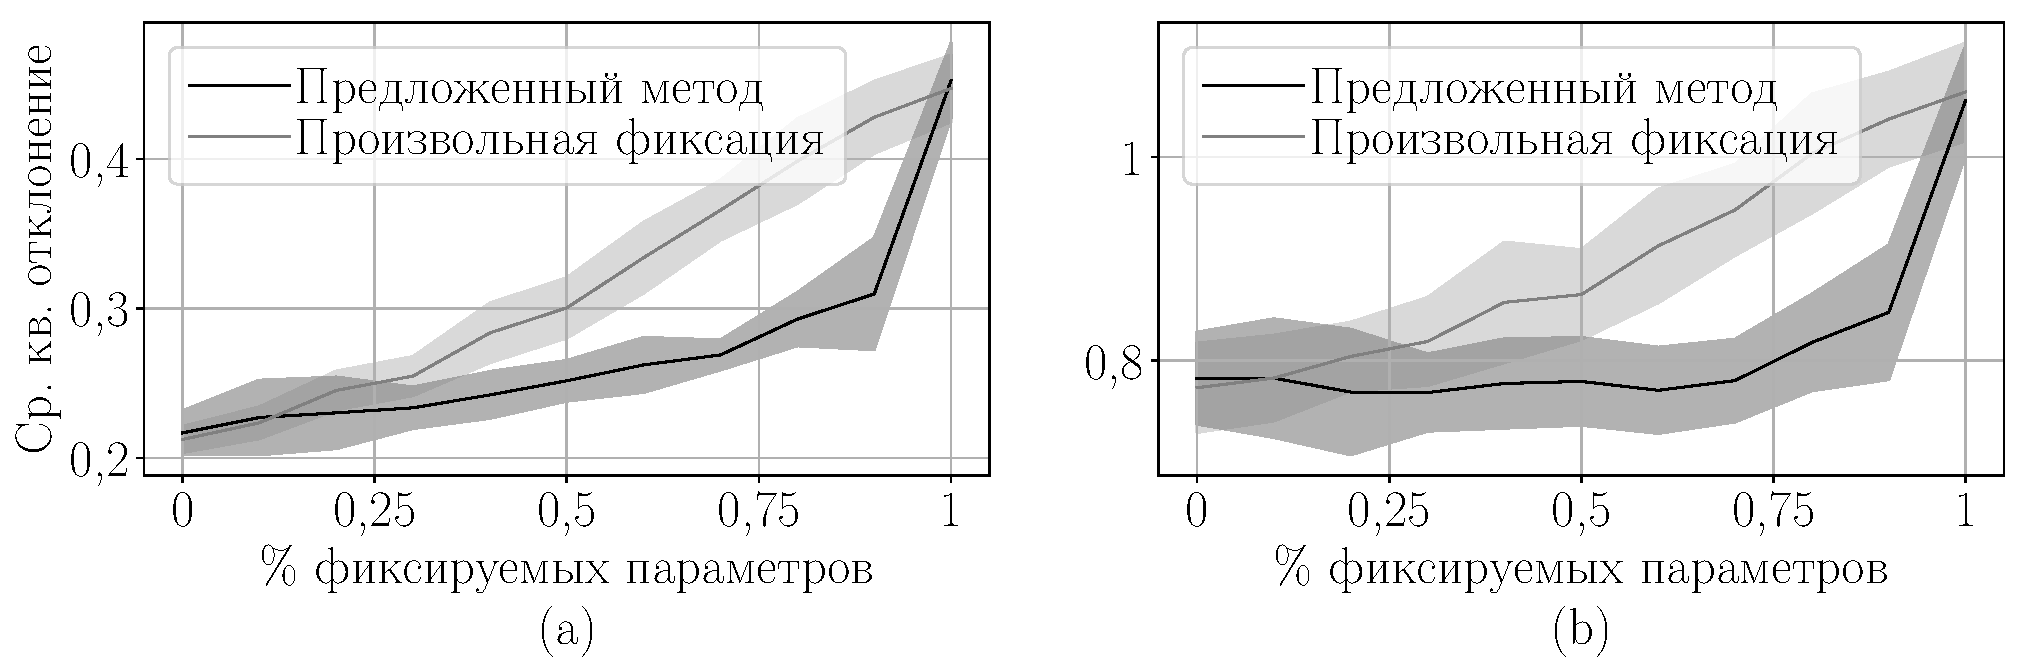
\includegraphics[width=1\textwidth]{results/order/generate_data_neural_loss}
\caption{Зависимость качества модели от числа зафиксированных параметров: a) на обучающей выборке; b) на тестовой выборке}
\label{fg:ex:syn3:1}
\end{figure}

\begin{figure}[h!t]\center
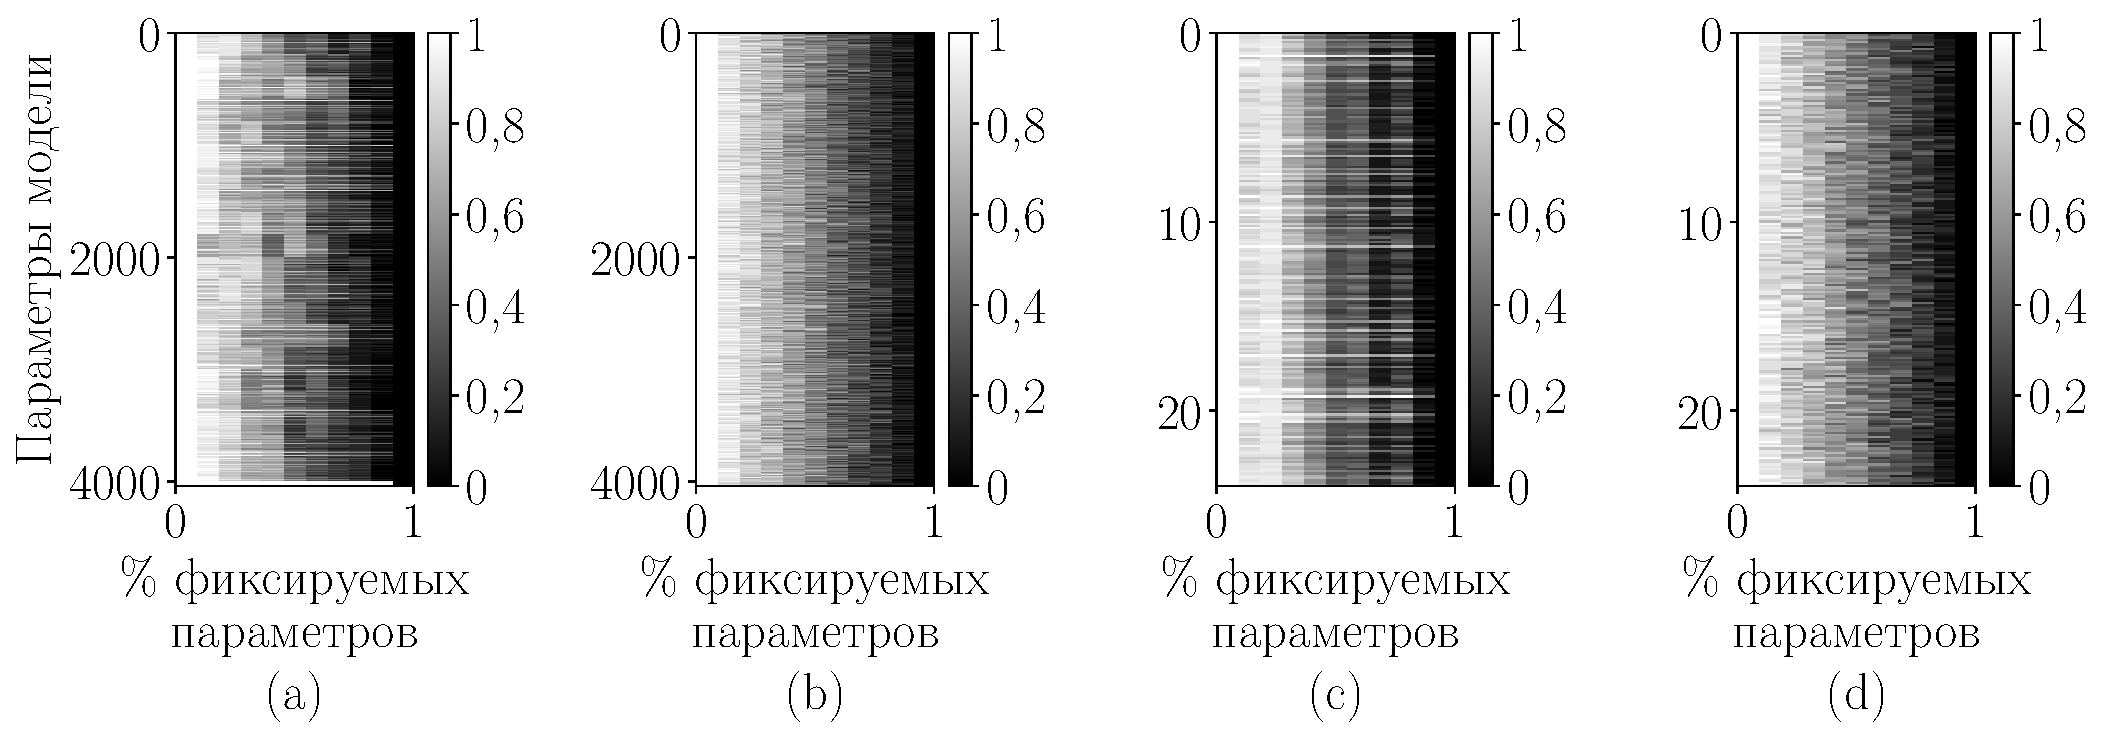
\includegraphics[width=1\textwidth]{results/order/generate_data_neural_matshow}
\caption{Визуализация векторов $\hat{\bm{\alpha}}\bigr(k\bigr)$ в зависимости от числа фиксируемых параметров: a) все параметры модели упорядочены предложенным методом; b) все параметры модели упорядочены произвольным образом; c) часть параметров модели упорядочена предложенным методом; d) часть параметров модели упорядочена произвольным образом}
\label{fg:ex:syn3:2}
\end{figure}

Эксперимент проводился на синтетически построенных данных. В качестве модели использовалась двухслойная нейросеть --- перцептрон.
%На рис. \ref{fg:ex:syn3:1} показано, что фиксация параметров в соответствии с предложенным порядком является лучше, чем фиксация параметров произвольным образом, так как функция ошибки растет медленней при фиксации большего процента параметров.
На рис. \ref{fg:ex:syn3:1} показаны графики зависимости функции потерь $\mathcal{L}$ от числа фиксируемых параметров. В случае фиксации параметров предложенным методом функция потерь $\mathcal{L}$ растет медленней, чем в случае фиксации параметров произвольным образом.

На рис. \ref{fg:ex:syn3:2} показана зависимость векторов $\hat{\bm{\alpha}}\bigr(k\bigr)$ от числа фиксируемых параметров. Каждый столбец соответствует одному вектору $\hat{\bm{\alpha}}\bigr(k\bigr)$. На рис. \ref{fg:ex:syn3:2}a, \ref{fg:ex:syn3:2}с видно, что $\hat{\bm{\alpha}}\bigr(k\bigr)$ имеет большое число компонент вектора, близких к $1$. Так как $\hat{\bm{\alpha}}\bigr(k\bigr)$ является усреднением вектора с компонентами $0$ или $1$, то предложенный порядок задает некоторый устойчивый порядок на множестве параметров модели. На рис. \ref{fg:ex:syn3:2}b, \ref{fg:ex:syn3:2}d видно, что в случае произвольной фиксации параметров компоненты вектора $\hat{\bm{\alpha}}\bigr(k\bigr)$ имеют одинаковые значения, следовательно, никакого порядка на множестве параметров нет.

\paragraph{Выборка Boston Housing.}
\begin{figure}[h!t]\center
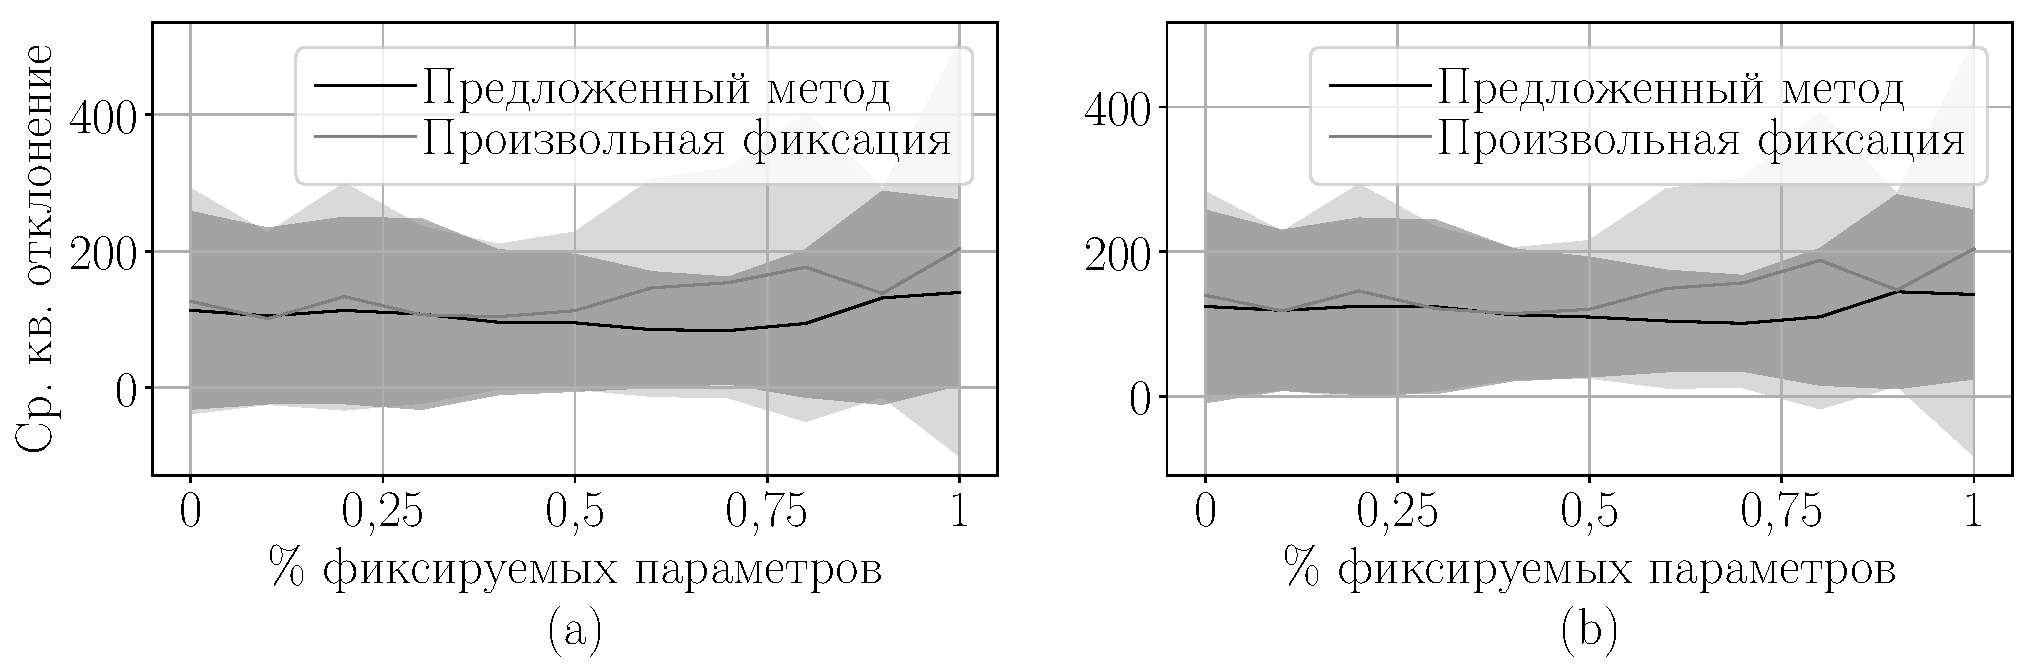
\includegraphics[width=1\textwidth]{results/order/boston_data_loss}
\caption{Зависимость качества модели от числа зафиксированных параметров: a) на обучающей выборке; b) на тестовой выборке}
\label{fg:ex:bost:1}
\end{figure}
Эксперимент проводился на реальных данных.
%На рис. \ref{fg:ex:bost:1} показано, что фиксация параметров в соответствии с предложенным порядком является лучше, чем заморозка параметров произвольным образом, так как функция ошибки растет медленней при фиксации параметров. Также видно, что в случае произвольной фиксации параметров функция ошибки имеет большую дисперсию, что указывает на сильную не устойчивость. Фиксация параметров предложенным методом является более устойчивым, что следует из того, что функция ошибки имеет меньше дисперсию.
На рис. \ref{fg:ex:bost:1} показаны графики зависимости функции потерь $\mathcal{L}$ от числа фиксируемых параметров. В случае фиксации параметров предложенным методом, функция потерь $\mathcal{L}$ растет так же, как и в случае фиксации параметров произвольным образом.
Данный результат следует из того, что нейросеть оказалась избыточно сложной моделью с большим числом параметров. После фиксации значимого числа параметров у модели оставалась большое число параметров для дообучения.

На рис. \ref{fg:ex:bost:2} показана зависимость векторов $\hat{\bm{\alpha}}\bigr(k\bigr)$ от числа фиксируемых параметров. На рис. \ref{fg:ex:bost:2}a, \ref{fg:ex:bost:2}с видно, что $\hat{\bm{\alpha}}\bigr(k\bigr)$ меняется незначительно от запуска к запуску алгоритма. Следовательно, предложенный порядок задает устойчивый к разным запускам порядок на множестве параметров модели. На рис. \ref{fg:ex:bost:2}b, \ref{fg:ex:bost:2}d видно, что в случае произвольной фиксации параметров вектор $\hat{\bm{\alpha}}\bigr(k\bigr)$ является произвольным и никакого порядка на множестве параметров нет.

\begin{figure}[h!t]\center
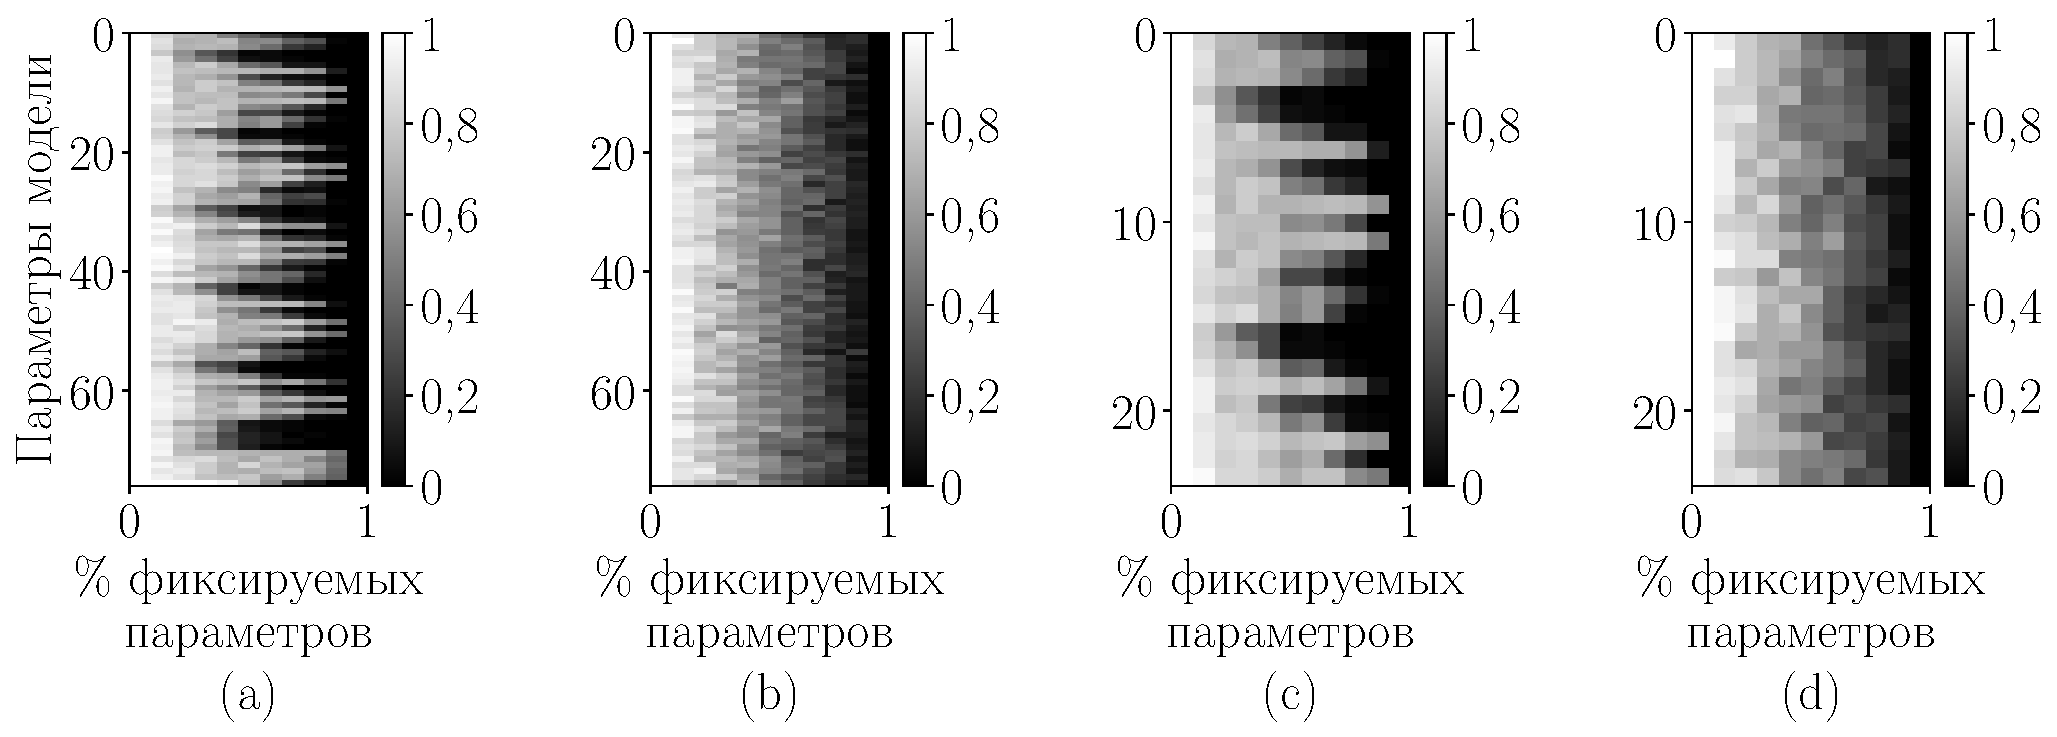
\includegraphics[width=1\textwidth]{results/order/boston_data_matshow}
\caption{Визуализация векторов $\hat{\bm{\alpha}}\bigr(k\bigr)$ в зависимости от числа фиксируемых параметров: a) все параметры модели упорядочены предложенным методом; b) все параметры модели упорядочены произвольным образом; c) часть параметров модели, упорядочена предложенным методом; d) часть параметров модели упорядочена произвольным образом}
\label{fg:ex:bost:2}
\end{figure}

\paragraph{Выборка Synthetic 3.}
\begin{figure}[h!t]\center
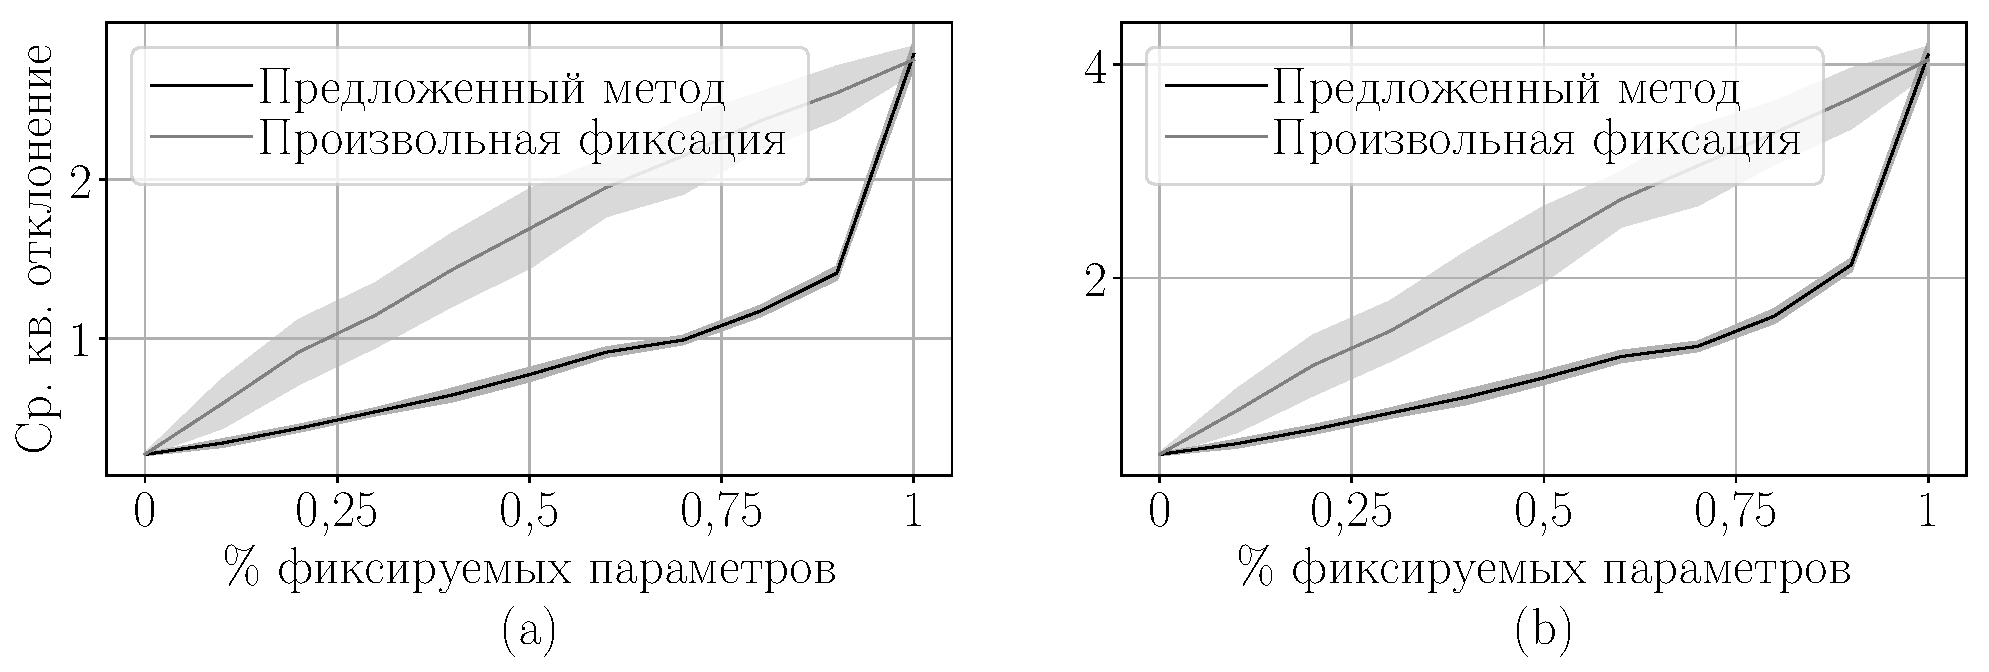
\includegraphics[width=1\textwidth]{results/order/generate_data_linear_loss}
\caption{Зависимость качества модели от числа зафиксированных параметров: a) на обучающей выборке; b) на тестовой выборке}
\label{fg:ex:syn1:1}
\end{figure}

\begin{figure}[h!t]\center
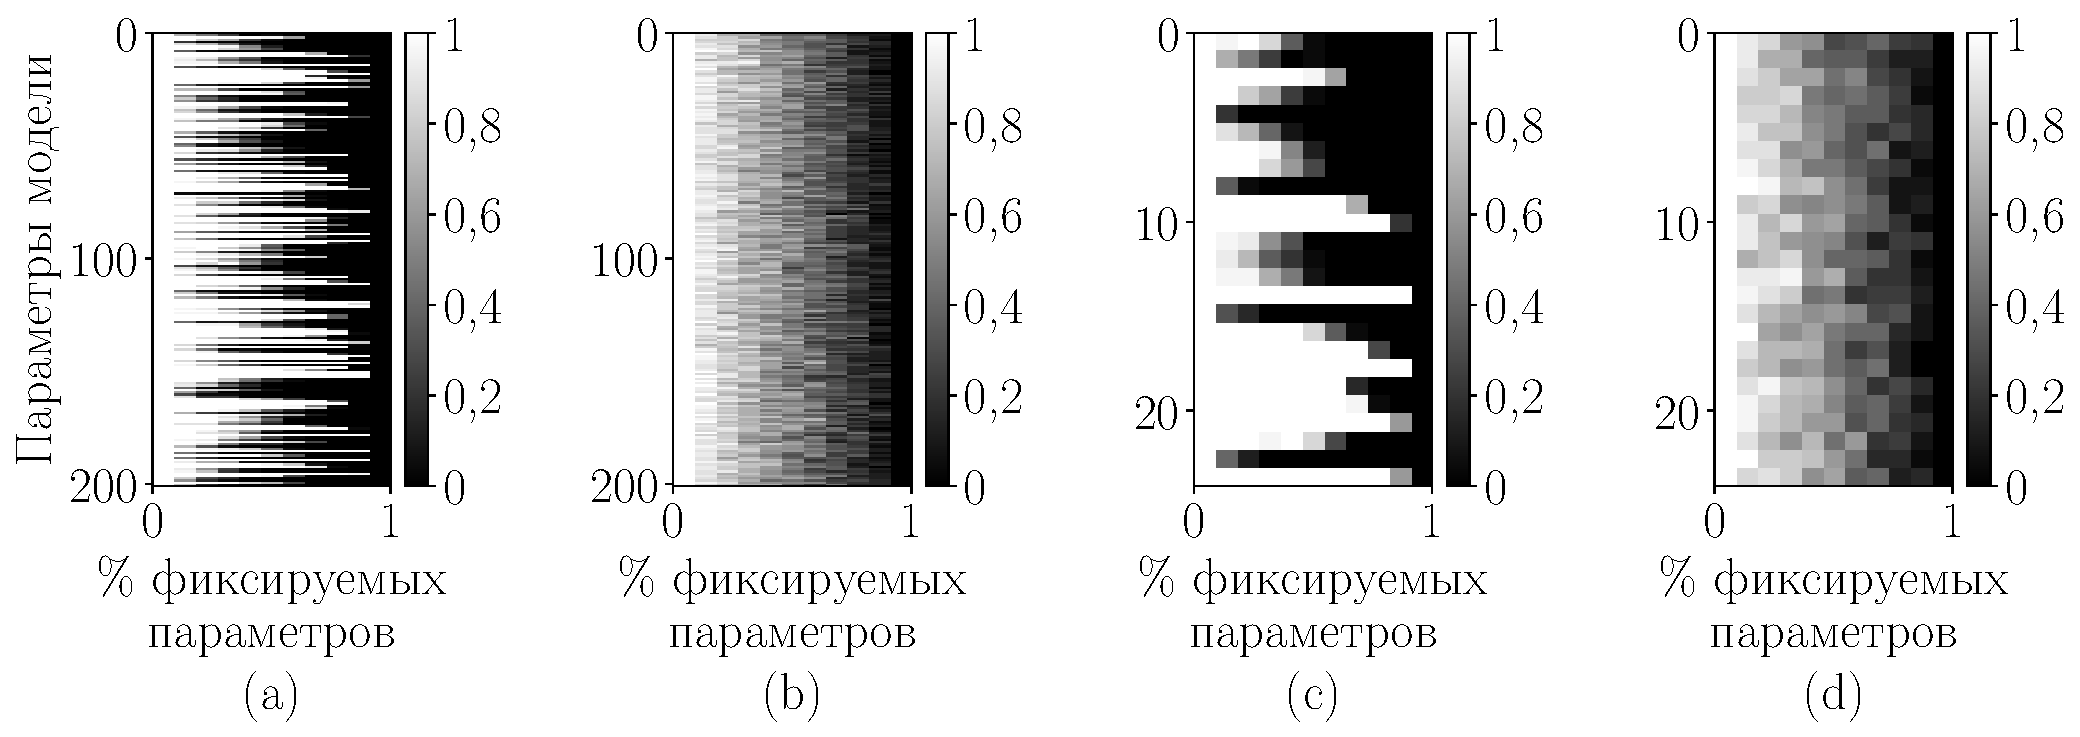
\includegraphics[width=1\textwidth]{results/order/generate_data_linear_matshow}
\caption{Визуализация векторов $\hat{\bm{\alpha}}\bigr(k\bigr)$ в зависимости от числа фиксируемых параметров: a) все параметры модели упорядочены предложенным методом; b) все параметры модели упорядочена произвольным образом; c) часть параметров модели, упорядочены предложенным методом; d) часть параметров модели упорядочена произвольным образом}
\label{fg:ex:syn1:2}
\end{figure}

Эксперимент проводился на синтетически построенных данных. В качестве модели использовалась линейная модель регрессии.
%На рис. \ref{fg:ex:syn1:1} показано, что фиксация параметров в соответсвии с предложенным порядком является лучше, чем фиксация параметров произвольным образом, так как функция ошибки растет медленней при фиксации параметров. Фиксация параметров предложенным методом является более устойчивым, что следует из того, что дисперсия функции ошибки почти отсутствует в отличии от дисперсии функции ошибки, где фиксация параметров производилась произвольным образом.
На рис. \ref{fg:ex:syn1:1} показаны графики зависимости функции потерь $\mathcal{L}$ от числа фиксируемых параметров. В случае фиксации параметров предложенным методом функция потерь $\mathcal{L}$ растет значительно медленней в сравнении со случаем фиксации параметров произвольным образом. Дисперсия функции ошибки также значительно меньше в случае фиксации параметров предложенным методом.

На рис. \ref{fg:ex:syn1:2} показано, что вектора $\hat{\bm{\alpha}}\bigr(k\bigr)$ не меняется от запуска к запуску. Так как данная модель линейная, то порядок на параметрах модели индуцирует некоторый порядок на множестве признаков.

\paragraph{Выборка MNIST.}

\begin{figure}[h!t]\center
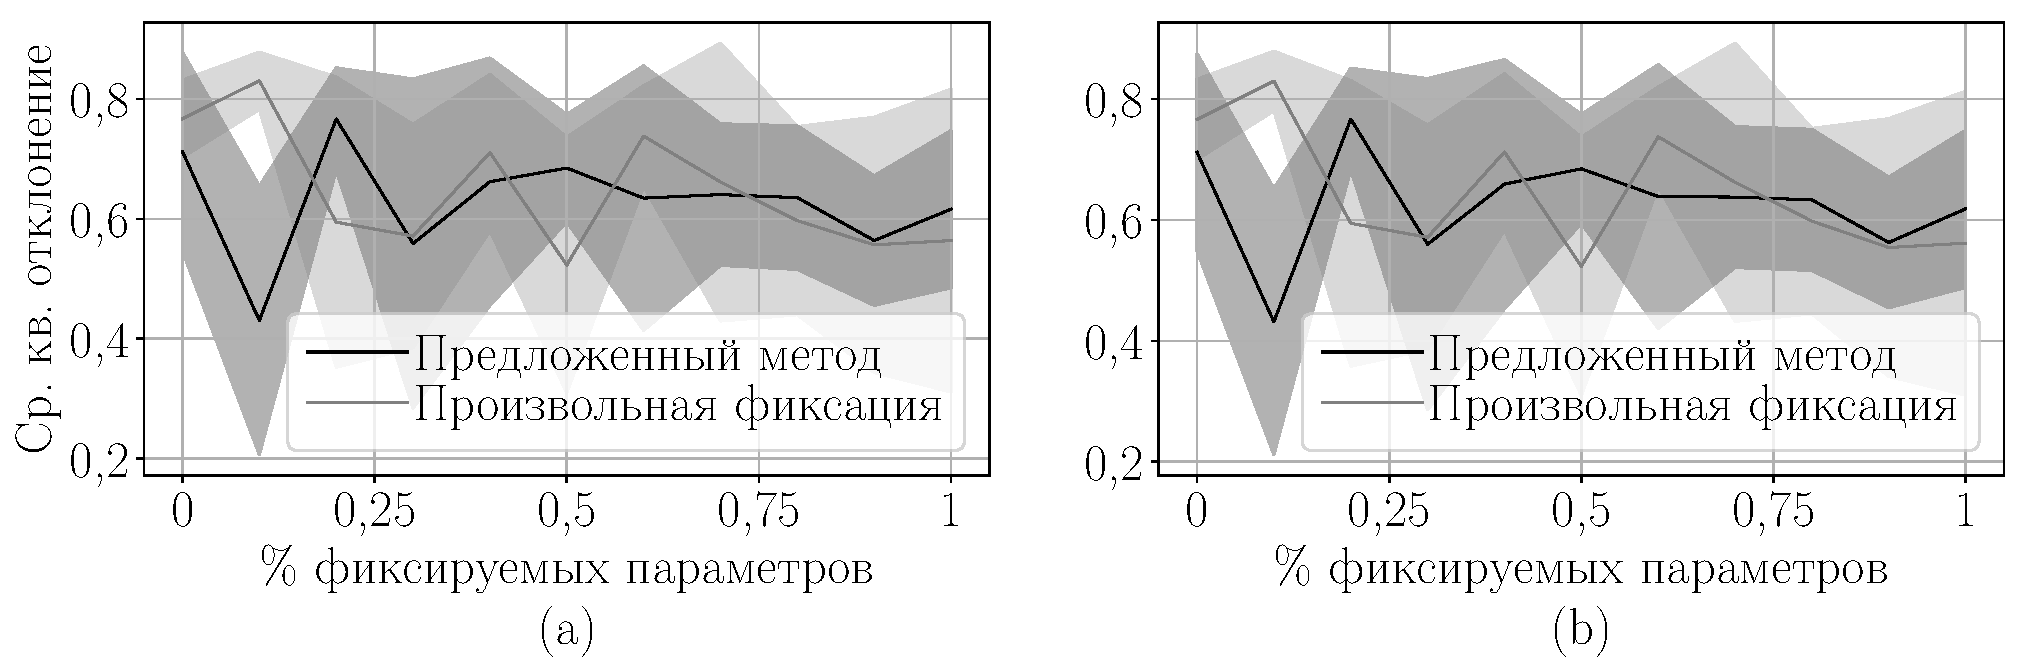
\includegraphics[width=1\textwidth]{results/order/mnist_data_loss}
\caption{Зависимость качества модели от числа зафиксированных параметров: a) на обучающей выборке; b) на тестовой выборке}
\label{fg:ex:mnist:1}
\end{figure}

\begin{figure}[h!t]\center
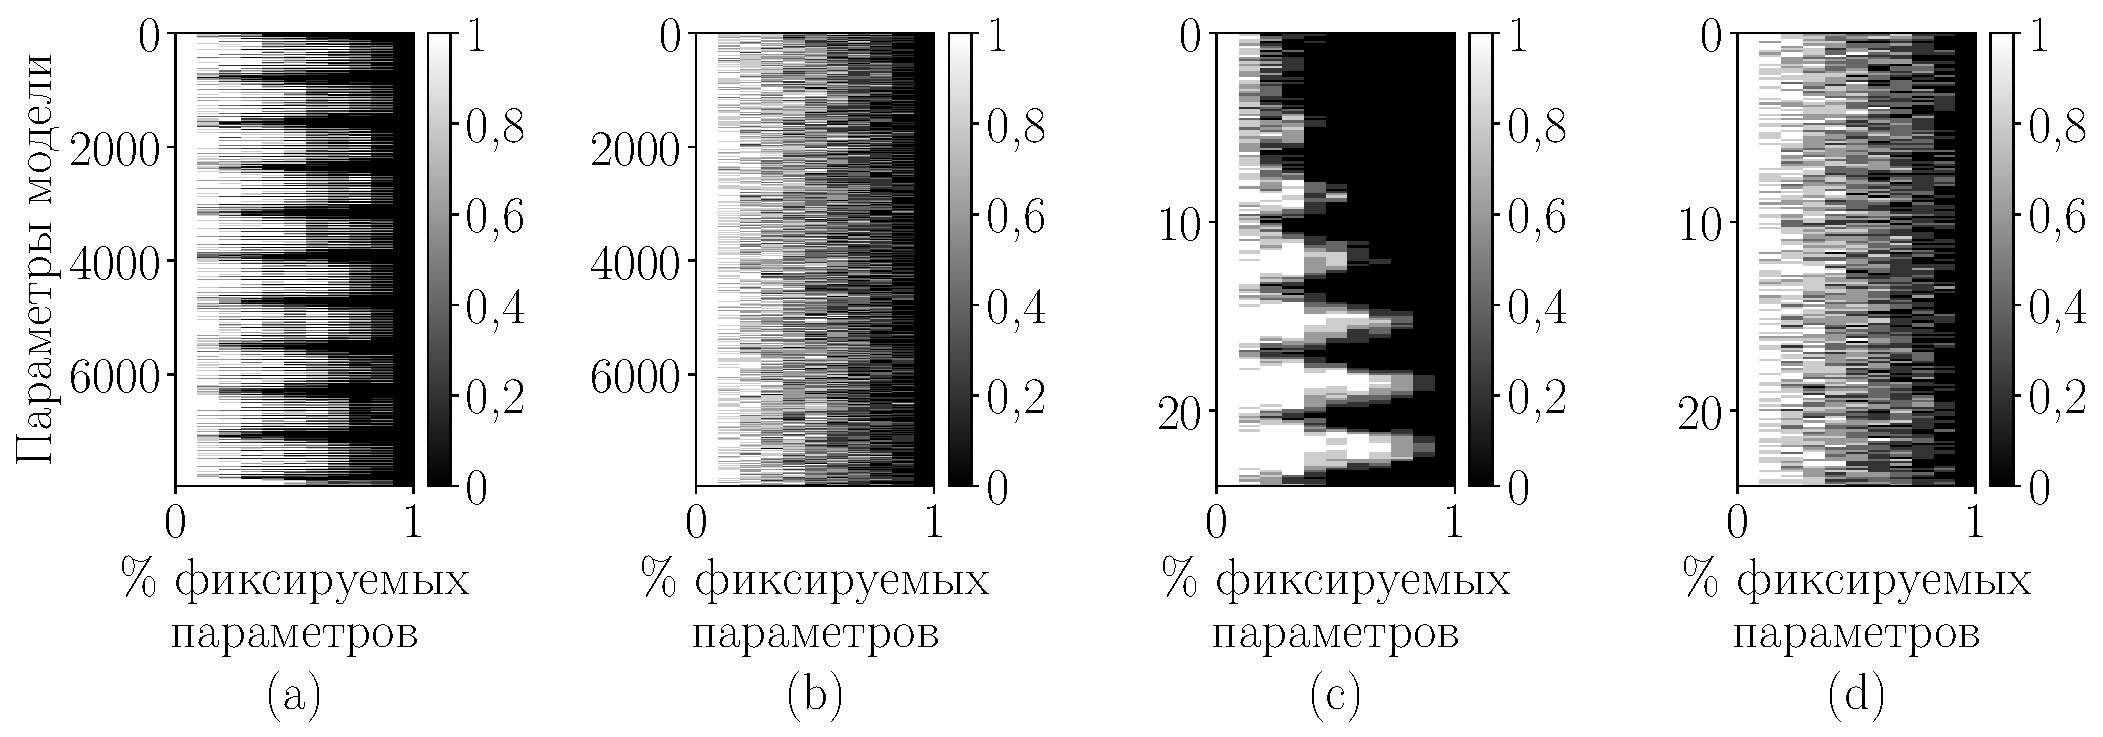
\includegraphics[width=1\textwidth]{results/order/mnist_data_matshow}
\caption{Визуализация векторов $\hat{\bm{\alpha}}\bigr(k\bigr)$ в зависимости от числа фиксируемых параметров: a) все параметры модели упорядочены предложенным методом; b) все параметры модели упорядочены произвольным образом; c) часть параметров модели упорядочена предложенным методом; d) часть параметров модели упорядочена произвольным образом}
\label{fg:ex:mnist:2}
\end{figure}

В эксперименте рассматривался двухслойный перцептрон для классификации изображений. В качестве входных данных рассматривались изображения размера $28\times28$, на которых изображены цифры. 

На рис. \ref{fg:ex:mnist:1} показано, что графики функции ошибки похожи в случае фиксации параметров параметров предложенным методом и в случае произвольной фиксации. Данный результат есть следствие того факта, что нейросеть является заведомо переусложненной моделью с большим числом параметров. После фиксации большого числа параметров у нейросети все еще остается значимое число параметров модели для дообучения.

На рис. \ref{fg:ex:mnist:2} показано, что в случае модели со значимым числом оптимизационных параметров,предложенный метод упорядочения параметров устойчив от запуску к запуску.


\newpage

\section{Релевантность параметров параметрических моделей}
Данная работа посвящена прореживанию структуры сети. Предлагается удалять наименее релевантные параметры модели. Под релевантностью~\cite{cun1990} подразумевается то, насколько параметр влияет на функцию ошибки. Малая релевантность указывает на то, что удаление этого параметра не влечет значимого изменения функции ошибки. Метод предлагает построение исходной избыточной сложности нейросети с большим количеством избыточных параметров. Для определения релевантности параметров предлагается оптимизацировать параметры и гиперпараметры в единой процедуре. Для удаления параметров предлагается использовать метод Белсли~\cite{neychev2016}.

\subsection{Постановка задачи к назначению релевантности параметрам модели}

Задана выборка
$$\mathfrak{D} = \{\textbf{x}_i,y_i\},~ i =1,...,N, \eqno(2.1)$$
где $\textbf{x}_i \in \mathbb{R}^{m}$, $y_i \in \{1, \dots, Y\}$, $Y$ --- число классов.
Рассмотрим модель $f(\mathbf{x}, \mathbf{w}): \mathbb{R}^m \times \mathbb{R}^n \to \{1,\dots,Y\}$, где $\textbf{w} \in \mathbb{R}^n$ --- пространство параметров модели,

$$f(\mathbf{x}, \mathbf{w}) = \text{softmax}\bigl( f_1(f_2(...(f_l(\mathbf{x}, \mathbf{w})\bigr), \eqno(2.2)$$
где $f_i(\mathbf{x}, \mathbf{w}) =  \text{tanh}(\mathbf{w}^\mathsf{T}\mathbf{x})$, $l$ --- число слоев нейронной сети, $i \in \{1\dots l\}$.
Параметр $w_j$ модели $f$  называется активным, если $w_j \not = 0$. Множество индексов активных параметров обозначим $\mathcal{A} \subset \mathcal{J} = \{1,...,n\}$.
Задано пространство параметров модели:
$$\mathbb{W_\mathcal{A}} = \{ \textbf{w} \in \mathbb{R}^n~|~w_j\not=0,~j \in \mathcal{A}  \}, \eqno(2.3)$$


Для модели $f$ с множеством индексов активных параметров $\mathcal{A}$ и соответствующего ей вектора параметров $\textbf{w} \in \mathbb{W_\mathcal{A}}$  определим логарифмическую функцию правдоподобия выборки:
$$\mathcal{L}_\mathfrak{D}(\mathfrak{D}, \mathcal{A}, \textbf{w}) = \log p(\mathfrak{D}|\mathcal{A}, \textbf{w}), \eqno(2.4)$$
где $p(\mathfrak{D}|\mathcal{A},\textbf{w})$ --- апостериорная вероятность выборки $\mathfrak{D}$ при заданных $\textbf{w}, \mathcal{A}$.
Оптимальные значения $\textbf{w},\mathcal{A}$ находятся из минимизации $-\mathcal{L}_{\mathcal{A}}(\mathfrak{D},\mathcal{A})$ --- логарифма правдоподобия модели:
$$\mathcal{L}_{\mathcal{A}}(\mathfrak{D},\mathcal{A}) =\log p(\mathfrak{D}|\mathcal{A}) = \log  \int_{{\textbf{w}\in\mathbb{W_\mathcal{J}}}}
p(\mathfrak{D} | \textbf{w}) p(\textbf{w} | \mathcal{A}) d \textbf{w}, \eqno(2.5)$$
где $p(\textbf{w}|\mathcal{A})$ ---  априорная вероятность вектора параметров в пространстве $\mathbb{W_\mathcal{J}}$.

Так как вычисление интеграла (2.5) является вычислительно сложной задачей, рассмотрим вариационный подход~\cite{bishop2006} для решения этой задачи. Пусть задано распределение $q$:
$$q(\textbf{w})\sim \mathcal{N}(\textbf{m}, \textbf{A}^{-1}_\text{ps}), \eqno(2.6)$$
где $\textbf{m}, \textbf{A}^{-1}_\text{ps}$ --- вектор средних и матрица ковариации, аппроксимирующее неизвестное апостериорное распределение $p(\textbf{w}|\mathfrak{D},\mathcal{A})$:
$$p(\textbf{w} | \mathcal{A})\sim \mathcal{N}(\boldsymbol{\mu},\textbf{A}^{-1}_{\text{pr}}), \eqno(2.7)$$
где $\boldsymbol{\mu},\textbf{A}^{-1}_{\text{pr}}$ --- вектор средних и матрица ковариации.

Приблизим интеграл (2.5) методом предложеном в \cite{bishop2006}:
$$\mathcal{L}_{\mathcal{A}}(\mathfrak{D},\mathcal{A}) = \log p(\mathfrak{D}|\mathcal{A}) = $$
$$ =\int_{\textbf{w}\in\mathbb{W_\mathcal{J}}} q(\textbf{w}) \log \frac{p(\mathfrak{D}, \textbf{w}|\mathcal{A})}{q(\textbf{w})}d \textbf{w} - \int_{\textbf{w}\in\mathbb{W_\mathcal{J}}}  q(\textbf{w}) \log \frac{p(\textbf{w}|\mathfrak{D},\mathcal{A})}{q(\textbf{w})}d \textbf{w} \approx $$
$$\approx \int_{\textbf{w}\in\mathbb{W_\mathcal{J}}} q(\textbf{w}) \log \frac{p(\mathfrak{D}, \textbf{w}|\mathcal{A})}{q(\textbf{w})}d \textbf{w} = $$
$$= \int_{\textbf{w}\in\mathbb{W_\mathcal{J}}} q(\textbf{w}) \log \frac{p(\textbf{w}| \mathcal{A})}{q(\textbf{w})}d \textbf{w} + \int_{\textbf{w}\in\mathbb{W_\mathcal{J}}} q(\textbf{w}) \log p(\mathfrak{D}|\mathcal{A}, \textbf{w})d \textbf{w}=$$

$$=\mathcal{L}_\textbf{w}(\mathfrak{D}, \mathcal{A}, \textbf{w})+\mathcal{L}_{E}(\mathfrak{D},\mathcal{A}). \eqno(2.8)$$

Первое слагаемое формулы (2.8) --- это сложность модели. Оно определяется расстоянием Кульбака-Лейблера:
$$\mathcal{L}_\textbf{w}(\mathfrak{D}, \mathcal{A}, \textbf{w}) = -D_{KL}\bigl(q(\textbf{w})||p(\textbf{w}|\mathcal{A})\bigr). \eqno(2.9)$$
Второе слагаемое формулы (2.8) является матожиданием правдоподобия выборки $\mathcal{L}_\mathfrak{D}(\mathfrak{D},\mathcal{A}, \textbf{w})$. В данной работе оно является функцией ошибки:
$$\mathcal{L}_{E}(\mathfrak{D},\mathcal{A}) = \mathsf{E}_{\textbf{w}\sim q}\mathcal{L}_\mathfrak{D}(\textbf{y}, \mathfrak{D}, \mathcal{A}, \textbf{w}). \eqno(2.10)$$

Требуется найти параметры, доcтавляющие минимум суммарному функционалу потерь $\mathcal{L}_\mathcal{A}(\mathfrak{D},\mathcal{A},\textbf{w})$ из (2.8):
$$\hat{\textbf{w}} = \argmin_{\mathcal{A}\subset\mathcal{J},~\textbf{w} \in \mathbb{W_\mathcal{A}}} -\mathcal{L}_\mathcal{A}(\mathfrak{D}, \mathcal{A}, \textbf{w}) = $$
$$=\argmin_{\mathcal{A}\subset\mathcal{J},~\textbf{w} \in \mathbb{W_\mathcal{A}}} D_{KL}\bigl(q(\textbf{w})||p(\textbf{w}|\mathcal{A})\bigr) - \mathcal{L}_\mathfrak{D}(\mathfrak{D}, \mathcal{A}, \textbf{w}). \eqno(2.11)$$

\paragraph{Случайное удаление.}
Метод случайного удаления заключается в том, что случайным образом удаляется некоторый параметр $w_\xi$ из множества активных параметров сети.  Индекс параметра $\xi$ из равномерного распределения  случайная величина, предположительно доставляющая оптимум в (2.11).
$$\xi \sim \mathcal{U}(\mathcal{A}). \eqno(3.1.1)$$

\paragraph{Оптимальное прореживание.}
Метод оптимального прореживания \cite{cun1990} использует вторую производную целевой функции (2.4) по параметрам для определения нерелевантных параметров. Рассмотрим функцию потерь $\mathcal{L}$ (2.4) разложенную в ряд Тейлора в некоторой окрестности вектора параметров $\textbf{w}$:
$$\delta \mathcal{L} = \sum_{j\in \mathcal{A}} g_j\delta w_j + \frac{1}{2}\sum_{i,j\in \mathcal{A}} h_{ij}\delta w_i\delta w_j + O(||\delta\textbf{w}||^3), \eqno(3.2.1)$$
где $\delta w_j $ --- компоненты вектора $\delta\textbf{w}$, $g_j$ --- компоненты вектора градиента $\nabla \mathcal{L}$, а $h_{ij}$ --- компоненты гесcиана $\textbf{H}$:
$$g_j = \frac{\partial \mathcal{L}}{\partial w_j}, \qquad h_{ij} = \frac{\partial^2\mathcal{L}}{\partial w_i \partial w_j}. \eqno(3.2.2)$$

Задача является вычислительно сложной в силу размерности матрицы \textbf{H}. Введем следующее предположение \cite{cun1990}, о том что удаление нескольких параметров приводит к такому же изменению функции потерь $\mathcal{L}$, как и суммарное изменение при индивидуальном удалении:
$$\delta \mathcal{L} = \sum_{j\in \mathcal{A}} \delta \mathcal{L}_j, \eqno(3.2.3)$$
где $\mathcal{A}$ --- множество активных параметров, $\delta\mathcal{L}_j$ --- изменение функции потерь, при удалении одного параметра $\textbf{w}_j$.

В силу данного предположения будем рассматривать только диагональные элементы матрицы \textbf{H}. После введенного предположения, выражение (3.2.1) принимает вид
$$\delta \mathcal{L} = \frac{1}{2} \sum_{j\in \mathcal{A}} h_{jj}\delta w_j^2, \eqno(3.2.4)$$

Получаем следующую задачу оптимизации:

$$\xi = \argmin_{j\in \mathcal{A}} h_{jj}\frac{w_j^2}{2}, \eqno(3.2.5)$$
где $\xi$ --- индекс наименее релевантного, удаляемого параметра, предположительно доставляющая оптимум в (2.11).

\paragraph{Удаление неинформативных параметров с помощью вариационного вывода.}
Для удаления параметров в работе \cite{graves2011} предлагается удалить параметры, которые имеют максимальное отношение плотности $p(\textbf{w}|\mathcal{A})$ априорной вероятности в нуле к плотности вероятности априорной вероятности в математическом ожидании параметра.\\
Для гауссовского распределения с диагональной матрицей ковариации получаем:
$$p_j(\textbf{w}|\mathcal{A})(x) = \frac{1}{\sqrt[]{2\sigma_j^2}}\exp({-\frac{(x-\mu_j)^2}{2\sigma_j^2}}). \eqno(3.3.1)$$
Разделив плотность вероятности в нуле к плотности в математическом ожидание
$$ \frac{p_j(\textbf{w}|\mathcal{A})(0)}{p_j(\textbf{w}|\mathcal{A})(\mu_j)}= \exp({-\frac{\mu_j^2}{2\sigma_j^2}}), \eqno(3.3.2)$$
Получаем следующую задачу оптимизации:
$$\xi = \argmin_{j\in \mathcal{A}} \left|\frac{\mu_j}{\sigma_j}\right|, \eqno(3.3.3)$$
где $\xi$ --- индекс наименее релевантного, удаляемого параметра.

\paragraph{Прореживание сети на основе метода Белсли.}
Предлагается метод основанный на модификации метода Белсли. Пусть $\textbf{w}$ --- вектор параметров доставляющий минимум функционалу потерь $\mathcal{L}$ на  множестве $\mathbb{W_\mathcal{A}}$, а $\textbf{A}_\text{ps}$ соответствующая ему ковариационная матрица.

Выполним сингулярное разложение матрицы
$$\textbf{A}_\text{ps} = \textbf{U}{\bf\Lambda}\textbf{V}^\mathsf{T}. \eqno(4.1)$$
Индекс обусловленности $\eta_{j}$ определим как отношение максимального элемента к $j$-му элементу матрицы ${\bf\Lambda}$. Для нахождения мультиколлиниарных признаков требуется найти индекс $\xi$ вида:
$$\xi = \argmax_{j\in \mathcal{A}}{\eta_j}. \eqno(4.2)$$

\begin{figure}[h!t]\center
\subfloat[Матрица ковариации]{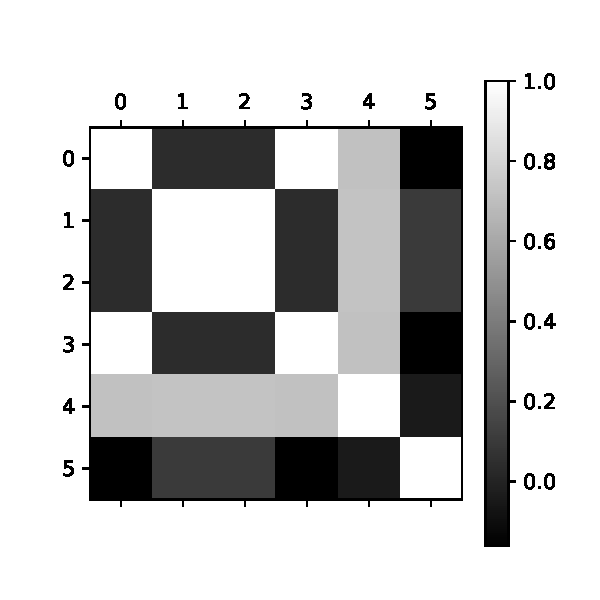
\includegraphics[width=0.5\textwidth]{results/relevant/Cov.pdf}}
\subfloat[Дисперсионные доли]{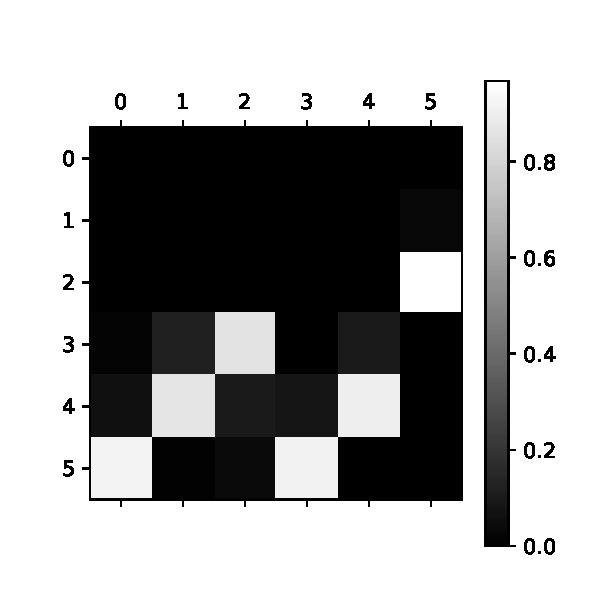
\includegraphics[width=0.5\textwidth]{results/relevant/BelslyImage.pdf}}
\caption{Илюстрация метода Белсли}
\label{CovBel}
\end{figure}

\begin{table}[h]
\begin{center}
\caption{Илюстрация метода Белсли}
\begin{tabular}{|c|cccccc|}
\hline
$\eta$ & $q_1$& $q_2$& $q_3$& $q_4$& $q_5$& $q_6$\\
\hline
$1.0$ &  $2\cdot 10^{-17}$ &  $4\cdot 10^{-17}$ &  $1\cdot 10^{-16}$ &  $2\cdot 10^{-17}$ &  $6\cdot 10^{-17}$&  $3\cdot 10^{-4}$ \\
\hline
$1.5$ &  $5\cdot 10^{-17}$ &  $9\cdot 10^{-17}$ &  $2\cdot 10^{-16}$ &  $5\cdot 10^{-17}$ &  $3\cdot 10^{-20}$ &  $3\cdot 10^{-2}$ \\
\hline
$3.3$ &  $9\cdot 10^{-18}$ &  $1\cdot 10^{-17}$ &  $2\cdot 10^{-17}$ &  $9\cdot 10^{-18}$ &  $2\cdot 10^{-19}$ &  $9\cdot 10^{-1}$ \\
\hline
$2\cdot 10^{15}$ &  $1\cdot 10^{-2}$ &  $1\cdot 10^{-1}$ &  $8\cdot 10^{-1}$ &  $2\cdot 10^{-3}$ &  $9\cdot 10^{-2}$ &  $1\cdot 10^{17}$ \\ 
\hline
$8\cdot 10^{15}$ &  $6\cdot 10^{-2}$ &  $8\cdot 10^{-1}$ &  $9\cdot 10^{-2}$ &  $8\cdot 10^{-2}$ &  $9\cdot 10^{-1}$ & $ 2\cdot 10^{17} $\\
\hline
$1\cdot 10^{16}$ &  $\bf9\cdot 10^{-1}$ &  $1\cdot 10^{-2}$& $ 4\cdot 10^{-2}$&  $\bf9\cdot 10^{-1}$ &  $1\cdot 10^{-3}$ & $ 5\cdot 10^{-21}$ \\
\hline
\end{tabular}
\label{CovBelTable}
\end{center}
\end{table}

Дисперсионный долевой коэффициент $q_{ij}$ определим как вклад $j$-го признака в дисперсию $i$-го элемента вектора параметра $\textbf{w}$:

$$q_{ij} = \frac{u^2_{ij}/\lambda_{jj}}{\sum^n_{j=1}{u^2_{ij}/\lambda_{jj}}}. \eqno(4.3)$$

Большие значение дисперсионных долей указывают на наличие зависимости между параметрами. Находим долевые коэффициенты, которые вносят максимальный вклад в дисперсию параметра $w_\xi$:

$$\zeta = \argmax_{j\in \mathcal{A}}{q_{\xi j}}. \eqno(4.4)$$
Параметр с индексом $\zeta$ определим как наименее релевантный параметр нейросети. 
%Для удаления нескольких зависимых параметров за раз, предлагается удалить параметры с номерами $p \in \mathcal{A}: q_{\xi i} > \lambda  \in  \mathbb{R}_+$.

Проиллюстрируем принцип работы метода Белсли на примере. Рассмотрим данные порожденные следующим образом: 
$$\textbf{w} = \begin{bmatrix}
\text{sin}(x)\\
\text{cos}(x)\\
\text{2+cos}(x)\\
\text{2+sin}(x)\\
\text{cos}(x) + \text{sin}(x)\\
x
\end{bmatrix}$$
с матрицей ковариации на рис.~\ref{CovBel}.a, где $x \in [0.0, 0.02, ..., 20.0]$.


В табл.~\ref{CovBelTable} приведены индексы обусловленности и соответствующие им дисперсионные доли, которые также изображены на рис.~\ref{CovBel}.b. Согласно этим данным, максимальный индекс обусловленности $\eta_6 = 1.2\cdot 10^{16}$. Ему соответствуют максимальные дисперсионные доли признаков с индексами 1 и 4, которые, как видно из построения выборки, являются линейно зависимые.

\subsection{Анализ разных подходов к определению релевантности}
Для анализа свойств предложенного алгоритма и сравнения его с существующими был проведен вычислительный эксперимент в котором параметры нейросети удалялись методами,  которые были описаны в разделах 3.1---3.3 и методом Белсли.

В качестве данных использовались три выборки. Выборки Wine \cite{Wine} и Boston Housing \cite{Boston}  --- это реальные данные. Синтетические данные сгенерированы таким образом чтобы параметры сети были мультиколинеарными. Генерация данных состояла из двух этапов. 
На первом этапе генерировался вектор параметров $\mathbf{w}_{\text{synthetic}}$:
$$\mathbf{w}_{\text{synthetic}}  \sim \mathcal{N}(\textbf{m}_{\text{synthetic}}, \textbf{A}_{\text{synthetic}}), \eqno(5.1)$$ 
где 
$\textbf{m}_{\text{synthetic}} = \begin{bmatrix}
1.0\\
0.0025\\
\cdots\\
0.0025
\end{bmatrix}$,
$\textbf{A}_{\text{synthetic}} = \begin{bmatrix}
1.0& 10^{-3}& \cdots& 10^{-3}& 10^{-3}\\
10^{-3}& 1.0& \cdots& 0.95& 0.95\\
\cdots&\cdots&\cdots&\cdots&\cdots\\
10^{-3}& 0.95& \cdots& 0.95& 1.0
\end{bmatrix}$.

На втором этапе генерировалась выборка $\mathfrak{D}_{\text{synthetic}}$:
$$\mathfrak{D}_{\text{synthetic}} = \{(\textbf{x}_i,y_i)| \textbf{x}_i \sim  \mathcal{N}(\textbf{1}, \textbf{I}), y_i = x_{i0}, i = 1 \cdots 10000\}. \eqno(5.2)$$
В приведенном выше векторе параметров $\mathbf{w}_{\text{synthetic}}$ для выборки $\mathfrak{D}_{\text{synthetic}}$, наиболее релевантным является первый параметр, а все остальные параметры являются нерелевантными. Матрица ковариации была выбрана таким образом, чтобы все нерелевантные параметры были зависимы и метод Белсли был максимально эффективен.



\begin{table}[h]

\begin{center}
\caption{Описание выборок}
\begin{tabular}{|c|c|c|c|}
\hline
	Выборка &Тип задачи& Размер выборки& Число признаков\\
	\hline
	
	\multicolumn{1}{|l|}{Wine}
	&
	\multicolumn{1}{|l|}{класификация}
	 & 178 & 13\\
	\hline
	
	\multicolumn{1}{|l|}{Boston Housing}
	&
	\multicolumn{1}{|l|}{регресия}
	& 506 & 13\\
	\hline
	
	\multicolumn{1}{|l|}{Synthetic data}
	&
	\multicolumn{1}{|l|}{регресия}
	& 10000 & 100\\
\hline

\end{tabular}
\end{center}
\end{table}



Для алгоритмов тренировочная и тестовая выборки составили $80\%$ и $20\%$ соответсвенно. Критерием качества прореживания служит процент параметров нейросети, удаление которого не влечет значимой потери качества прогноза. Также критерием качества служит устойчивость нейросети к зашумленности данных. 

Качеством прогноза $R_{\text{cl}}$ модели для задачи классификации является точность прогноза модели:
$$R_{\text{cl}} = \frac{\sum_{(\textbf{x},y)\in \mathfrak{D}} [f(\textbf{x}, \textbf{w}) = y]}{\left|\mathfrak{D}\right|}, \eqno(5.3)$$

Качеством прогноза $R_{\text{rg}} $ модели для задачи регрессии является среднеквадратическое отклонение результата модели от точного:

$$R_{\text{rg}} = \frac{\sum_{(\textbf{x},y)\in \mathfrak{D}} \left(f(\textbf{x}, \textbf{w}) - y\right)^2}{\left|\mathfrak{D}\right|}, \eqno(5.4)$$

\paragraph{Wine.} Рассмотрим нейроную сеть с 13 нейронами на входе, 13 нейронами в скрытом слое и 3 нейронами на выходе.

\begin{figure}[h!t]\center
\includegraphics[width=0.8\textwidth]{results/relevant/WIne/All.pdf}\\
\caption{Качество прогноза при удаление параметров на выборке Wine}
\label{WineAll}
\end{figure}

\begin{figure}[h!t]\center
\subfloat[Произвольное удаление параметров]{\includegraphics[width=0.5\textwidth]{results/relevant/WIne/RandomNoise3D.pdf}}
\subfloat[Оптимальное прореживание]{\includegraphics[width=0.5\textwidth]{results/relevant/WIne/OBDNoise3D.pdf}}\\
\subfloat[Вариационный метод]{\includegraphics[width=0.5\textwidth]{results/relevant/WIne/VariationalNoise3D.pdf}}
\caption{Влияние шума в начальных данных на шум выхода нейросети на выборке Wine}
\label{WineNoise}
\end{figure}

На рис.~\ref{WineAll} показано как меняется точность прогноза $R_{\text{cl}}$ при удалении параметров указанными методами. Из графика видно, что метод оптимального прореживания, вариационный метод и метод Белсли позволяют удалить $\approx80\%$ параметров и качество всех этих методов падает при удалении $\approx90\%$ параметров нейросети. 

На рис.~\ref{WineNoise} показаны поверхности изменения уровня шума ответов нейросети при изменении процента удаленных параметров и уровня шума входных данных для разных методов прореживания. На графиках показано, что при удалении параметров нейросети методом Белсли шум меньше, чем при удалении параметров другими методами, на это указывает то что поверхность которая соответствует методу Белсли ниже других поверхностей.

\paragraph{Boston Housing.} Рассмотрим нейроную сеть с 13 нейронами на входе, 39 нейронами в скрытом слое и одним нейроном на выходе.

\begin{figure}[h!t]\center
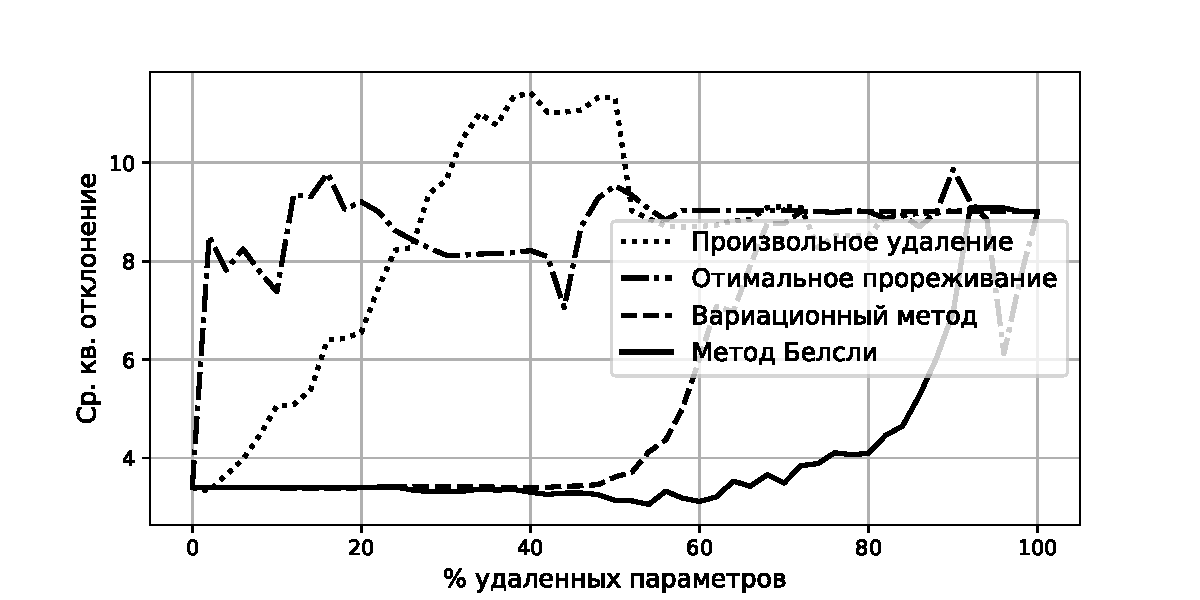
\includegraphics[width=0.8\textwidth]{results/relevant/Boston/All.pdf}\\
\caption{Качество прогноза при удаление параметров на выборке Boston}
\label{BostonAll}
\end{figure}

\begin{figure}[h!t]\center
\subfloat[Произвольное удаление параметров]{\includegraphics[width=0.5\textwidth]{results/relevant/Boston/RandomNoise3D.pdf}}
\subfloat[Оптимальное прореживание]{\includegraphics[width=0.5\textwidth]{results/relevant/Boston/OBDNoise3D.pdf}}\\
\subfloat[Вариационный метод]{\includegraphics[width=0.5\textwidth]{results/relevant/Boston/VariationalNoise3D.pdf}}
\caption{Влияние шума в начальных данных на шум выхода нейросети на выборке Boston}
\label{BostonNoise}
\end{figure}

На рис.~\ref{BostonAll} показано как меняется среднеквадратическое отклонение прогноза $\mathsf{R}_{\text{rg}}$ от точного ответа  при удалении параметров указанными методами. График показывает, что метод Белсли является более эффективным, чем другие методы, так-как позволяет удалить больше параметров нейросети без потери качества.

На рис.~\ref{BostonNoise} показаны поверхности изменения уровня шума ответов нейросети при изменении процента удаленных параметров и уровня шума входных данных для разных методов прореживания. График показывает, что уровень шума всех методов одинаковый, так-как поверхности всех методов находятся на одном уровне.


\paragraph{Синтетические данные.} Рассмотрим нейроную сеть с 100 нейронами на входе и одним нейроном на выходе.

\begin{figure}[h!t]\center
\includegraphics[width=0.8\textwidth]{results/relevant/Data1/All.pdf}\\
\caption{Качество прогноза при удаление параметров на синтетической выборке}
\label{Data1All}
\end{figure}

\begin{figure}[h!t]\center
\subfloat[Произвольное удаление параметров]{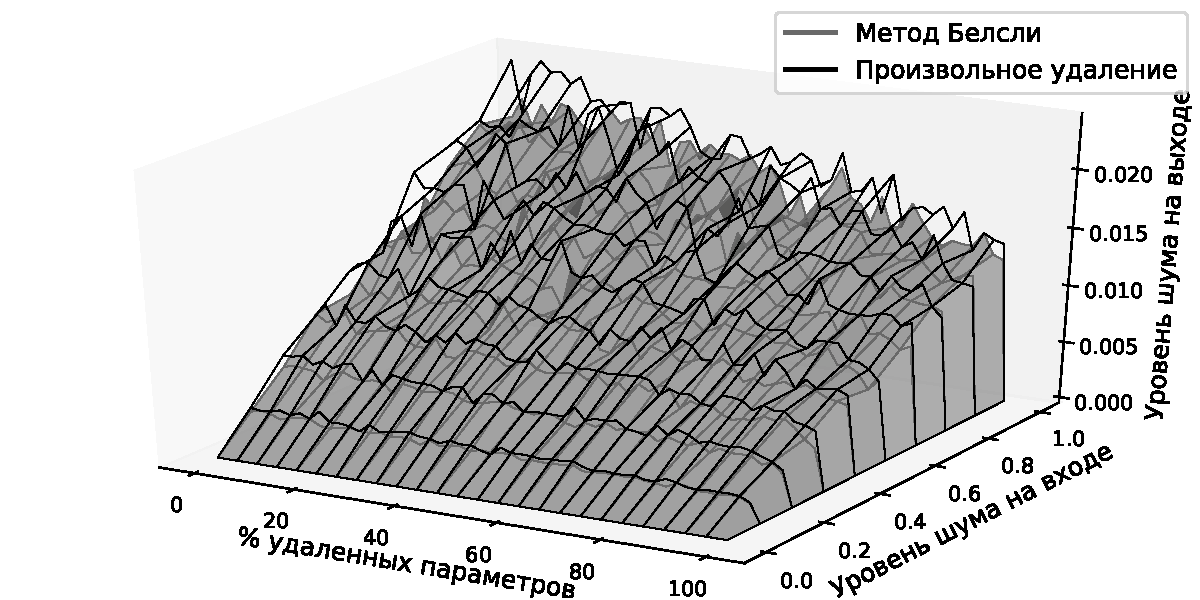
\includegraphics[width=0.5\textwidth]{results/relevant/Data1/RandomNoise3D.pdf}}
\subfloat[Оптимальное прореживание]{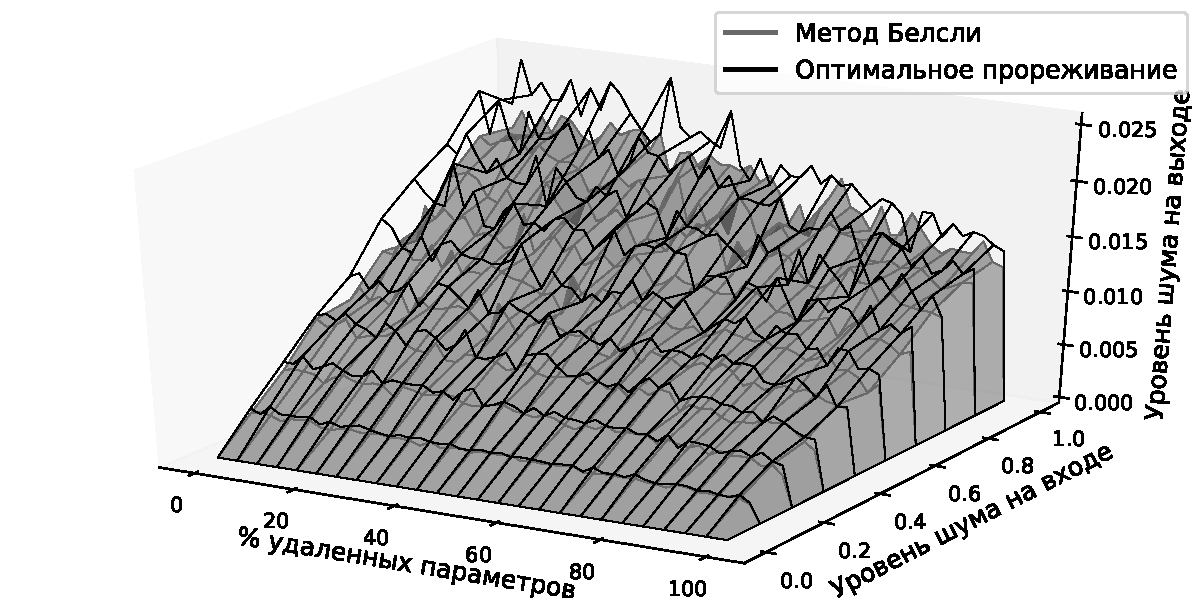
\includegraphics[width=0.5\textwidth]{results/relevant/Data1/OBDNoise3D.pdf}}\\
\subfloat[Вариационный метод]{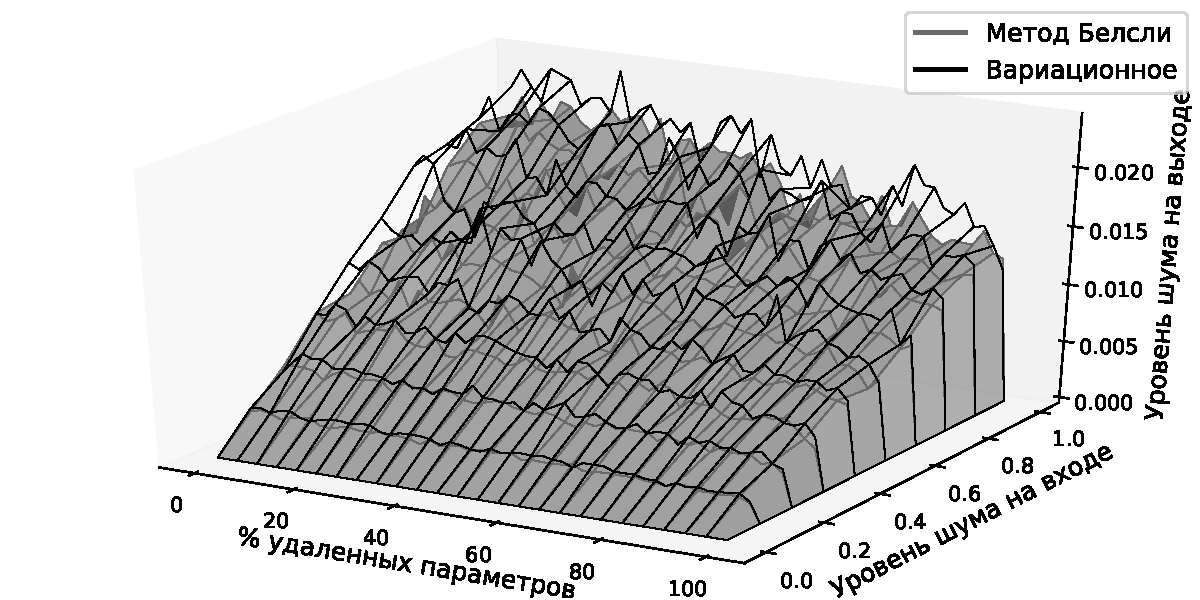
\includegraphics[width=0.5\textwidth]{results/relevant/Data1/VariationalNoise3D.pdf}}
\caption{Влияние шума в начальных данных на шум выхода нейросети на синтетической выборке}
\label{Data1Noise}
\end{figure}

На рис.~\ref{Data1All} показано как меняется среднеквадратическое отклонение прогноза от $\mathsf{R}_{\text{rg}}$ точного ответа при удалении параметров указанными методами. График показывает, что удаление параметров методом Белсли являеться более эффективным чем другие методы прореживания, так-как качество прогноза нейросети улучшается при удалении шумовых параметров.

На рис.~\ref{Data1Noise} показаны поверхности изменения уровня шума ответов нейросети при изменении процента удаленных параметров и уровня шума входных данных для разных методов прореживания. На графиках показано, что при удалении параметров нейросети методом Белсли шум меньше, чем при удалении параметров другими методами, так-как поверхность которая соответствует методу Белсли ниже других поверхностей.

\newpage

\section{Определения оптимального размера выборки для линейных моделей}
\subsection{Описание задачи}
The design of experiment requires to estimate the minimum sample size: the quantity of the performed feature set measurements which are required to build the formulated conditions. The choice of the sample size estimation method depends on the problem being solved which determines the formulation of the statistical hypothesis and statistics to check it. Table~\ref{table1} presents ten sample size estimation methods. It includes both classical and Bayesian methods of the sample size estimation.

The classical methods assume that the sample corresponds to some prior conditions formulated earlier. These conditions are formulated as a statistical criterion~(Self et al. 1988, 1992; Shieh 2000; Demidenko 2007). The sample size estimation method related to this criterion guarantees that the fixed statistical power $1-\beta$ with the extent of the first kind error which does not exceed the set value $\alpha$ will be approached. This sample size is called sufficient.

\begin{table}
\begin{center}
\caption{Methods}
\label{table1}
\begin{tabular}{|p{0.15\textwidth}|p{0.6\textwidth}|p{0.15\textwidth}|}
\hline
	\centering Method &\centering Short overview & Reference\\
\hline
	Lagrange multipliers test &
	Likelihood of the sample has the following form:
   	$p(y|\textbf{x}, \textbf{w}) = \exp\bigl(y\theta- b(\theta) + c\left(y\right)\bigr).$
	Sufficient sample size $m^*$:
	$m^* = \frac{\gamma^*}{\gamma^0}$, where $\gamma^*$ and $\gamma_0$ can be found in \eqref{eq:sb:6} and \eqref{eq:sb:5}.
	&Self et al. 1988\\
\hline
	Likelihood ratio test&
	Likelihood of the sample has the following form:
	$p(y|\textbf{x}, \textbf{w}) = \exp\left(\frac{y\theta- b(\theta)}{a(\phi)} + c\left(y, \phi\right)\right).$
	Sufficient sample size $m^*$: 
	$m^* = \frac{\gamma^*}{\Delta^*},$ where $\gamma^*$ and $\Delta^*$ can be found from \eqref{eq:sb:11} and \eqref{eq:sb:13}.
	&Shieh 2000\\
\hline
	Wald statistic&
	Likelihood of the sample has the following form:
	$p(y|\textbf{x}, \textbf{w}) = \exp\left(\frac{y\theta- b(\theta)}{a(\phi)} + c\left(y, \phi\right)\right).$
	
	Sufficient sample size $m^*$: 
	
	$m^* = \frac{\gamma^*}{\delta},$ where$\gamma^*$ and $\delta$ can be found from \eqref{eq:sb:20}.
	&Shieh 2005\\
\hline
	Cross-validation&
	
	Sufficient sample size $m^*$: 
	
	$~\forall m \geq m^*~RS(m) \geq 1- \varepsilon,$
	where~$\varepsilon$ is chosen such that, $RS$ is defined in~\eqref{eq:hb:5}.
	&Motrenko et al. 2014\\
\hline
	Bootstrap&
	
	Sufficient sample size  $m^*: \forall m\geq m^* \max_i\left(b^m_i - a^m_i\right) < l$, where $(a^m_i,  b^m_i)$ is quantile bootstrap confident interval calculated on $i$-th bootstrap subsample of size $m$

	&(Qumsiyeh 2013)\\
\hline
	Kullback-Leibler&
	
	Sufficient sample size $m^*$: 
	
	$\forall \mathfrak{D}_{\mathcal{B}_1}:~\left|\mathfrak{D}_{\mathcal{B}_1}\right| \geq m^*  ~ \mathsf{E}_{\mathfrak{D}_{\mathcal{B}_2}}D_\text{KL}\left(p_1, p_2\right) \leq \varepsilon,$
	where $\mathcal{B}_1,~\mathcal{B}_2$ satisfy~\eqref{eq:bs:8}.
	&Motrenko et al. 2014\\
\hline
	Average posterior variance criterion&
	
	Sufficient sample size $m^*$: 
	
	$\forall m \geq m^*  ~ \mathsf{E}_{\mathfrak{D}_m}\mathsf{D}\left[\hat{\textbf{w}}|\mathfrak{D}_m\right] \leq \varepsilon,$ where $\varepsilon$ is sufficiently small.
	&Joseph et al. 1997, 1995\\
\hline
	Average coverage criterion&
	Sufficient sample size $m^*$:
	
	$\forall m \geq m^*  ~ \mathsf{E}_{\mathfrak{D}_m}\mathsf{P}\left\{\textbf{w} \in A\left(\mathfrak{D}_m\right)\right\} \geq 1-\alpha$, where $\alpha$ is sufficiently small.
	&Joseph et al. 1997, 1995\\
\hline
	Average length criterion&
	Sufficient sample size $m^*$:
	
	$\forall m \geq m^*  ~ \mathsf{E}_{\mathfrak{D}_m}r_m\leq l,$ 
	where $r_m$ is described in \eqref{eq:bs:5}
	&Joseph et al. 1997, 1995\\
\hline
	Utility maximization&
	Sufficient sample size $m^*$:
	
	$m^* = \argmax_{m} \mathsf{E}_{\mathfrak{D}_m}\int_{\textbf{w}}u\left(\mathfrak{D}, \textbf{w}\right)p(\textbf{w}|\mathfrak{D})d\textbf{w},$
	where utility function $u\left(\mathfrak{D}, \textbf{w}\right)$ is given as \eqref{eq:bs:7}.
	&Lindley 1997\\


\hline
\end{tabular}
\end{center}
\end{table}

However, the practical applications of the sample size estimation methods assume a model to fit the measured data~(Kloek 1975). These models are selected according to either regression or classification problem statement. In this paper generalised linear models are  In the paper~(Self et al. 1988), a method of power estimation of the Lagrange multiplier test for coefficients of the generalised linear regression, with the help of which the sample size is estimated, is described. The weakness of the method is in the fact that when an alternative hypothesis differs greatly from the null hypothesis, the maximum likelihood estimates for the model parameters and covariance matrix used for power rating are not asymptotically consistent in the alternative hypothesis. Later~(Self et al. 1992) an approach to the estimation of power and sample size related to it was proposed on the basis of the maximum likelihood ratio test. This approach appeared to be more accurate for a series of independent variables. Besides, a power estimation method for Wald statistics was proposed in the paper~(Shieh 2005). In the paper~(Motrenko et al. 2014) in case of logistic regression, it is proposed that the method which uses the ROC-AUC curve and shift concept be used. The classical methods~(Self et al. 1988, 1992; Shieh 2000, 2005; Demidenko 2007) have a series of restrictions related to practical application of these methods. In order to estimate the sample size, it is required to know the parameter estimation variance or, in a more general case, to have the estimation of the non-centrality parameter in the distribution of the statistics used when the alternative hypothesis is true. These methods do not show how to obtain these values. Besides, the estimation variance and non-centrality parameter will not be obtained with a certain variance the influence of which on the sample size estimation result is irrelevant. 

Statistical methods make it possible to estimate the sample size on the basis of assumptions about the distribution of data and information about the correspondence between the values observed and the assumptions of the null hypothesis. When the size of the sample under investigation is sufficient or excessive, it is possible to use the methods based on the observation of alteration of certain characteristic of the model building procedure when enhancing the sample size. In particular, when observing the relation of the forecasting quality with the control sample and training sample~(Motrenko et al. 2014), we shall determine the sufficient sample size which corresponds to the start of over-training. In the paper~(Qumsiyeh 2013), a bootstrap method is used to estimate the sufficient sample size. The excess of the current sample size is checked on the basis of a confident intervals analysis of the parameter estimated. The width of the confident interval with different values of the sample size is estimated with the help of a bootstrap method. For this purpose, the samples of smaller size are sampled the specified number of times, and the confident interval for an error when estimating the model parameter is calculated. The sample size is considered sufficient when the width of the confident interval does not exceed a certain value set in advance.

The restrictions of statistical methods of sample size estimation listed above are considered in details in Bayesian procedure~(Lindley 1997; Rubin et al. 1998; Wang et al. 2002) where the sample size estimation is determined on the basis of maximisation of the expected merit function~(Lindley 1997). The merit function may include the explicit parameter distribution functions and penalties for the sample size enhancement. The alternative to the approaches~(Wang et al. 2002) based on the merit function is the sampling of the sample size by setting restrictions on a certain model parameter estimation quality criterion. The examples of such criteria are the following: average  posterior variance criterion (AVPC), average length criterion (ALC), average coverage criterion (ACC). For every criterion listed, the sample size estimation is determined as a minimum value of the sample size for which the expected value of the criterion chosen does not exceed any fixed threshold. In the paper~(Motrenko et al. 2014), it is proposed that the sample size be considered sufficient  if the space between the distributions estimated on the basis of subsamples of this size is sufficiently small. Such approach does not require any further generalisation in case of multiple variables. Besides, estimation may be made in the presence of data distribution assumptions, as well as in their absence. The weakness of this approach is in the fact that quantitative estimation can be obtained only when the sample size is excessive. 

\subsection{Постановка задачи определения размера выборки}

Given a sample set of size $m$:
\begin{equation}
\label{eq:ps:1}
\begin{aligned}
	\mathfrak{D}_{m} = \{\textbf{x}_i, y_i\}_{i = 1}^{m}
\end{aligned}
\end{equation}
where $\textbf{x}_i\in \mathbb{R}^{n}$, $y_i\in \mathbb{Y}$. Feature vector $\textbf{x} = [\textbf{u}, \textbf{v}]$ concatenates $\textbf{u}_i\in \mathbb{R}^{k}$ and $~\textbf{v}_i\in \mathbb{R}^{n-k}$.
The sample set $\mathfrak{D}_{m}$ randomly splits into train and test parts
\begin{equation}
\label{eq:ps:2}
\begin{aligned}
	\mathfrak{D}_{\mathcal{T}_{m}} = \{\textbf{x}_i, \textbf{y}_i\}_{i \in \mathcal{T}_{m}}, \quad \mathfrak{D}_{\mathcal{L}_{m}} = \{\textbf{x}_i, \textbf{y}_i\}_{i \in \mathcal{L}_{m}}, \quad  \mathcal{T}_{m}\sqcup\mathcal{L}_{m} = \{1, ..., m\}.
\end{aligned}
\end{equation}
Let introduce a parametric family of functions for unknown distribution approximation $p(y|\textbf{x}, \mathfrak{D}_{\mathcal{L}_{m}})$:
\begin{equation}
\label{eq:ps:3}
\begin{aligned}
	\mathfrak{F} = \left\{f\left(y,\textbf{x}, \textbf{w}\right)|\textbf{w}\in\mathbb{W},~\int_{y\in \mathbb{Y}, \textbf{x}\in\mathbb{R}^{n}}f\left(y, \textbf{x}, \textbf{w}\right)dyd\textbf{x}=1\right\}.
\end{aligned}
\end{equation}

For the model $f$ with the parameters vector $\textbf{w}$ define the likelihood function and logarithmic likelihood function of the sample set $\mathfrak{D}$:
\begin{equation}
\label{eq:ps:4}
\begin{aligned}
	L\left(\mathfrak{D}, \textbf{w}\right) = \prod f\left(y,\textbf{x}, \textbf{w}\right),\quad l\left(\mathfrak{D}, \textbf{w}\right) = \sum \log f\left(y,\textbf{x}, \textbf{w}\right),
\end{aligned}
\end{equation}

where $f(y,\textbf{x}, \textbf{w})$ is the likelihood of the sample set $\mathfrak{D}_{\mathcal{L}}$ with given vector of parameters $\textbf{w}$.
Use maximum likelihood principle to estimate parameters $\textbf{w}$
\begin{equation}
\label{eq:ps:5}
\begin{aligned}
	\hat{\textbf{w}} = \argmax_{\textbf{w}\in\mathbb{W}}L\left(\mathfrak{D}_{\mathcal{L}}, \textbf{w}\right).
\end{aligned}
\end{equation}

The Fisher information matrix has the form:
\begin{equation}
\label{eq:ps:6}
\begin{aligned}
	\textbf{I}\left(\mathfrak{D}, \textbf{w}\right) = -\nabla\nabla^{\mathsf{T}}l\left(\mathfrak{D}, \textbf{w}\right), \quad  \textbf{V} = \textbf{I}^{-1}\left(\mathfrak{D}, \textbf{m}\right),
\end{aligned}
\end{equation}
statistic-based methods and Bayesian methods use the Fisher information matrix to estimation the sample size.

\subsection{Методы на основе статистических методов}
The main advantage of statistic-based methods is their capability of estimating sufficient sample size having an insufficient sample set. They allow to predict how many samples are needed on the early stage of experiment.

Let the likelihood has the following form:
\begin{equation}
\label{eq:sb:1}
\begin{aligned}
	p(y|\textbf{u},\textbf{v},\textbf{w}_{u},\textbf{w}_{v}) = \exp\bigl(y\theta- b(\theta) + c\left(y\right)\bigr),
\end{aligned}
\end{equation}
where $\theta$ is a parameters of distribution, and it calculates by using link function $\theta=\theta\bigr(\textbf{u},\textbf{v},\textbf{w}_{u},\textbf{w}_{v}\bigr)$.

Test the hypothesis
\begin{equation}
\label{eq:sb:2}
\begin{aligned}
	H_0: \textbf{m}_{u} = \textbf{m}^0_{u}, \quad H_1: \textbf{m}_{u} \not= \textbf{m}^0_{u}.
\end{aligned}
\end{equation}

Let statistics $S_{m,u}\left(\textbf{w}_{u}, \textbf{w}_{v}\right)$ and $S_{m,v}\left(\textbf{w}_{u}, \textbf{w}_{v}\right)$ are derivatives of log-likelihood of the sample set $\mathfrak{D}_{m}$ with respect to $\textbf{w}_{u}$ and $\textbf{w}_{v}$.
Consider~$\textbf{s}_{m} = S_{m,u}\left(\textbf{m}^{0}_{u}, \hat{\textbf{w}}^{0}_{v}\right)$, where $\hat{\textbf{w}}^{0}_{v}$ is derived from the equation
\begin{equation}
\label{eq:sb:3}
\begin{aligned}
	S_{m,v}\left(\textbf{m}^{0}_{u}, \textbf{w}_{v}\right) = 0.
\end{aligned}
\end{equation}

Then the Lagrange statistic is
\begin{equation}
\label{eq:sb:4}
\begin{aligned}
	LM = \textbf{s}^{\mathsf{T}}_{m}\textbf{Q}_{m}^{-1}\textbf{s}_{m}.
\end{aligned}
\end{equation}
where $\textbf{Q}_{m}$ is the covariance matrix of vector $\textbf{s}_{m}$.
	
When $H_0$ holds, the statistic $LM$ asymptotically follows a $\chi^2(k)$ distribution.  In~(Self et al. 1988) it is shown, that when an alternative hypothesis $H_1$ holds,  $LM$ asymptotically follows a distribution $\chi^2(k,\gamma)$, where $\gamma$ is a non-centrality parameter
\begin{equation}
\label{eq:sb:5}
\begin{aligned}
	\gamma = \bm{\xi}_{m}^{\mathsf{T}}\bm{\Sigma}^{-1}_{m}\bm{\xi}_{m} = m\bm{\xi}^{\mathsf{T}}\bm{\Sigma}^{-1}\bm{\xi}= m\gamma^0,
\end{aligned}
\end{equation}
where $\bm{\xi}_{m}$ and $\bm{\Sigma}_{m}$ are expectation and covariance matrix of $\textbf{s}_{m}$. Denote $\bm{\xi}_1 = \bm{\xi}$,  $\bm{\Sigma}_1 = \bm{\Sigma}$. 
	
The alternative method to derive $\gamma$ involves the conditions on the significance level $\alpha$ and the probability of II type error $\beta$:
\begin{equation}
\label{eq:sb:6}
\begin{aligned}
	\gamma^*:\chi^2_{k, 1-\alpha} = \chi^2_{k, \beta}\left(\gamma\right).
\end{aligned}
\end{equation}
Using \eqref{eq:sb:5} and \eqref{eq:sb:6} derive
\begin{equation}
\label{eq:sb:7}
\begin{aligned}
	m^* = \frac{\gamma^*}{\gamma^0}.
\end{aligned}
\end{equation}
This is a sufficient minimum sample size to distinguish $\textbf{m}_{u}$ from $\textbf{m}^0_{u}$.

Let the likelihood of the sample be
\begin{equation}
\label{eq:sb:8}
\begin{aligned}
	p(y|\textbf{u},\textbf{v},\textbf{w}_{u},\textbf{w}_{v}) = \exp\left(\frac{y\theta- b(\theta)}{a(\phi)} + c\left(y, \phi\right)\right),
\end{aligned}
\end{equation}
where $\theta$ is a parameters of distribution, and it calculates by using link function $\theta=\theta\bigr(\textbf{u},\textbf{v},\textbf{w}_{u},\textbf{w}_{v}\bigr)$.

Test the hypothesis:
\begin{equation}
\label{eq:sb:9}
\begin{aligned}
	H_0: \textbf{m}_{u} = \textbf{m}^0_{u}, \quad H_1: \textbf{m}_{u} \not= \textbf{m}^0_{u}.
\end{aligned}
\end{equation}
Introduce the logarithm of likelihood ratio statistics:
\begin{equation}
\label{eq:sb:10}
\begin{aligned}
	LR = 2\Big(l\left(\mathfrak{D}, \hat{\textbf{w}}\right) - l\left(\mathfrak{D}, \hat{\textbf{w}}^0\right)\Big),
\end{aligned}
\end{equation}
where $\hat{\textbf{w}} = [\hat{\textbf{w}}_{u},\hat{\textbf{w}}_{v}]$ is the vector, which maximizes likelihood \eqref{eq:sb:8}, $\hat{\textbf{w}}^{0} = [\textbf{m}^{0}_{u},\hat{\textbf{w}}^{0}_{v}]$ is the vector, which maximizes likelihood \eqref{eq:sb:8} with fixed $\textbf{m}^{0}_{u}$.
	
When $H_0$ holds, the statistics $LR$ asymptotically has $\chi^2(k)$ distribution. In~(Shieh 2000) it is shown, that if the alternative hypothesis $H_1$ holds, $LR$ asymptotically has distribution $\chi^2(k,\gamma)$, where $\gamma$ is a non-centrality parameter, which is given as
\begin{equation}
\label{eq:sb:11}
\begin{aligned}
	\gamma = m\Delta^*, \quad \Delta^* = \mathsf{E}\left[2a^{-1}(\phi)\left\{\left(\theta - \theta^*\right)\nabla b(\theta) - b(\theta) + b(\theta^*)\right\}\right], 
\end{aligned}
\end{equation}
where the parameters $\theta$ and $\theta^*$ are calculated according to the parameters $\textbf{w} = [\textbf{w}_{u}, \textbf{w}_{v}]$ and $\textbf{w}^* = [\textbf{w}^{0}_{u}, \textbf{w}^{*}_{v}]$ respectively. The parameters  $\textbf{w}^{*}_{v}$ are given as the solution of the equation:
\begin{equation}
\label{eq:sb:12}
\begin{aligned}
	\lim_{m\to\infty}m^{-1}\mathsf{E}\left(\frac{\partial l\left(\mathfrak{D}, \left[\textbf{m}^{0}_{u}, \textbf{w}_{v}\right]\right)}{\partial \textbf{w}_{v}}\right) = 0.
\end{aligned}
\end{equation}
	
Then with given $\alpha$ and $\beta$ the sufficient sample size $m^*$ is
\begin{equation}
\label{eq:sb:13}
\begin{aligned}
	m^* = \frac{\gamma^*}{\Delta^*}, \quad \gamma^*:\chi^2_{k, 1-\alpha} = \chi^2_{k, \beta}\left(\gamma\right), 
\end{aligned}
\end{equation}
where $\chi^2_{k, 1-\alpha}$, $\chi^2_{k, \beta}\left(\gamma^*\right)$ are the quantiles of the distributions $\chi^{2}_k$ and $\chi^2_{k}\left(\gamma^*\right)$.
	
Let the likelihood of the sample be
\begin{equation}
\label{eq:sb:14}
\begin{aligned}
	p(y|\textbf{u},\textbf{v},\textbf{w}_{u},\textbf{w}_{v}) = \exp\left(\frac{y\theta- b(\theta)}{a(\phi)} + c\left(y, \phi\right)\right),
\end{aligned}
\end{equation}
where $\theta$ is a parameters of distribution, and it calculates by using link function $\theta=\theta\bigr(\textbf{u},\textbf{v},\textbf{w}_{u},\textbf{w}_{v}\bigr)$.

Test the hypothesis:
\begin{equation}
\label{eq:sb:15}
\begin{aligned}
	H_0: \textbf{m}_{u} = \textbf{m}_{u}^{0}, \quad H_1: \textbf{m}_{u} \not=\textbf{m}_{u}^{0}.
\end{aligned}
\end{equation}
The Wald test for the hypothesis is
\begin{equation}
\label{eq:sb:16}
\begin{aligned}
	W = \left(\hat{\textbf{w}}_{u} - \textbf{m}_{u}^{0}\right)^{\mathsf{T}}\hat{\textbf{V}}_{u}^{-1}\left(\hat{\textbf{w}}_{u} - \textbf{m}_{u}^{0}\right),
\end{aligned}
\end{equation}
where $\hat{\textbf{w}} = [\hat{\textbf{w}}_{u},\hat{\textbf{w}}_{v}]$ is the vector of parameters, which maximizes likelihood \eqref{eq:sb:14}, and $\hat{\textbf{V}}_u$ is defined in \eqref{eq:ps:6}.

If $H_0$ holds, the statistic $W$ asymptotically has $\chi^2$ distribution. In~(Shieh 2005) it is shown that in case of $H_1$, the statistic $W$ asymptotically follows a $\chi^2(k,\gamma)$ distribution, where $\gamma$ is a noncentrality parameter:
\begin{equation}
\label{eq:sb:17}
\begin{aligned}
	\gamma = m\delta, \quad \delta = \left(\hat{\textbf{w}}_{u} - \textbf{m}_{u}^{0}\right)^{\mathsf{T}}\bm{\Sigma}^{-1}_u\left(\hat{\textbf{w}}_{u} - \textbf{m}_{u}^{0}\right), \quad \bm{\Sigma}_u = m\hat{\textbf{V}}_u.
\end{aligned}
\end{equation}

Using some given significance level $\alpha$ and the probability of type II error $\beta$, define the sample size estimation as
\begin{equation}
\label{eq:sb:18}
\begin{aligned}
	m^* = \frac{\gamma^*}{\delta}, \quad \gamma^*:\chi^2_{k, 1-\alpha^{*}} = \chi^2_{k, \beta}\left(\gamma\right),
\end{aligned}
\end{equation}
where $\chi^2_{k, 1-\alpha^*}$, $\chi^2_{k, \beta}\left(\gamma^*\right)$ are quantiles of distributions and $\alpha^*$ is a correction on the significance levels:
\begin{equation}
\label{eq:sb:19}
\begin{aligned}
	\alpha^* = P\left(\bm{\xi}^{\mathsf{T}}\bm{\Sigma}^{*-1} \bm{\xi} > \chi^2_{k,1 - \alpha}\right), \quad \Sigma^* = \textbf{I}^{-1}\left(\mathfrak{D}, \textbf{w}^*\right),
\end{aligned}
\end{equation}
where $\textbf{w}^{*} = \left[\textbf{m}_{u}^{0}, \textbf{w}^{*}_v\right]$  is a solution of the equation:
\begin{equation}
\label{eq:sb:20}
\begin{aligned}
	\lim_{m\to\infty}m^{-1}\mathsf{E}\left(\frac{\partial l\left(\mathfrak{D}, \left[ \textbf{m}_{u}^{0}, \textbf{w}_{v}\right]\right)}{\partial \textbf{w}_{v}}\right) = 0.
\end{aligned}
\end{equation}

\subsection{Эврестические методы}
The heuristics-based method uses popular statistical heuristics such as bootstrap, cross-validation and feature selection.
Introduce the set of indexes $\mathcal{A}$ for the logistic regression parameters $\textbf{w}$. Test the hypothesis:
\begin{equation}
\label{eq:hb:1}
\begin{aligned}
	H_0: j \not\in\mathcal{A}~\left(\text{w}_{j} = 0\right), \quad H_1: j \in \mathcal{A}^*~\left(\text{w}_{j} \not= 0\right),
\end{aligned}
\end{equation}
where $\text{w}_{j}$ is the $j$th element of the vector~$\textbf{w}$. When $H_0$ is not rejected, the vector $\textbf{w}_{\mathcal{A}}$ holds.
Set the margin $c_0$  for the logistic regression problem and obtain:
\begin{equation}
\label{eq:hb:2}
\begin{aligned}
	H_0: 1-c_0 = p_0, \quad H_1: 1-c_0 = p_1,
\end{aligned}
\end{equation}
where $c_0$ is an optimal solution of the problem, when the feature $j$ is excluded.

Use the statistic
\begin{equation}
\label{eq:hb:3}
\begin{aligned}
	Z = \frac{\hat{p}-p_0}{\sqrt{p_0(1-p_0)}}\sqrt{m}, \quad \hat{p} = \frac{1}{m}\sum_{i=1}^{m}y_i.
\end{aligned}
\end{equation}
When $H_0$ is true, statistic $Z$ is asymptotically distributed as $\mathcal{N}\left(0, 1\right)$. In case of $H_1$, $Z$ is asymptotically distributed as $ \mathcal{N}\left(p_1-p_0, \sqrt{\frac{p_1(1-p_1)}{p_0(1-p_0)}}\right)$.
      
The sufficient sample size is
\begin{equation}
\label{eq:hb:4}
\begin{aligned}
	m^* = \frac{p_0(1-p_0)\left(Z_{1-\alpha/2} + Z_{1-\beta}\sqrt{\frac{p_1(1-p_1)}{p_0(1-p_0)}}\right)^2}{(p_1-p_0)^2},
\end{aligned}
\end{equation}
where $Z_{1-\alpha/2}$ and $Z_{1-\beta}$ are quantiles of $\mathcal{N}\left(0, 1\right)$.
    
We will not consider this method further, since it can only be used for the logistic regression problem.
    
Define the over-fitting criterion as
\begin{equation}
\label{eq:hb:5}
\begin{aligned}
	RS(m) = \ln\frac{L(\mathfrak{D}_{\mathcal{L}(m)}, \hat{\textbf{w}})}{L(\mathfrak{D}_{\mathcal{T}(m)}, \hat{\textbf{w}})}, \quad \frac{|\mathcal{T}(m)|}{|\mathcal{L}(m)|} = \text{const} \leq 0.5.
\end{aligned}
\end{equation}
Note that 
\begin{equation}
\label{eq:hb:6}
\begin{aligned}
	\lim_{m\to \infty}RS(m) \to 0.
\end{aligned}
\end{equation}

The sufficient sample size $m^*$ is defined according to the condition:
\begin{equation}
\label{eq:hb:7}
\begin{aligned}
	m^*:~\forall m \geq m^*~\mathsf{E}_{\mathfrak{D}_{m}}RS(m) \leq \varepsilon,
\end{aligned}
\end{equation}
where $\varepsilon$ is an arbitrary parameter.

This method assumes that the lengths of the bootstrap quantile confident intervals do not exceed some fixed value $l$. Given some sample size $m$ calculate the quantile confident intervals $\left(a^m_1, b^m_1\right), \left(a^m_2, b^m_2\right), ..., \left(a^m_n, b^m_n\right)$ with significance level of $\alpha$ using bootstrap for every parameter of the model. The sufficient sample size is
\begin{equation}
\label{eq:hb:8}
\begin{aligned}
	m^*: \forall m\geq m^* \max_i\left(b^m_i - a^m_i\right) < l.
\end{aligned}
\end{equation}
    
Note that this method is coordinate-wise. Therefore, to increase the prediction accuracy is required a significant increase in the sample size.
    
\subsection{Байесовские методы}
The Bayesian methods of sample size estimation are based on a restriction of some model characteristics. For effectiveness analysis the function of sample size is defined. Increasing of this function is interpreted as decreasing of model effectiveness. Sample size $m^*$ is chosen such that the explored function is lesser than some threshold~$\varepsilon$.

\paragraph{Average posterior variance criterion.}
The sample size $m^*$ is defined by the condition:
\begin{equation}
\label{eq:bs:1}
\begin{aligned}
	\forall m \geq m^*  ~ \mathsf{E}_{\mathfrak{D}_m}\mathsf{D}\left[\hat{\textbf{w}}|\mathfrak{D}_m\right] \leq l.
\end{aligned}
\end{equation}
where $l$ is some given parameter, which quantifies the uncertainty of parameter estimation.

\paragraph{Average coverage criterion.}
Denote by $A\left(\mathfrak{D}\right) \subset \mathbb{R}^n$ be some set of the model parameters $\textbf{w}$:
\begin{equation}
\label{eq:bs:2}
\begin{aligned}
	A\left(\mathfrak{D}\right) = \left\{\textbf{w}:||\textbf{w} - \hat{\textbf{w}}||\leq l\right\},
\end{aligned}
\end{equation}
where $l$ is some fixed ball radius.
The sample size $m^*$ is defined by the average coverage criterion:
\begin{equation}
\label{eq:bs:3}
\begin{aligned}
	\forall m \geq m^*  ~ \mathsf{E}_{\mathfrak{D}_m}\mathsf{P}\left\{\textbf{w} \in A\left(\mathfrak{D}_m\right)\right\} \geq 1-\alpha,
\end{aligned}
\end{equation}
where $\alpha$ is some small value.
	
\paragraph{Average length criterion.}
Use the coverage of the model parameters~$\textbf{w}$ and define $A\left(\mathfrak{D}\right)$ as
\begin{equation}
\label{eq:bs:4}
\begin{aligned}
	\mathsf{P}\left(A\left(\mathfrak{D}\right)\right) =  1- \alpha.
\end{aligned}
\end{equation}
The average length criterion estimates  $m^*$ as in \eqref{eq:bs:3}:
	
\begin{equation}
\label{eq:bs:5}
\begin{aligned}
	\forall m \geq m^*  ~ \mathsf{E}_{\mathfrak{D}_m}r_m\leq l,
\end{aligned}
\end{equation}
where $r_m$ is the ball radius $A\left(\mathfrak{D}_{m}\right)$.

Methods of this class maximize the expectation of some utility function $u\left(\mathfrak{D}, \textbf{w}\right)$ across the sample size:
\begin{equation}
\label{eq:bs:6}
\begin{aligned}
	m^* = \argmax_{m} \mathsf{E}_{\mathfrak{D}_m}\int_{\textbf{w}}u\left(\mathfrak{D}_m, \textbf{w}\right)p(\textbf{w}|\mathfrak{D}_m)d\textbf{w},
\end{aligned}
\end{equation}
where utility function $u\left(\mathfrak{D}, \textbf{w}\right)$ has the form:

\begin{equation}
\label{eq:bs:7}
\begin{aligned}
	u\left(\mathfrak{D}_m, \textbf{w}\right) = l\left(\mathfrak{D}_m, \textbf{w}\right) - cm,
\end{aligned}
\end{equation}
 where $c$  is a penalization function for each element in the sample set.  
	 
Call the index  sets $\mathcal{B}_1,\mathcal{B}_2 \subset \{1,...,m\}$ in the neighbourhood, if
\begin{equation}
\label{eq:bs:8}
\begin{aligned}
	\left|\mathcal{B}_1 \Delta \mathcal{B}_2\right| = 1.
\end{aligned}
\end{equation}
So that $\mathcal{B}_2$ can be transformed into $\mathcal{B}_1$ by removal, replacement or addition of one element. In~(Motrenko et al. 2014) it is shown that if the size of the sample set $\mathfrak{D}_{\mathcal{B}_1}$ is large enough, than the model  parameters $\hat{\textbf{w}}_1$, which  are optimised with $\mathfrak{D}_{\mathcal{B}_1}$ must be in the neighbourhood of the model parameters $\hat{\textbf{w}}_2$, which are optimised with $\mathfrak{D}_{\mathcal{B}_2}$. 
	 
Use Kullback-Leibler divergence as a proximity function between distributions of the model parameters, optimised with $\mathfrak{D}_{\mathcal{B}_1}$ and $\mathfrak{D}_{\mathcal{B}_2}$:
\begin{equation}
\label{eq:bs:9}
\begin{aligned}
	D_\text{KL}\left(p_1, p_2\right) = \int_{\textbf{w}\in\mathbb{W}}p_1(\textbf{w})\log\frac{p_1(\textbf{w})}{p_2(\textbf{w})}d\textbf{w},
\end{aligned}
\end{equation}
where $p_1$ and $p_2$ are posterior probabilities of vector of parameters $\textbf{w}$ calculated on subsamples $\mathfrak{D}_{\mathcal{B}_1}$ and $\mathfrak{D}_{\mathcal{B}_2}$ respectively. It is also assumed that $\mathfrak{D}_{\mathcal{B}_1}$ and $\mathfrak{D}_{\mathcal{B}_2}$ are in the neighbourhood.
Then estimate the sample size $m^*$ as:
\begin{equation}
\label{eq:bs:10}
\begin{aligned}
	\forall \mathfrak{D}_{\mathcal{B}_1}:~\left|\mathfrak{D}_{\mathcal{B}_1}\right| \geq m^*  ~ \mathsf{E}_{\mathfrak{D}_{\mathcal{B}_2}}D_{KL}\left(p_1, p_2\right) \leq \varepsilon.
\end{aligned}
\end{equation}

\begin{table}[!htp]
\centering
\caption{General description of the sample sets}
\label{table20}
\begin{tabular}{|l|l|c|c|}
\hline
	\centering Sample set & Problem & Features & Sample size\\ \hline
	\hline 	Boston Housing 	&regression		&14 & 506\\
	\hline	Diabets  				& regression		&20  & 576\\
	\hline	Forest Fires 			& regression		& 13 & 517\\
  	\hline	Servo 					& regression 	& 4   & 167\\
	\hline	NBA				 		& classification	& 12 & 2235\\
\hline
\end{tabular}
\end{table} 

\subsection{Программная реализация}
Methods of sample size estimation listed above are implemented in a simple Python package. This package can be used both for prediction sufficient sample size in the early stage of the experiment and for retrospective analysis of the sufficiency of the sample set. This package also includes some auxiliary functions for sample size research and visualization of the results such as on the figures above. Source code for sample size estimation service are available at \mbox{\url{https://github.com/andriygav/SampleSizeLib}}. Experiment code and datasets used in the paper are available at \mbox{\url{https://github.com/ttgadaev/SampleSizeEstimation}}.
	  
\subsection{Вычислительный эксперимент}
This experiment was performed to analyse the properties of the sample size estimation methods. The experiment consists of three parts. During the first part, size estimations for all sample sets are obtained, given fixed identical parameters of the methods. During the second part, the dependence of the sufficient sample size on the available sample size is investigated. During the third part, the behaviour of methods depending on the alteration of methods parameters is investigated. Five sample sets described in the Table~\ref{table20} were used as data. Nine methods in the rows of the  Table~\ref{table2} show sample size estimations for the corresponding data sets. 
 
\begin{table}[!hbp]
\centering
\caption{Experiment on sample size estimation for various sample sets}
\label{table2}
\begin{tabular}{|l|c|c|c|c|c|}
\hline
 Methods and data sets                         & Boston Housing & Diabetes & Forest Fires & Servo & NBA \\ \hline\hline
Lagrange Multipliers Test & 18             & 25       & 44          & 38    & 218 \\ \hline
Likelihood Ratio Test     & 17             & 25       & 43          & 18    & 110 \\ \hline
Wald Test                 & 66             & 51       & 46          & 76    & 200 \\ \hline
Cross Validation          & 178            & 441      & 172         & 120   & --   \\ \hline
Bootstrap                 & 113            & 117      & 86          & 60    & 405 \\ \hline
APVC                      & 98             & 167      & 351         & 20    & --   \\ \hline
ACC                       & 228            & 441      & 346         & 65    & --   \\ \hline
ALC                       & 98             & 267      & 516         & 25    & --   \\ \hline
Utility Function          & 148            & 172      & 206         & 105   & 925 \\ \hline
\end{tabular}
\end{table}

This part of computation experiment shows how different methods works on different datasets. The experiment uses next datasets: Boston Housing~(Harrison et al. 1978), Diabetes, Forest Fires, Servo~(Quinlan 1992), NBA.
The result is presented in Table~\ref{table2}. The symbol ``--'' in the table means that there is not enough data for the prediction.

Each method was provided with the whole sample at the start was performed. The parameters of each method for all samples are registered and described in the Table~\ref{table3}. Since the Lagrange, Likelihood Ration and Wald tests are asymptotic equivalent the parameters of these methods were set identically. The parameters of the Average Coverage and Average Length methods were set identically as well.

\begin{table}[h!]
\begin{center}
\caption{List of parameters of the sample size estimation methods}
\label{table3}
\begin{tabular}{|l|l|c|c|c|c|c|c|}
\hline 
Method& GLM parameters& $l$& $\varepsilon$& $\alpha$& $\beta$\\ \hline
\hline	
Lagrange	Multipliers Test	& $\textbf{w}_{u}^0$ & -- & 0.2& 0.05& 0.2\\
\hline	
Likelihood Ratio Test			& $\textbf{w}_{u}^0$ & -- & 0.2& 0.05& 0.2\\
\hline	
Wald	Test								& $\textbf{w}_{u}^0$ & -- & 0.2& 0.05& 0.2\\
\hline	
Cross Validation 					& -- & -- 	& 0.05& -- & --\\
\hline	
Bootstrap 								& -- & 0.5	& -- & 0.05& --\\
\hline	
APVC 									& -- & 0.5	& -- & -- & --\\
\hline	
ACC 									& -- & 0.25	& -- & 0.05& --\\
\hline	
ALC 										& -- & 0.5	& -- & 0.05& --\\
\hline	
Utility function 						& -- & -- 	& 0.005& -- & --\\
\hline
\end{tabular}
\end{center}
\end{table}

The computational experiment was conducted to analyse the described methods. The sample set is the Boston Housing Dataset. Having a full sample set, fix some sample size $m$ and generate series of bootstrap subsamples of size $m$ from the initial sample set. For different values of $m$ compute $m^*$, average them and calculate standard deviation. 
    
\begin{figure}[h!t]\center
    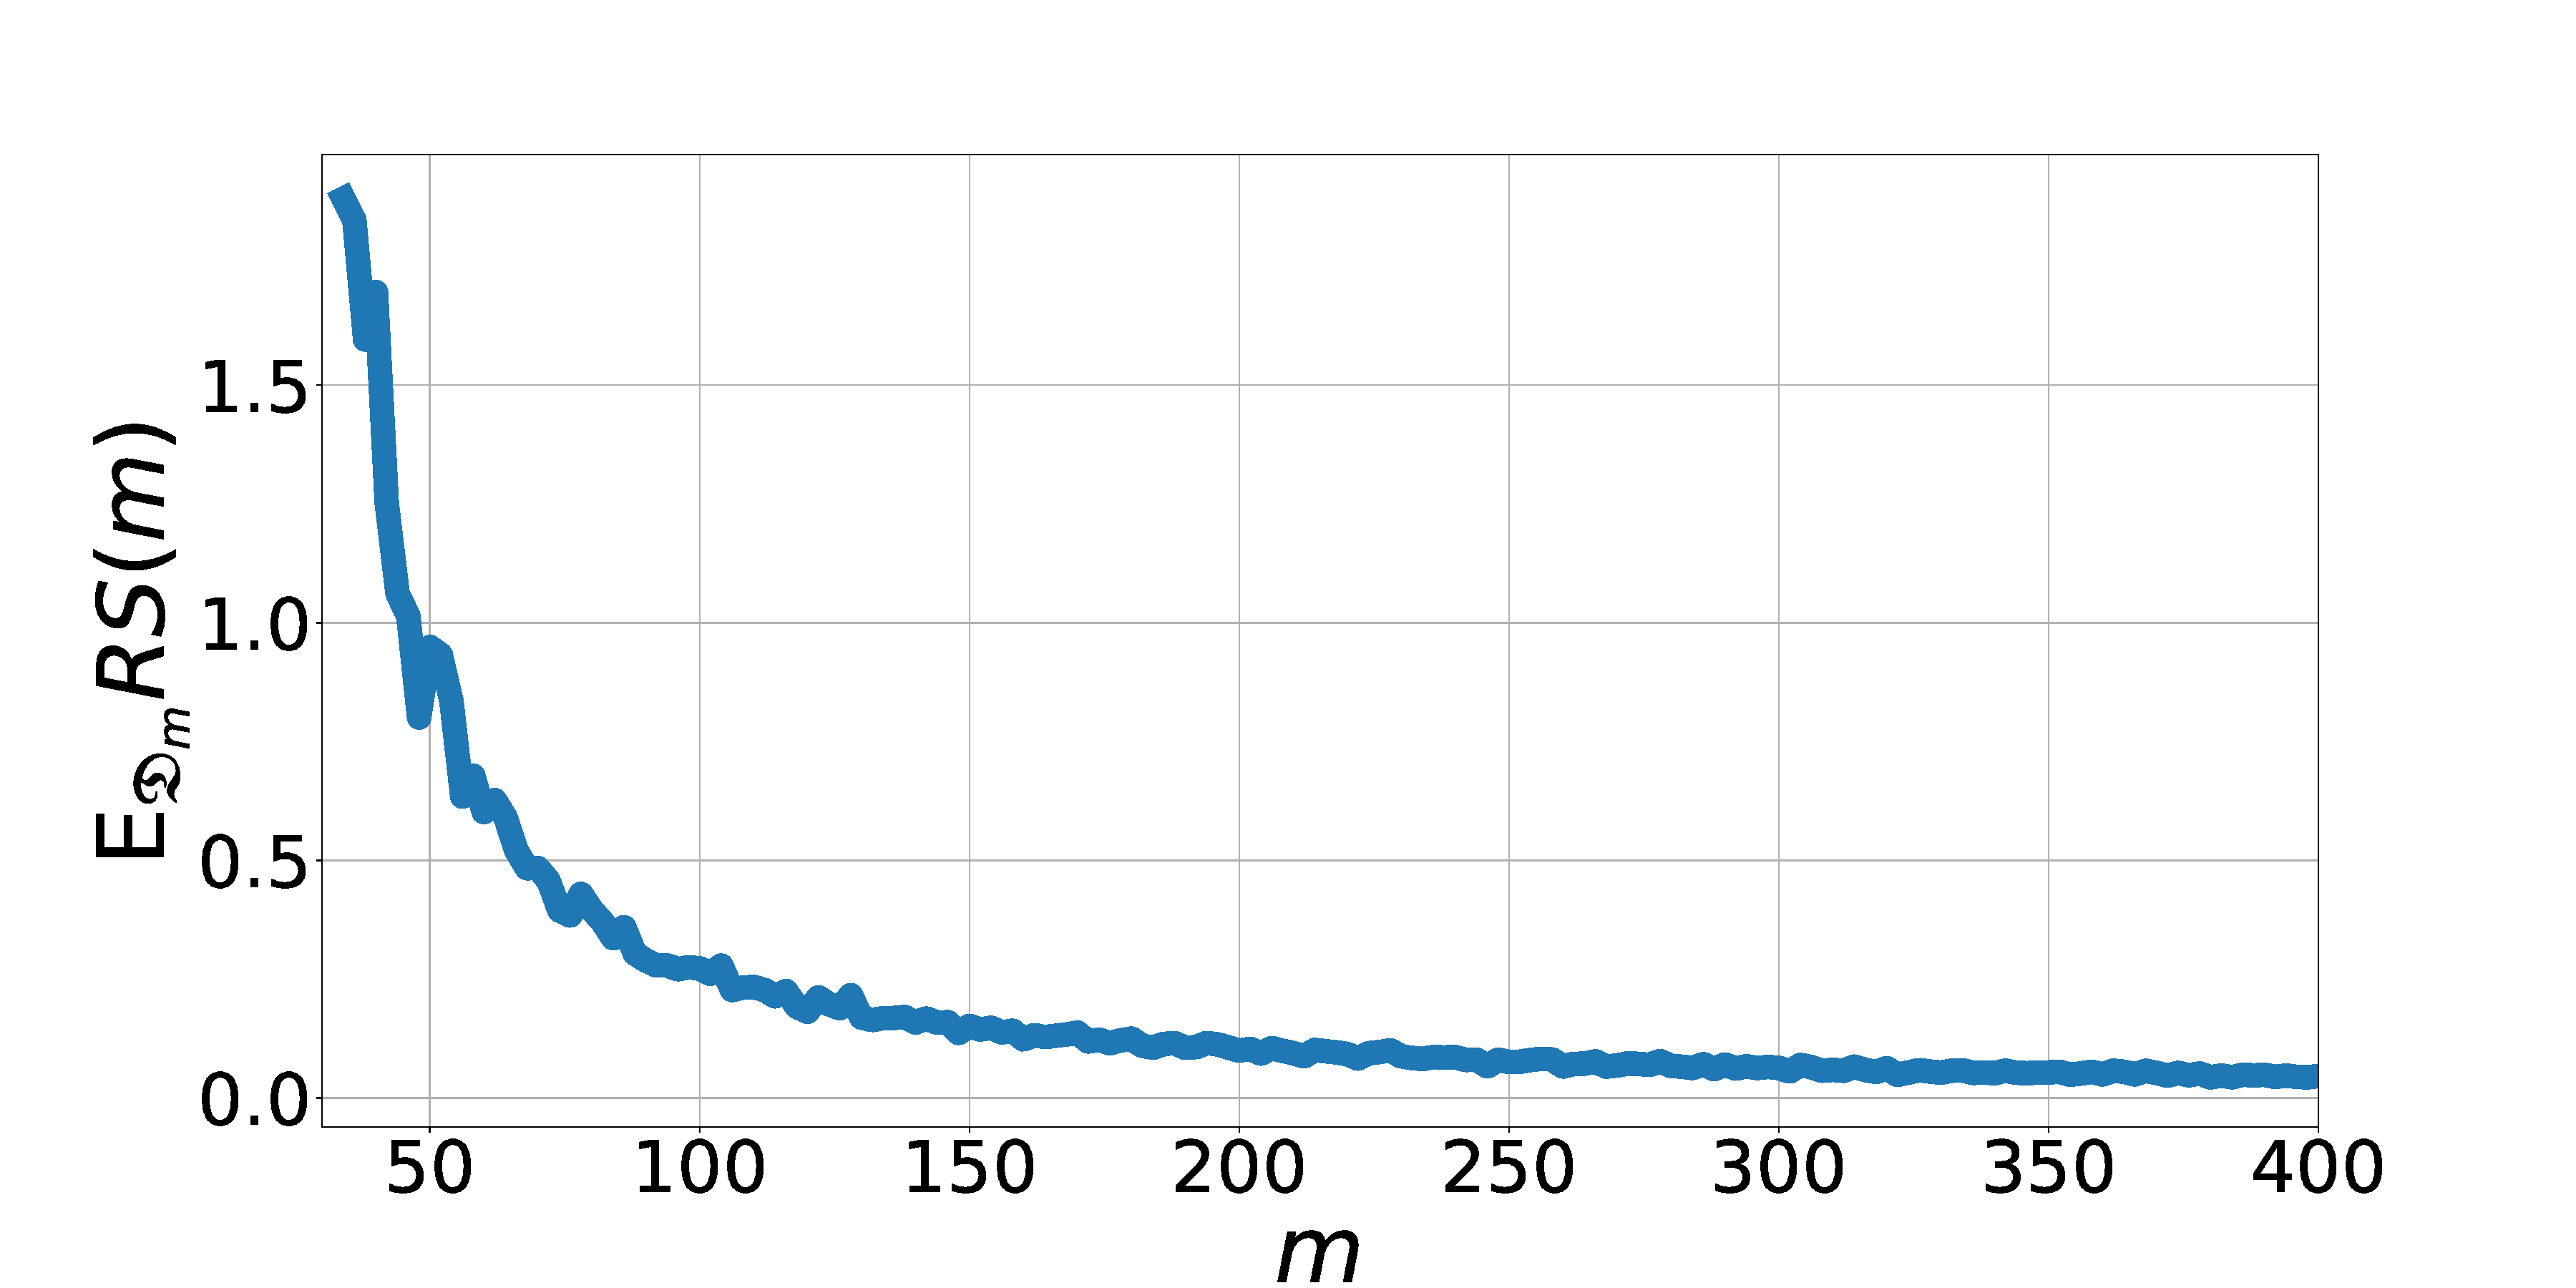
\includegraphics[width=0.49\textwidth]{results/samplesize/cross.pdf}
    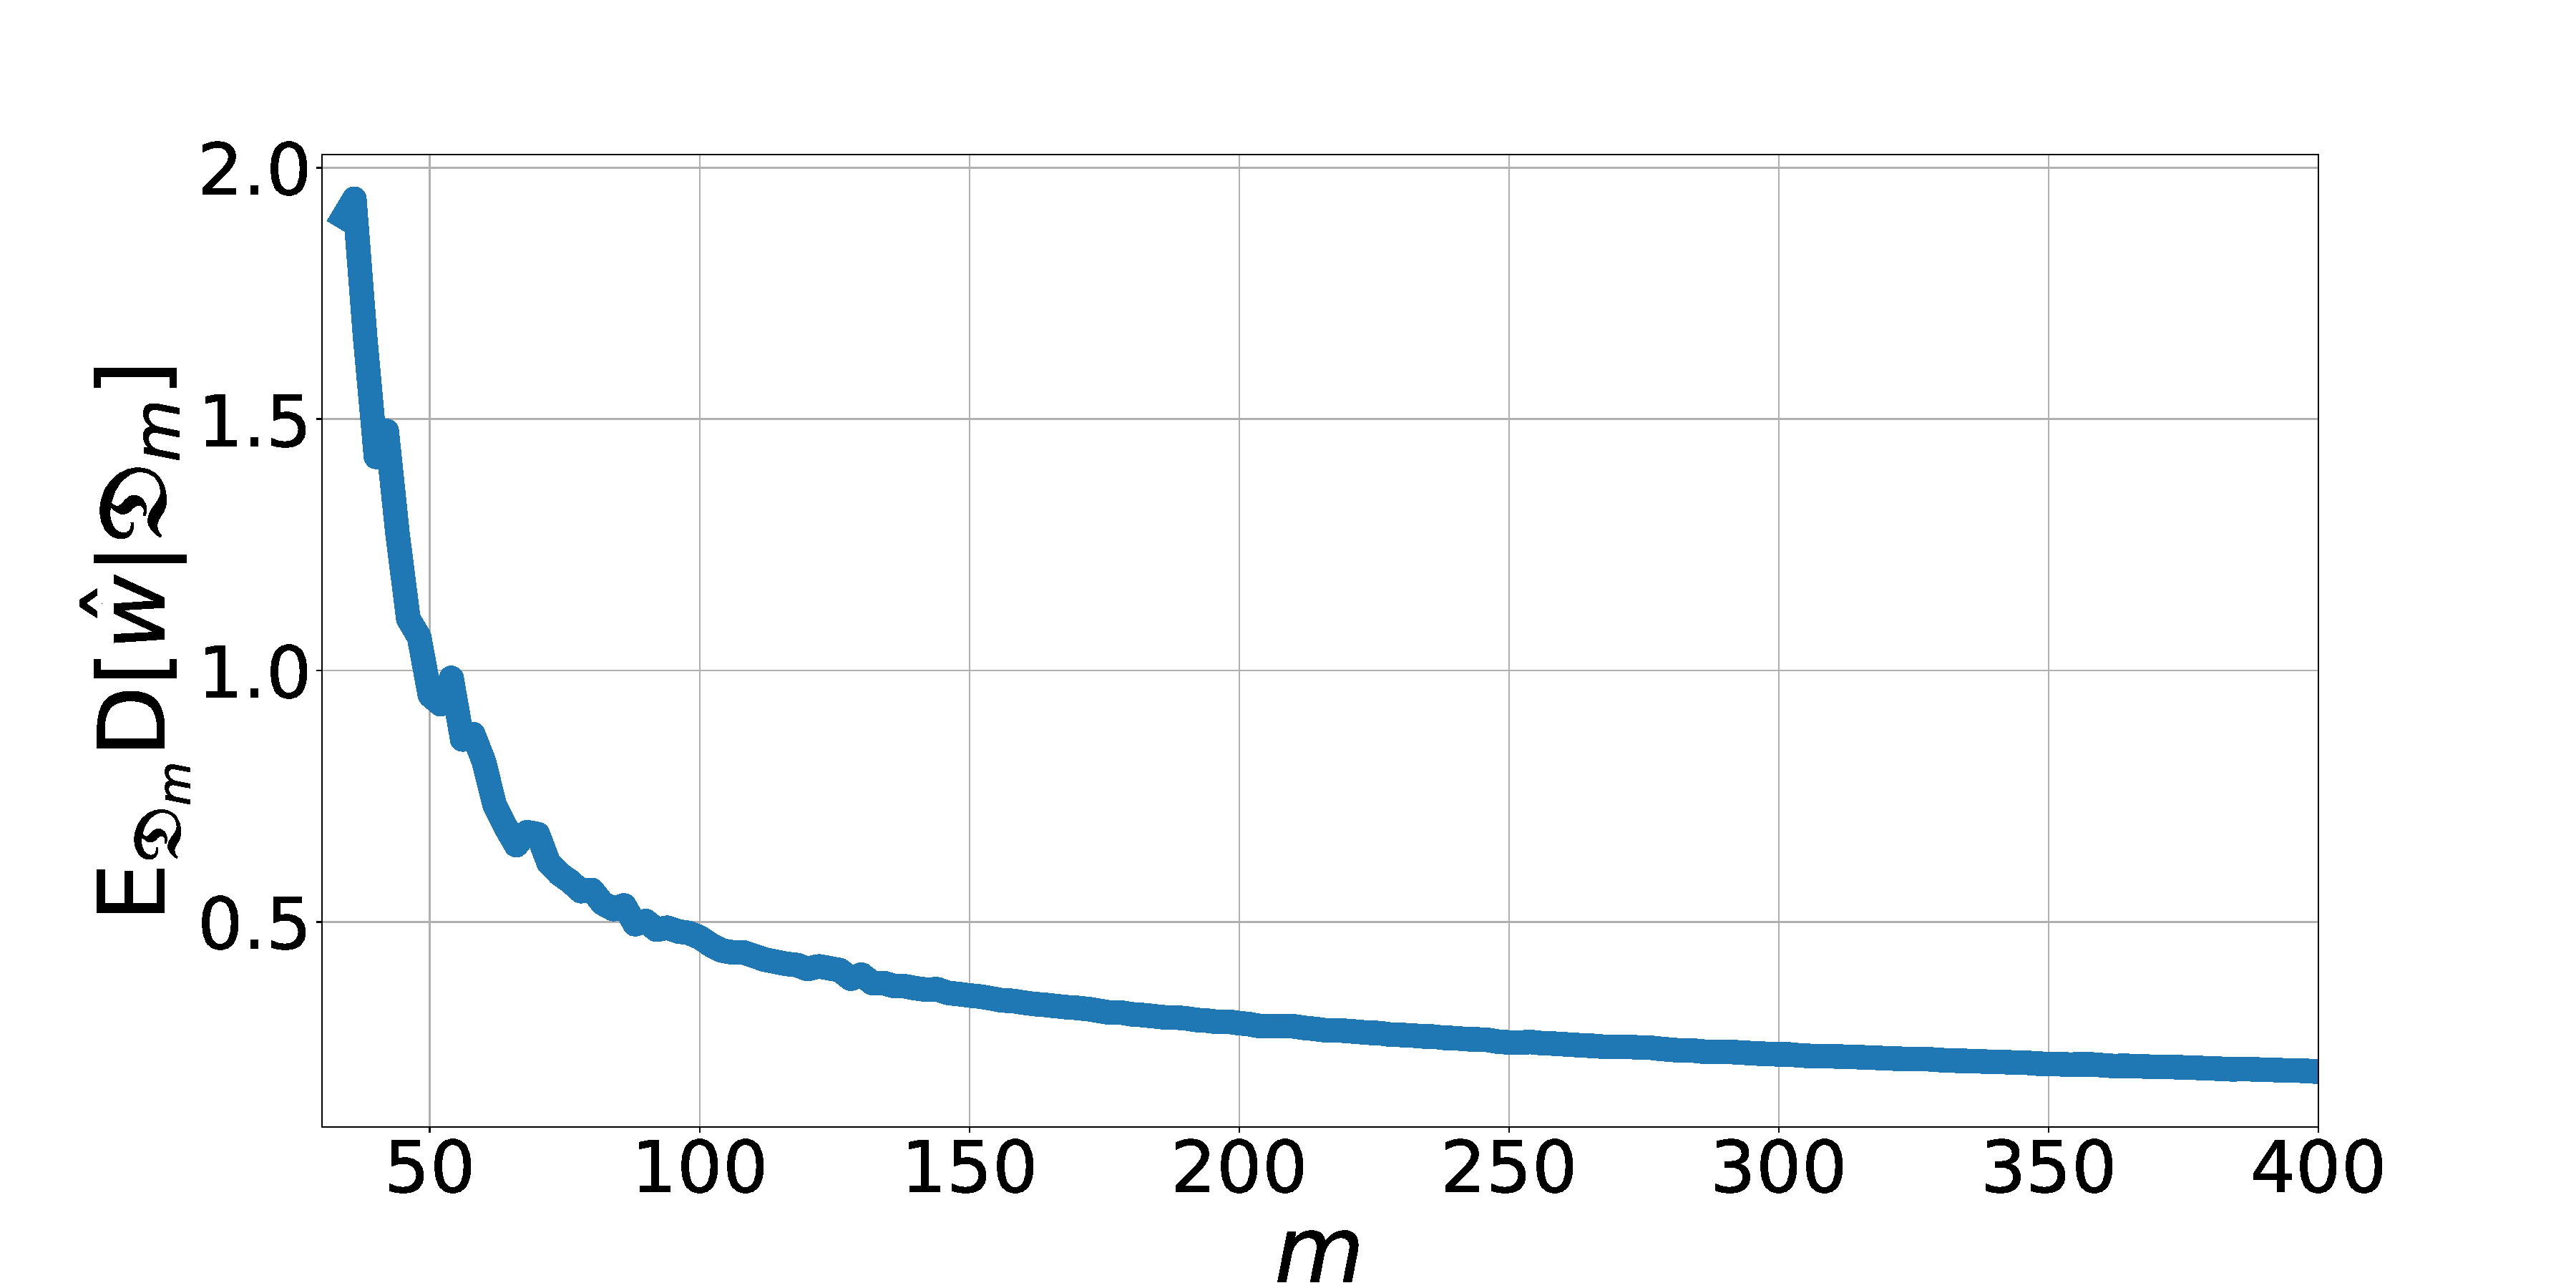
\includegraphics[width=0.49\textwidth]{results/samplesize/apvc.pdf}\\
    \includegraphics[width=0.49\textwidth]{results/samplesize/acc.pdf}
    \includegraphics[width=0.49\textwidth]{results/samplesize/alc.pdf}\\
    \includegraphics[width=0.49\textwidth]{results/samplesize/bootstrap.pdf}
    \includegraphics[width=0.49\textwidth]{results/samplesize/kl.pdf}\\
    \includegraphics[width=0.49\textwidth]{results/samplesize/maxu.pdf}
    \caption{Methods main scalar functions behaviour dependent on available sample size}
    \label{fig1}
\end{figure}

\begin{figure}[h!t]\center
    \includegraphics[width=0.85\textwidth]{results/samplesize/graphs.png}
    \caption{Methods behaviour depending on the available sample size}
    \label{fig2}
\end{figure}
    
The Figure~\ref{fig1} shows the dependence of the static values of each method for a given dataset with a fixed sample size $m$. The thresholds for each method are set expertly, which allows us to control different features of the dataset. The figure~\ref{fig1} demonstrates the adequacy of different definitions of sample size sufficiency. All the presented function are monotonous and all of them are asymptotically tend to a constant.
The Figure \ref{fig2} shows methods' results on samples of different size. It shows how methods differ in variance of computed $m^*$ and behaviour in case of small sample set. The methods converge and the result become independent of sample size from some value of $m$. 
    
Small variance interpret as stability of the methods output with little dependency on a particular subsample of some size. Some of the methods can not give estimation of sufficient sample size if they don't have such sample. That means that they are useless in terms of prediction, but can be used for retrospection and analysis of already conducted experiment.

%--- start inclusion
The dependence between the sample size estimation with the help of a certain method and the volume of data available to this method were considered in this exepriment. The constant achieved by the dependence diagram $m^*$ on $m$ is the forecast of the optimal sample size method. If this constant is less than $m$ where the diagram achieved it, then the method forecasts the optimal sample size before obtaining it. Only Lagrange, Wald methods, and the likelihood ratio method have such property.

The alteration of the sample size estimation depending on the alteration of certain hyperparameters for Bayesian methods, as well as the methods based on cross-validation and bootstrap is investigated in this experiment. In order to analyse the methods behaviour, see the sample {Boston Housing}, the other samples have the identical tendency.

Bayesian methods, as well as the methods based on cross-validation and bootstrap work on the basis of a certain decision rule for a certain sample function. In the Figure~\ref{fig1}, the dependence of these functions on the subsample size is shown. As shown in the Figure~\ref{fig1}, these functions are monotonically decreasing, or increasing. The function type of behaviour depends on the method. By altering the restrictions set by the application task, the sample size which will comply with these restrictions can be altered.
%--- end inclusion

\newpage

\section{Аппроксимация кривых второго порядка при помощи обучения с экспертом}
\subsection{Описание задачи}
\label{intro}
Interpretable model building in machine learning~(Ribeiro et al. 2016) is one of the key challenges.
Modern solutions of the image classification problem based on deep learning networks ResNet, VGG, Intercept~(Kaiming et al. 2016) are poorly interpreted models.
The papers~(Han et al. 2020; Akhtar et al. 2018) show that deep learning networks are sensitive even to small noise in the data, which is due to their uninterpretability.

In this paper, we propose a \textit {training with an expert} method.
This method assumes the use of subject knowledge of experts to improve the quality of approximation, as well as to obtain interpretable machine learning models.
The subject knowledge of experts about the sample will be called~\textit {expert information}.
It is assumed that the use of expert information allows the sample to be approximated by simple interpretable models, such as linear models. Machine learning methods that take expert knowledge into account when building models are called~\textit {expert learning}.

This paper solves the problem of approximating second-order curves on a contour image. Second-order curves are selected for analysis, since they are easily described by linear models. In this case, these figures need to be restored in such applied problems as the problem of recognizing the iris of the eye~(Matveev 2010; Matveev et al. 2014; Bowyer et al. 2010), the problem of describing the particle track in the hadron collider~(Salamani et al. 2018). Expert information about a second-order curve allows you to map points on a plane into a new feature description, where each curve is approximated by one linear model. A model that approximates one curve is called a \textit {local model}. To approximate the entire contour image, it is required to approximate several second-order curves using several local models. In this paper, the following restrictions on images are introduced: a) the image consists only of second-order curves; b) the image is approximated by a small number of second-order curves; c) the number and type of curves in the image is known.

\begin{figure}[h!]
     \includegraphics[width=\textwidth]{results/priorexpertfig/explanation}
     \caption {Example: a) expert information of the first expert; b) baseline data; c) expert information of the second expert}
    \label{intro:fig2}
\end{figure}

Figure~\ref{intro:fig2} shows an example of second-order curves, as well as expert information on curves. Figure~\ref{intro:fig2} a shows the expert information of the first expert. Using this information, the first curve is fitted with a linear model and the second curve is noise. Figure~\ref{intro:fig2} b shows the expert information of the second expert. Using this information, the second curve is fitted with a linear model and the first curve is noise.

When approximating several curves on one contour image, a multi-model is built. An example of multi-models is a random forest~(Chen et al. 2012), tree boosting~(Chen et al. 2016), a mixture of experts~(Yuksel et al. 2012). In this paper, a mixture of experts is considered as a multi-model. Expert mixture is a multi-model that linearly weights local models that approximate a portion of the sample. The values of the weighting coefficients depend on the object for which the prediction is made. To solve the problem of a mixture of experts, a variational EM-algorithm~(Dempster et al. 1997; Bishop 2010; Peng et al. 1996) is used. The mixture of experts has many uses in a number of applications. In the paper~(Estabrooks et al. 2001), the text classification problem is solved. In the papers~(Cheung et al. 1995; Weigend et al. 2000; Cao 2003; Mossavat et al. 2010; Sminchisescu C et al. 2007; Tuerk 2001; Yumlu et al. 2003), a mixture of experts is used to predict time series for speech recognition, daily human activity, and prediction of the value of securities. In the paper~(Ebrahimpour et al. 2009), a mixture of experts was considered to solve the problem of recognizing handwritten numbers in images.

As an example, the problem of approximation of the iris image is considered. Figure~\ref{intro:fig1:real} shows an example of the image that needs to be approximated. In this paper, we consider a processed image, which is given in outline form, an example of such an image is shown in Figure~\ref{intro:fig1:outer}. Figure~\ref{intro:fig1:outer} shows two local circle models that approximate the iris of the eye. Circumferences are a simple example of a second order curve.

\begin{figure}[h!]
	\subfloat[]{\includegraphics[height = 0.2\textheight]{results/priorexpertfig/real_image}\label{intro:fig1:real}} 
	\subfloat[]{\includegraphics[height = 0.2\textheight]{results/priorexpertfig/outline_image}\label{intro:fig1:outer}} 
\caption{An example of the image of the iris of the eye and its outline representation: a) the image of the iris of the eye; b) contour image of the iris and approximating the given image of the circumferences}
\label{intro:fig1}
\end{figure}

For the problem of approximating the iris of the eye, the following expert information is used: the iris of the eye is approximated by two concentric circumferences. Expert information is used to construct a feature description of plane points, as well as to build an optimization function. The part of the error function for optimization that uses expert information is called a regularizer. Thus, the information that the image of the circumferences is specified by the feature description, and the information that the concentric circumferences are specified using a special regularizer.

In a computational experiment, the quality of the approximation of the contour image is analyzed depending on the specified expert information and on the noise level in the synthetically generated data. The analysis of the quality of the approximation of the iris is carried out, depending on the amount of expert information that was used to build the model. Note that each approximated image is a separate set of points that need to be approximated.

\subsection{Постановка задачи поиска параметров кривых второго порядка}
\label{sec:1}
Binary image is set:
$$ \mathbf{M} \in \{0, 1 \}^{m_1\times m_2},$$
where 1 corresponds to the black point of the image, and 0 corresponds to the white point of the background.
From the image $\mathbf {M} $, a sample$ \mathbf{C}$ is constructed, the elements of which are the coordinates $(x_i, y_i)$ of black points: $$\mathbf{C} \in \mathbb{R}^{N \times 2}. $$
The expert assumes that the image consists of a second-order curve~$\Omega$.
Let for a set of points $\mathbf {C} \in \mathbb {R}^{N \times 2} $ that form a curve $\Omega, $ expert information about the figure $E(\Omega) $is given.
The set $E (\Omega)$ consists of the shape $\Omega$ expected by the expert and the set of its admissible transformations. Based on the expert description, let us introduce mappings into a new problem for approximation:
\begin{equation}\label{eq1}
	K_{x}\bigl(E(\Omega)\bigr): \mathbb{R}^{2} \rightarrow \mathbb{R}^{n}, \quad K_{y}\bigl(E(\Omega)\bigr): \mathbb{R}^{2} \rightarrow \mathbb{R},
\end{equation} 
where~$K_{x}$ mapping objects to the attribute description of objects,~$n$is the number of features, and~$K_ {y}$ is a mapping to a target variable for an object. Applying the mappings~$K_ {x}, K_{y}$for the sample~$\mathbf {C}$ element by element we obtain:
\begin{equation}
\label{eq2}
	K_{x}\bigl(E(\Omega\bigr), \mathbf{c}) = \mathbf{x}, \quad  K_{y}\bigl(E(\Omega), \mathbf{c}\bigr) = y,
\end{equation}
where~$\mathbf{c} = (x_i, y_i)$ is a sample point $\mathbf{C}$.

Applying the mappings \eqref{eq2} to the original set of points $\mathbf {C} $, we obtain the sample
\begin{equation}
\label{eq4}
    \mathfrak{D} = \{(\mathbf{x}, y) \; | \; \forall \mathbf{c} \in \mathbf{C} \; \mathbf{x} = K_x(\mathbf{c}), \; y = K_y(\mathbf{c}) \}.
\end{equation}

We get that the original problem of curve approximation~$\Omega$ is reduced to approximation of the sample~$\mathfrak {D}$. In this paper, it is assumed that the sample~$\mathfrak {D}$ is approximated by a linear model:
\begin{equation}
	g(\mathbf{x}, \mathbf{w}) = \mathbf{x}^\mathsf{T} \mathbf{w},
\end{equation} 
where~$\mathbf{w}$ vector, the parameter to be found.

To find the optimal vector of parameters~$\hat {\mathbf {w}}$, it is required to solve the following optimization problem:
\begin{equation}
	\hat{\mathbf{w}} = \arg\min_{\mathbf{w}\in\mathbb{R}^n} \sum_{\left(\mathbf{x}, y\right) \in \mathfrak{D}}\|g(\mathbf{x}, \mathbf{w}) - y \|_2^2.
\end{equation} 

Thus, the problem of approximating the original curve~$\Omega$ is reduced to solving the problem of linear regression, i.e. finding the components of the vector $\hat{\mathbf {w}}$ connecting the resulting $\mathbf {x}$ and $y$.

In the case when on the image $K$ the second-order curves  $\Omega_1, \dots, \Omega_K$, for each of which there is expert information $E_k = E (\Omega_k), \, k \in \{1, \dots , K\}$, the problem of constructing a multi-model called a mixture of $K$ experts is posed.
\begin{definition}
We call the multimodel $ f $ a mixture of K experts
\begin{equation}
	f = \sum\limits_{k = 1}^{K}\pi_k(\mathbf{x}, \mathbf{V})g_k(\mathbf{w}_k),  \quad \pi_k(\mathbf{x}, \mathbf{V}): \mathbb{R}^{n\times |\mathbf{V}|} \rightarrow [0, \, 1], \quad \sum\limits_{k = 1}^{K}\pi_k(\mathbf{x}, \mathbf{V}) = 1, 
\end{equation}
where $g_k$ is a local model called by the expert, $\mathbf{x}$is an attribute description of an object, $\pi_k$is a gateway function, the vector $\mathbf{w}_k$ are local model parameters, the vector $\mathbf{V}$ are gateway function parameters. In this paper, $g_k$ is a linear model.
\end{definition}

For each second-order curve, mappings (\ref{eq1}) are given. For convenience, we introduce the following notation: $K_x^k\bigr(\mathbf{c}\bigr) = K_x\bigr(\Omega_k, \mathbf{c}\bigr)$ and $K_y^k\bigr(\mathbf{c}\bigr) = K_y\bigr(\Omega_k, \mathbf{c}\bigr)$. Then, using local linear models, we construct a universal multi-model describing the curves $\Omega_1, \dots, \Omega_K$ on the image $\mathbf{M}$:
\begin{equation}
\label{5}
	f = \sum\limits_{\mathbf{c} \in \mathbf{C}} \sum_{k = 1}^{K} \pi_k(\mathbf{c}, \mathbf{V})g_k(K^k_{x}\bigl(\mathbf{c}), \mathbf{w}_k), 
\end{equation}
where $\pi_k$ is the  gateway function. In this paper, we consider a simple case, where~$\mathbf{x}=K^1_{x}\bigl(\mathbf{c})=\cdots=K^K_{x}\bigl(\mathbf{c}),$ then the expression~\eqref{5} is rewritten in the following simple form:
\begin{equation}
\label{5_1}
	f = \sum\limits_{\mathbf{c} \in \mathbf{C}} \sum_{k = 1}^{K} \pi_k(\mathbf{x}, \mathbf{V})g_k(\mathbf{x}, \mathbf{w}_k), 
\end{equation}
where the gateway function $\pi_k$ has the following form:
\begin{equation}
\label{6}
	\pi_k(\mathbf{x}, \mathbf{V}): \mathbb{R}^{n\times |\mathbf{V}|} \rightarrow [0, \, 1], \; \; \; \; \sum\limits_{k = 1}^{K}\pi_k(\mathbf{x}, \mathbf{V}) = 1,
\end{equation}
where $\mathbf{V}$ are the gateway function parameters, and $g_k$ is a local model.
    
In this paper
\begin{equation}
    \boldsymbol{\pi}(\mathbf{x}, \mathbf{V}) = \text{softmax}\bigl(\mathbf{V}_1^{\mathsf{T}}\boldsymbol{\sigma}(\mathbf{V}_2^{\mathsf{T}}\mathbf{x}) \bigr),
\end{equation}
where $\mathbf{V} = \{ \mathbf{V}_1, \, \mathbf{V}_2\}$ are the gateway function parameters,
$\mathbf{V}_1 \in \mathbb{R}^{p \times k}, \, \mathbf{V}_2 \in \mathbb{R}^{n \times p}$. 

To find the optimal parameters of the multi-model, it is necessary to solve the following optimization problem:
\begin{equation}\label{9}
\mathcal{L} = \sum\limits_{(\mathbf{x}, y) \in \mathfrak{D}} \sum\limits_{k = 1}^{K} \pi_k(\mathbf{x}, \mathbf{V})(y - \mathbf{w}_k^{\mathsf{T}}\mathbf{x})^2 + R\bigl(\mathbf{V}, \mathbf{W}, E(\Omega)\bigr) \rightarrow \min_{\mathbf{V}, \mathbf{W}},
\end{equation}
where $\mathbf{W} = [\mathbf{w}_1, \dots, \mathbf{w}_k]$ are  parameters of local models, $R\bigl(\mathbf{V}, \mathbf{W}, E(\Omega)\bigr)$ is regularization parameters, based on expert information.

\subsection{Построение признакового описания фигур}
\label{sec:3}
\paragraph{ Unified space for second-order curves.} An arbitrary second-order curve, the main axis of which is not parallel to the ordinate axis, is given by the following expression:
\[
\label{st:coef}
x^2 = B'xy+C'y^2+D'x+E'y+F',
\]
where the coefficients $B ', C'$ are subject to restrictions that depend on the type of the curve. The expression~\eqref{eq2} takes the following form:
\[
\label{st:K_map}
K_x\bigr(\mathbf{c}_i\bigr)=\left[x_iy_i, y_i^2, x_i, y_i, 1\right], \quad K_y\bigr(\mathbf{c}_i\bigr)=x_i^2,
\]
whence we obtain the linear regression problem for recovering the parameters~$ B ', C', D ', E', F '$ from the selected sample.

\paragraph{ Circumference.} As a special case of a second-order curve, we consider the circumference.
Let $(x_0, y_0)$ be the center of the circumference to be found on the binary image $\mathbf {M} $, and $r$ be its radius.
The sample elements $(x_i, y_i) \in \mathbf {C}$ are the locus of points, which is approximated by the equation of the circumference:
\begin{equation}
(x_i - x_0)^2 + (y_i - y_0)^2 = r^2.
\end{equation}
Expanding the brackets, we get:
\begin{equation}(2x_0)\cdot x_i + (2y_0)\cdot y_i + (r^2 - x_0^2 - y_0^2)\cdot 1 = x_i^2 + y_i^2 . 
\end{equation}
Then the presentations (\ref{eq2}) take the following form:
\begin{equation}
\label{10}
K_{x}(\mathbf{c}_i) = [x_i, \, y_i, \, 1] = \mathbf{x}, \,  K_{y}(\mathbf{c}_i) = x_i^2+y_i^2 = y.
\end{equation} 
Assign the linear regression problem \eqref{eq4}.
Vector components $\mathbf{w} = [w_0, \, w_1, \, w_2]^\mathsf{T}$, binding $\mathbf{x}$ and $y$, restore the parameters of the circumference: \begin{equation} x_0 = \frac{w_0}{2}, \; y_0 = \frac{w_1}{2}, \; r = \sqrt{w_3 + x_0^2 + y_0 ^2}.\end{equation}

\subsection{Композиция фигур}
\label{sec:4}
o construct a composition of figures, we will use the expression~\eqref{9}, which takes the following form:
\begin{equation} 
\label{statment:optim:task}
\begin{aligned}
\mathcal{L} = \sum\limits_{\mathbf{c} \in \mathbf{C}} \sum\limits_{k = 1}^{K} \pi_k(\mathbf{c}, \mathbf{V})\left(K^{k}_y\bigr(\mathbf{c}\bigr) - \mathbf{w}_k^{\mathsf{T}}K^{k}_x\bigr(\mathbf{c}\bigr)\right)^2 + R\bigl(\mathbf{V}, \mathbf{W}, E(\Omega)\bigr) \rightarrow \min_{\mathbf{V}, \mathbf{W}},
\end{aligned}
\end{equation} 
where~$K^{k}_x, K^{k}_y$ expert representation of the~$k$-th expert. Assuming that all curves in the image are described by one attribute description $\mathbf {x} =K^{1}_x\bigr(\mathbf{c}\bigr)=\cdots=K^{K}_x\bigr(\mathbf{c}\bigr), x= K^{1}_y\bigr(\mathbf{c}\bigr)=\cdots=K^{K}_y\bigr(\mathbf{c}\bigr),$ we get the following optimization problem:
\begin{equation} 
\label{statment:optim:task:simp}
\begin{aligned}
\mathcal{L} = \sum\limits_{\left(\mathbf{x}, y\right) \in \mathfrak{D}} \sum\limits_{k = 1}^{K} \pi_k(\mathbf{x}, \mathbf{V})\left(y - \mathbf{w}_k^{\mathsf{T}}\mathbf{x}\right)^2 + R\bigl(\mathbf{V}, \mathbf{W}, E(\Omega)\bigr) \rightarrow \min_{\mathbf{V}, \mathbf{W}},
\end{aligned}
\end{equation} 

As a regularizer~$R$, additional restrictions on the vectors of model parameters are considered. To solve the optimization problem~\eqref{statment:optim:task:simp} it is proposed to use the EM-algorithm.

\subsection{Вычислительный эксперимент}
\label{sec:5}

A computational experiment was carried out to analyze the quality of models of second-order curves in the image. The experiment is divided into several parts. The first part is an experiment with several circumferences in the image. The second part analyzes the convergence of the method depending on the noise level in the data and on the specified expert information. In the third part, an experiment is conducted to approximate the iris of the eye.

\begin{figure}[h!]
	\subfloat[]{\includegraphics[height = 0.2\textheight]{results/priorexpertfig/900.eps}} 
	\subfloat[]{\includegraphics[height = 0.2\textheight]{results/priorexpertfig/901.eps}}
	\subfloat[]{\includegraphics[height = 0.2\textheight]{results/priorexpertfig/902.eps}} 

\caption{Multi-model depending on different prior assumptions and noise level. From left to right: circumferences without noise; noise in the radius of the circle; noise in the radius of a circle as well as arbitrary points throughout the image.}
\label{ce:fig3}
\end{figure}

\begin{figure}[h]
	\subfloat[]{\includegraphics[height = 0.2\textheight]{results/priorexpertfig/900noise.eps}} 
	\subfloat[]{\includegraphics[height = 0.2\textheight]{results/priorexpertfig/901noise.eps}}\\
	\subfloat[]{\includegraphics[height = 0.2\textheight]{results/priorexpertfig/902noise.eps}} 

\caption{Dependence of the parameters  $r$, $x_0$ and $y_0$ on the iteration number for different prior distributions. From left to right: circumferences without noise; noise in the radius of the circle; noise in the radius of a circle as well as arbitrary points throughout the image.}
\label{ce:fig4}
\end{figure}

In this part of the experiment, an example of training a multi-model is shown to approximate several second-order figures simultaneously. A synthetic sample is used as data, which is obtained by generating three arbitrary non-intersecting circumferences, as well as adding noise to these circumferences. Noise was added to the radius of the circle for each point, and random points were added to the sample that do not belong to circumstances.

Figure~\ref{ce:fig3} shows the result of building an ensemble of locally approximating models that approximate the sample. Each local model approximates one circumference, and when adding different noise, the quality of the approximation will drop.
Figure~\ref{ce:fig4} shows a graph of the dependence of the radius of the circumferences $r$ and their centers $(x_0, y_0)$ on the iteration number. 

\begin{figure}[h!t]
\includegraphics[width=0.8\textwidth]{results/priorexpertfig/beta_gamma}
\caption{ The result of the approximation for data with different noise levels~$\beta$ and on the variance of the prior distribution~$\gamma$}
\label{ce:fig6}
\end{figure}

\begin{figure}[h!t]
\includegraphics[width=0.5\textwidth]{results/priorexpertfig/3dplot}
\caption{Dependence of models on the noise level~$\beta$ in the data, as well as on the variance of the prior distribution~$\gamma$}
\label{ce:fig5}
\end{figure}
In this part of the experiment, we analyze the quality of approximation~$S$ on the noise level~$\beta$ in the data and on the parameter of a priori distributions~$\gamma$. The sample is obtained as followsfirst, two vectors of parameters are randomly selected~$\mathbf{w}^\text{true}_{1}$ and~$\mathbf{w}^\text{true}_{2}$ are  coefficients of two parabolas. The vectors~$\mathbf {w}^\text {true}_{1} $ and~$\mathbf{w}^\text {true}_{2} $ are used to generate points~$x_i$ and~$y_i$ with normal noise added~$\varepsilon\sim\mathcal {N} \bigr(0,\beta\bigr)$. When training a multi-model, the prior distribution of parameters is considered~$\mathbf{w}_1\sim\mathcal{N}\bigr(\mathbf{w}^\text{true}_{1}, \gamma\mathbf{I}\bigr),\mathbf{w}_2\sim\mathcal{N}\bigr(\mathbf{w}^\text{true}_{2}, \gamma\mathbf{I}\bigr)$.

The following quality criterion is considered:
\[
S = ||\mathbf{w}^\text{pred}_{1} - \mathbf{w}^\text{true}_{1}||^{2}_{2} + ||\mathbf{w}^\text{pred}_{2} - \mathbf{w}^\text{true}_{2}||^{2}_{2},
\]
where~$\mathbf{w}^\text{pred}_{1}$ approximation of the vector of parameters of the first local model, and~$\mathbf{w}^\text{pred}_{2}$ approximation of the vector of parameters of the second local model.

Figure~\ref{ce:fig5} shows the dependence of the quality criterion~$S$ on the noise level~$\beta$ and the a priori distribution parameter~$\gamma$. The graph shows that at a low noise level~$\beta$ the quality of the approximation does not depend on the parameter~$\gamma $, and with an increase in the noise~$\beta $ the quality of the approximation~$S$ decreases.

Figure~\ref{ce:fig5} shows an example of how the algorithm works with different parameters~$\beta$ and $\gamma$. It is seen that in the absence of noise~$\beta$, both local models approximate the sample. With an increase in the noise level, the quality of the approximation decreases: at~$\beta = 0 {,}2$, with an increase in $\gamma$, the first local model from a parabola goes over to an ellipse; for~$\beta=0 {,}4$ as $\gamma$ increases, the first local model from a parabola goes over to an ellipse, and the second model from a parabola goes over to a hyperbola.

\begin{figure}[h!]
	\subfloat[]{\includegraphics[height = 0.17\textheight]{results/priorexpertfig/not_prior_real_example}} 
	\subfloat[]{\includegraphics[height = 0.17\textheight]{results/priorexpertfig/prior_real_example}}
	\subfloat[]{\includegraphics[height = 0.17\textheight]{results/priorexpertfig/prior_regular_real_example}} 
\caption{Visualization of the approximation of the iris: a) if the $ R_0 $ regularizer is specified; b) if the $ R_1 $ regularizer is specified; b) if the $ R_2 $ regularizer is specified}
\label{ce:fig6}
\end{figure}


\begin{figure}
     \includegraphics[width=\textwidth]{results/priorexpertfig/experiment_real_not_prior}\\
     \caption{Visualization of the multi-model convergence process in the case of a regularizer~$R_0$}
    \label{ce:fig7}
\end{figure}

\begin{figure}
     \includegraphics[width=\textwidth]{results/priorexpertfig/experiment_real_prior}
     \caption{Visualization of the multi-model convergence process in the case of a regularizer~$R_1$}
    \label{ce:fig8}
\end{figure}

\begin{figure}
     \includegraphics[width=\textwidth]{results/priorexpertfig/experiment_real_regular}
     \caption{Visualization of the multi-model convergence process in the case of a regularizer~$R_2$}
    \label{ce:fig9}
\end{figure}

An analysis of the quality of the approximation is carried out for the problem of approximating the iris of the eye in the image. The iris of the eye consists of two concentric circumferences, therefore, a multi-model is considered, which consists of two experts: each expert approximates one of the circumstances. In a computational experiment, the quality of the approximation of circumferences is compared in the case of specifying different regularizers $R_0, R_1, R_2$. Regularizer$R_0\bigl(\mathbf{V}, \mathbf{W}, E(\Omega)\bigr)=0,$ that is, there is no regularizer. Regularizer:
\[
R_1\bigl(\mathbf{V}, \mathbf{W}, E(\Omega)\bigr)= -\sum_{k=1}^{K}\mathbf{w}_k^{\mathsf{T}}\mathbf{w}_k,
\]
which romotes near-zero parameters of local models.
Regularizer 
\[
R_2\bigl(\mathbf{V}, \mathbf{W}, E(\Omega)\bigr)= -\sum_{k=1}^{K}\mathbf{w}_k^{\mathsf{T}}\mathbf{w}_k + \sum_{k=1}^{K}\sum_{k'=1}^{K}\sum_{j=1}^2\left(w_k^j-w_k'^j\right)^2,\]
which promotes the coincidence of the centers of the circumferences and close to zero parameters of the model.
Figure~\ref{ce:fig6} shows the result of the eye iris approximation algorithm after 10 iterations. It can be seen that in the absence of a regularizer, one of the circumferences is found incorrectly. If the regularizer~$R_1 $ is given, the model approximates both circumferences with good quality, but the circumferences are not concentric. In case of specifying the regularizer~$R_2$, we get concentric circumferences on the image.

Figure~\ref{ce:fig7}--\ref{ce:fig9} shows the process of convergence of multi-models in the case of specifying different regularizers~$R_0, R_1, R_2$. It can be seen that the models with the regularizer type~$R_1$ and~$R_2$ approximate both circumferences, and the multi-model with the$R_0$ regularizer approximates only the large circumference.

\newpage


\section{Локальные модели в задачах кластеризации временных рядов}
\subsection{Описание задачи}
Анализ физической активности человека производится при помощи мобильных телефонов, разумных часов~\cite{kwapisz2010, wang2014}. 
Эти устройства используют акселерометр, гироскоп и магнитометр. 
Цель данной работы заключается в  разметке и распознавании человеческой активности~\cite{Ignatov2015, Olivares2012, cinar2018}, а также поиска начала каждого действия~\cite{motrenko2015}. 
Примерами одного сегмента действия служит шаг, шаг бега, приседание, прыжок и др. 
Исследуются последовательности, которые состоят не менее чем из двух подряд идущих сегментов, которые соответствуют одному и тому жу типу человеческой активности.

\begin{figure}[h!t]\center
\subfloat[]
{\includegraphics[width=0.5\textwidth]{results/series/example}\label{example:1}}
\subfloat[]
{\includegraphics[width=0.5\textwidth]{results/series/example_phase}\label{example:2}}\\
\caption{Временной ряд, с разметкой на кластеры: a) временной ряд с ассесорской разметкой на кластеры и выделением начала квазипериодического сегмента; b) проекция фазовых траекторий на первые две главные компоненты }
\end{figure}

Временные ряды~---~это объекты сложной структуры. 
При их классификации значимую роль играет модель построения признакового пространства.
В данной работе объектом анализа и кластеризации является точка на оси времени. 
Решается задача кластеризации точек временного ряда. 
При \textit{кластеризации} каждой точке временного ряда ставится в соответствие метка из конечного множества меток. 
Каждая метка соответствует одному характерному физическому действию. \textit{Сегмент} это часть временного ряда, которая соответствует одному характерному физическому действию, например: шаг двумя ногами при ходьбе, или шаг двумя ногами при беге.
Последовательность сегментов, которые соответствуют одному физическому действия образуют \textit{цепочку} действий. 
Предполагается, что цепочка действий образует квазипериодическую последовательность значений временного ряда.
Последовательность точек $\{b_t\}_{t=1}^{N}$ назовем \textit{квазипериодической} с периодом $T$, если для всех $t$ найдется $\Delta$, такое что:
\begin{equation}
\label{eq:int:1}
\begin{aligned}
b_t \approx b_{t+T+\Delta}, \quad \left|\Delta\right| \ll T.
\end{aligned}
\end{equation}
Пример кластеризации и разбиения ряда на сегменты показан на рис.~\ref{example:1}. Данный ряд разбит на два характерных физических действия, которые обозначаются Type~1 и Type~2. Также данный ряд содержит в себе две квазипериодические цепочки действий.

Решение задачи кластеризации состоит из двух этапов. 
Во-первых, для получения признакового описания временного ряда предлагается алгоритм локальной аппроксимации временного ряда при помощи метода главных компонент~\cite{Shiglavsi1997}. 
Под \textit{локальной} аппроксимацией временного ряда подразумевается, что для признакового описания его точки используется не весь ряд, а только некоторая окрестность данной точки. 
В качестве признакового описания точки временного ряда рассматриваются две главные компоненты \textit{сегмента фазовой траектории} в окрестности данной точки.
На рис.~\ref{example:2} показаны две первые главные компоненты \textit{фазовых траекторий}, а также проекция фазовых траекторий на эти компоненты.
Они соответствуют разным физическим действиям, которые обозначаются Type~1 и Type~2, внутри одного временного ряда.
Как видно плоскости, которые порождены данными главными компонентами не совпадают. 
Это говорит о том, что наблюдаются различные действия. 
Во-вторых, вводится функция расстояния в построенном пространстве признакового описания. 
Данная функция является расстояниям между двумя базисами некоторых подпространств внутри всего фазового пространства временного ряда.
На рис.~\ref{example:2} данная функция является некоторым расстояниям между двумя плоскостями.
Получив расстояния между точками временного ряда, выполним кластеризацию данных точек.
Задача сегментации внутри каждого кластера решается при помощи метода, который рассмотрен в~\cite{motrenko2015}.

Для решения задачи кластеризации точек временного ряда вводятся предположения. 
Предполагается, что периоды различных сегментов различаются незначительно, причем известны минимальный и максимальный периоды сегмента и число различных сегментов внутри временного ряда. 
Также предполагается, что тип активности во времени не меняется часто, а также что фазовые траектории разных сегментов являются различными. 

Проверка и анализ метода кластеризации проводится на синтетической и реальной выборках. 
Синтетическая выборка построенная при помощи суммы нескольких первых членов ряда Фурье со случайными коэффициентами. 
Эксперимент по сегментации временного ряда проводился на простых синусоидальных сигналах с произвольной амплитудой и частотой. 
Реальные данные получены при помощи мобильного акселерометра, который снимал показания во время некоторой физической активности человека. 

В~\cite{kwapisz2010} рассматриавется метод построения признакового описания на основе экспертно заданых порождающих функций.
В~\cite{lukashin2003} рассматривается метод построения признаков на основе гипотезы порождения данных. 
В~\cite{Ivkin2015} рассматривается комбинированное признаковое описание на основе данных методов. 
В~\cite{Katrutsa2015} рассматривается проблема построение признакового пространства и предлагается критерий избыточности выбранных признаков.

Работа~\cite{motrenko2015} является ближайшей работой по данной теме. Она заключается в поиске начала сегмента внутри квазипериодического сигнала, который состоит, только из одной цепочки действий. Этот метод основан на исследовании фазового пространства, а именно поиска устойчивой гиперплоскости, которая делит фазовое пространство на две равные части. В качестве начала сегмента выбираются точки, которые находятся близко к данной гиперплоскости. В~\cite{motrenko2015} предлагается выполнить проекцию фазового пространства на первые две главное компоненты, после чего провести устойчивую прямую, выделив начала каждого сегмента. 
Данный метод имеет недостаток в том, что позволяет находить начало только для временного ряда, который состоит из квазипериодического сигнала единственного типа.


Также близкой является работа~\cite{cinar2018}.  Данная работа заключается в поиске периодической структуры внутри ряда при помощи модели LSTM с модифицированным механизмом Attention. Предполагается, что механизм Attention будет давать максимальное значение score в точках, которые удаленны от данной на целое количество периодов.

\subsection{Постановка задачи кластеризации точек временного ряда}

Задан временной ряд
\begin{equation}
\label{eq:st:1}
\begin{aligned}
\textbf{x} \in \mathbb{R}^{N},
\end{aligned}
\end{equation}
где~$N$ число точек временного ряда. Он состоит из последовательности сегментов:
\begin{equation}
\label{eq:st:2}
\begin{aligned}
\textbf{x} = [\textbf{v}_1, \textbf{v}_2, \cdots, \textbf{v}_M],
\end{aligned}
\end{equation}
где~$\textbf{v}_i$ некоторый сегмент из множества сегментов~$\mathbf{V}$, которые встречаются в данном ряде. 
Причем для всех~$i$ либо~$[\textbf{v}_{i-1},\textbf{v}_{i}]$ либо~$[\textbf{v}_{i},\textbf{v}_{i+1}]$  является цепочкой действий. Пусть множество~$\mathbf{V}$ удовлетворяет следующим свойствам:

\begin{equation}
\label{eq:st:3}
\begin{aligned}
\left|\mathbf{V}\right| = K, \quad \textbf{v} \in \mathbf{V}~\left|\textbf{v}\right| \leq T,
\end{aligned}
\end{equation}
где~$\left|\mathbf{V}\right|$ число различных действий в множестве сегментов $\mathbf{V},$~$\left|\textbf{v}\right|$ длина сегмента, а~$K$ и~$T$ это число различных действий во временном ряде и длина максимального сегмента соответсвенно.

Рассматривается отображение
\begin{equation}
\label{eq:st:4}
\begin{aligned}
a : t \to \mathbb{Y} = \{1,\cdots, K\}, 
\end{aligned}
\end{equation}
где~$t \in \{1,\cdots, N\}$ некоторый момент времени, на котором задан временной ряд.
Требуется, чтобы отображение~$a$ удовлетворяло следующим свойствам:

\begin{equation}
\label{eq:st:5}
\begin{aligned}
\begin{cases}
    a\left(t_1\right) = a\left(t_2\right), &  \text{если в моменты } t_1, t_2 \text{ совершается один тип действий}\\
    a\left(t_1\right) \not= a\left(t_2\right), &  \text{если в моменты } t_1, t_2 \text{ совершаются разные типы действий }
\end{cases}
\end{aligned}
\end{equation}

Пусть задана некоторая асессорская разметка временного ряда:
\begin{equation}
\label{eq:st:6}
\begin{aligned}
\textbf{y} \in \{1,\cdots,K\}^{N}.
\end{aligned}
\end{equation}
Тогда ошибка алгоритма~$a$ на временном ряде~$\textbf{x}$ представляется в следующем виде:
\begin{equation}
\label{eq:st:7}
\begin{aligned}
S = \frac{1}{N}\sum_{t=1}^{N}[y_t = a\left(t\right)],
\end{aligned}
\end{equation}
где~$t$~---~момент времени,~$y_t$ асессорская разметка~$t$-го момента времени для заданого временного ряда.


\subsection{Кластеризация точек}
Рассмотрим фазовую траекторию временного ряда~$\textbf{x}$:
\begin{equation}
\label{eq:cl:1}
\begin{aligned}
\mathbf{H} = \{\textbf{h}_t| \textbf{h}_t = [x_{t-T}, x_{t-T+1}, \cdots, x_{t}],~T\leq t\leq N\},
\end{aligned}
\end{equation}
где $\textbf{h}_t$~---~точка фазовой траектории.

Информация об длине максимального сегмента~$T$ внутри временного ряда позволяет разбить фазовую траекторию на сегменты из~$2T$ векторов:
\begin{equation}
\label{eq:cl:2}
\begin{aligned}
\mathbf{S} = \{\textbf{s}_t| \textbf{s}_t = [\textbf{h}_{t-T}, \textbf{h}_{t-T+1}, \cdots, \textbf{h}_{t+T-1}],~T\leq t\leq N-T\},
\end{aligned}
\end{equation}
где $\textbf{s}_t$~---~это сегмент фазовой траектории. Данные сегменты имеют всю локальную информацию об временном ряде, так как содержит всю информацию на периоде до момента времени~$t$ и информацию о периоде после момента времени~$t$.

В качестве признакового описания точки временного ряда $t$ рассматриваются главные компоненты~$\textbf{W}_t$ для~$T\text{-мерных}$ сегментов~$\textbf{s}_t$. Сегмент~$\textbf{s}_t$ проекцируется на подпространство размерности два при помощи метода главных  компонент~$\textbf{z}_t~=~\textbf{W}_t\textbf{s}_t$. Получаем:

%Каждое~$T\text{-мерное}$ подпространство~$\textbf{s}_t$ проектируется на подпространство значительно меньшей размерности при помощи метода главных  компонент~$\textbf{z}_t~=~\textbf{W}_t\textbf{s}_t$. Получим представление базисных векторов~$\textbf{W}_t$, а также собственные числа, которые соответствуют данным базисным векторам каждого подпространства~$\textbf{s}_t$ в~$T\text{-мерном}$ пространстве:
\begin{equation}
\label{eq:cl:3}
\begin{aligned}
\mathbf{W} = \{\textbf{W}_t| \textbf{W}_t = [\lambda^1_t\textbf{w}^1_t, \lambda^2_t\textbf{w}^2_t]\}, \quad \bm{\Lambda} = \{\bm{\lambda}_t| \bm{\lambda}_t=[\lambda^1_t, \lambda^2_t]\},
\end{aligned}
\end{equation}
где~$[\textbf{w}^1_t, \textbf{w}^2_t]$ и~$[\lambda^1_t, \lambda^2_t]$ это базисные векторы и соответствующие им собственные для сегмента фазовой траектории~$\textbf{s}_t$.

Для кластеризации точек временного ряда рассмотрим функцию расстояния между элементами~$\mathbf{W}_{t_1},\mathbf{W}_{t_2}$:
\begin{equation}
\label{eq:cl:4}
\begin{aligned}
\rho\left(\textbf{W}_1, \textbf{W}_2\right) = \max\left(\max_{\textbf{e}_2 \in \textbf{W}_2} d_{1}\left(\textbf{e}_2\right), \max_{\textbf{e}_1 \in \textbf{W}_1} d_{2}\left(\textbf{e}_1\right)\right),
\end{aligned}
\end{equation}
где ~$\textbf{e}_i$ это базисный вектор пространства~$\textbf{W}_i,$ а~$d_i\left(\textbf{e}\right)$ является расстоянием от вектора~$\textbf{e}$ до пространства~$\textbf{W}_i$.

\begin{comment}
\begin{theorem}
Пусть задано множество подпространств~$\mathbb{W}$ пространства~$\mathbb{R}^{n}$. Каждое подпространство которого задается базисом~$\mathbf{W}_i\in \mathbf{W}$, тогда функция расстояния~$\rho\left(\textbf{W}_1, \textbf{W}_2\right)$ является метрикой заданой на множестве базисов~$\mathbf{W}$:
\begin{equation}
\begin{aligned}
\rho\left(\textbf{W}_1, \textbf{W}_2\right) = \max\left(\max_{\textbf{e}_2 \in \textbf{W}_2} d_{1}\left(\textbf{e}_2\right), \max_{\textbf{e}_1 \in \textbf{W}_1} d_{2}\left(\textbf{e}_1\right)\right),
\end{aligned}
\end{equation}
где~$\textbf{e}_i$ это базисный вектор из~$\textbf{W}_i$, a~$d_i\left(\textbf{e}\right)$ является расстоянием от вектора~$\textbf{e}$ до пространства заданого базисом~$\textbf{W}_i$.
\end{theorem}

В силу теоремы~\ref{th:1} функция расстояния~(\ref{eq:cl:4}) является метрикой, доказательство данной теоремы представлено в приложении \ref{ProofTheorem1}. 
\end{comment}

В случае, когда все подпространства~$\textbf{W}_t$ имеют размерность два, расстояние~$\rho\left(\textbf{W}_1, \textbf{W}_2\right)$ имеет следующую интерпретацию:

\begin{equation}
\label{eq:cl:5}
\begin{aligned}
\rho\left(\textbf{W}_1, \textbf{W}_2\right) = \max_{\{\textbf{a},\textbf{b},\textbf{c}\} \subset \textbf{W}_1\cup \textbf{W}_2 } V\left(\textbf{a},\textbf{b},\textbf{c}\right), 
\end{aligned}
\end{equation}
где~$\textbf{W}_1\cup\textbf{W}_2$ это объединение базисных векторов первого и второго пространства,~$V\left(\textbf{a},\textbf{b},\textbf{c}\right)$~---~объем параллелепипеда построенного на векторах~$\textbf{a}, \textbf{b}, \textbf{c}$, которые являются столбцами матрицы~$\textbf{W}_1\cup\textbf{W}_2$.


Рассмотрим расстояние между собственными числами:
\begin{equation}
\label{eq:cl:6}
\begin{aligned}
\rho\left(\bm{\lambda}_1, \bm{\lambda}_2\right) = \sqrt[]{\left(\bm{\lambda}_1 - \bm{\lambda}_2\right)^{\mathsf{T}}\left(\bm{\lambda}_1 - \bm{\lambda}_2\right)}.
\end{aligned}
\end{equation}
%Функция расстояния~$\rho\left(\bm{\lambda}_1, \bm{\lambda}_2\right)$ является метрикой в пространстве~$\mathbb{R}^2$.
%Матрица попарных расстояний между базисными векторами~$\textbf{M}_{\text{c}}$ и матрица попарных расстояний между собственными значениями~$\textbf{M}_{\text{l}}$ для временного ряда~$\textbf{x}$:
%\begin{equation}
%\label{eq:cl:8}
%\begin{aligned}
%\textbf{M}_{\text{c}} = [0, 1]^{N\times N}, \quad \textbf{M}_{\text{l}} = [0, 1]^{N\times N}.
%\end{aligned}
%\end{equation}
Используя выражения~(\ref{eq:cl:5}-\ref{eq:cl:6}) введем расстояние между двумя точками~$t_1, t_2$ временного ряда, а также рассмотрим матрицу попарных расстояний~$\textbf{M}$ между точками данного ряда:
\begin{equation}
\label{eq:cl:9}
\begin{aligned}
\rho\left(t_1, t_2\right) = \rho\left(\textbf{W}_1, \textbf{W}_2\right) + \rho\left(\bm{\lambda}_1, \bm{\lambda}_2\right), \quad \textbf{M} =  \mathbb{R}^{N\times N},
\end{aligned}
\end{equation}
где %~$\rho\left(t_1, t_2\right)$ является метрикой, так как является суммой двух метрик,
матрица~$\textbf{M}$ является матрицей попарных расстояний между всеми парами точек~$t$ временного ряда~$\textbf{x}$.
Используя матрицу попарных расстояний~$\textbf{M}$ выполним кластеризацию моментов времени~$t$ временного ряда~\eqref{eq:st:4}:

%\begin{equation}
%\label{eq:cl:10}
%\begin{aligned}
%a : t \to \{1,\cdots, K\}, 
%\end{aligned}
%\end{equation}
%где~$t$ некоторый момент времени временного ряда~$\textbf{x}$.

\subsection{Вычислительный эксперимент}
Для анализа свойств предложенного алгоритма кластериизации был проведен вычислительный эксперимент в котором кластеризация точек временного ряда проводилась используя матрицы попарных расстояний~$(\ref{eq:cl:9})$.

В качестве данных использовались две выборки временных рядов, которые описаны в таблице~\ref{table_1}. 
Выборка Physical Motion это реальные временные ряды полученные при помощи мобильного акселерометра. 
Синтетические временные ряды были построены при помощи нескольких первых слагаемых ряда Фурье со случайными коэффициентами из стандартного нормального распределения. 
Генерация данных состояла из двух этапов. 
На первом этапе генерировались короткие сегменты~$\textbf{v}$ для построения множества~$\mathbf{V}$. 
Вторым этапом генерации выборки~$\textbf{x}$ является следующим случайным процессом:
\begin{equation}
\label{eq:exp:1}
\begin{aligned}
\textbf{x} = [\textbf{v}_{1}, \textbf{v}_{2}, \cdots, \textbf{v}_{M}] + \bm{\varepsilon}, \quad \begin{cases}
    \textbf{v}_{1} \sim \mathcal{U}\left(\mathbf{V}\right),\\
    \textbf{v}_{i} = \textbf{v}_{i - 1}, & \text{с вероятностью}~\frac{3}{4}\\
    \textbf{v}_{i} \sim \mathcal{U}\left(\mathbf{V}\right), & \text{с вероятностью}~\frac{1}{4}
\end{cases},
\end{aligned}
\end{equation}
где~$\mathcal{U}\left(\mathbf{V}\right)$~---~равномерное распределение на объектах из~$\mathbf{V},$ а $\bm{\varepsilon}$ является шумом из нормального распределения.

\begin{table}[h!t]
\begin{center}
\caption{Описание временных рядов в эксперименте кластеризации точек временного ряда}
\label{table_1}
\begin{tabular}{|c|c|c|c|}
\hline
	Ряд,~$\textbf{x}$ &Длина ряда,~$N$& Число сегментов,~$K$&Длина сегмента,~$T$\\
	\hline
	\multicolumn{1}{|l|}{Physical~Motion~1}
	& 900& 2& 40\\
	\hline
	\multicolumn{1}{|l|}{Physical~Motion~2}
	& 900& 2& 40\\
	\hline
	\multicolumn{1}{|l|}{Synthetic~1}
	& 2000& 2& 20\\
	\hline
	\multicolumn{1}{|l|}{Synthetic~2}
	& 2000& 3& 20\\
\hline

\end{tabular}
\end{center}
\end{table}

\begin{figure}[h!t]\center
\subfloat[]
{\includegraphics[width=0.5\textwidth]{results/series/2_patern_2_series}\label{fig_synthetic_series_2}}
\subfloat[]
{\includegraphics[width=0.5\textwidth]{results/series/3_patern_2_series}\label{fig_synthetic_series_3}}\\
\caption{Пример синтетически построенных временных рядов: a) для временного ряда Synthetic~1; b) для временного ряда Synthetic~2}
\label{fig_synthetic_series}
\end{figure}

\begin{figure}[h!t]\center
\subfloat[]
{\includegraphics[width=0.5\textwidth]{results/series/2_patern_2_full}}
\subfloat[]
{\includegraphics[width=0.5\textwidth]{results/series/3_patern_2_full}}\\
\caption{Матрица попарных расстояний~$\textbf{M}$ между точками временного ряда: a) для временного ряда Synthetic~1; b) для временного ряда Synthetic~2}
\label{fig_synthetic_distance}
\end{figure}

\begin{figure}[h!t]\center
\subfloat[]
{\includegraphics[width=0.5\textwidth]{results/series/2_patern_2_2D_vector}}
\subfloat[]
{\includegraphics[width=0.5\textwidth]{results/series/3_patern_2_2D_vector}}\\
\caption{Проекция точек временного ряда на плоскость при помощи матрицы попарных расстояний~$\textbf{M}$: a) для временного ряда Synthetic~1; b) для временного ряда Synthetic~2}
\label{fig_synthetic_2D}
\end{figure}

\begin{figure}[h!t]\center
\subfloat[]
{\includegraphics[width=0.5\textwidth]{results/series/2_patern_2_claster_vector}}
\subfloat[]
{\includegraphics[width=0.5\textwidth]{results/series/3_patern_2_claster_vector}}\\
\caption{Кластеризация точек временного ряда: a) для временного ряда Synthetic~1; b) для временного ряда Synthetic~2}
\label{fig_synthetic_claster}
\end{figure}


\paragraph{Синтетические данные.}


На рис.~\ref{fig_synthetic_series} приведен пример синтетических временных рядов. 
На рис.~\ref{fig_synthetic_series_2} показан пример ряда в котором число различных сегментов~$K = 2$, а длина каждого сегмента~$T = 20$. 
На рис.~\ref{fig_synthetic_series_3} показан пример ряда в котором число различных сегментов~$K = 3$, а длина каждого сегмента~$T = 20$. 

Рис.~\ref{fig_synthetic_distance} иллюстрирует матрицы попарных расстояний~$\textbf{M}$ между всеми парами точек~$t$ временного ряда, которые построены при помощи~(\ref{eq:cl:9}). 
Используя матрицу попарных расстояний и метод Multidimensional Scaling~\cite{Borg2005} визуализируем точки временного ряда на плоскости. 
На рис.~\ref{fig_synthetic_2D} показана визуализация точек на плоскости и выполнена их кластеризация при помощи метода иерархической кластеризации. 
Иллюстрация кластеров точек временного ряда продемонстрирована на рис.~\ref{fig_synthetic_claster}.

\begin{figure}[h!t]\center
\subfloat[]
{\includegraphics[width=0.5\textwidth]{results/series/real_1_series}}
\subfloat[]
{\includegraphics[width=0.5\textwidth]{results/series/real_2_series}}\\
\caption{Пример синтетически построенных временных рядов: a) для временного ряда Physical~Motion~1; b) для временного ряда Physical~Motion~2}
\label{fig_real_series}
\end{figure}

\begin{figure}[h!t]\center
\subfloat[]
{\includegraphics[width=0.5\textwidth]{results/series/real_1_full}}
\subfloat[]
{\includegraphics[width=0.5\textwidth]{results/series/real_2_full}}\\
\caption{Матрица попарных расстояний~$\textbf{M}$ между точками временного ряда: a) для временного ряда Physical~Motion~1; b) для временного ряда Physical~Motion~2}
\label{fig_real_distance}
\end{figure}

\begin{figure}[h!t]\center
\subfloat[]
{\includegraphics[width=0.5\textwidth]{results/series/real_1_2D_vector}}
\subfloat[]
{\includegraphics[width=0.5\textwidth]{results/series/real_2_2D_vector}}\\
\caption{Проекция точек временного на плоскость при помощи матрицы попарных расстояний~$\textbf{M}$: a) для временного ряда Physical~Motion~1; b) для временного ряда Physical~Motion~2}
\label{fig_real_2D}
\end{figure}

\begin{figure}[h!t]\center
\subfloat[]
{\includegraphics[width=0.5\textwidth]{results/series/real_1_claster_vector}}
\subfloat[]
{\includegraphics[width=0.5\textwidth]{results/series/real_2_claster_vector}}\\
\caption{Кластеризация точек временного ряда: 
a) для временного ряда Physical~Motion~1; b) для временного ряда Physical~Motion~2}
\label{fig_real_claster}
\end{figure}

\paragraph{Реальные данные.}

На рис.~\ref{fig_real_series} приведен пример реальных временных рядов полученных при помощи взятия одной из координат мобильного акселерометра. 

Рис.~\ref{fig_real_distance} иллюстрирует матрицы попарных расстояний~$\textbf{M}$ между всеми парами точек~$t$ временного ряда, которые построены при помощи~(\ref{eq:cl:9}). 
Используя матрицу попарных расстояний и метод Multidimensional Scaling~\cite{Borg2005} визуализируем точки временного ряда на плоскости. 
На рис.~\ref{fig_real_2D} показана визуализация точек на плоскости и выполнена их кластеризация при помощи метода иерархической кластеризации. 
Иллюстрация кластеров точек временного ряда продемонстрирована на рис.~\ref{fig_real_claster}.

Сегментация временных рядов проводится на синтетических и реальных данных. Для данного эксперимента в качестве синтетического ряда рассматривается ряд построенный из двух синусов с произвольной частотой и амплитудой. Описание временных рядов, которые используются в данном эксперименте представлены в таблице~\ref{table:3}.

Сегментация проводится при помощи метода, который представлен в работе~\cite{motrenko2015}. Данный метод применяется для каждого действия внутри временного ряда по отдельности.


\begin{table}[h!t]
\begin{center}
\caption{Описание временных рядов в эксперименте сегментации временных рядов}
\label{table:3}
\begin{tabular}{|c|c|c|c|}
\hline
	Ряд,~$\textbf{x}$ &Длина ряда,~$N$& Число сегментов,~$K$&Длина сегмента,~$T$\\
	\hline
	\multicolumn{1}{|l|}{Simple~1}
	& 1000& 2& 100\\
	\hline
	\multicolumn{1}{|l|}{Physical~Motion~2}
	& 900& 2& 40\\
\hline

\end{tabular}
\end{center}
\end{table}

\paragraph{Синтетические данные.} На рис.~\ref{fig_simple_segmentation} показан результат работы сегментации для временного ряда Simple~1. 
Данный алгоритм хорошо выделил начала сегментов. 
Также на рис.~\ref{fig_simple_segmentation} показаны проекции фазовых пространств для обеих кластеров на их первые две главные компоненты.

\begin{figure}[h!t]\center
\subfloat[]
{\includegraphics[width=0.5\textwidth]{results/series/simple_1_segmentation_vector}}
\subfloat[]
{\includegraphics[width=0.25\textwidth]{results/series/simple_1_phase_space0}}
\subfloat[]
{\includegraphics[width=0.25\textwidth]{results/series/simple_1_phase_space1}}\\
\caption{Сегментация точек временного ряда Simple~1: 
a) сегментация временного ряда; b) проекция фазового пространства на первые две главные компоненты для первого кластера; c) проекция фазового пространства на первые две главные компоненты для второго кластера}
\label{fig_simple_segmentation}
\end{figure}

\paragraph{Реальные данные.} На рис.~\ref{fig_real_segmentation} показан результат работы сегментации для временного ряда Physical~Motion~2. 
Данный алгоритм хорошо выделил начала сегментов для Type~1 и плохо для Type~2. 
Также на рис.~\ref{fig_real_segmentation} показаны проекции фазовых пространств для обеих кластеров на их первые две главные компоненты. 
Видно, что в случае проекции фазового пространства для части ряда, который относится к Type~2 получаем, что фазовая траектория имеет самопересечение внутри одного сегмента, что влечет нахождения ложного начала сегмента.

\begin{figure}[h!t]\center
\subfloat[]
{\includegraphics[width=0.5\textwidth]{results/series/real_2_segmentation_vector}}
\subfloat[]
{\includegraphics[width=0.25\textwidth]{results/series/real_2_phase_space0}}
\subfloat[]
{\includegraphics[width=0.25\textwidth]{results/series/real_2_phase_space1}}\\
\caption{Сегментация точек временного ряда Physical~Motion~2: 
a) сегментация временного ряда; b) проекция фазового пространства на первые две главные компоненты для первого кластера; c) проекция фазового пространства на первые две главные компоненты для второго кластера}
\label{fig_real_segmentation}
\end{figure}

% Выводы
\newpage

\section{Заключение}
В рамках данного реферата приведен обзор существующих подходов для снижения сложности моделей глубокого обучения. Снижения сложности моделей глубокого обучения производится с целью улучшения интерпретируемости моделей глубокого обучения.

Рассмотрена проблема задания порядка на множестве параметров сложных аппроксимирующих моделей. Исследован метод задания порядка на основе анализа стохастических свойств градиента функции ошибки $\mathcal{L}$ по параметрам модели. Для задания порядка использовалась ковариационная матрица градиентов параметров~$\textbf{C}_{\eta_0}$, которая рассчитывается итеративно, в течение $t_0$ итераций градиентного метода параллельно оптимизации. Число итераций~$t_0$ выбиралось заранее экспериментально. Отдельно стоит заметить, что данный метод позволяет упорядочивать параметры в процессе оптимизации параметров модели. Также рассмотрены методы оптимального прореживания, метод основаный на вариационном подходе, а также метод основанный на методе Белсли для удаления зависимых параметров модели. Все данные методы позволяет задать полный порядок на множестве параметров моделей глубокого обучения. 

Полный порядок на множестве параметров позволяет выбирать архитектуры нейросетевых моделей ученика. Выбранные архитектуры рассматриваются в качестве модели ученика в методах дистилляции.

% Библиографические ссылки
\newpage

\setcounter{secnumdepth}{0}
\section{Список литературы}
\begingroup
\renewcommand{\section}[2]{}%
\begin{thebibliography}{10}
\bibitem{cifar10}
	\textit{Alex Krizhevsky and Vinod Nair and Geoffrey Hinton} CIFAR-10 (Canadian Institute for Advanced Research) // \url{http://www.cs.toronto.edu/~kriz/cifar.html}
\bibitem{imagenet}
	\textit{Deng, J., Dong, W., Socher, R., Li, L.-J., Li, K., Fei-Fei, L. } Imagenet: A large-scale hierarchical image database //  IEEE conference on computer vision and pattern recognition, 2009. P. 248--255. 
	
\bibitem{Zehao2017}
	\textit{{Huang}, Zehao and {Wang}, Naiyan} Like What You Like: Knowledge Distill via Neuron Selectivity Transfer // arXiv e-prints, 2017.
\bibitem{Wine}
	\textit{S. Aeberhard} Wine Data Set, 1991.
\bibitem{Zheng2020}
	\textit{Kui Ren and Tianhang Zheng and Zhan Qin and Xue Liu} Adversarial Attacks and Defenses in Deep Learning // Engineering, 2020. P. 346--360.
\bibitem{Krizhevsky2012}
	\textit{Alex Krizhevsky, Ilya Sutskever, Geoffrey Hinton} ImageNet Classification with Depp Convolutional Neural Networks // NIPS, 2012.
\bibitem{Simonyan2014}
	\textit{Karen Simonyan and Andrew Zisserman} Very Deep Convolutional Networks for Large-Scale Image Recognition // NIPS, 2014.
\bibitem{Vaswani2017}
	\textit{Vaswani A., Shazeer N., Parmar N., Uszkoreit J., Jones L., Gomez A., Kaiser L., Polosukhin I.} Attention Is All You Need // In Advances in Neural Information Processing Systems. 2017. V. 5. P. 6000--6010.
\bibitem{Devlin2018}
       \textit{Devlin J., Chang M., Lee K., Toutanova K.} BERT: Pre-training of Deep Bidirectional Transformers for Language Understanding // arXiv preprinted, 2018.
\bibitem{Brown2020}
        \textit{Tom B. Brown et al} GPT3: Language Models are Few-Shot Learners // arXiv preprinted, 2020.
\bibitem{Linting2021}
        \textit{Linting Xue and Noah Constant and Adam Roberts and Mihir Kale and Rami Al-Rfou and Aditya Siddhant and Aditya Barua and Colin Raffel.} mT5: A massively multilingual pre-trained text-to-text transformer // arXiv preprinted, 2021.
\bibitem{Ziqing2020}
        \textit{Yang, Ziqing and Cui, Yiming and Chen, Zhipeng and Che, Wanxiang and Liu, Ting and Wang, Shijin and Hu, Guoping} {T}ext{B}rewer: {A}n {O}pen-{S}ource {K}nowledge {D}istillation {T}oolkit for {N}atural {L}anguage {P}rocessing // Proceedings of the 58th Annual Meeting of the Association for Computational Linguistics: System Demonstrations.  2020. P. 9--16.
\bibitem{Kaiming2015}
	\textit{He K., Zhang X., Ren S., Sun J.} Deep Residual Learning for Image Recognition // Proc. of the IEEE Conference on Computer Vision and Pattern Recognition. Las Vegas, 2016. P. 770--778.
\bibitem{bachteev2018}
	\textit{Бахтеев О.\,Ю., Стрижов В.\,В.} Выбор моделей глубокого обучения субоптимальной сложности // АиТ. 2018. № 8. С. 129--147.
\bibitem{Hinton2015}
        \textit{Hinton G., Vinyals O., Dean J.} Distilling the Knowledge in a Neural Network // NIPS Deep Learning and Representation Learning Workshop. 2015.
\bibitem{mnist}
	\textit{LeCun Y.,  Cortes C., Burges C.} The MNIST dataset of handwritten digits, 1998. \text{http://yann.lecun.com/exdb/mnist/index.html}.
\bibitem{Vapnik2015}
	\textit{Vapnik V., Izmailov R.} Learning Using Privileged Information: Similarity Control and Knowledge Transfer // Journal of Machine Learning Research. 2015. No 16. P. 2023--2049.
\bibitem{Lopez2016}
	\textit{Lopez-Paz D., Bottou L., Scholkopf B., Vapnik V.} Unifying Distillation and Privileged Information // In International Conference on Learning Representations. Puerto Rico, 2016.
\bibitem{Ivakhnenko1994}
	\textit{Madala H., Ivakhnenko A.} Inductive Learning Algorithms for Complex Systems Modeling. Boca Raton: CRC Press Inc., 1994.
\bibitem{fashionmnist}
	\textit{Xiao H., Rasul K.,Vollgraf R.} Fashion-MNIST: a Novel Image Dataset for Benchmarking Machine Learning Algorithms // arXiv preprint arXiv:1708.07747. 2017.
\bibitem{twiter2013}
	\textit{Wilson T., Kozareva Z., Nakov P., Rosenthal S., Stoyanov V., Ritter A.} {S}em{E}val-2013 Task 2: Sentiment Analysis in Twitter // Proceedings of the Seventh International Workshop on Semantic Evaluation ({S}em{E}val 2013). Atlanta, 2013. P. 312--320.
\bibitem{LeCun1989}
	\textit{LeCun Y., Boser B., Denker J., Henderson D., Howard R., Hubbard W., Jackel L.} Backpropagation Applied to Handwritten Zip Code Recognition // Neural Computation. 1989. V. 1. No 4. P. 541--551.
\bibitem{Schmidhuber1997}
	\textit{Hochreiter S., Schmidhuber J.} Long short-term memory // Neural Computation. 1997. V. 9. No 8.  P. 1735--1780.
\bibitem{kingma2014}
	\textit{Kingma D, Ba J.} Adam: A Method for Stochastic Optimization // arXiv preprint arXiv:1412.6980. 2014.
\bibitem{graves2011}
	\textit{Graves A.} Practical Variational Inference for Neural Networks // Advances in Neural Information Processing Systems, 2011. Vol. 24. P. 2348--2356.
\bibitem{Vapnik2015}
	\textit{Vapnik V., Izmailov R.} Learning Using Privileged Information: Similarity Control and Knowledge Transfer // Journal of Machine Learning Research. 2015. No 16. P. 2023--2049.
\bibitem{Lopez2016}
	\textit{Lopez-Paz D., Bottou L., Scholkopf B., Vapnik V.} Unifying Distillation and Privileged Information // In International Conference on Learning Representations. Puerto Rico, 2016.
	
\bibitem{sutskever2014}
	\textit{Sutskever I., Vinyals O., Le Q.} Sequence to Sequence Learning with Neural Networks~// Advances in Neural Information Processing Systems, 2014. Vol.~2. P.~3104--3112.
	
\bibitem{Chunyan2016}
	\textit{Li C., Chen C., Carlson D., Carin L.} Preconditioned Stochastic Gradient Langevin Dynamics for Deep Neural Networks~// Thirtieth AAAI Conference on Artificial Intelligence.~---~Phoenix, USA, 2016. P.~1788--1794.
	
\bibitem{Tibshirani1996}
	\textit{Tibshirani R.} Regression shrinkage and selection via the Lasso~// Journal of the Royal Statistical Society, 1996. Vol.~58. P.~267--288.
	
\bibitem{Hastie2005}
	\textit{Zou H., Hastie T.} Regularization and variable selection via the Elastic Net~// Journal of the Royal Statistical Society, 2005. Vol.~67. P.~301--320.
	
\bibitem{srivastava2014}
	\textit{Srivastava N., Hinton G., Krizhevsky A., Sutskever I., Salakhutdinov R.} Dropout: A Simple Way to Prevent Neural Networks from Overfitting~// Journal of Machine Learning Research, 2014. Vol.~15. P.~1929--1958.
	
\bibitem{molchanov2017}
	\textit{Molchanov D., Ashukha A., Vetrov D.} Variational Dropout Sparsifies Deep Neural Networks~// 34th International Conference on Machine Learning.~---~Sydney, Australia, 2017. Vol.~70. P.~2498--2507.
	
\bibitem{cun1990}
	\textit{LeCun Y., Denker J., Solla S.} Optimal Brain Damage~// Advances in Neural Information Processing Systems, 1989. Vol.~2. P.~598--605.
	
\bibitem{grabovoy2019}
	\textit{Грабовой А. В., Бахтеев О. Ю., Стрижов В. В.} Определение релевантности параметров нейросети~// Информатика и ее применения, 2019. Т.~13. Вып.~2. С.~62--70.
\bibitem{grabovoy2020}
	\textit{Грабовой А. В., Бахтеев О. Ю., Стрижов В. В.} Введение отношения порядка на множестве параметров аппроксимирующих моделей~// Информатика и ее применения, 2019. Т.~14. Вып.~2. С.~58--65.

\bibitem{Mandt2017}
	\textit{Mandt S., Hoffman M., Blei D.} Stochastic Gradient Descent as Approximate Bayesian Inference~// Journal Of Machine Learning Research, 2017. Vol.~18. P.~1--35.
	
\bibitem{Kingma2014}
	\textit{Kingma D., Ba L.} Adam: A Method for Stochastic Optimization~// 3rd International Conference on Learning Representations.~---~San Diego, USA, 2015.

\bibitem{Boston}
	\textit{Harrison D.,  Rubinfeld D.} Hedonic prices and the demand for clean air~// Journal of Environmental Economics and Management, 1991. Vol.~5. P.~81--102.

\bibitem{mnist}
	\textit{LeCun Y.,  Cortes C., Burges C.} The MNIST dataset of handwritten digits, 1998. \url{http://yann.lecun.com/exdb/mnist/index.html}

\bibitem{maclarin2015}
	\textit{Maclaurin D.,  Duvenaud D., Adams R.} Gradient-based Hyperparameter Optimization Through Reversible Learning~// Proceedings of the 32th International Conference on Machine Learning, 2015. Vol.~37. P.~2113--2122.
\bibitem{luketina2015}
	\textit{Luketina J.,  Berglund M., Raiko T., Greff K.} Scalable Gradient-based Tuning of Continuous Regularization Hyperparameters~// Proceedings of the 33th International Conference on Machine Learning, 2016. Vol.~48. P.~2952--2960.
\bibitem{bishop2006}
	\textit{Bishop C.} Pattern Recognition and Machine Learning, 2006. Pp.~396.
\bibitem{neychev2016}
	\textit{Neychev R.,  Katrutsa A., Strijov V.} Robust selection of multicollinear features in forecasting~// Factory Laboratory, 2016. Vol.~82. P.~68--74.
\bibitem{cun1990}
	\textit{LeCun Y.,  Denker J., Solla S.} Optimal Brain Damage~// Advances in Neural Information Processing Systems, 1989. P.~598--605.
\bibitem{molchanov2017}
	\textit{Molchanov D.,  Ashukha A., Vetrov D.} Variational Dropout Sparsifies Deep Neural Networks~// Proceedings of the 34th International Conference on Machine Learning, 2017. Vol.~70. P.~2498--2507.
\bibitem{neal1995}
	\textit{Neal A.,  Radford M.} Bayesian Learning for Neural Networks, 1995.
\bibitem{sutskever2014}
	\textit{Sutskever I.,  Vinyals O., Le Q.} Sequence to Sequence Learning with Neural Networks, 2014. Vol.~2. P.~3104--3112.
\bibitem{graves2011}
	\textit{Graves A.} Practical Variational Inference for Neural Networks, 2011. P.~2348--2356.
\bibitem{louizos2017}
	\textit{Louizos C., Ullrich K., Welling M.} Bayesian Compression for Deep Learning, 2017. P.~3288--3298.

% series
\bibitem{kwapisz2010}
	\textit{J. R. Kwapisz, G. M. Weiss, S. A. Moore} Activity Recognition using Cell Phone Accelerometers~// Proceedings of the Fourth International Workshop on Knowledge Discovery from Sensor Data, 2010. Vol. 12. P. 74--82.
\bibitem{wang2014}
	\textit{W. Wang, H. Liu, L. Yu, F. Sun} Activity Recognition using Cell Phone Accelerometers~// Joint Conference on Neural Networks, 2014. P. 1185--1190.
\bibitem{Ignatov2015}
	\textit{A. D. Ignatov, V. V. Strijov} Human activity recognition using quasiperiodic time series collected from a single tri-axial accelerometer.~// Multimedial Tools and Applications, 2015.
\bibitem{Olivares2012}
	\textit{A. Olivares, J. Ramirez, J. M. Gorris, G. Olivares, M. Damas} Detection of (in)activity periods in human body motion using inertial sensors: A comparative study.~// Sensors, 12(5):5791–5814, 2012.
\bibitem{cinar2018}
	\textit{Y. G. Cinar and H. Mirisaee} Period-aware content attention RNNs for time series forecasting with missing values~// Neurocomputing, 2018. Vol. 312. P. 177--186.
\bibitem{motrenko2015}
	\textit{A. P. Motrenko, V. V. Strijov} Extracting fundamental periods to segment biomedical signals~// Journal of Biomedical and Health Informatics, 2015,~20(6). P.~1466~-~1476.
\bibitem{lukashin2003}
	\textit{Y. P. Lukashin} Adaptive methods for short-term forecasting~// Finansy and Statistik, 2003.
\bibitem{Ivkin2015}
	\textit{И. П. Ивкин,  М. П. Кузнецов} Алгоритм классификации временных рядов акселерометра по комбинированному признаковому описанию.~// Машинное обучение и анализ данных, 2015.
\bibitem{Katrutsa2015}
	\textit{V. V. Strijov, A. M. Katrutsa} Stresstes procedures for features selection algorithms.~// Schemometrics and Intelligent Laboratory System, 2015.
\bibitem{Borg2005}
	\textit{I. Borg, P. J. F. Groenen} Modern Multidimensional Scaling. --- New York: Springer, 2005. 540 p.
\bibitem{Shiglavsi1997}
	\textit{Д. Л. Данилова, А. А. Жигловский} Главные компоненты временных рядов: метод "Гусеница".~---~Санкт-Петербурскиий университет, 1997.
	
% priorexpert
\bibitem{Tianqi2016}
	\textit{Tianqi~C., Carlos~G.} XGBoost: A Scalable Tree Boosting System~// Proceedings of the 22nd ACM SIGKDD International Conference on Knowledge Discovery and Data Mining. 2016.
\bibitem{Ishwaran2012}
	\textit{Xi~C., Hemant~I.} Random Forests for Genomic Data Analysis~// Genomics. 2012. Issues.~99. \No~6. P.~323--329.
\bibitem{Yuksel2012}
	\textit{Esen~Y.\,S., Wilson~J., Gader~P.\,D.} Twenty Years of Mixture of Experts~// IEEE Transactions on Neural Networks and Learning Systems. 2012. Issues.~23. \No~8. P.~1177--1193.
\bibitem{Edward2002}
	\textit{Rasmussen~C.\,E., Ghahramani~Z.} Infinite Mixtures of Gaussian Process Experts~// Advances in Neural Information Processing Systems 14. 2002. P.~881--888.
\bibitem{Shazeer2017}
	\textit{Shazeer~N., Mirhoseini~A., Maziarz~K.} Outrageously large neural networks: the sparsely-gated mixture-of-experts layer~//  International Conference on Learning Representations. 2017.
\bibitem{Jordan1994}
	\textit{Jordan~M.\,I.} Hierarchical mixtures of experts and the EM algorithm~// Neural Comput. 1994. Vol.~6, \No~2. P.~181--214.
\bibitem{Jordan1991}
	\textit{Jordan~M.\,I., Jacobs~R.\,A.} Hierarchies of adaptive experts~// In Advances in Neural Information Processing Systems. 1991. P.~985--992.
\bibitem{Lima2007}
	\textit{Lima~C., Coelho~A., Zuben~F.\,J.} Hybridizing mixtures of experts with support vector machines: Investigation into nonlinear dynamic systems identification~// Inf. Sci. 2007. Vol.~177. \No~10. P.~2049--2074.
\bibitem{Cao2003}
	\textit{Cao~L.} Support vector machines experts for time series forecasting~// Neurocomputing. 2003. Vol.~51. P.~321--339.
\bibitem{Yumlu2003}
	\textit{Yumlu~M.\,S., Gurgen~F.\,S.,  Okay~N.} Financial time series prediction using mixture of experts~// In Proc. 18th Int. Symp. Comput. Inf. Sci. 2003. P.~553--560.
\bibitem{Cheung1995}
	\textit{Cheung~Y.\,M., Leung~W.\,M., Xu~L.} Application of mixture of experts model to financial time series forecasting~// On Proc. Int. Conf. Neural Netw. Signal Process. 1995. P.~1--4.
\bibitem{Weigend2000}
	\textit{Weigend~A.\,S., Shi~S.} Predicting daily probability distributions of S\&P500 returns~// J. Forecast. 2000. Vol.~19. \No~4. P.~375--392.
\bibitem{Ebrahimpour2009}
	\textit{Ebrahimpour~R., Moradian~M.\,R., Esmkhani~A., Jafarlou~F.\,M.} Recognition of Persian handwritten digits using characterization loci and mixture of experts~// J. Digital Content Technol. Appl. 2009. Vol.~3. \No~3. P.~42--46.
\bibitem{Estabrooks2001}
	\textit{Estabrooks~A., Japkowicz~N.} A mixture-of-experts framework for text classification~//In Proc. Workshop Comput. Natural Lang. Learn., Assoc. Comput. Linguist. 2001. P.~1--8.
\bibitem{Mossavat2010}
	\textit{Mossavat~S., Amft~O., Petkov~Vries~B., Kleijn~W.} A Bayesian hierarchical mixture of experts approach to estimate speech quality~// In Proc. 2nd Int. Workshop Qual. Multimedia Exper. 2010. P.~200--205.
\bibitem{Peng1996}
	\textit{Peng~F., Jacobs~R.\,A., Tanner~M.\,A.} Bayesian inference in mixtures-of-experts and hierarchical mixtures-of-experts models with an application to speech recognition~// J. Amer. Stat. Assoc. 1996. Vol.~91. \No~435. P. 953--960.
\bibitem{Tuerk2001}
	\textit{Tuerk~A.} The state based mixture of experts HMM with applications to the recognition of spontaneous speech. Ph.D. thesis. Cambridge: Univ. Cambridge, 2001.
\bibitem{Sminchisescu2007}
	\textit{Sminchisescu~C., Kanaujia~A., Metaxas~D.} Discriminative density propagation for visual tracking~// IEEE Trans. Pattern Anal. Mach. Intell. 2007. Vol.~29. \No~11. P. 2030--2044.
\bibitem{Bowyer2010}
	\textit{Bowyer~K., Hollingsworth~K., Flynn~P.} A Survey of Iris Biometrics Research: 2008--2010.
\bibitem{Matveev2010}
	\textit{Matveev~I.} Detection of iris in image by interrelated maxima of brightness gradient projections~// Appl.Comput. Math. 2010. Vol.~9. \No~2. P. 252--257.
\bibitem{Matveev2014}
	\textit{Matveev~I., Simonenko~I.}. Detecting precise iris boundaries by circular shortest path method~// Pattern Recognition and Image Analysis. 2014. Vol. 24. P. 304--309.
\bibitem{Dempster1977}
	\textit{Dempster~A.\,P., Laird~N.\,M., Rubin~D.\,B.} Maximum Likelihood from Incomplete Data via the EM Algorithm~// Journal of the Royal Statistical Society. Series B (Methodological). 1977. Vol. 39. \No~1 P. 1--38.
\bibitem{bishop2006}
	\textit{Bishop~C.} Pattern Recognition and Machine Learning. Berlin: Springer, 2006. P. 758.
	
% Bazarova
\bibitem{Akhtar2018}
	Akhtar N, Mian A (2018) Threat of Adversarial Attacks on Deep Learning in Computer Vision: A Survey. IEEE Access 6:14410--14430
\bibitem{bishop2006}
	Bishop C. (2010) Pattern Recognition and Machine Learning. Springer, Berlin 
\bibitem{Bowyer2010}
	Bowyer K, Hollingsworth K, Flynn P (2010) A Survey of Iris Biometrics Research: 2008-2010. Handbook of iris recognition 15--54
\bibitem{Cao2003}
	Cao L (2003) Support vector machines experts for time series forecasting. Neurocomputing 51:321--339
\bibitem{Tianqi2016}
	Chen T, Guestrin C (2016) XGBoost: A Scalable Tree Boosting System. KDD ’16 Proceedings of the 22nd ACM SIGKDD International Conference on Knowledge Discovery and Data Mining 785--794
\bibitem{Ishwaran2012}
	Chen Xi, Ishwaran H (2012) Random Forests for Genomic Data Analysis. Genomics 6:323--329
\bibitem{Cheung1995}
	Cheung Y, Leung W, Xu L (1995) Application of mixture of experts model to financial time series forecasting. In Proc. Int. Conf. Neural Netw. Signal Process. 1--4
\bibitem{Dempster1977}
	Dempster A, Laird N, Rubin D (1997) Maximum Likelihood from Incomplete Data via the EM Algorithm. Journal of the Royal Statistical Society. Series B (Methodological) 39:1--38
\bibitem{Estabrooks2001}
	Estabrooks A, Japkowicz N (2001) A mixture-of-experts framework for text classification. In Proc. Workshop Comput. Natural Lang. Learn., Assoc. Comput. Linguist. 1--8
\bibitem{Ebrahimpour2009}
	Ebrahimpour R, Moradian R, Esmkhani A, Jafarlou F (2009) Recognition of Persian handwritten digits using characterization loci and mixture of experts. J. Digital Content Technol. Appl. 42--46
\bibitem{Han2020}
	Han X, Yao M, Debayan D, Hui L, Ji-Liang T, Anil J (2020) Adversarial Attacks and Defenses in Images, Graphs and Text: A Review. International Journal of Automation and Computing 17:151--178
\bibitem{Kaiming2015}
	Kaiming H, Xiangyu Z, Shaoqing R, Jian S (2016) Deep Residual Learning for Image Recognition. Proceedings of the IEEE Conference on Computer Vision and Pattern Recognition 770--778
\bibitem{Matveev2010}
	Matveev I (2010) Detection of iris in image by interrelated maxima of brightness gradient projections. Appl. Comput. Math 9:252--257
\bibitem{Matveev2014}
	Matveev I, Simonenko I (2014) Detecting precise iris boundaries by circular shortest path method. Pattern Recognition and Image Analysis 24:304--309
\bibitem{Mossavat2010}
	Mossavat S, Amft O, Vries B, Petkov P, Kleijn W (2010) A Bayesian hierarchical mixture of experts approach to estimate speech quality. In Proc. 2nd Int. Workshop Qual. Multimedia Exper. 200--205
\bibitem{Peng1996}
	Peng F, Jacobs R, Tanner M (1996) Bayesian inference in mixtures-of-experts and hierarchical mixtures-of-experts models with an application to speech recognition. J. Amer. Stat. Assoc. 91:953--960
\bibitem{Ribeiro2016}
	Ribeiro M, Singh S, Guestrin C (2016) Why Should I Trust You?": Explaining the Predictions of Any Classifier. KDD ’16 Proceedings of the 22nd ACM SIGKDD International Conference on Knowledge Discovery and Data Mining 1135--1144
\bibitem{Dalila2018}
	Salamani D, Gadatsch S, Golling T,  Stewart G, Ghosh A,  Rousseau D,  Hasib A,  Schaarschmidt J (2018) Deep Generative Models for Fast Shower Simulation in ATLAS. 2018 IEEE 14th International Conference on e-Science (e-Science) \text{https://doi.org/10.1109/eScience.2018.00091}
\bibitem{Sminchisescu2007}
	Sminchisescu C, Kanaujia A, Metaxas D (2007) Discriminative density propagation for visual tracking. IEEE Trans. Pattern Anal. Mach. Intell. 29:2030--2044
\bibitem{Tuerk2001}
	Tuerk A (2001) The state based mixture of experts HMM with applications to the recognition of spontaneous speech. Ph.D. thesis, University of Cambridge.
\bibitem{Weigend2000}
	Weigend A, Shi S (2000) Predicting daily probability distributions of S\&P500 returns. J. Forecast 19:375--392
\bibitem{Yuksel2012}
	Yuksel S, Wilson J, Gader P (2012) Twenty Years of Mixture of Experts. IEEE Transactions on Neural Networks and Learning Systems 8:1177--1193
\bibitem{Yumlu2003}
	Yumlu M, Gurgen F,  Okay N (2003) Financial time series prediction using mixture of experts. In Proc. 18th Int. Symp. Comput. Inf. Sci. 553--560

% samplesize
\bibitem{demidenko2007}
	Demidenko E (2007) Sample size determination for logistic regression revisited. \textit{Statist. Med.} 26:3385--3397.
\bibitem{boston}
	Harrison D, Rubinfeld D (1978) Hedonic prices and the demand for clean air. \textit{Economics and Management} 5:81--102.
\bibitem{joseph1997}
	Joseph L, Berger R, Be'lisle P (1995) Bayesian and mixed bayesian likelihood criteria for sample size determination. \textit{Statistician} 16:769--781.
\bibitem{joseph1995}
	Joseph L, Wolfson D, Berger R (1997) Sample size calculations for binomial proportions via highest posterior density intervals. \textit{Statistical Medicine} 44:143--154.
\bibitem{kloek1975}
	Kloek T (1975). Note on a large-sample result in specification analysis. \textit{Econometrica} 43:933--936.
\bibitem{lindley1997}
	Lindley D (1997) The choice of sample size. \textit{The Statistician} 46:129--138.
\bibitem{motrenko2014}
	Motrenko A, Strijov V, Weber G (2014) Sample size determination for logistic regression. \textit{Journal of Computational and Applied Mathematics} 255:743--752.
\bibitem{servo}
	Quinlan J (1992) Learning with continuous classes. \textit{Proc. 5th Australian Joint Conference on AI} 343--348.
\bibitem{qumsiyeh2013}
	Qumsiyeh M (2013) Using the bootstrap for estimation the sample size in statistical experiments. \textit{Journal of modern applied statistical methods} 8:305--321.
\bibitem{rubin1998}
	Rubin D, Stern H (1998) Sample size determination using posterior predictive distributions. \textit{Sankhya: The Indian Journal of Statistics Special Issue on Bayesian Analysis} 60:161--175.
\bibitem{self1988}
	Self S, Mauritsen R (1988) Power/sample size calculations for generalized linear models. \textit{Biometrics} 44:79--86.
\bibitem{self1992}
	Self S, Mauritsen R, Ohara J (1992) Power calculations for likelihood ratio tests in generalized linear models. \textit{Biometrics} 48:31--39.
\bibitem{shieh2000}
	Shieh G (2000) On power and sample size calculations for likelihood ratio tests in generalized linear models. \textit{Biometrics} 56:1192--1196.
\bibitem{shieh2005}
	Shieh G (2005) On power and sample size calculations for Wald tests in generalized linear models. \textit{Journal of Statistical Planning and Inference} 128:43--59.
\bibitem{wang2002}
	Wang F, Gelfand A (2002) A Simulation-based Approach to Bayesian Sample Size Determination for Performance under a Given Model and for Separating Models. \textit{Statistical Science} 17:193--208.
	
% priveleage learning
\bibitem{Vaswani2017}
	\textit{Vaswani A., Shazeer N., Parmar N., Uszkoreit J., Jones L., Gomez A., Kaiser L., Polosukhin I.} Attention Is All You Need // In Advances in Neural Information Processing Systems. 2017. V. 5. P. 6000--6010.
\bibitem{Devlin2018}
	\textit{Devlin J., Chang M., Lee K., Toutanova K.} BERT: Pre-training of Deep Bidirectional Transformers for Language Understanding // arXiv preprint arXiv:1810.04805. 2018.
\bibitem{Kaiming2015}
	\textit{He K., Zhang X., Ren S., Sun J.} Deep Residual Learning for Image Recognition // Proc. of the IEEE Conference on Computer Vision and Pattern Recognition. Las Vegas, 2016. P. 770--778.
\bibitem{bachteev2018}
	\textit{Бахтеев О.\,Ю., Стрижов В.\,В.} Выбор моделей глубокого обучения субоптимальной сложности // АиТ. 2018. № 8. С. 129--147.
\bibitem{Hinton2015}
        \textit{Hinton G., Vinyals O., Dean J.} Distilling the Knowledge in a Neural Network // NIPS Deep Learning and Representation Learning Workshop. 2015.
\bibitem{mnist}
	\textit{LeCun Y.,  Cortes C., Burges C.} The MNIST dataset of handwritten digits, 1998. \text{http://yann.lecun.com/exdb/mnist/index.html}.
\bibitem{Vapnik2015}
	\textit{Vapnik V., Izmailov R.} Learning Using Privileged Information: Similarity Control and Knowledge Transfer // Journal of Machine Learning Research. 2015. No 16. P. 2023--2049.
\bibitem{Lopez2016}
	\textit{Lopez-Paz D., Bottou L., Scholkopf B., Vapnik V.} Unifying Distillation and Privileged Information // In International Conference on Learning Representations. Puerto Rico, 2016.
\bibitem{Ivakhnenko1994}
	\textit{Madala H., Ivakhnenko A.} Inductive Learning Algorithms for Complex Systems Modeling. Boca Raton: CRC Press Inc., 1994.
\bibitem{fashionmnist}
	\textit{Xiao H., Rasul K.,Vollgraf R.} Fashion-MNIST: a Novel Image Dataset for Benchmarking Machine Learning Algorithms // arXiv preprint arXiv:1708.07747. 2017.
\bibitem{twiter2013}
	\textit{Wilson T., Kozareva Z., Nakov P., Rosenthal S., Stoyanov V., Ritter A.} {S}em{E}val-2013 Task 2: Sentiment Analysis in Twitter // Proceedings of the Seventh International Workshop on Semantic Evaluation ({S}em{E}val 2013). Atlanta, 2013. P. 312--320.
\bibitem{LeCun1989}
	\textit{LeCun Y., Boser B., Denker J., Henderson D., Howard R., Hubbard W., Jackel L.} Backpropagation Applied to Handwritten Zip Code Recognition // Neural Computation. 1989. V. 1. No 4. P. 541--551.
\bibitem{Schmidhuber1997}
	\textit{Hochreiter S., Schmidhuber J.} Long short-term memory // Neural Computation. 1997. V. 9. No 8.  P. 1735--1780.
\bibitem{kingma2014}
	\textit{Kingma D, Ba J.} Adam: A Method for Stochastic Optimization // arXiv preprint arXiv:1412.6980. 2014.

%bayes distil
\bibitem{cifar10}
	\textit{Alex Krizhevsky and Vinod Nair and Geoffrey Hinton} CIFAR-10 (Canadian Institute for Advanced Research) // \url{http://www.cs.toronto.edu/~kriz/cifar.html}
\bibitem{imagenet}
	\textit{Deng, J., Dong, W., Socher, R., Li, L.-J., Li, K., Fei-Fei, L. } Imagenet: A large-scale hierarchical image database //  IEEE conference on computer vision and pattern recognition, 2009. P. 248--255. 
\bibitem{Zehao2017}
	\textit{{Huang}, Zehao and {Wang}, Naiyan} Like What You Like: Knowledge Distill via Neuron Selectivity Transfer // arXiv e-prints, 2017.
\bibitem{Zheng2020}
	\textit{Kui Ren and Tianhang Zheng and Zhan Qin and Xue Liu} Adversarial Attacks and Defenses in Deep Learning // Engineering, 2020. P. 346--360.
\bibitem{Krizhevsky2012}
	\textit{Alex Krizhevsky, Ilya Sutskever, Geoffrey Hinton} ImageNet Classification with Depp Convolutional Neural Networks // NIPS, 2012.
\bibitem{Simonyan2014}
	\textit{Karen Simonyan and Andrew Zisserman} Very Deep Convolutional Networks for Large-Scale Image Recognition // NIPS, 2014.
\bibitem{Vaswani2017}
	\textit{Vaswani A., Shazeer N., Parmar N., Uszkoreit J., Jones L., Gomez A., Kaiser L., Polosukhin I.} Attention Is All You Need // In Advances in Neural Information Processing Systems. 2017. V. 5. P. 6000--6010.
\bibitem{Devlin2018}
       \textit{Devlin J., Chang M., Lee K., Toutanova K.} BERT: Pre-training of Deep Bidirectional Transformers for Language Understanding // arXiv preprinted, 2018.
\bibitem{Brown2020}
        \textit{Tom B. Brown et al} GPT3: Language Models are Few-Shot Learners // arXiv preprinted, 2020.
\bibitem{Linting2021}
        \textit{Linting Xue and Noah Constant and Adam Roberts and Mihir Kale and Rami Al-Rfou and Aditya Siddhant and Aditya Barua and Colin Raffel.} mT5: A massively multilingual pre-trained text-to-text transformer // arXiv preprinted, 2021.
\bibitem{Ziqing2020}
        \textit{Yang, Ziqing and Cui, Yiming and Chen, Zhipeng and Che, Wanxiang and Liu, Ting and Wang, Shijin and Hu, Guoping} {T}ext{B}rewer: {A}n {O}pen-{S}ource {K}nowledge {D}istillation {T}oolkit for {N}atural {L}anguage {P}rocessing // Proceedings of the 58th Annual Meeting of the Association for Computational Linguistics: System Demonstrations.  2020. P. 9--16.
\bibitem{Kaiming2015}
	\textit{He K., Zhang X., Ren S., Sun J.} Deep Residual Learning for Image Recognition // Proc. of the IEEE Conference on Computer Vision and Pattern Recognition. Las Vegas, 2016. P. 770--778.
\bibitem{bachteev2018}
	\textit{Бахтеев О.\,Ю., Стрижов В.\,В.} Выбор моделей глубокого обучения субоптимальной сложности // АиТ. 2018. № 8. С. 129--147.
\bibitem{Hinton2015}
        \textit{Hinton G., Vinyals O., Dean J.} Distilling the Knowledge in a Neural Network // NIPS Deep Learning and Representation Learning Workshop. 2015.
\bibitem{mnist}
	\textit{LeCun Y.,  Cortes C., Burges C.} The MNIST dataset of handwritten digits, 1998. \text{http://yann.lecun.com/exdb/mnist/index.html}.
\bibitem{Vapnik2015}
	\textit{Vapnik V., Izmailov R.} Learning Using Privileged Information: Similarity Control and Knowledge Transfer // Journal of Machine Learning Research. 2015. No 16. P. 2023--2049.
\bibitem{Lopez2016}
	\textit{Lopez-Paz D., Bottou L., Scholkopf B., Vapnik V.} Unifying Distillation and Privileged Information // In International Conference on Learning Representations. Puerto Rico, 2016.
\bibitem{Ivakhnenko1994}
	\textit{Madala H., Ivakhnenko A.} Inductive Learning Algorithms for Complex Systems Modeling. Boca Raton: CRC Press Inc., 1994.
\bibitem{fashionmnist}
	\textit{Xiao H., Rasul K.,Vollgraf R.} Fashion-MNIST: a Novel Image Dataset for Benchmarking Machine Learning Algorithms // arXiv preprint arXiv:1708.07747. 2017.
\bibitem{twiter2013}
	\textit{Wilson T., Kozareva Z., Nakov P., Rosenthal S., Stoyanov V., Ritter A.} {S}em{E}val-2013 Task 2: Sentiment Analysis in Twitter // Proceedings of the Seventh International Workshop on Semantic Evaluation ({S}em{E}val 2013). Atlanta, 2013. P. 312--320.
\bibitem{LeCun1989}
	\textit{LeCun Y., Boser B., Denker J., Henderson D., Howard R., Hubbard W., Jackel L.} Backpropagation Applied to Handwritten Zip Code Recognition // Neural Computation. 1989. V. 1. No 4. P. 541--551.
\bibitem{Schmidhuber1997}
	\textit{Hochreiter S., Schmidhuber J.} Long short-term memory // Neural Computation. 1997. V. 9. No 8.  P. 1735--1780.
\bibitem{kingma2014}
	\textit{Kingma D, Ba J.} Adam: A Method for Stochastic Optimization // arXiv preprint arXiv:1412.6980. 2014.
\bibitem{graves2011}
	\textit{Graves A.} Practical Variational Inference for Neural Networks // Advances in Neural Information Processing Systems, 2011. Vol. 24. P. 2348--2356.
\bibitem{grabovoy2019}
	\textit{Grabovoy A.V., Bakhteev O.Y., Strijov V.V.} Estimation of relevance for neural network parameters // Informatics and Applications, 2019. Vol.13 No 2. P. 62--70.
\bibitem{Vapnik2015}
	\textit{Vapnik V., Izmailov R.} Learning Using Privileged Information: Similarity Control and Knowledge Transfer // Journal of Machine Learning Research. 2015. No 16. P. 2023--2049.
\bibitem{Lopez2016}
	\textit{Lopez-Paz D., Bottou L., Scholkopf B., Vapnik V.} Unifying Distillation and Privileged Information // In International Conference on Learning Representations. Puerto Rico, 2016.
\end{thebibliography}

% Приложения
%\input{./appendices.tex}

\end{document}
